\documentclass[%
  a4paper,     % Paper size (a5paper)
  10pt,        % Font size  (9,10,11,12)
  twoside,     % two sided printing (oneside)
  openright,   % each chapter starts on rectopage (openleft)
  final,       % useful markings -- change to final when done
               %                    (or ms for a laugh)
]{memoir}

%
% any packages we may need to load
%
% Bibliography packages:
% ---------------------
% We use natbib, as it is neatest
\usepackage[%
  round,          % round brackets
  comma,          % separate multiple citations with comma
  authoryear      % author and year citations
]{natbib}
% Include the references in the title
%\usepackage[nottoc]{tocbibind}
% Use the ADS macros for bibtex
\usepackage{other/aas_macros}


% Graphics packages:
% -----------------
%
% This is for using
%  \includegraphics
%  \graphicspath
%
\usepackage{graphicx}
%
% Colors:
\usepackage{xcolor}


% Hyperlink packages:
% ------------------
\usepackage[             % hyperlinks 
  colorlinks=true,       %  -- set so only external links
  urlcolor={blue},       %     are highlighted
  linkcolor={black},
  citecolor={black},
  pdfborder={0 0 0}
]{hyperref}



% Quotes:
% ------
\usepackage{epigraph}


% TiKz:
% -----
\usepackage{tikz}                 % The tikz package
\usepackage{pgfplots}             % For plotting functions
\usetikzlibrary{external}         % Save figures as PDF to speed things up
\tikzexternalize[prefix=tikz/]    

% Tikz libraries:
% ---------------
%\usetikzlibrary{<++>}
\usetikzlibrary{calc}          % For coordinate calculations
\usetikzlibrary{shapes}        % For fancy node shapes
\usetikzlibrary{intersections} % For intersections
\usetikzlibrary{arrows}        % For arrows




% Table of contents:
% -----------------
%
% This enables a shorter table of contents
\usepackage{shorttoc}

% Word count package:
% ------------------



% Maths
\usepackage{amsmath} % AMS styles (align etc)
\usepackage{amssymb} % ----------''----------

\usepackage{upgreek} % upright greek symbols

\usepackage{tensor}  % for mixed tensor indices


% For draft text
\usepackage{ifdraft}



%
% any commands that should be defined
\newcommand{\people}[2]{\href{#1}{\color{black}{#2}}}

\newcommand{\johnwheeler}{%
  \people{%
    https://en.wikiquote.org/wiki/John_Archibald_Wheeler%
  }{%
    John Wheeler%
  }%
}

\newcommand{\davidmackay}{%
  \people{%
    http://www.inference.phy.cam.ac.uk/mackay/%
  }{%
    David MacKay%
  }%
}

\newcommand{\rafiblumenfeld}{%
  \people{%
    http://www.imperial.ac.uk/people/r.blumenfeld%
  }{%
    Rafi Blumenfeld%
  }%
}

\newcommand{\stevegull}{%
  \people{%
    http://www.phy.cam.ac.uk/directory/gulls%
  }{%
    Steve Gull%
  }%
}

\newcommand{\edjaynes}{%
  \people{%
    https://en.wikipedia.org/wiki/Edwin_Thompson_Jaynes%
  }{%
    Ed Jaynes%
  }%
}

\newcommand{\johnskilling}{%
  \people{%
    http://www.maxent.co.uk/john.html%
  }{%
    John Skilling%
  }%
}

\newcommand{\davidspiegelhalter}{%
  \people{%
    http://www.statslab.cam.ac.uk/Dept/People/Spiegelhalter/davids.html%
  }{%
    David Spiegelhalter%
  }%
}
    %References to people
\input{other/commands/programs}  %code commands
% command to count words in document
%\newcommand\wordcount{
%  \immediate\write18{texcount -inc -sum=1,1,1,1,1,1,1 -0 -template={SUM} thesis.tex 2> /dev/null | sed '/^$/d' > other/count.txt}
%  \input{other/count.txt} }
     %tex tools

% Probabilities
\newcommand{\Probc}[2]{\mathrm{P}\left(#1\middle|#2\right)}
\newcommand{\Prob}[1]{\mathrm{P}\left(#1\right)}

\newcommand{\posterior}{\mathcal{P}}   % Posterior
\newcommand{\lik}{\mathcal{L}}         % Likelihood
\newcommand{\liks}{\lik_\ast}          % Likelihood_*
\newcommand{\prior}{\pi}               % Prior
\newcommand{\priorM}{\phi}             % Prior on model
\newcommand{\ev}{\mathcal{Z}}          % evidence
\newcommand{\data}{\mathcal{D}}        % Data
\newcommand{\params}{\Theta}           % parameters
\newcommand{\model}{\mathcal{M}}       % Model
\newcommand{\Wmodel}{\mathcal{W}}      % Model

\newcommand{\proposal}{\mathcal{Q}}   % Proposal
\newcommand{\chain}{\mathcal{C}}      % chain


  %Bayesian nomenclature
% define the font for programs
\newcommand{\programscript}[1]{\textsc{#1}}              % Font for progs


% Ineference codes
\newcommand{\PolyChord} {\programscript{PolyChord}}     % PolyChord
\newcommand{\MultiNest} {\programscript{MultiNest}}     % MultiNest

% Programming languages
\newcommand{\FORTRAN}   {\programscript{FORTRAN}95}       % FORTRAN
\newcommand{\Cpp}       {\programscript{C++}}                 % C++    
\newcommand{\openMPI}   {\programscript{openMPI}}         % openMPI

% Cosmology codes
\newcommand{\CosmoMC}   {\programscript{CosmoMC}}         % CosmoMC
\newcommand{\CAMB}      {\programscript{CAMB}}               % CAMB
\newcommand{\CosmoChord}{\programscript{CosmoChord}}   % CosmoChord
\newcommand{\ModeCode}  {\programscript{ModeCode}}       % ModeCode
\newcommand{\ModeChord} {\programscript{ModeChord}}     % ModeChord
      %code
%   possessive citation
\newcommand{\citepos}[1]{\citeauthor{#1}'s (\citeyear{#1})}
    %bibliographic


% Math operators
\DeclareMathOperator{\sech}{sech}
\DeclareMathOperator{\csch}{csch}
\DeclareMathOperator{\arcsec}{arcsec}
\DeclareMathOperator{\arccot}{arccot}
\DeclareMathOperator{\arccsc}{arccsc}
\DeclareMathOperator{\arccosh}{arccosh}
\DeclareMathOperator{\arcsinh}{arcsinh}
\DeclareMathOperator{\arctanh}{arctanh}
\DeclareMathOperator{\arcsech}{arcsech}
\DeclareMathOperator{\arccsch}{arcCsch}
\DeclareMathOperator{\arccoth}{arcCoth} 



% prime
\newcommand{\prm}[1]{{{#1}^\prime}} 
% double prime
\newcommand{\dprm}[1]{{{#1}^{\prime\prime}}}

% star
\newcommand{\str}[1]{{#1}^\ast}


%  mean 
\newcommand{\mean}[1]{{\left\langle{#1}\right\rangle}}
%  'of order'
\newcommand{\bigO}[1]{{\sim\mathcal{O}{\left(#1\right)}}}


\newcommand{\ket}[1]{\left|#1\right\rangle}
\newcommand{\bra}[1]{\left\langle#1\right|}
\newcommand{\braket}[2]{\left\langle#1\middle|#2\right\rangle}
\newcommand{\bracket}[3]{\left\langle#1\middle|#2\middle|#3\right\rangle}

% a text fraction
\def\tfrac#1#2{{\textstyle\frac{#1}{#2}}}


% Differentiation
\newcommand{\difrac}[2]{\frac{d #1}{d #2}}    % shortcut for dx/dy

% Absolute value function
\newcommand{\abs}[1]{\left|#1\right|}  

% Differential
\renewcommand{\d}[2][]{\operatorname{d}^{#1}\!{#2}}


% Christoffel symbol
\newcommand{\TG}[2]{\tensor{\Gamma}{^{#1}_{#2}} }
\newcommand{\TR}[2]{\tensor{R}{^{#1}_{#2}} }
     %maths
% Vectors
\newcommand{\vctr}[1]{\mathbf{#1}} 
% lowercase
\newcommand{\va}{\vctr{a}}
\newcommand{\vb}{\vctr{b}}
\newcommand{\vc}{\vctr{c}}
\newcommand{\vd}{\vctr{d}}
\newcommand{\ve}{\vctr{e}}
\newcommand{\vf}{\vctr{f}}
\newcommand{\vg}{\vctr{g}}
\newcommand{\vh}{\vctr{h}}
\newcommand{\vi}{\vctr{i}}
\newcommand{\vj}{\vctr{j}}
\newcommand{\vk}{\vctr{k}}
\newcommand{\vl}{\vctr{l}}
\newcommand{\vm}{\vctr{m}}
\newcommand{\vn}{\vctr{n}}
\newcommand{\vo}{\vctr{o}}
\newcommand{\vp}{\vctr{p}}
\newcommand{\vq}{\vctr{q}}
\newcommand{\vr}{\vctr{r}}
\newcommand{\vs}{\vctr{s}}
\newcommand{\vt}{\vctr{t}}
\newcommand{\vu}{\vctr{u}}
\newcommand{\vv}{\vctr{v}}
\newcommand{\vw}{\vctr{w}}
\newcommand{\vx}{\vctr{x}}
\newcommand{\vy}{\vctr{y}}
\newcommand{\vz}{\vctr{z}}
% uppercase
\newcommand{\vA}{\vctr{A}}
\newcommand{\vB}{\vctr{B}}
\newcommand{\vC}{\vctr{C}}
\newcommand{\vD}{\vctr{D}}
\newcommand{\vE}{\vctr{E}}
\newcommand{\vF}{\vctr{F}}
\newcommand{\vG}{\vctr{G}}
\newcommand{\vH}{\vctr{H}}
\newcommand{\vI}{\vctr{I}}
\newcommand{\vJ}{\vctr{J}}
\newcommand{\vK}{\vctr{K}}
\newcommand{\vL}{\vctr{L}}
\newcommand{\vM}{\vctr{M}}
\newcommand{\vN}{\vctr{N}}
\newcommand{\vO}{\vctr{O}}
\newcommand{\vP}{\vctr{P}}
\newcommand{\vQ}{\vctr{Q}}
\newcommand{\vR}{\vctr{R}}
\newcommand{\vS}{\vctr{S}}
\newcommand{\vT}{\vctr{T}}
\newcommand{\vU}{\vctr{U}}
\newcommand{\vV}{\vctr{V}}
\newcommand{\vW}{\vctr{W}}
\newcommand{\vX}{\vctr{X}}
\newcommand{\vY}{\vctr{Y}}
\newcommand{\vZ}{\vctr{Z}}
\newcommand{\vzero}{\vctr{0}}


% Tensors
\newcommand{\tnsr}[1]{\mathrm{#1}}
% lowercase
\newcommand{\ua}{\tnsr{a}}
\newcommand{\ub}{\tnsr{b}}
\newcommand{\uc}{\tnsr{c}}
\newcommand{\ud}{\tnsr{d}}
\newcommand{\ue}{\tnsr{e}}
\newcommand{\uf}{\tnsr{f}}
\newcommand{\ug}{\tnsr{g}}
\newcommand{\uh}{\tnsr{h}}
\newcommand{\ui}{\tnsr{i}}
\newcommand{\uj}{\tnsr{j}}
\newcommand{\uk}{\tnsr{k}}
\newcommand{\ul}{\tnsr{l}}
\newcommand{\um}{\tnsr{m}}
\newcommand{\un}{\tnsr{n}}
\newcommand{\uo}{\tnsr{o}}
\newcommand{\up}{\tnsr{p}}
\newcommand{\uq}{\tnsr{q}}
\newcommand{\ur}{\tnsr{r}}
\newcommand{\us}{\tnsr{s}}
\newcommand{\ut}{\tnsr{t}}
\newcommand{\uu}{\tnsr{u}}
\newcommand{\uv}{\tnsr{v}}
\newcommand{\uw}{\tnsr{w}}
\newcommand{\ux}{\tnsr{x}}
\newcommand{\uy}{\tnsr{y}}
\newcommand{\uz}{\tnsr{z}}
% uppercase
\newcommand{\uA}{\tnsr{A}}
\newcommand{\uB}{\tnsr{B}}
\newcommand{\uC}{\tnsr{C}}
\newcommand{\uD}{\tnsr{D}}
\newcommand{\uE}{\tnsr{E}}
\newcommand{\uF}{\tnsr{F}}
\newcommand{\uG}{\tnsr{G}}
\newcommand{\uH}{\tnsr{H}}
\newcommand{\uI}{\tnsr{I}}
\newcommand{\uJ}{\tnsr{J}}
\newcommand{\uK}{\tnsr{K}}
\newcommand{\uL}{\tnsr{L}}
\newcommand{\uM}{\tnsr{M}}
\newcommand{\uN}{\tnsr{N}}
\newcommand{\uO}{\tnsr{O}}
\newcommand{\uP}{\tnsr{P}}
\newcommand{\uQ}{\tnsr{Q}}
\newcommand{\uR}{\tnsr{R}}
\newcommand{\uS}{\tnsr{S}}
\newcommand{\uT}{\tnsr{T}}
\newcommand{\uU}{\tnsr{U}}
\newcommand{\uV}{\tnsr{V}}
\newcommand{\uW}{\tnsr{W}}
\newcommand{\uX}{\tnsr{X}}
\newcommand{\uY}{\tnsr{Y}}
\newcommand{\uZ}{\tnsr{Z}}


% Bold nabla
\newcommand{\Nabla}{\boldsymbol{\nabla}}

   %vectors
\newcommand{\meff}{m_\mathrm{eff}}
\newcommand{\meffs}{m_\mathrm{eff}^2}
 %constants
% Subscripts
\newcommand{\smin}{\mathrm{min}}         % min
\newcommand{\smax}{\mathrm{max}}         % max
\newcommand{\slive}{\mathrm{live}}       % live
\newcommand{\sdead}{\mathrm{dead}}       % dead
\newcommand{\sphantom}{\mathrm{phantom}} % phantom
\newcommand{\sprocs}{\mathrm{procs}}     % processors
\newcommand{\sdims}{\mathrm{dims}}       % dimensions
\newcommand{\srepeats}{\mathrm{repeats}} % repeats
\newcommand{\sshell}{\mathrm{shell}} % repeats

% Numbers
\newcommand{\nlive}{n_\slive}       % number of live points
\newcommand{\nphantom}{n_\sphantom} % number of phantom points
\newcommand{\ndims}{n_\sdims}       % number of dimensions
\newcommand{\nprocs}{n_\sprocs}     % number of processors
\newcommand{\nlike}{N_\lik}         % number of likelihood calls
\newcommand{\nrepeats}{n_\srepeats} % number of repeats

% Vectors
\newcommand{\nhatx}{\mathbf{\hat{n}}}        % direction 
\newcommand{\nhat}[1]{\nhatx_{#1}} % indexed direction 
\newcommand{\bxx}{\mathbf{x}}                % position
\newcommand{\bmew}{\mathbf{\mu}}                % position
\newcommand{\bzero}{\mathbf{0}}                % position
\newcommand{\byy}{\mathbf{y}}                % position
\newcommand{\bFF}{\mathbf{F}}                % position
\newcommand{\bx}[1]{\bxx_{#1}}         % indexed position


 %polychord commands
 % Global symbols
\newcommand{\initiallabel}{\mathrm{i}} 
\newcommand{\plancklabel}{\mathrm{p}}
\newcommand{\matterlabel}{\mathrm{m}}
\newcommand{\radiationlabel}{\mathrm{r}}
\newcommand{\eqlabel}{\mathrm{eq}}


% Symbols for the initial condition variables
%% - so we can change notation if we need to
\newcommand{\ti}{t_\initiallabel}
\newcommand{\phii}{\phi_\initiallabel}
\newcommand{\phidi}{\dot\phi_\initiallabel}
\newcommand{\Hi}{H_\initiallabel}

% Parameters
\newcommand{\phip}{\phi_\plancklabel}
\newcommand{\etap}{\eta_\plancklabel}
\newcommand{\Rp}{a_\plancklabel}
\newcommand{\phiz}{\phi_0}


% Symbols for the kinetically dominated solutions:
\newcommand{\kinlabel}{\mathrm{kin}}
\newcommand{\phik}{\phi_\kinlabel}
\newcommand{\phidk}{\dot{\phi}_\kinlabel}
\newcommand{\Hk}{H_\kinlabel}
\newcommand{\ak}{a_\kinlabel}

% Planck mass
\newcommand{\m}{m_\plancklabel}    

% Time variables
\newcommand{\tp}{t_\plancklabel}            % planck time
\newcommand{\tL}{t_\mathrm{\Lambda}}        % dark energy timescale
\newcommand{\etak}{\eta_\mathrm{\kappa}}    % curvature conformal timescale
\newcommand{\tm}{t_\matterlabel}            % matter timescale
\newcommand{\etar}{\eta_\radiationlabel}    % radiation conformal timescale

% Fluid variables
%%   matter density at Planck time
\newcommand{\rhomp}{\rho_\plancklabel^\matterlabel}
%%   radiation density at Planck time
\newcommand{\rhorp}{\rho_\plancklabel^\radiationlabel}



% equipartition variables
\newcommand{\teq}{t_\eqlabel}               % time of equipartition
\newcommand{\phieq}{\phi_\eqlabel}          % phi at equipartition
\newcommand{\phideq}{\dot{\phi}_\eqlabel}   % phidot at equipartition

% Hubble variables 
\newcommand{\HedS}{H_\mathrm{edS}}
\newcommand{\Hh}{H_\mathrm{h}}
\newcommand{\Hl}{H_\mathrm{l}}

% finite solution variables
\newcommand{\fm}{f_\mathrm{max}}
\newcommand{\fmn}{f_\mathrm{min}}
\newcommand{\fz}{f_0}
\newcommand{\hz}{h_0}
\newcommand{\psiz}{\psi_0}

% The limit on phidot
\newcommand{\vellim}{\xi}

% The kinetic fraction
\newcommand{\Kfrac}{\mathcal{K}}

% Potential symbols
\newcommand{\Vpol}{V^\mathrm{pol}_n}         % Polynomial potential
\newcommand{\Vpow}{V^\mathrm{pow}_\epsilon}  % Exponential potential
\newcommand{\Vm}{V_\mathrm{max}}             % Max. value of potential




% inflaton mass density
\newcommand{\rhoph}{\rho_\phi}
% inflaton pressure
\newcommand{\Pph}{P_\phi}


% The effective number of e-folds
\newcommand{\Nflat}{N_\mathrm{e}}
\newcommand{\Nflatp}{\prm{N_\mathrm{e}}}
\newcommand{\Nflatpp}{\dprm{N_\mathrm{e}}}
\newcommand{\Hflat}{\dot{N}_\mathrm{e}}
\newcommand{\dHflat}{\ddot{N}_\mathrm{e}}


 
   %kinetic dominance commands
\newcommand{\Pnorm}{\mathcal{P}}
\newcommand{\Punnorm}{P}
\newcommand{\PR}{\Pnorm_{\mathcal{R}}}
\newcommand{\alphamink}{\alpha_\mathrm{min}^{(k)}}
\newcommand{\alphamaxk}{\alpha_\mathrm{max}^{(k)}}
\newcommand{\Pknotj}[1]{\Pnorm_{#1}}
\newcommand{\Pknot}{\Pnorm_{}}
\newcommand{\As}{A_\mathrm{s}}
\newcommand{\Asj}[1]{A_\mathrm{s}^{(#1)}}
\newcommand{\Nint}{N_\mathrm{int}}
\newcommand{\Nknots}{N_\mathrm{knots}}
\newcommand{\Planck}{\textit{Planck}}
   %planck commands
%



%\includeonly{%
%  chapters/kinetic_thoughts/kinetic_thoughts
%  other/thanks
%  other/contents,
%  other/cosmology_conclusion,
%  other/methods_conclusion,
%  other/conclusion
%}
 
\begin{document}
\frontmatter{}
%
% title page
%
\title{Kinetic initial conditions for inflation:\\ {\large Theory, observations and methods}}

\author{William James Handley\\
Cavendish Astrophysics Group \\
Gonville \& Caius College}
\date{29\textsuperscript{th} April 2016}

\calccentering{\unitlength}                         % Calculate center length and stores in unitlength
\begin{adjustwidth*}{\unitlength}{-\unitlength}     % Adjust center

  \begin{titlingpage}
    \maketitle
    \begin{center}
      \tikzsetnextfilename{swirl_front}
      \includegraphics[width=\textwidth]{frontmatter/swirl.tikz}

      A dissertation submitted for the degree of Doctor of Philosophy
      at the University of Cambridge 
    \end{center}

  \end{titlingpage}

\end{adjustwidth*}


%
% abstract ...
%
\chapter*{Abstract}
\label{chap:abstract}
\addcontentsline{toc}{chapter}{Abstract}

This thesis is concerned with the initial conditions for inflation, and the construction of methods to aid in the observational and theoretical analysis of the early universe.
Chapter~\ref{chap:out} outlines the context and content of the thesis. After this, the thesis is divided into two parts.
The first chapters of each part (Chapters~\ref{chap:cos} and~\ref{chap:bay}) are introductory, establishing basic theory and notation. The remainder of the thesis is entirely my own work, except where references explicitly state otherwise.

Part~\ref{part:cosmology} contains theoretical and observational work into early-universe cosmology, and is divided into four chapters. Chapter~\ref{chap:cos} introduces the inflationary cosmological theory relevant to this thesis. Chapter~\ref{chap:kd} is published as ``Kinetic initial conditions for inflation'' by~\cite{Handley+2014}. Chapter~\ref{chap:kt} details further theoretical observations into the kinetically dominated universe. Chapter~\ref{chap:rec} was published as work as part of the~\cite{planck2015-a24}. Chapter~\ref{chap:qv} details theoretical work into the quantum mechanics of the early universe, and has been submitted for publication in Physical Review.

Part~\ref{part:statistics} contains methods developed for the theoretical and observational analysis of the early universe. Chapter~\ref{chap:bay} provides an introduction to Bayesian methodologies and nested sampling.
Chapters~\ref{chap:ens}~\&~\ref{chap:pc} detail my contributions to the field of nested sampling, and have been published as~\cite{polychordletter,polychordpaper}.
Chapter~\ref{chap:RK} demonstrates a new method for the numerical solution of oscillatory ordinary differential equations, and has been submitted to the Journal of Mathematical Physics.


\cleardoublepage{}

%
% contents ...
%

% Display a short table of contents

\setcounter{tocdepth}{0}
\renewcommand*\contentsname{Contents}
\tableofcontents*
\cleardoublepage{}
% Now display a longer table of contents
\setcounter{tocdepth}{1}
\renewcommand*\contentsname{Contents (detailed)}
\tableofcontents*

\cleardoublepage{}

%
% declaration ...
%
\chapter{Declaration}


This dissertation is the result of my own work and includes nothing which is the outcome of work done in collaboration except as declared in the Preface and specified in the text.

It is not substantially the same as any that I have submitted, or, is being concurrently submitted for a degree or diploma or other qualification at the University of Cambridge or any other University or similar institution except as declared in the Preface and specified in the text. I further state that no substantial part of my dissertation has already been submitted, or, is being concurrently submitted for any such degree, diploma or other qualification at the University of Cambridge or any other University of similar institution except as declared in the Preface and specified in the text


It does not exceed the prescribed word limit for the relevant Degree Committee.  
%Word Count: \wordcount{}words (including text, headers, captions, floats, inlined formulae and displayed formulae).




%
% thanks ...
%
\chapter{Acknowledgements}

I know that I could never have reached this point without the aid of countless individuals. Many apologies if you are unintentionally left out.

First, thanks go to all of my teachers over the past twenty-six years. Special mention goes to those at Alleyn's School: Ed Mann, Anne Poole, Neil Kinner, Sara Hopley, Andy Skinnard and Margaret Hunnibal. At Cambridge I must thank Rafi Blumenfeld, Derek Barnes, Adam Thorne, David Summers, Ulrich Kaiser, Steve Gull, Paul Alexander \& John Ellis. Having experienced teaching from both sides now, I know how difficult a student I must have been, and with that in mind I am especially grateful.

Many thanks are due to the moderators and posters on the various technical fora throughout the internet, particularly on \mbox{\href{http://stackexchange.com/}{StackExchange}}. You are the unsung heroes and hero\"{\i}nes of the modern internet age.

I am very grateful for the kind support of the astrophysics administrator Karen Scrivener. Paul has often said that you are the most important member of the department, and I entirely agree.

To my office mates; Sonke Hee, Richard Wolstenhulme and Do Young Kim for the many amusing, interesting and fruitful conversations over the past few years. 

To Professors Anthony Lasenby and Mike Hobson. One could not wish for more supportive and caring supervisors. I can only hope that one day I will be able to pass the favour on to the next generation of students with half as much skill and grace.

To my mother and father for their endless love and support over the years. 

Last and most to my fianc\'{e}e Sophie Lovick, for her patience and sacrifice. 


\cleardoublepage{}

%
% conventions ...
%
\chapter{Conventions}
\label{sec:cos:conventions}


\begin{itemize}
  \item I make full use of symbolic overloading; using the same symbol in different contexts where their mathematical meaning is distinct, but their physical meaning is related. For example:
    \begin{itemize}
      \item \(f=f(x)\), where \(f\) on the right hand side refers to a function \({f:X\to Y}\), but on the left hand side \(f\in Y\) refers to the image of \(x\in X\) under the function \(f\).
      \item \(\rho \rightarrow \rho + \delta\rho\), where on the right hand side \(\rho\) refers to the unperturbed solution, whilst on the left \(\rho\) refers to the perturbed solution.
      \item \(v_i \rightsquigarrow \partial_i v + v_i\), where on the left \(v_i\) refers to a generic vector field, but on the right \(v\) refers to the helicity scalar part of the field and \(v_i\) refers to the helicity vector part.
    \end{itemize}
  \item I work using a metric with a positive signature \((+,-,-,-)\).
  \item Fourier transforms are defined so that Fourier synthesis carries the factors of \(2\pi\):
    \begin{equation}
      f(\vk) = \int_{-\infty}^{\infty} \d[3]{\vx}\: e^{-i \vk\cdot\vx} f(\vx) \qquad f(\vx) = \int_{-\infty}^{\infty} \frac{\d[3]{\vk}}{{(2\pi)}^3}\: e^{i \vx\cdot\vk} f(\vk).
      \label{eqn:cos:fourier_transform}
    \end{equation}
  \item Tensorial spacetime indices are denoted with Greek letters \(\mu,\nu,\ldots\). The \(0\) index indicates the time component, and Latin letters \(i,j,\ldots\) indicate spatial indices.
  \item Quantum mechanical operators are written without hats, unless their presence increases clarity.
  \item I work in natural units so that:
    \begin{equation}
      c = \hbar = G = k_B = 1,
      \label{eqn:cos:natural_units}
    \end{equation}
    but retain the reduced Planck mass for clarity:
    \begin{equation}
      \m^2 = \frac{1}{8\pi G} = \frac{1}{8\pi}.
      \label{eqn:cos:reduced_planck_mass}
    \end{equation}
\end{itemize}



%
%
% chapters ...
\mainmatter{}
%
% Outline
% -------
%
\chapter{Outline}
\label{chap:out}

\section{The big picture}
\begin{figure}[tp]
  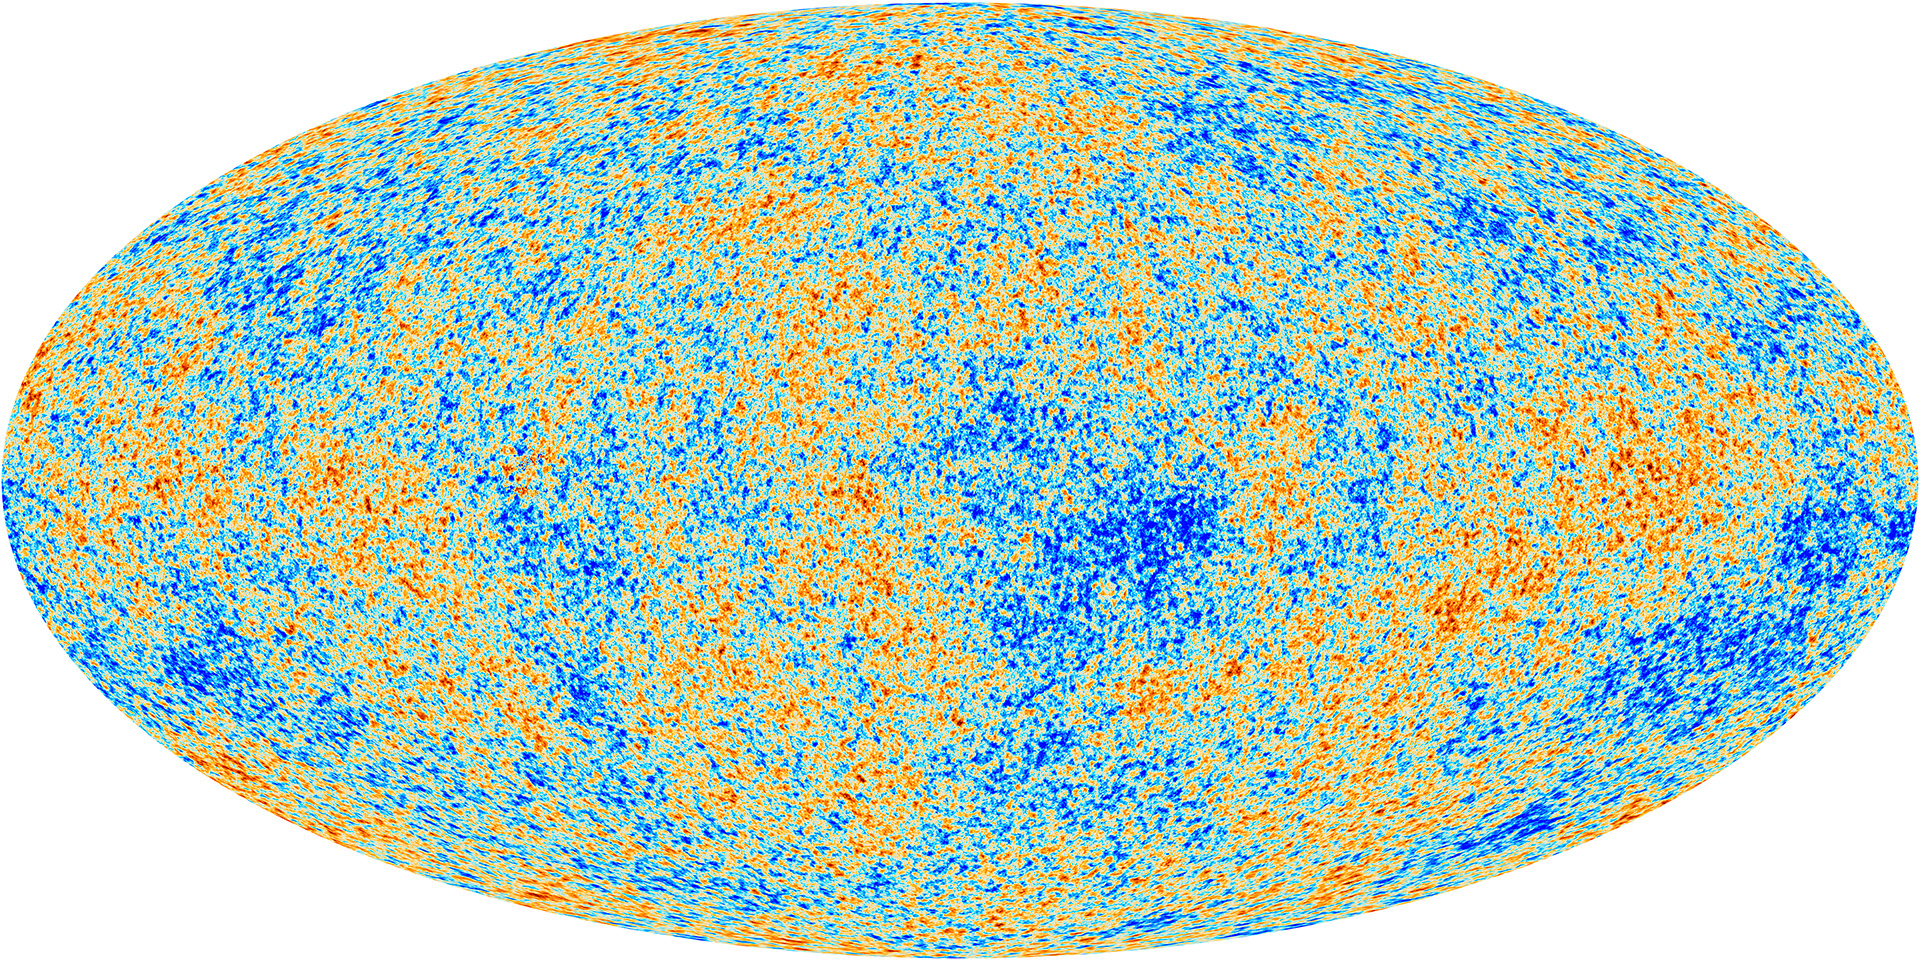
\includegraphics[width=\textwidth]{chapters/outline/figures/planck}
  \caption{Temperature distortions in the cosmic microwave background.}\label{fig:out:planck}
\end{figure}

As cosmologists, nature has been incredibly kind to us. We have been given a near crystal clear snapshot of the universe a mere $380,000$ years after its birth. Maps created by the Planck satellite (Figure~\ref{fig:out:planck}) allow us to determine the patterns of density in the early universe. For cosmologists these density distortions are interesting in two ways. 

First, these perturbations in density are the beginnings of the formation of stars, galaxies and galaxy clusters. If one were to wind the clock forwards from this moment, cosmic structure would be seen coalescing around the regions of higher density.

Second, these distortions tell us a great deal about physics at much earlier times. Observations from particle physics experiments allow us to confidently wind the clock backwards to mere microseconds after the big bang.
However, the expansion of the universe itself allows us to look even further back than this. We now have a wealth of observational evidence that early in its history, the universe underwent a rapid accelerated expansion. This expansion acts as a cosmic magnifying glass, allowing us to observe patterns $\sim10^{-32}$ seconds after the big bang using the universe we see today. The upshot of this is that cosmologists effectively have access to the most powerful particle accelerator imaginable, reaching energies trillions of times greater than the Large Hadron Collider. 

The canonical explanation for the early period of accelerated expansion is the theory of inflation, with quantum fields providing the necessary driving force. This thesis focusses on the initial conditions for inflation; i.e.\ what started this all off.

\section{Kinetic initial conditions}

Traditionally, cosmologists work under the assumption that at these early times the universe was in an effectively eternal inflating state, with no detectable beginning. Chapter~\ref{chap:kd} rigorously proves a result that suggests this picture may be somewhat incomplete. In fact, almost all classical universes begin at a finite time in the past. Moreover, this beginning is dominated by kinetic energy, and not inflating. This provides a novel and arguably simpler mechanism for setting the initial conditions of the universe. More importantly, I also show that this period could have produced a distinct observational signature in the primordial power spectrum of curvature perturbations. Chapter~\ref{chap:kt} details how this mathematical observation fits into more traditional approaches.

As a member of the Planck collaboration, I began to search for evidence of this pre-inflationary phase. Chapter~\ref{chap:rec} details a model-independent reconstruction of the primordial spectrum. Whilst not conclusive, there are tantalising hints of a signal consistent with a pre-inflationary epoch.

\section{Observations in high dimensions}
\begin{figure}[tp]
  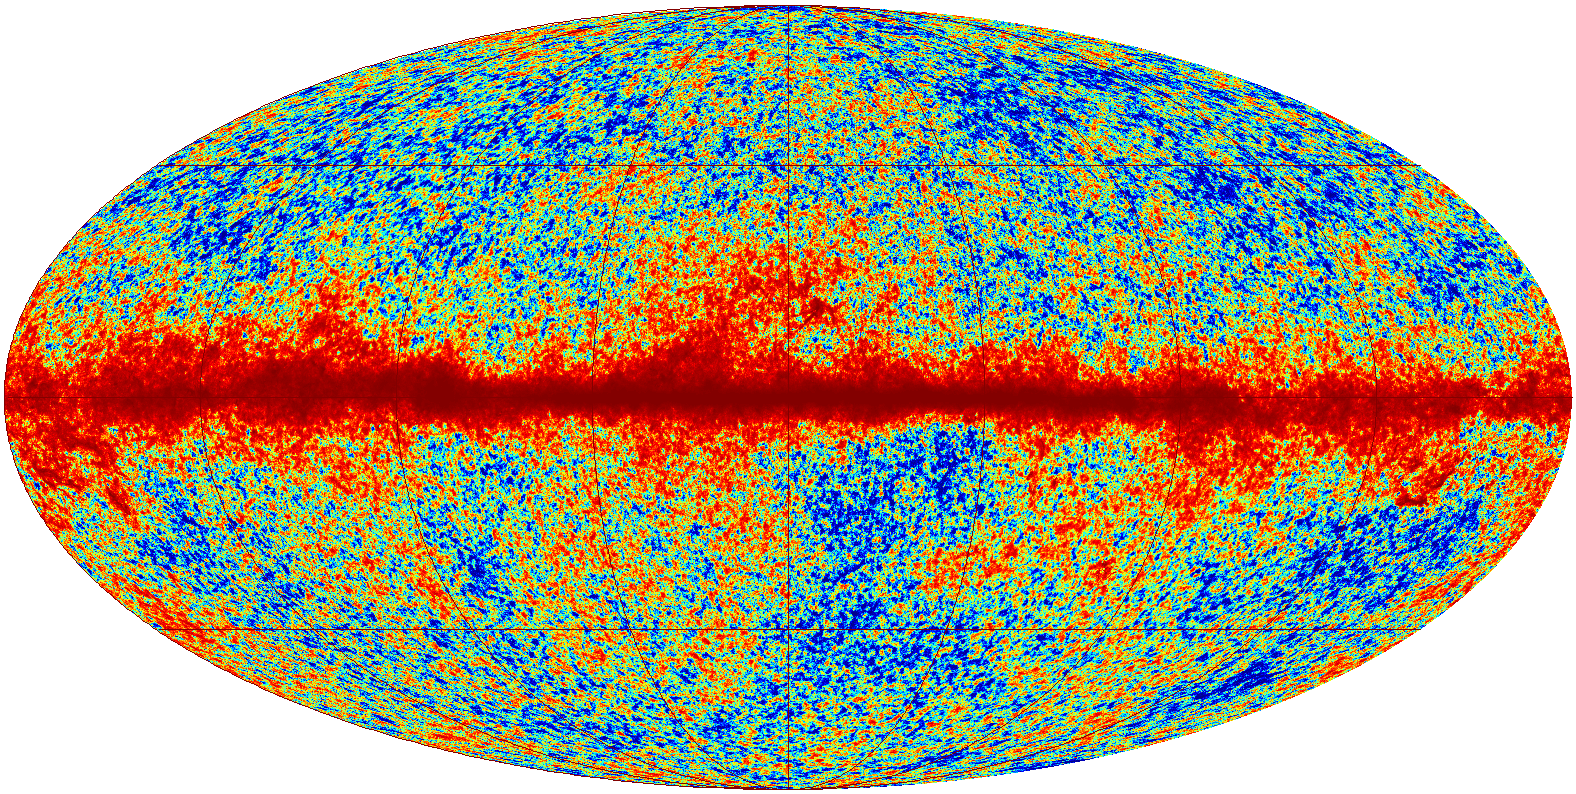
\includegraphics[width=\textwidth]{chapters/outline/figures/planck_galaxy}
  \caption{The microwave sky as seen by Planck}\label{fig:out:planck_galaxy}
\end{figure}
Our microwave sky does not look like Figure~\ref{fig:out:planck}. The sky that Planck actually sees is more akin to Figure~\ref{fig:out:planck_galaxy}. The most notable difference between the two figures is the presence of a red band in the center of the second image, which are the microwaves emitted by our own Milky Way galaxy. In order to observe the signal generated by the beginning of the universe (Figure~\ref{fig:out:planck_galaxy}), we must first take into account the contaminating information of the Milky Way. This requires a sophisticated model of the galaxy, with many parameters that must be simultaneously determined and quantified. 

Whilst attempting to reconstruct the primordial power spectrum (Chapter~\ref{chap:rec}), it became apparent that there was an absence of Bayesian data analysis tools. The techniques available at the time were incapable of navigating and integrating the complicated high-dimensional likelihoods required for my reconstruction.

The Cavendish Astrophysics group has a long history of developing and applying novel Bayesian statistical approaches. With this in mind, I designed and implemented a novel nested sampling algorithm which was christened PolyChord (detailed in Chapter~\ref{chap:pc}). This proved capable of scaling to the dimensionalities required, and reliably computing  the Bayesian evidence, allowing me to produce a model-independent reconstructions of the primordial power spectrum.
As a result, PolyChord was rapidly adopted by many members of the team as their de-facto inference tool

\section{Quantum initial conditions}
My latest work focusses on the quantum mechanical initial conditions of the early universe. A full theoretical treatment of this epoch requires a consideration of quantum fields in curved spacetime. One of the critical issues of this field is that the basic concepts we use to describe quantum particles are not designed to work in the context of gravity as a curved spacetime background. My latest research aims to resolve some of these issues, by building the quantum vacuum around the renormalised stress energy tensor. In essence, I hypothesise that empty space could be better defined as ``lowest energy'' rather than ``particle-less''. I also demonstrated that in the context of the early universe this alternative viewpoint makes detectable predictions which again differ from standard theory. This is detailed in Chapter~\ref{chap:qv}.

Whilst examining this, I realised that I needed a better way of solving the differential equations of the early universe. I succeeded in developing a novel class of extremely efficient numerical methods for solving these, which I term Runge-Kutta-Wentzel-Kramers-Brillioun approaches. RKWKB is explained Chapter~\ref{chap:RK}.

\section{Thesis versus research}
\begin{figure}[tp]
  \centering
  \tikzsetnextfilename{sequence}
  %\tikzset{external/export next=false}

\begin{tikzpicture}[%
    node distance = 5mm,
    writing/.style={%
      text width=30mm,  % default text width
      align=center      % align in center
    },
    component/.style={%
      writing,          % writing style above
    },
    connection/.style={%
      very thick,      % very thick arrows
      >=stealth        % pretty arrow head
    }
]

  \node[component] (KD) at (0,0) {Kinetic dominance\\(Chapter~\protect\ref{chp:kd})};

  \node[below left = of KD, component] (TO)  {Theoretical observations\\(Chapter~\protect\ref{chp:kt})};

  \node[below = of KD, component] (PS) {Power spectrum reconstruction\\(Chapter~\protect\ref{chp:rec})};

  \node[right = of PS, component] (NS) {Nested sampling\\(Chapter~\protect\ref{chp:ens})};

  \node[below = of NS, component] (PC) {\PolyChord{}\\(Chapter~\protect\ref{chp:pc})};

  \node[below = of TO, component] (RE) {Quantum\\ kinetic dominance\\(Chapter~\protect\ref{chp:qv})};

  \node[below = of RE, component] (RK) {RKWKB\\(Chapter~\protect\ref{chp:RK})};

  \node[right = of RK, component] (FUT) {Constraining the kinetically dominated universe\\(Future research)};

    \draw[connection,->] (KD) -- (PS);
    \draw[connection,->] (KD) -- (TO);
    \draw[connection,->] (NS) -- (PC);
    \draw[connection,->] (PC) -- (PS);
    \draw[connection,->] (TO) -- (RE);
    \draw[connection,->] (PS) -- (RE);
    \draw[connection,->] (RE) -- (RK);
    \draw[connection,->] (RE) -- (FUT);
    \draw[connection,->] (PC) -- (FUT);
    \draw[connection,->] (RK) -- (FUT);
    \draw[connection,->] (PS) -- (FUT);

\end{tikzpicture}

  \includegraphics[width=\textwidth]{chapters/outline/plots/sequence.tikz}
  \caption{The ``sequence'' of my research.}\label{fig:out:sequence}
\end{figure}

The theme of this thesis is the interplay between theory, observations and methods. Whilst the thesis divided into two parts, in reality both halves have strongly influenced each other in a manner not necessarily consistent with the sequence of the text. Figure~\ref{fig:out:sequence} shows an approximate set of interactions between the various chapters. Whilst a thesis must be laid out sequentially, actual research is often very non-linear. The degree committee requires that a dissertation be a ``connected account of research'', and whilst this thesis is not sequentially connected, it does at least form a directed acyclic graph.

%
%
%
%
%
%
% Cosmology
% =========
%
\part{Cosmology}
\label{part:cosmology}
%
% Inflationary Cosmology
% ----------------------
%
\chapter{Inflationary Cosmology}
\label{chap:cos}

\section{Introduction}
\label{sec:cos:intro}

I assume a working knowledge of Einstein's theory of general relativity. Review the key concepts mostly to establish notation. Excellent references can be found in~\cite{Wald},~\cite{Hobson} \&~\cite{Dodelson}.

\section{Einstein's gravity}
\label{sec:cos:einsteins_gravity}
\begin{quote}
  {\em Spacetime tells matter how to move;\\ matter tells spacetime how to curve.}\hfill
  --- \johnwheeler{}
\end{quote}

Einstein's theory of general relativity accounts for gravity by removing it as a fundamental force and considering gravitation as a property of spacetime itself. Objects and fields still interact with one another on a spacetime background via the usual forces (electromagnetic, strong and weak nuclear forces). The background spacetime can be thought of as curved, and the perceived effect of gravitation is due to objects moving on straight paths in a curved spacetime. Finally, the curvature (and thus gravitation) is generated by the matter content of the spacetime.

The formalism of Einstein's gravity can be effectively summarised using the Einstein-Hilbert action. An action $S$ is written as a general relativistic integral over a Lagrangian density $\mathcal{L}$:
\begin{equation}
  S = \int\d[4]{x} \sqrt{|g|} \mathcal{L}.
  \label{eqn:cos:generic_lagrangian}
\end{equation}
where the factor of $\sqrt{g}$, $g=\left|\det\left( g_{\mu\nu} \right)\right|$ ensures a relativistic volume element for integration.
We typically decompose the Lagrangian $\mathcal{L}$ into a gravitational and matter part:
\begin{align}
  \mathcal{L} &= \mathcal{L}_G + \mathcal{L}_M,
  \label{eqn:cos:decomp}\\
  \mathcal{L}_G &= \frac{1}{2} \m^2 R,
  \label{eqn:cos:L_grav}
\end{align}
where $R$ is the Ricci scalar and $\mathcal{L}_M$ is the portion of the Lagrangian pertaining to the material content of spacetime. Requiring that the action~\eqref{eqn:cos:generic_lagrangian} is extremal ($\delta S = 0$) yields Einstein's equations:
\begin{equation}
  G_{\mu\nu} = \frac{1}{\m^2}T_{\mu\nu},
  \label{eqn:cos:einsteins_equations}
\end{equation}
where:
\begin{equation}
  T_{\mu\nu} = \frac{-2}{\sqrt{\abs{g}}}\frac{\delta}{\delta g^{\mu\nu}}\left( \sqrt{\abs{g} \mathcal{L}_M} \right),
  \label{eqn:cos:SET_fundamantal}
\end{equation}
is the stress energy tensor, and:
\begin{equation}
  G_{\mu\nu} = R_{\mu\nu} - \frac{1}{2}g_{\mu\nu} R,
  \label{eqn:cos:einstein_tensor}
\end{equation}
is the Einstein tensor. The symmetries of the Einstein tensor~\eqref{eqn:cos:einstein_tensor} mean that there are in fact only six independent equations in~\eqref{eqn:cos:einsteins_equations}. Further, the fact that $\nabla^\mu G_{\mu\nu}=0$ means that the stress energy tensor is conserved:
\begin{equation}
  \nabla_\mu T^{\mu}_{\nu} = 0.
  \label{eqn:cos:SET_conservation}
\end{equation}
This conservation equation can provide a fast means for deriving alternative rearrangements of the Einstein equations.

\section{The smooth, expanding universe}
On the largest scales, we observe the universe to be spatially {\em homogeneous\/} and {\em isotropic}. This justifies the philosophical {\em cosmological principle}, that the universe looks the same whoever and wherever you are. 

In this section, we examine the consequences that these observations have within the context of general relativity, by considering the solutions to the Einstein equations~\ref{eqn:cos:einsteins_equations}.

\subsection{Metric}
\begin{table}
  \centering
  \begin{tabular}{ll}
 \toprule
  Symbol & Definition \\
 \midrule
 \midrule
  $t$ & cosmic time \\
  $X$ & Spatial coordinate \\
  $\chi$ & Comoving radial coordinate \\
  $\theta$ & polar angle \\
  $\phi$ & azimuthal angle \\
  $\Omega$ & solid angle \\
  $a$ & cosmic scale factor \\
  $k=+1$ & closed universe \\
  $k=0$ & flat universe \\
  $k=-1$ & open universe \\
 \bottomrule
\end{tabular}

\caption{Definitions of terms in the FRW metric}\label{tab:cos:metric}
\end{table}

In any general relativistic analysis, it is helpful to restrict the form of the metric via the symmetries of the problem.
Under the assumption of the cosmological principle, the metric may only the Friedmann-Robertson-Walker (FRW) form:
\begin{equation}
  \d{s}^2 = \d{t}^2 - a{(t)}^2 \d{X}^2,
  \label{eqn:cos:FRW_metric}
\end{equation}
where:
\begin{align}
  \d{X}^2 &= \d{\chi}^2 + S_k^2{(\chi)} \d{\Omega}
  \label{eqn:cos:space_element}\\
  \d{\Omega} &= \d{\theta}^2 + \sin^2\theta \d{\phi}^2,
  \label{eqn:cos:angle_element}\\
  S_k^2(\chi) &=
  \left\{
  \begin{array}{rl}
    \sin^2\chi &: k=+1 \\
    \chi^2 &: k=0 \\
    \sinh^2\chi &: k=-1. \\
  \end{array}
  \right.\label{eqn:cos:S_def}
\end{align}
The definitions of these terms can be found in Table~\ref{tab:cos:metric}. 

The form of the metric~\eqref{eqn:cos:FRW_metric} is close to Minkowski. Spatial slices at constant $t$ are spaces with constant curvature, which may be positive, negative or zero (corresponding to a closed, open or flat universe). The time dependency of the spatial part is a scaling by a scale factor $a(t)$. As cosmic time $t$ increases, $a(t)$ evolves, causing the spatial slice to expand or contract (Figure~\ref{fig:cos:comoving_vs_physical}). 



\begin{figure}[tp]
  \centering
  \tikzsetnextfilename{comoving}
  \includegraphics[width=\textwidth]{chapters/inflationary_cosmology/plots/comoving.tikz}
  \caption{The expansion of the universe. As the universe evolves with time, the scale factor $a(t)$ changes. The scale factor $a(t)$ connects {\em comoving coordinates}, $X$ with {\em physical co\"{o}rdinates}, $x=a(t)X$. Comoving variables can be thought of as a time-independent grid, which expands with the universe.\label{fig:cos:comoving_vs_physical}, physical variables are what observers would measure as distances. Hence, in an expanding universe, the physical distance between observers (dots in the diagram above) appears to increase over time, whilst their comoving distance remains the same.}
\end{figure}


\subsection{Dynamics}
In order to obtain the equations governing $a(t)$ and thus the dynamics of the universe, we must make some assumptions about the universes contents. For a smooth universe, one may model its contents as a collection of non-interacting, comoving, uniform, perfect fluids. A perfect fluid in thermodynamic equilibrium has stress-energy tensor:
\begin{equation}
  T^{\mu\nu} = (P+\rho)u^{\mu}u^{\nu} - P g^{\mu\nu} + \Sigma^{\mu\nu},
  \label{eqn:cos:SET_perfect_fluid}
\end{equation}
where $\rho$ is the energy density, $P$ is the pressure, $u^\mu$ is the four velocity of the fluid, and $\Sigma^{\mu\nu}$ is a traceless, symmetric, anisotropic stress term. In accordance with the cosmological principle, we shall assume that in the comoving frame the fluid is stationary $u^\mu = [1,\bzero]$, and uniform $\rho=\rho(t),P=P(t)$, with no anisotropy $\Sigma=0$.  

Applying the metric~\eqref{eqn:cos:FRW_metric} to the Einstein equations~\eqref{eqn:cos:einsteins_equations}, with the stress-energy tensor~\eqref{eqn:cos:SET_perfect_fluid} one finds:
\begin{align}
  \dot{H}+H^2 &= 
  -\frac{1}{6\m^2}\left( \rho + 3P\right), 
  \label{eqn:cos:Raychaudhuri}
  \\
  H^2 &= 
  \frac{1}{3\m^2}\rho - \frac{k}{a^2}, 
  \label{eqn:cos:Friedmann}
\end{align}
%
where $H=\dot{a}/a$ is the Hubble parameter and a dot denotes differentiation with respect to cosmic time, $\dot{f}\equiv df/\d{t}$. These are termed the {\em Raychaudhuri\/} and {\em Friedmann\/} equations respectively, and implicitly govern the dynamics of the scale factor $a(t)$. It should be noted that these equations are not complete, as additionally one requires an equation of state linking $\rho$ and $P$.

\subsection{Basic solutions}
A reasonable model for the universe we observe today is to treat the matter as a multi-component fluid, with each component with its own equation of state:
\begin{equation}
  \rho = \sum_i \rho_i, \qquad P = \sum_i P_i, \qquad P_i = w_i \rho_i,
  \label{eqn:cos:multi_component}
\end{equation}
where $w_i$ is the equation of state parameter. In our universe, we observe matter $(w=0)$, radiation $(w=\frac{1}{3})$ and dark energy $(w=-1)$. We can also notationally model the curvature's scale-factor contribution of $-\frac{k}{a^2}$ as a cosmological fluid with $w=-\frac{1}{3}$. Applying these equations of states, equations~\eqref{eqn:cos:Raychaudhuri} and~\eqref{eqn:cos:Friedmann} may be re-cast as an equation purely in $a$:
\begin{equation}
  {\left( \frac{H}{H_0} \right)}^2 \equiv 
  \frac{1}{H_0^2}{\left( \frac{\dot{a}}{a} \right)}^2 =
  \Omega^\text{(rad)}_0 a^{-4} +
  \Omega^\text{(mat)}_0 a^{-3} + 
  \Omega^\text{(curv)}_0 a^{-2} +
  \Omega^\text{(de)}_0,
  \label{eqn:cos:expansion_history}
\end{equation}
where the present-day $(t=t_0)$ scale factor is chosen to be unity $(a(t_0)=1)$, quantities subscripted with $0$ indicate the present-day  value of the parameter, and the density parameter $\Omega$ is defined as:
\begin{equation}
  \Omega = \frac{\rho}{\rho_\mathrm{c}}, \qquad \rho_\mathrm{c} = {3\m^2H^2},
  \label{eqn:cos:omega_def}
\end{equation}
which measures the fraction of the critical density $\rho_c$ taken up by a given component. Equation~\eqref{eqn:cos:expansion_history} cannot be analytically solved, but if one assumes that one component is dominant, and the rest negligible, then one recovers the solution:
\begin{equation}
  a  \propto
  \left\{
  \begin{array}{ll}
    t^{2/3(w+1)} &: w\ne-1\\
    e^{H_0 t} &: w=-1.\\
  \end{array}
  \right.
\end{equation}
We can see immediately that in a universe dominated by dark energy $(w=-1)$ the expansion is exponential, and in one dominated by radiation $(w=1/3)$, that $a\propto t^{1/2}$, which is a slower expansion than one dominated by matter $a\propto t^{2/3}$. In our universe, where we observe that it is approximately flat, $\Omega_0^{\text{(curv)}}\approx0$, matter now vastly outweighs radiation, and is of the same order of magnitude as dark energy, ${\Omega_0^{\text{(de)}} \approx \Omega_0^{\text{(mat)}} \gg \Omega_0^{\text{(rad)}}}$, we expect an expansion history of the form shown in Figure~\ref{fig:cos:expansion_history}.

\begin{figure}[tp]
  \centering
  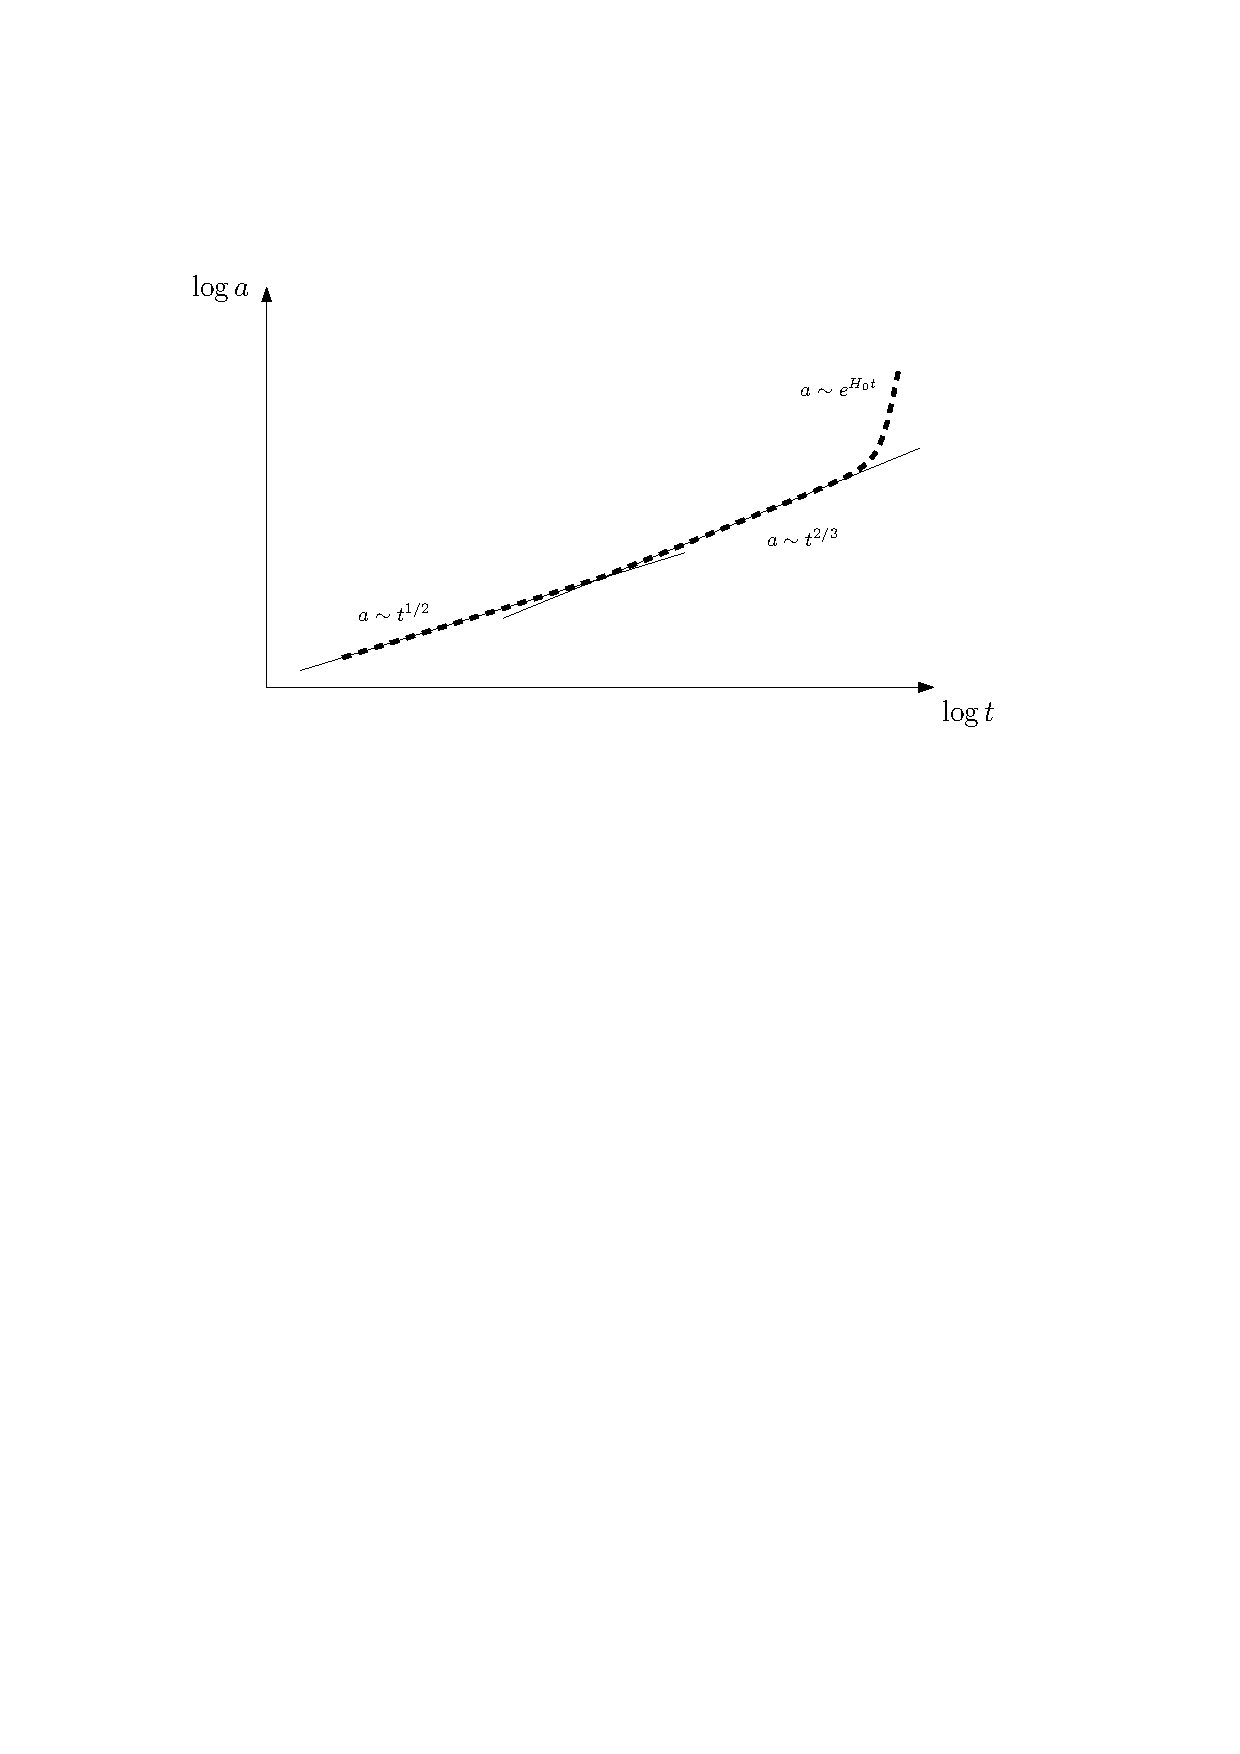
\includegraphics[width=\textwidth]{chapters/inflationary_cosmology/figures/expansion_history}
  \caption{The approximate expansion history of our universe. Initially, the universe is dominated by radiation $a\sim t^{1/2}$. As the universe expands, the photon lose energy as their wavelengths are stretched.  Thus, the universe transitions to a matter dominated $a\sim t^{2/3}$ regime. Finally, the dark energy of the universe overtakes the matter content, and it settles into an exponential expansion $a\sim e^{H_0 t}$\label{fig:cos:expansion_history}}
\end{figure}


\section{Conformal time and redshift}
\subsection{Redshift $z$}
The expansion of the universe causes the wavelengths of photons to increase: Photons have a four-momentum proportional to their wavevector $p^\mu \propto k^\mu$. Since the FRW metric has no explicit $\chi$-dependence for radially travelling photons, $p_\chi$ is conserved: $p_\chi(t_1) = p_\chi(t_2)$. Using the metric to raise the indices, one finds that $p^\chi(t_2)/a(t_2)=p^\chi(t_1)/a(t_1)$. Identifying ${p^\chi \propto k^r \propto \lambda^{-1}}$ where $\lambda$ is the wavelength of the photon, one finds:
\begin{equation}
  \frac{\lambda_2}{\lambda_1} = \frac{a_2}{a_1},
\end{equation}
and thus the wavelengths of photons increase with the expansion of the universe. Physically, the stretching of spacetime stretches the wavelengths of photons.
The redshift $z$ of the photon from some early time $t_1$, relative to the current epoch $t_0$, is defined as usual as:
\begin{equation}
  z = \frac{\lambda_0-\lambda_1}{\lambda_1},
\end{equation}
which gives a relation between the redshift of a photon and the scale factor:
\begin{equation}
  a = \frac{1}{1+z}.
\end{equation}
Since redshift is a physically observable quantity, it provides a cosmology-independent measure of the epoch of the universe (Table~\ref{tab:cos:universe_timeline}).
\begin{table}
  \centering
  \begin{tabular}{ll}
 \toprule
  Epoch & Redshift \\
 \midrule
 \midrule
 Matter-radiation equality &
 $z\sim3400$
 \\
 Recombination &
 $z\sim1089$
 \\
 Dark ages &
 $20<z<1089$
 \\
 First stars &
 $z\sim20$
 \\
 Reionisation &
 $6<z<20$
 \\
 Dark energy-matter equality &
 $z=0.4$
 \\
 Now &
 $z=0$
 \\
 \bottomrule
\end{tabular}

\caption{Recent history of the universe. As redshifts are observable quantities, they should not depend on the specific contents of the universe, and provide a robust measure of cosmic epoch.}\label{tab:cos:universe_timeline}
\end{table}

\subsection{Conformal time $\eta$}

It convenient to define conformal time as:
\begin{equation}
  \eta = \int \frac{\d{t}}{a},
  \label{eqn:cos:conformal_time}
\end{equation}
so that the line element becomes:
\begin{equation}          
  ds^2 = a(\eta)\left( \d{\eta}^2 - d{X}^2 \right).
  \label{eqn:cos:flat_FRW}
\end{equation}
This is often analytically useful, but physically conformal time corresponds to a time coordinate in which photons appear as if they were in flt space: If we consider (without loss of generality) radially travelling photons $\d{\Omega}=0$ the line element is:
\begin{equation}          
  ds^2 = a(\eta)\left( \d{\eta}^2 - \d{\chi}^2 \right).
  \label{eqn:cos:flat_FRW_radial}
\end{equation}
and the metric is conformally equivalent to two-dimensional Minkowski space\footnote{Hence the name ``conformal time''.}. We have thus removed all the complexities of curvature and comoving coordinates. Since photons have a null trajectory, $ds^2=0\Rightarrow \d{\eta} = \pm \d{\chi}$, and therefore  travel in straight lines on spacetime diagrams with $\eta$ and $\chi$ as axes. This considerably simplifies most pictures. It can therefore be thought of as a ``comoving'' time, in analogy with comoving spatial co\"{o}rdinates.\footnote{Alternatively, conformal time is the time measured by a small light clock that expands comovingly with the universe.}

\section{The cosmic microwave background}
\begin{figure}[tp]
  \centering
  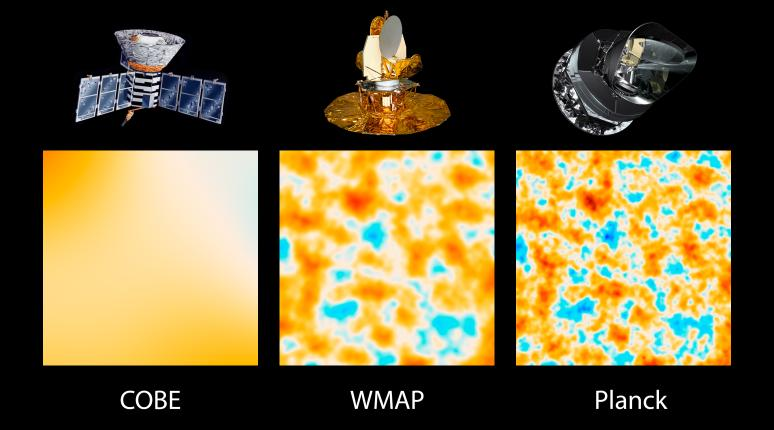
\includegraphics[width=\textwidth]{chapters/inflationary_cosmology/figures/satellites}
  \caption{Microwave satellite pictures.\protect\footnote{Image credit:NASA/JPL-Caltech/ESA}}\label{fig:cos:satellites}
\end{figure}

As we turn telescopes on objects further away from earth, we begin to look appreciably back in time. The radiation from these objects has taken so long to reach us that we can observe the universe in a much younger state than it is now. The furthest galaxies imaged by the Hubble space telescope are more than 13 billion years old. Many of these objects are so far away that they have redshifted out of the visible spectrum and into the infra-red. If we look beyond, we enter the dark ages of the universe, before the first stars had turned on. This would appear to be the end of the observational story.

However, from behind the dark ages, there is a background of microwaves. These would originally have been emitted as X-rays, but have redshifted all the way down to the microwave end of the spectrum.\footnote{Incidentally, this means that at around redshift $3<z<7$, the universe would have been bathed in optical light. However, it would have been at too low an intensity to be visible to the naked eye. Assuming a threshold of the human eye of $10^{-6}\mathrm{cd}\;\mathrm{m}^{-2}$, the CMB would stop being visible at $z\sim200$, at which point it would have been white.}. This uniform backdrop of radiation is our direct image of the universe as it was at redshift $z\sim1000$, when the universe was a mere $300,000$ years old.

Since its first (accidental) detection in 1964 by~\cite{PenziasWilson}, a succession of hundreds of microwave telescopes, both on the ground and in space, have sharpened our image of this (Figure~\ref{fig:cos:satellites}).
The cosmic microwave background (CMB) is found to be:
\begin{enumerate}
  \item Isotropic to one part in $10^{5}$.
  \item A near-perfect blackbody spectrum, with $T_0=2.7254(5)$.
  \item Anisotropic with non-trivial power spectrum.
\end{enumerate}

\section{Problems in the CMB}
\subsection{Flatness problem}
The degree to which the universe is not flat can be measured by re-writing the Friedmann equation~\eqref{eqn:cos:Friedmann} in terms of $\Omega$ as in~\eqref{eqn:cos:omega_def}:
\begin{equation}
  1-\Omega = -\frac{k}{{(aH)}^2} \equiv \Omega_k.
  \label{eqn:cos:friedmann_omega}
\end{equation}
In terms of these kind of variables, the Raychaudhuri equation~\eqref{eqn:cos:Raychaudhuri} is:
\begin{equation}
  \frac{\d{\log aH}}{\d{\log a} } = -\frac{1}{2}\Omega(1+3w),
  \label{eqn:cos:raychaudhuri_omega}
\end{equation}
where here $w=P/\rho$ is not necessarily constant.
Taking absolute logarithms of~\eqref{eqn:cos:friedmann_omega}, differentiating and applying~\eqref{eqn:cos:raychaudhuri_omega} yields:
\begin{equation}
  \frac{\d{\log |\Omega-1|}}{\d{\log a} } = \Omega(1+3w).
  \label{eqn:cos:instability}
\end{equation}
One can see from this that a flat universe $(\Omega=1)$ is an unstable point of equilibrium of these equations, providing that $1+3w>0$. For both matter (${w=0}$) and radiation (${w=\frac{1}{3}}$), the universe is rapidly driven away from flatness as the universe expands. This is natural, as the effect of traditional mass-energy is to increase the curvature of space with time

This presents a problem. The universe we see today is measured to be flat to at least one part in $10^{-2}$, which means that at earlier times it would have been even flatter still. Given that within the context of cosmology there is no a-priori reason to believe the universe should be exactly flat, this requires a unreasonable quantity of fine tuning. It would be more satisfactory if we had a dynamical reason to explain why the universe is as flat as it is.

As well as revealing the problem, equation~\eqref{eqn:cos:instability} also provides a solution. If for some period $w<-1/3$ at some earlier time, then~\eqref{eqn:cos:instability} says that $\Omega=1$ is an attractor state. The Raychaudhuri equation shows that:
\begin{equation}
  \ddot{a} \propto -(1+3w).
  \label{eqn:cos:Raychaudhuri_acc}
\end{equation}
Thus, the condition that $w<-1/3$ is equivalent to requiring that at some point early in its history the universe was {\em accelerating\/} $\ddot{a}>0$. It is also equivalent to having a form of matter which satisfies:
\begin{equation}
  P < -\frac{1}{3}\rho,
  \label{eqn:cos:SEC_violation}
\end{equation}
which can be recognised as a violation of the {\em strong energy condition}.

\subsection{Horizon problem}
\begin{figure}[tp]
  \centering
  \tikzsetnextfilename{horizon_problem}
  \includegraphics[width=\textwidth]{chapters/inflationary_cosmology/plots/horizon_problem.tikz}
  \caption{The horizon problem. From our position, we observe the CMB as a surface at some earlier time. The homogeneity of the CMB suggests that there must have been some physical mechanism to smooth it out. However, in cosmologies with traditional matter, there is not enough time before the CMB to allow this to occur. In fact, the CMB appears to be made up of causally disconnected regions. There is thus no dynamical reason as to why these disconnected regions should show such similar physical conditions. As a rough guideline, a causal patch is roughly a thumb-width on the sky.}\label{fig:cos:horizon_problem}
\end{figure}
The near-perfect isotropy of the CMB also presents a problem. Our image of the CMB represents the universe as it was some 300,000 years after it was born. In cosmologies with traditional forms of matter, there is quantitatively not enough time before the CMB for {\em any\/} dynamical process to allow the universe to reach a homogeneous state. Indeed, the CMB can be seen to be made up of some $10^{5}$ causally disconnected patches, with the causal patch size approximately one thumbs-width on the sky. This can be seen graphically in Figure~\ref{fig:cos:horizon_problem}.

Note that we may resolve this problem with an accelerated phase as well (Figure~\ref{fig:cos:horizon_problem_resolved}). An accelerated phase pushes any singularity far back into the conformal past. This means that there is more than enough time for the universe to dynamically come to equilibrium. In fact, a detailed analysis shows that this accelerated epoch acts as a ``smoothing'' effect on a given causal patch, yielding a homogeneous universe from any generic initial conditions.


\begin{figure}[tp]
  \centering
  \tikzsetnextfilename{horizon_problem_resolved}
  \includegraphics[width=\textwidth]{chapters/inflationary_cosmology/plots/horizon_problem_resolved.tikz}
  \caption{Horizon problem resolved. An early accelerating phase pushes the singularity far into the conformal past, meaning there is more than enough time for the CMB to come to equilibrium.\label{fig:cos:horizon_problem_resolved}}
\end{figure}

\subsection{An accelerating universe}
One may think of both of the above problems in terms of a problem with the ``Cauchy initial conditions'': on some early spatial slice of the universe, the values of cosmological parameters $X$ and $\dot{X}$ was extremely uniform. These correspond to the horizon and flatness problems respectively. An early accelerated phase in the universe history acts to ``stretch out'' a small patch of some generic early universe to cosmic scales. We should therefore expect universes with accelerated early epochs to have generically smooth cosmic microwave backgrounds.

\section{Inflation}
The canonical way to explain this early accelerated phase is via the phenomenon of {\em inflation}. This early accelerated phase will have occurred when the universe was at extremely high energy, which suggests that we should turn to particle physics phenomenology.
It turns out if we consider even the most simple particle physics models in the context of general relativity, these are capable of generating a sustained accelerated phase.

\subsection{Basic theory}
Consider the Lagrangian:
\begin{equation}
  \mathcal{L}_\phi = \frac{1}{2}\nabla^\mu\phi\nabla_\mu\phi - V(\phi).
  \label{eqn:cos:scalar_field_lagrangian}
\end{equation}
This represents a scalar field $\phi$, minimally coupled to gravity with some unspecified potential $V$.  Inserting this into~\eqref{eqn:cos:SET_fundamantal} yields a stress energy tensor of:
\begin{equation}
  T^{\mu}_{\nu} = \nabla^\mu\phi\nabla_\nu\phi - \left( \frac{1}{2}\nabla^\alpha\phi \nabla_\alpha\phi - V(\phi)  \right)\delta^{\mu}_{\nu}.
  \label{eqn:cos:scalar_field_SET}
\end{equation}
If we initially assume in accordance with the cosmological principle that the field has no spatial dependence $\phi = \phi(t)$, then the stress energy tensor becomes:
\begin{align}
  T^{0}_{0} &=\frac{1}{2}\dot\phi^2 + V(\phi) = \rho,
  \label{eqn:cos:scalar_field_rho}\\
  T^{i}_{j} &=-\left[ \frac{1}{2}\dot\phi^2 - V(\phi)\right]\delta^{i}_{j} = -P\delta^{i}_{j}.
  \label{eqn:cos:scalar_field_P}
\end{align}
Thus, a homogeneous scalar field acts as a perfect fluid with pressure and density as shown above. In order to derive the non-trivial and time dependent equation of state, we need to generate an equation of motion for $\phi$. This can be done other by extremising $S_\phi = \int \d[4]{x} \sqrt{|g|} \mathcal{L}_\phi$, or by applying the continuity equation~\eqref{eqn:cos:SET_conservation} to the stress energy tensor~\eqref{eqn:cos:scalar_field_SET}: 
\begin{equation}
  0 = \ddot{\phi} + 3 H \dot{\phi} + \frac{d}{d\phi}V(\phi).
  \label{eqn:cos:KG}
\end{equation}
The middle term involving $H$ is the term that arises as a result of including the effects of gravity (i.e.\ an expanding universe). The homogeneous value of the scalar field $\phi$ satisfies the equation of a harmonic oscillator in potential $V(\phi)$ with a frictional term $H$.
To get an equation for $H$, we use the Raychaudhuri equation~\eqref{eqn:cos:Raychaudhuri} along with our formulae~\eqref{eqn:cos:scalar_field_rho}~\&~\eqref{eqn:cos:scalar_field_P} for $\rho$ and $P$, to find:
\begin{equation}
  \dot{H}+H^2 = -\frac{1}{3\m^2}\left(\dot{\phi}^2-V(\phi)\right).
  \label{eqn:cos:ray_scalar}
\end{equation}
Equation~\eqref{eqn:cos:KG} represents space telling matter how to move and equation~\eqref{eqn:cos:ray_scalar} represents matter telling space how to curve. These equations are tightly coupled, and result in far less trivial behaviour compared with a simple perfect fluid.


\subsection{Phenomenology}
One way to trigger an accelerated phase is to set the inflaton as trapped in a false vacuum (Figure~\ref{fig:cos:potential}). This sets $\dot{\phi}=0$, $V(\phi)=V_0$ and therefore $H=H_0=V_0/3\m^2$ and $a\sim e^{H_0t}$, which is an exponential and therefore accelerated expansion. However, to end this accelerated phase, the inflaton would have to tunnel quantum mechanically out of its false vacuum. It turns out that the false vacuum is too stable, and results in unphysical predictions.

\begin{figure}[tp]
  \centering
  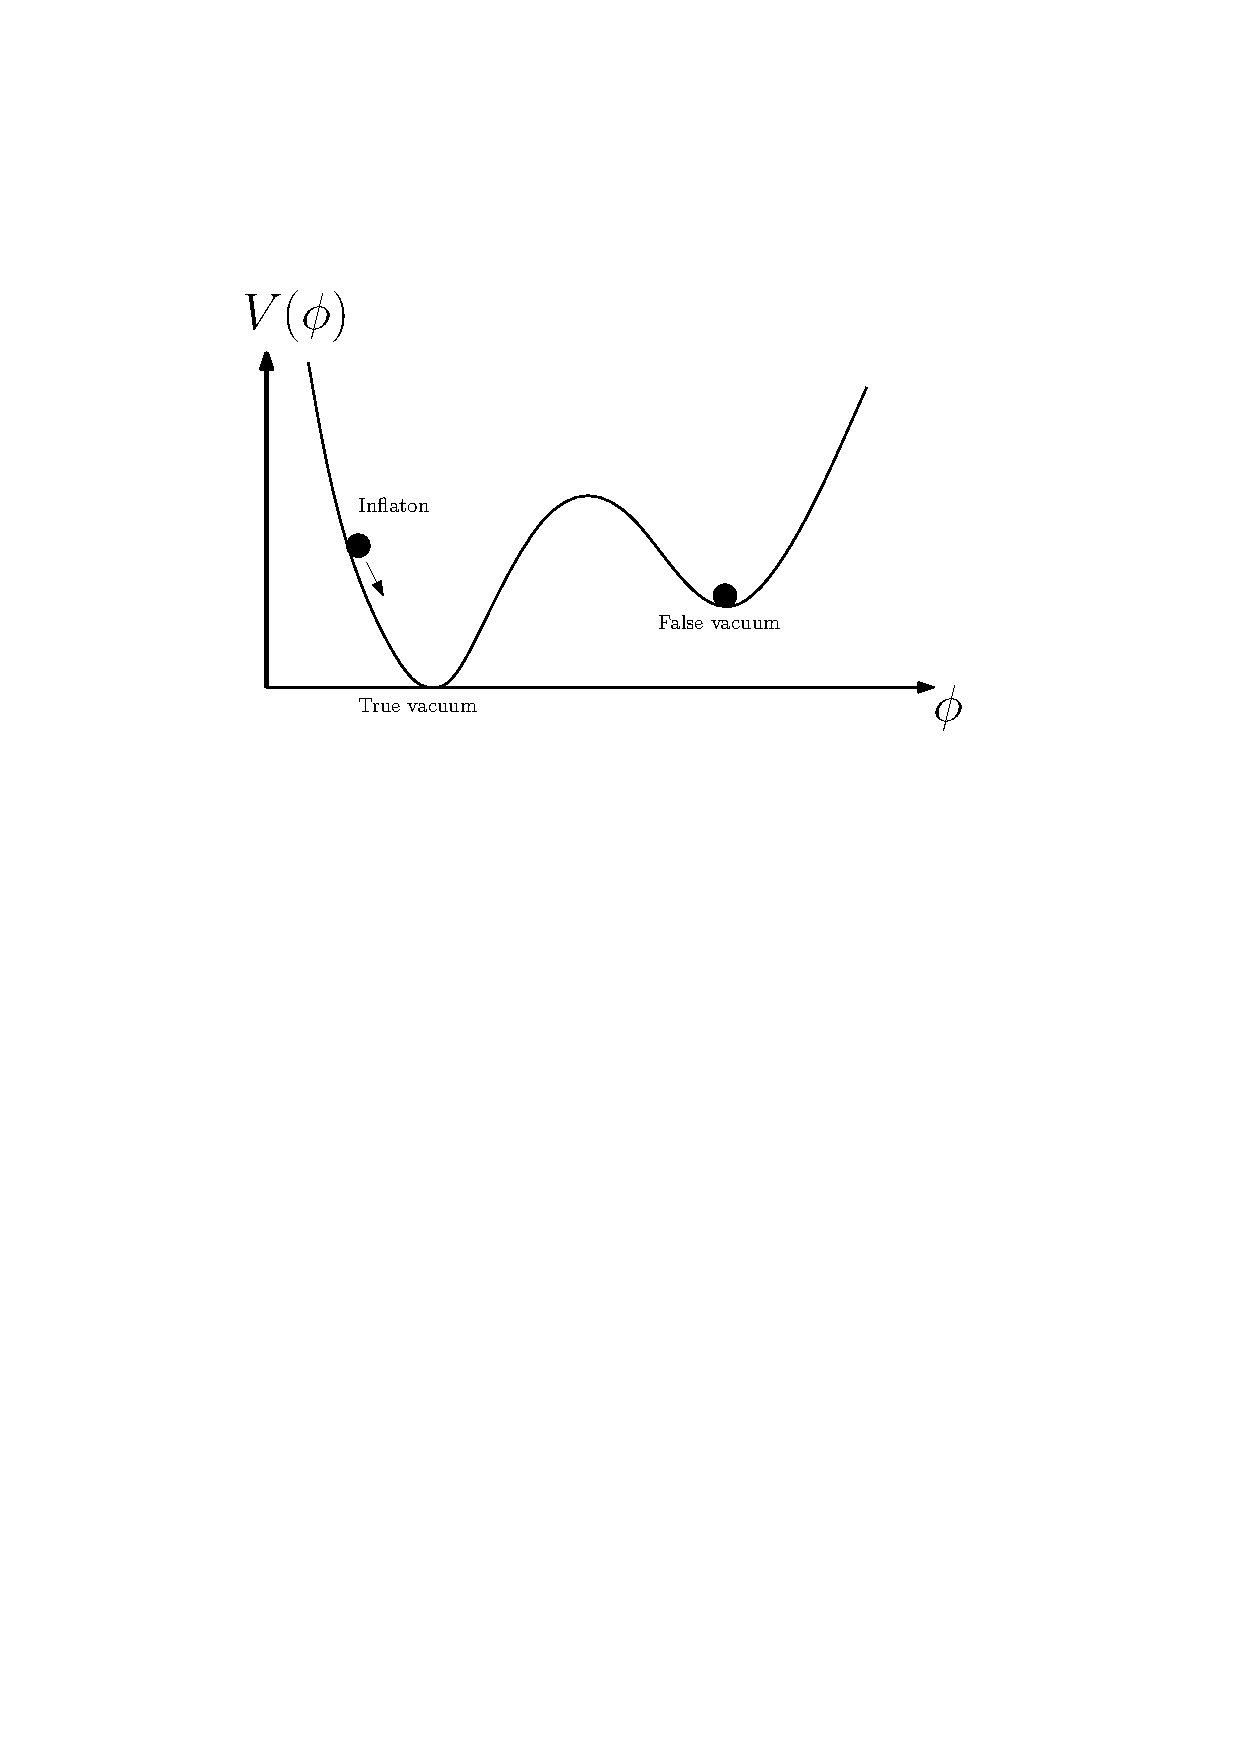
\includegraphics[width=\textwidth]{chapters/inflationary_cosmology/figures/potential}
  \caption{An example inflationary potential.}\label{fig:cos:potential}
\end{figure}

In fact, one does not need a false vacuum, one merely needs the inflaton to be rolling slowly down the potential with its speed small in comparison to the potential energy:
\begin{equation}
  \dot{\phi}^2 \ll V(\phi).
  \label{eqn:cos:slow_roll}
\end{equation}
In this case, one still has the Hubble parameter $H\approx H_0$ being approximately constant and therefore exponential expansion. Since the frictional term in~\eqref{eqn:cos:KG} robs the particle of energy, one finds that in fact these slowly rolling phases are generic attractors for most inflationary potentials. All one requires is that the inflaton begins a reasonable way from the potential minimum.

Thus, a very general scalar particle is capable of triggering a generic exponential accelerated expansion. This epoch of the universe is termed inflation, and the particle of the field $\phi$ the inflaton.

\subsection{Reheating}
Inflation finishes when the inflaton reaches its true vacuum, and oscillates about its minimum. One then imagines that the inflaton then decays into more traditional matter in a period called reheating. This is theoretically interesting and an area of active research. As we shall see however, for the purposes of setting initial conditions on the remainder of the contents of the universe, reheating can often be ignored.




\section{The perturbed universe}
Observationally, the real universe is not perfectly smooth.\footnote{For example, the fact that you are reading this thesis indicates that there must be some departure from homogeneity}
We may treat the smooth FRW metric as a 0\textsuperscript{th} order approximation, to the universe, and expand about this solution using perturbation theory. In general then, we write each quantity as:
\begin{equation}
  X(t,\vx) = X(t) + \delta X(t,\vx).
  \label{eqn:cos:expansion}
\end{equation}
Since in the early universe the perturbations were small $\delta X \ll X$, we may expand all equations to linear order with very high accuracy.

\begin{table}
  \centering
  
\begin{tabular}{lll}
 \toprule
  Symbol & Definition \\
 \midrule
 \midrule
 \(\Phi\) & lapse \\
 \(B_i\) & shift \\
 \(\Psi\) & (spatial) curvature perturbation  \\
 \(E_{ij}\) & (spatial) shear (3-tensor) \\
 \bottomrule
\end{tabular}

  \caption{Definitions of terms in the perturbed FRW metric}\label{tab:cos:perturbed_metric}
\end{table}


\subsection{Metric perturbation}
A general perturbation of the FRW metric will take the form:
\begin{equation}
  ds^2 = (1+2\Phi)\d{t}^2 -2a B_i \d{x}^i \d{t}  -a^2 \left[ \left( 1 - 2 \Psi \right)\delta_{ij} + 2E_{ij} \right] \d{x}^i \d{x}^j,
  \label{eqn:cos:FRW_perturb}
\end{equation}
where the various terms in the above expression are defined in Table~\ref{tab:cos:perturbed_metric}, and ${\Phi,B_i,\Psi,E_{ij}\ll1}$ are small. 

\subsection{Matter perturbation}
Perturbations of the matter content will take the form:
\begin{equation}
  \rho = \rho + \delta \rho, \qquad 
  P = P + \delta P, \qquad
  u^\mu = \left[ 1-\Phi, a^{-2} \delta q^i/(\rho+P)\right].
  \label{eqn:cos:matter_perturb}
\end{equation}
The density and pressure perturbations are self-explanatory. The perturbation to the fluid velocity is first chosen so that $u^\mu u_\mu=1$ to first order, and $\delta q^i$ is the perturbation to the momentum density. The advantage of this is that for non-interacting fluids, $\delta\rho$, $\delta P$ and $\delta q^i$ are all additive, as in equation~\eqref{eqn:cos:multi_component}. We have neglected a perturbation to the anisotropic stress. Anisotropic stress may be included if desired, but is typically not a physical phenomenon. 

At some point one must also assume an equation of state for the fluid which provides equations to constrain $P$ and $\rho$. One can remain fairly general by splitting the pressure perturbation into adiabatic and entropic parts:
\begin{equation}
  \delta P = \delta P_\mathrm{ad} + \delta P_\mathrm{en},
  \label{eqn:cos:adiabatic_entropic}
\end{equation} 
where:
\begin{equation}
  \frac{\delta P_\mathrm{ad}}{\dot{P}} = \frac{\delta\rho}{\dot{\rho}}.
  \label{eqn:cos:adiabatic}
\end{equation} 
In most cases, we limit ourselves to adiabatic matter $\delta P_\mathrm{en}=0$.
This is not particularly restrictive, and is naturally satisfied by the equations of state~\eqref{eqn:cos:multi_component}.

The scalar field perturbation is similarly simple:
\begin{equation}
  \phi = \phi + \delta\phi.
\end{equation}

\subsection{Fourier modes and scalar-vector-tensor decomposition}
In general, the Einstein equations~\eqref{eqn:cos:einstein_tensor} are non-linear, second order, partial differential equations and are therefore extremely challenging to solve. Perturbing about a background as in the previous section yields linearised versions of the Einstein~\eqref{eqn:cos:einsteins_equations} and conservation equations~\eqref{eqn:cos:SET_conservation}:
\begin{align}
  \delta G_{\mu\nu} &= \frac{1}{\m^2}\delta T_{\mu\nu},
  \label{eqn:cos:einsteins_equations_perturb} \\
  \nabla_\mu\delta T^{\mu}_{\nu} &=0,
  \label{eqn:cos:SET_conservation_perturb}
\end{align}
which greatly simplifies the analysis.  
We may go further and exploit the symmetries of the background unperturbed universe to make life even easier.

First, a general field $\varphi(t,\vx)$ can be written in Fourier modes as:
\begin{align}
  \varphi(t,\vk) &= \int \d[3]{\vx}\: \varphi(t,\vx) e^{-i\vk \cdot \vx},\\
  \varphi(t,\vx) &= \int \frac{\d[3]{\vk}}{{(2\pi)}^3}\: \varphi(t,\vx) e^{i\vk \cdot \vx}.
\end{align}
The translational invariance of the unperturbed universe means that the Fourier modes of the perturbations decouple, turning spatial derivatives into multiples of wavevectors. 
It is worth remarking that the above decomposition is specifically for a flat universe. There are analogous approaches for the open and closed cases, but for simplicity we shall keep to the flat case. 

Second, a general spatial vector field $v_i$ and a symmetric tensor field $T_{ij}$ can be decomposed into helicity modes as:
\begin{align}
  v_i =& \partial_i v + v_i,   \nonumber\\
  &(\partial^k v_k=0), \\
  T_{ij} =& (\partial_i\partial_j - \frac{\delta_{ij}}{3}\partial^k\partial_k)T + \frac{1}{2}(\partial_i T_j + \partial_j T_i) + T_{ij} \nonumber,\\ 
  &(\partial^k T_{ki} = \partial^k T_k = 0),
\end{align}
so $v$ and $T$ are helicity scalars, $v_i$ and $T_i$ are divergenceless 3-vectors and $T_{ij}$ is a divergenceless, symmetric, traceless 3-tensor\footnote{Note the overloading: $v$ and $T$ have different meanings on either side of each equation.}.
  The rotational invariance of the unperturbed universe means that the spatial vector and 3-tensor perturbations also decouple.

We may therefore decompose the all perturbations into Fourier components and scalar, vector and tensor parts, decoupling the modes into three parallel analyses without spatial derivatives.

For simplicity, we shall focus on the scalar part of the analysis, since vectors generically decay under an accelerated expansion, and tensors have extremely simple dynamics.

\subsection{Gauge choice}
Observant readers will have noted that there are too many perturbation variables and not enough constraints.
This lack of constraint arises from the fact that the split into background and perturbation $X=X+\delta X$ implied by~\eqref{eqn:cos:expansion} is more subtle than first appears. 

In addition to perturbing the dynamical variables, one can also perturb the coordinate system:
\begin{align}
  t &\rightarrow t + \delta t,
  \label{eqn:cos:gauge_t}
  \\
  x^i &\rightarrow x^i  + \delta x^i,
  \label{eqn:cos:gauge_x}
\end{align}
where in general the small perturbations $\delta t$ and $\delta x^i$ are functions of time and space.
For a generic scalar field $\varphi = \varphi(t,x^i)$, this coordinate perturbation will cause an alteration of the field value:
\begin{equation}
  \varphi \rightarrow \varphi - \dot{\varphi}\delta t - \partial_i\varphi\delta x^i.
\end{equation}
This means that it is easy to conflate ``true'' perturbations in the variables with coordinate perturbations. In the extreme limit of no dynamical perturbation, one can see that the co\"{o}rdinate transformation~\eqref{eqn:cos:gauge_t}~\&~\eqref{eqn:cos:gauge_t} will in in generate a ``false'' perturbation in $\varphi$ of $\delta\varphi = -\dot{\varphi}\delta t - \partial_i\varphi\delta x^i$.

Careful calculation will show that in fact the transformation of the dynamical scalar variables under~\eqref{eqn:cos:gauge_t}~\&~\eqref{eqn:cos:gauge_x} is in fact:\footnote{NB\@: we have decomposed the spatial perturbation as $\delta x^i = \partial^i \delta x + \delta x^i$.}
\begin{align}
  \Phi &\rightarrow \Phi - \delta \dot{t}, &
  \Psi &\rightarrow \Psi +H \delta t,  \nonumber\\
  B &\rightarrow B + \delta t/a - a\delta \dot{x}, &
  E &\rightarrow E - \delta x, \nonumber\\
  \delta\rho &\rightarrow \delta\rho - \dot{\rho}\delta t, &
  \delta P &\rightarrow \delta P - \dot{P}\delta t, \nonumber\\
  \delta q &\rightarrow \delta q + (\rho+P)\delta t,&
  \delta \phi &\rightarrow \delta \phi - \dot{\phi}\delta t.
\end{align}
By choosing an appropriate coordinate transformation, one can remove the additional dynamical variables that are unconstrained by the Einstein equations. This is typically done by setting some of the perturbation variables equal to zero. This procedure is termed a {\em gauge choice}.\footnote{$\delta X$ is defined as the difference between the value $X$ has in the physical (perturbed) spacetime, and the value $X$ has in the background (unperturbed) spacetime. This can only be done if there is a prescription for identifying points between the two spacetimes, and in the language of differential geometry, this is termed a {\em gauge choice}.}
Examples of popular gauge choices can be found in Table~\ref{tab:cos:gauge_choice}.

Whilst choosing a gauge will give one a set of soluble equations, the question still remains whether the perturbations really are ``true'', or in some-way coordinate-dependent. A more robust approach is to avoid the issue entirely and define the gauge independent variables:
\begin{align}
  \Phi^{(B)} &=  \Phi - \dot{T}, &
  \Psi^{(B)} &=  \Psi + HT, \nonumber \\
  \delta\rho^{(B)} &= \delta\rho - \dot{\rho}T, &
  \delta P^{(B)} &= \delta P - \dot{P}T, & \nonumber\\
  \delta q^{(B)} &= \delta q - (\rho + P)T, &
  \delta \phi^{(B)} &= \delta \phi - \dot{\phi}T, 
\end{align}
where $T = a^2[\dot{E}-B/a]$. These variables remain unchanged under gauge transformations, and are independent of coordinate perturbations. Any perturbation in these variables cannot be ``gauged away''. Of course, these are not unique as any linear combination of them is also gauge-invariant, but the above set results in a reasonable basis. 

Procedurally, one of  the most powerful approaches is to choose the Newtonian gauge ${B=E=B_i=0}$. In this gauge, $X^{(B)}=X^{(\text{Newt.})}$. At the end of the computation, we may note that any equations in $X^{(\text{Newt.})}$ will be manifestly gauge-invariant, so we may re-promote all variables $X^{(\text{Newt.})}$ to the gauge-invariant ones $X^{(B)}$.


\begin{table}
  \centering
  \begin{tabular}{ll}
 \toprule
  Name & Definition \\
 \midrule
 \midrule
 Synchronous & \(\Phi=B=0\) \\
 Newtonian & \(B=E=0\) \\
 Uniform density & \(\delta\rho=0\) and e.g.\ \(E=0\) \\
 Comoving & \(\delta q = E = 0\) \\
 Comoving orthogonal & \(\delta q = B = 0\) \\
 Spatially-flat & \(\Psi=E=0\) \\
 \bottomrule
\end{tabular}

\caption{Popular gauge choices for the scalar components of the metric}\label{tab:cos:gauge_choice}
\end{table}

\section{Comoving curvature perturbation}

\subsection{Classical behaviour}
It is convenient to examine the gauge-invariant variable:
\begin{equation}
  \mathcal{R} = \Psi - \frac{H}{\rho+P}\delta q.
  \label{eqn:cos:CCP}
\end{equation}
This is termed the {\em comoving curvature perturbation}, since in the comoving gauge ($\delta q=0$) $\mathcal{R}=\Psi$.
After some effort, the Einstein equations~\eqref{eqn:cos:einsteins_equations}~\&~\eqref{eqn:cos:einsteins_equations_perturb} and conservation equations~\eqref{eqn:cos:SET_conservation}~\&~\eqref{eqn:cos:SET_conservation_perturb} evaluated using the perturbed metric~\eqref{eqn:cos:FRW_perturb} and the perturbed stress energy tensor~\eqref{eqn:cos:SET_perfect_fluid}~\&~\eqref{eqn:cos:matter_perturb} yield:
\begin{equation}
  \frac{d \mathcal{R}}{d \log a} = 
  -\frac{k^2}{a^2}\frac{\dot{P}}{\dot{\rho}}\frac{\mathcal{R}}{(5\rho + 3P)}
  -\frac{\delta P_\mathrm{en}}{\rho+P}.
\end{equation}
For adiabatic perturbations $\delta P_\mathrm{en}=0$, and given that $\rho,P\sim H^2$, the above equation says that: $\frac{d\log \mathcal{R}}{d\log a} \sim \frac{k^2}{a^2H^2}$. As the universe inflates, $k\ll aH$, and $\mathcal{R}$ ``freezes out'' and becomes constant.

\subsection{Quantum behaviour}
Using the Lagrangians are defined by equations~\eqref{eqn:cos:L_grav}~\&~\eqref{eqn:cos:scalar_field_lagrangian}, we may define the action:
\begin{equation}
  S = \int \d[4]{x}\sqrt{|g|}\mathcal{L}_G + \mathcal{L}_\phi.
\end{equation}
If we expand this action to second order in $\mathcal{R}$, we find (after some effort):
\begin{equation}
  S^{(2)} = \int \d[4]{x}\: a^3 \frac{\dot{\phi}^2}{H^2}\left[ \mathcal{\dot{R}}^2 -a^{-2}{\left( \delta_i\mathcal{R} \right)}^2 \right].
\end{equation}
Switching to conformal time and defining:
\begin{equation}
  v = z \mathcal{R}, \qquad
  z = \frac{a \dot{\phi}}{H},
\end{equation}
the action becomes:
\begin{equation}
  S^{(2)} = \int \d[4]{x}\: \left[ {\left( v^{\prime} \right)}^2 - {\left( \partial_i v \right)}^2 + \frac{z^{\prime\prime}}{z}v^2\right],
\end{equation}
where primes denote derivatives with respect to conformal time.

To quantise, we promote the field variable $v$ to a quantum operator, and write it as a Fourier superposition:
\begin{equation}
  v = \int \frac{\d[3]{\vk}}{{\left( 2\pi \right)}^3}
  \left[ 
    \chi_k^{\phantom\ast}(\eta) a_\vk^{\phantom\dagger}e^{i\vk\cdot\vx} + 
    \chi_k^\ast(\eta) a_\vk^{\dagger}e^{-i\vk\cdot\vx}  
  \right],
  \label{eqn:cos:mode_func_sum}
\end{equation}
of mode functions $v_\vk = \chi_k a_\vk$.
Requiring that the canonical commutator relation:
\begin{equation}
  [ a_{\vk^{\phantom\prime}}^{\phantom\dagger}, a_{\vk^{\prime}}^{\dagger}] = {\left( 2\pi \right)}^3\delta^{(3)}\left( \vk^{\phantom\prime}-\vk^{\prime} \right),
  \label{eqn:cos:commutator}
\end{equation}
holds true, then the wavefunction $\chi_k(\eta)$ must satisfy:
\begin{align}
  \chi_k^{\prime\prime} + \left( k^2 - \frac{z^{\prime\prime}}{z} \right) \chi_k &=0,
  \label{eqn:cos:mode_func}
  \\
  {\chi_k^{\phantom\ast}}^{\prime} 
  {\chi_k^{\ast}}^{\phantom\prime} 
  -
  {\chi_k^{\ast}}^{\prime} 
  {\chi_k^{\phantom\ast}}^{\phantom\prime} 
  &= -i.
  \label{eqn:cos:mode_func_normalisation}
\end{align}
\subsection{de-Sitter limit}
A perfectly inflating universe is a de-Sitter space with:
\begin{equation}
  H=\text{const}\Rightarrow \quad a = \frac{1}{H(\eta_\mathrm{end}-\eta)} \propto e^{Ht}, \quad -\infty<\eta<\eta_\mathrm{end}.
  \label{eqn:cos:de-sitter}
\end{equation}
Thus, in a pure de-Sitter space, ${z^{\prime\prime}/z = a^{\prime\prime}/a= 2{(\eta_\mathrm{end}-\eta)}^{-2}}$ and the differential equation~\eqref{eqn:cos:mode_func} has the general solution:
\begin{align}
  \chi_k = &A_k \frac{1}{\sqrt{2k}}\left( 1+\frac{i}{k(\eta_\mathrm{end}-\eta)} \right)e^{ik(\eta_\mathrm{end}-\eta)}, \nonumber\\
  + &B_k \frac{1}{\sqrt{2k}}\left( 1-\frac{i}{k(\eta_\mathrm{end}-\eta)} \right)e^{-ik(\eta_\mathrm{end}-\eta)},
  \label{eqn:cos:mode_func_gs}
\end{align}
whilst the mode normalisation condition~\eqref{eqn:cos:mode_func_normalisation} is:
\begin{equation}
  |A_k|^2 - |B_k|^2 = 1.
  \label{eqn:cos:mode_func_norm_AB}
\end{equation}
The overall phase in the solution~\eqref{eqn:cos:mode_func_gs} is unimportant, so along with~\eqref{eqn:cos:mode_func_norm_AB}, there are two degrees of freedom remaining. Fixing these degrees of freedom amounts to choosing the vacuum, which is easy in de-Sitter space: As $\eta\rightarrow -\infty$, the mode equations become those of Minkowski spacetime ($\chi_k^{\prime\prime} +k^2 \chi_k$=0), and one should therefore select $B_k=0$, $A_k=1$ as the remaining condition. These are termed Bunch-Davies initial conditions.

\subsection{Power spectra}
The two point correlation function of a general spatial field $\varphi(\vx)$ is defined as:
\begin{equation}
  \xi_\varphi(\vr) = \mean{\varphi(\vx)\varphi(\vx + \vr)}.
\end{equation}
Taking the Fourier transform of both sides with respect to $\vx$ and $\vr$ yields:
\begin{equation}
  \mean{\varphi(\vk)\varphi(\vk^{\prime})} = {\left( 2\pi \right)}^3\delta^{(3)}(\vk + \vk^{\prime}) \mathcal{P}_\varphi(\vk),
  \label{eqn:cos:power_spectrum_definition}
\end{equation}
where the power spectrum:
\begin{equation}
  \mathcal{P}_\varphi(\vk) = \int \d[3]{r}\: \xi_\varphi(\vr)e^{-i\vk\cdot\vr},
\end{equation}
is the Fourier transform of the two-point correlation function.

For an isotropic and homogeneous space, the quantities $\xi_\phi(\vr)$ and $\mathcal{P}_\varphi(\vk)$ are all a function of spatial distance ${\xi(\vr) = \xi(r)}$ or wavevector magnitude ${\mathcal{P}_\varphi(\vk) = \mathcal{P}_\varphi(k)}$.
It is also conventional in this case to define a ``normalised'' power spectrum as:
\begin{equation}
  \Delta_\varphi^2(k) = \frac{k^3}{2\pi^2} \mathcal{P}_\varphi(k),
\end{equation}
as this has the property that:
\begin{equation}
  \int \d{(\log k)} \Delta_\varphi^2(k) = {\left( 2\pi \right)}^3\int\d[3]{k}\: \mathcal{P}_\varphi(k) = \mean{\varphi^2(x)},
\end{equation}
i.e.\ $\Delta_\phi^2(k)$ may be thought of as the logarithmic spectral density of the point-wise spatial variance of the field.


\subsection{Power spectrum of comoving curvature perturbations}
To compute the power spectrum of comoving curvature perturbations $\mathcal{R}$, one therefore needs to compute the average on the left hand side of equation~\eqref{eqn:cos:power_spectrum_definition}. The two-point spatial correlation is:
\begin{equation}
  \xi_\mathcal{R}(\eta,\vr) = \mean{\mathcal{R}(\eta,\vx+\vr)\mathcal{R}(\eta,\vx)} = z^2\mean{v(\eta,\vx+\vr)v(\eta,\vx)}
\end{equation}
Decomposing $v$ into Fourier modes via equation~\eqref{eqn:cos:mode_func_sum}, identifying the average $\mean{\cdot}$ above as a quantum average $\bracket{0}{\cdot}{0}$, and applying the usual properties of creation and annihilation operators along with the commutator relation~\eqref{eqn:cos:commutator} yields:
\begin{equation}
  \xi_\mathcal{R}(\eta,\vr) = \int \frac{\d[3]{\vk}}{{(2\pi)}^3} {\left|\frac{\chi_k}{z}\right|}^2 e^{i\vk\cdot\vr}, 
\end{equation}
which allows us to read off:
\begin{equation}
  \mathcal{P}_\mathcal{R}(k) = {\left|\frac{\chi_k}{z}\right|}^2.
\end{equation}
For pure de-Sitter space~\eqref{eqn:cos:de-sitter}, as $\eta\to\eta_\mathrm{end}$,
\begin{align}
  |\chi_k|^2 &\rightarrow 2k^3 {(\eta_\mathrm{end}-\eta)}^{-2},\nonumber\\
  a& \rightarrow H{(\eta_\mathrm{end}-\eta)}^{-1}, \nonumber\\
  \Delta_{\mathcal{R},\text{de-Sitter}}^2(k) &\rightarrow \frac{H^2}{{(2\pi)}^2}{\left( \frac{H}{\dot{\phi}} \right)}^2.
  \label{eqn:cos:de-sitter_power}
\end{align}
Given that $H$ and $\dot{\phi}$ are constant, a de-Sitter inflationary phase predicts a scale-invariant (Harrison-Zel'dovich) power spectrum. Now, true inflationary phases are not pure de-Sitter, since $H$ is not quite constant. We may extend the de-Sitter result however by noting that at the time $t_*$ of horizon crossing  $k\approx a_*H_*$ the mode functions freeze out. For a given $k$ mode, the universe is still effectively de-Sitter at this point, with $z=a_*\dot{\phi}_*/H_*$. We may therefore evaluate equation~\eqref{eqn:cos:de-sitter_power} at horizon crossing to yield:
\begin{equation}
  \Delta_\mathcal{R}^2(k) = \frac{H_*^2}{{(2\pi)}^2}{\left( \frac{H_*}{\dot{\phi}_*} \right)}^2.
  \label{eqn:cos:inflation_power}
\end{equation}
This therefore predicts a slowly varying power spectrum, since different $k$ modes exit at different times, $H_*$ and $\dot{\phi}_*$ are $k$-dependent. This is normally parameterised as:
\begin{equation}
  \Delta_\mathcal{R}^2(k) = A_s {\left( \frac{k}{k_s} \right)}^{n_s-1},
  \label{eqn:cos:lcdm_power}
\end{equation}
where $k_s$ is some pre-defined pivot scale.
Different inflationary models predict alternative values of $A_s$ and $n_s$, with $n_s$ typically less than $1$, in contrast to the Harrison-Zel'dovich spectrum.








\section{Statistics of the CMB}
We write a general perturbation to the temperature field of the universe as:
\begin{equation}
  T(t,\vx,\vp) = T(t)\left[ 1+\Theta(t,\vx,\vp) \right].
\end{equation}
Note that the temperature field is anisotropic (i.e.\ has a $\vp$ dependency) on account of the relativistic nature of photons. We may separate this angular dependence by expanding $\Theta$ in spherical harmonics:
\begin{align}
  \Theta(t,\vx,\vp) &= \sum_{\ell=1}^{\infty}\sum_{m=-\ell}^{\ell}a_{\ell m}(t,\vx) Y_{\ell m}(\vp),\\
  a_{\ell m}(t,\vx) &= \int \d{\Omega} Y_{\ell m}(\vp) \Theta(t,\vx,\vp).
  \label{eqn:cos:alm_integral}
\end{align}
We only observe the temperature field here (at $\vx_0$) and now (at $t_0$). By taking sufficiently many measurements in different directions of $\vp$ of the temperature field $\Theta$ we can compute the integral~\eqref{eqn:cos:alm_integral}, to obtain $a_{\ell m}(t_0,\vx_0)$ up to some $\ell_{\max{}}$.\footnote{As a rough guide, if one has $N_\mathrm{pix}$ independent pixels, there are ${(\ell_{\max{}}+1)}^2$ different $a_{\ell m}$'s to measure, so $\ell_{\max{}} \sim \sqrt{N_\mathrm{pix}}$.}

In general, theories do not predict specific values of $a_{\ell m}$, but merely tell us about the statistical distribution on which they are drawn. At each value of $\ell$, the $(2\ell + 1)$ observations $\{a_{\ell m}:m=-\ell\cdots\ell\}$ are typically independent realisations of the same random variable. Their mean value is zero, but they will have some non-zero variance:
\begin{equation}
  \left\langle a_{\ell m} \right\rangle = 0, \qquad
  \left\langle a_{\ell m} a_{\ell^\prime m^\prime}\right\rangle = \delta_{\ell \ell^\prime} \delta_{m m^\prime} C_\ell.
\end{equation}
Note then that the error therefore in the sample variance obeys:
\begin{equation}
  \left( \frac{\Delta C_\ell}{C_\ell} \right) = \sqrt{\frac{2}{2\ell+1}}.
\end{equation}
This means that on larger angular scales, we have fewer $a_{\ell m}$'s to use to compute the sample variance, and hence have a larger sample error. This is a manifestation of {\em cosmic variance}, resulting from the fact that we only have one universe to observe. 

Computing the theoretical predictions of these $C_\ell$'s from a given cosmology is complicated, but amounts to an integral:
\begin{equation}
  C_\ell^{XY} = \frac{2}{\pi}\int k^2 \d{k} \: \mathcal{P}_\mathcal{R}(k) \Delta_{X\ell}(k)\Delta_{Y\ell}(k),
\end{equation}
where $\Delta_{X\ell}(k)$ are transfer functions and ${X\in\left\{ T,E,B \right\}}$ represents the polarisation of the photon field. These transfer functions are computed from line of sight integrals, requiring one to evolve the contents of the universe from the $k$-mode's horizon re-entry point through the hot big bang era, past the surface of last scattering at recombination and all the way to the current epoch before projecting the photon field onto the sky we see today. Treating this calculation fully is beyond the scope of this thesis, but it suffices to say that this is now extremely well understood physics, and a full set of $C_\ell$'s can be computed for a given cosmology using Boltzmann codes such as \CAMB{} in a matter of seconds.

\begin{figure}[tp]
  \centering
  \tikzsetnextfilename{transfer}
  \includegraphics[width=\textwidth]{chapters/inflationary_cosmology/plots/transfer.tikz}
  \caption{History of the early universe.\label{fig:cos:transfer}}
\end{figure}

\section{Conclusions}
We have now covered all the necessary background theory. The picture is summarised in Figure~\ref{fig:cos:transfer}. Inflation's fundamental contribution to our model of the universe is that it predicts the primordial power spectrum $\mathcal{P}_\mathcal{R}(k)$ at some early time. The universe's accelerated expansion then freezes these perturbations out until much later on in cosmic history, when we understand the physics in a lot more detail. We can then use standard physics to evolve these initial conditions set by inflation to make predictions about the sky that we see today.



%
% Kinetic dominance in the early universe
% ---------------------------------------
%
\chapter{Kinetic dominance in the early universe}
\label{chp:kd}

\section{Introduction}

Cosmological inflation was first introduced by~\cite{starobinskii_spectrum_1979},~\cite{guth_inflationary_1981} and others, and extended by~\cite{linde_1982} and several other workers to create modern inflationary theory. It is able to solve long-standing problems with the paradigm of big bang cosmology. In addition to solving the monopole, flatness and horizon problems, inflation provides a mechanism for generating superhorizon-scale cosmological perturbations from quantum fluctuations of the inflaton field~\citep[see, for example][]{mukhanov_theory_1992}. Inflation thus predicts that large-scale structures in the universe are the result of quantum-mechanical fluctuations occurring during the inflationary epoch. Inflationary perturbations of this type are consistent with the anisotropy power spectrum of the cosmic microwave background (CMB) \citep{hinshaw_nine-year_2012,planck_collaboration_planck_2013}.

In this chapter, we focus primarily on the background dynamics of single-field inflationary models, as determined by the evolution of the scalar field \(\phi(t)\) and the Hubble parameter \(H(t)\) as functions of cosmic time.  This cosmological evolution can generally only be determined numerically, which requires initial conditions for the numerical integration.  We therefore consider the limiting forms of the coupled dynamical equations for \(\phi(t)\) and \(H(t)\) as one evolves backwards in time and the universal scale factor \(a\to 0\). We work under the extremely broad assumption that there exists a time prior to which \(|\dot{\phi}| > \vellim > 0\), for some positive constant \(\vellim\), as \(a \to 0\).  With this assumption, we show that as \(a\to 0\) the kinetic energy of the inflaton comes to dominate the potential energy: \(\dot{\phi}^2\gg V(\phi)\). We call this condition {\em kinetic dominance\/} (KD). This is generically true, except perhaps for a single special solution for each potential \(V(\phi)\).

Kinetically dominated universes emerge from a singularity at a finite time in the past and in a noninflating state. This statement is true even if additional auxiliary fluids are present such as radiation, matter or curvature.  In the kinetically dominated regime, the coupled equations of motion admit simple analytical solutions for \(\phi\) and \(H\), which do not depend on the form of the inflaton potential \(V(\phi)\).  These solutions therefore provide a simple way of setting the initial conditions for such inflation models.

With these initial conditions in hand, we then analyze (numerically) the evolution of \(\phi(t)\) and \(H(t)\) in the flat case through to the end of inflation, thereby determining the background evolution, and also calculate the spectrum of scalar perturbations produced. We find that the latter generically has a cutoff at large spatial scales, which could provide an explanation for the recently observed low-\(\ell\) falloff in the CMB power spectrum \citep{hinshaw_nine-year_2012,planck_collaboration_planck_2013}.
 
Throughout this chapter we work many Planck times away from the singularity: \(t\gg \tp\) so we do not expect quantum gravitational effects to be present.  In addition, the homogeneity and scale of the inflaton field indicates that the number of inflaton particles \(n\gg1\), so quantum field theoretic effects will not be present.  Thus, although inflationary dynamics requires a rigorous quantum treatment, it is possible to adopt a classical phenomenological approach to setting initial conditions for the background dynamical variables.  

The structure of this chapter is as follows.  In Section~\ref{sec:Scalar_field_inflation_models}, we will briefly introduce the dynamics of inflationary models based on a scalar field with the possibility of additional `auxiliary' fluids.  In Section~\ref{sec:The_generic_nature_of_kinetic_dominance} we prove the generic nature of kinetic dominance.  We explore the consequences of kinetic dominance in Section~\ref{sec:consequences_of_kinetic_dominance} and present simple analytical solutions in this regime.  We then illustrate the utility of the kinetically dominated phase in Section~\ref{sec:Kinetic_dominance_in_action} by application to a spatially flat universe with polynomial and exponential potentials.  We enumerate the solutions that do not obey our broad assumptions in Section~\ref{sec:When_is_kinetic_dominance_not_the_case?}.  We conclude in Section~\ref{sec:Conclusions}. Section~\ref{sec:uniqueness_theorem} proves a uniqueness result crucial to the final step in the proof of kinetic dominance.  

\section{Scalar field inflation models}
\label{sec:Scalar_field_inflation_models}
%
A universe comprised of multiple components  with densities
\(\{\rho_i\}\) and pressures \(\{P_i\}\) has the evolution equations:
%
\begin{align}
  \dot{H}+H^2 &= 
  -\frac{1}{6\m^2}\sum\limits_i\left( \rho_i + 3P_i\right), 
  \label{eqn:Raychaudhuri_rho}
  \\
  H^2 &= 
  \frac{1}{3\m^2}\sum\limits_i \rho_i, 
  \\
  \dot{\rho}_i 
  &= -3(\rho_i + P_i)H,  
  \label{eqn:conservation}
\end{align}
%
where \(H=\dot{a}/a\) is the Hubble parameter, \(a\) is the normalized scale factor and a dot denotes differentiation with respect to cosmic time, \(\dot{f}\equiv \d{f}/\d{t}\). The first equation is the {\em acceleration\/} equation, and is derived from the trace of the Einstein equations. The second is the {\em Friedmann\/} equation and represents the conservation of energy. The third is the {\em continuity\/} equation for the fluid \(\rho_i\). It should be noted that these equations are not independent, and that the acceleration equation may be straightforwardly derived from the Friedmann and continuity equations.  For convenience, we use Planck units (\(G=c=\hbar=1\)) throughout, but for clarity retain the reduced Planck mass: 
%
\[\m = \sqrt{\frac{\hbar c}{8\pi G}} = {(8\pi)}^{-1/2}.\]  
%


The simplest way to create a homogeneous and isotropic cosmological background model which undergoes an inflationary phase is by assuming that one of the fields is a real, time-dependent and homogeneous scalar field \(\phi(t)\). The energy density and pressure of such a field is given by:
%
\begin{equation}
  \rhoph = \tfrac{1}{2}\dot{\phi}^2+V(\phi),
  \qquad
  \Pph = \tfrac{1}{2}\dot{\phi}^2-V(\phi).
  \label{eqn:rhopdef}
\end{equation}
%
In addition to the scalar field, we shall allow the possibility of including a collection of additional noninteracting fluids with densities \(\{\rho_i\}\) and pressures \(\{P_i\}\) defined by their equation-of-state parameters:
%
\begin{equation}
  w_i =\frac{P_i}{\rho_i},
  \label{eqn:equation_of_state}
\end{equation}
%
where \({w_i}\) are a set of constants determining the type of each fluid. Some commonly assumed cosmological fluids are listed in Table~\ref{tab:type_of_fluid} along with their \(w\)-values. Note that we are accommodating the possibility of spatially curved universes implicitly by including the case \(w_i=-1/3\). We shall term all of these {\em auxiliary fluids}.
%
\begin{table}[tp]
  \centering
  \begin{tabular}{lc}
  \toprule
  Type of fluid & \(w\) \\
  \midrule
  Scalar field during KD & \( \phantom{-}1\phantom{/3} \) \\
  Radiation & \( \phantom{-}1/3 \) \\
  Matter & \( \phantom{-}0\phantom{/3} \) \\
  Spatial curvature & \( -1/3\) \\
  Missing matter & \( -2/3\) \\
  Dark energy (cosmological constant) & \( -1\phantom{/3} \) \\
  \bottomrule
\end{tabular}

  \caption{Commonly assumed cosmological fluids and their equation-of-state parameters \(w\), defined by equation equation (\protect\ref{eqn:equation_of_state}).  For more information on ``missing matter'', see~\protect\cite{vazquez_2012}.}\label{tab:type_of_fluid}
\end{table}
%

Using the notation in~\eqref{eqn:equation_of_state} and defining the present-day densities \(\{\rho_{i,0}\}\), the evolution equations~\eqref{eqn:Raychaudhuri_rho}--\eqref{eqn:conservation} take the form:
%
\begin{align}
  \dot{H}+H^2 &= 
  -\frac{1}{3\m^2}\left[\dot{\phi}^2 - V(\phi) +
  \sum_i\tfrac{1}{2}(1+3w_i)\rho_i\right] ,
  \label{eqn:Raychaudhuri_mod}
  \\
  H^2 &= 
  \frac{1}{3\m^2}\left[\tfrac{1}{2}\dot{\phi}^2 + V(\phi) +
  \sum_i\rho_i\right],
  \label{eqn:Friedmann_mod} 
  \\
  \rho_i &= 
  \rho_{i,0} \,a^{-3(1+w_i)},
  \label{eqn:rho_a} 
  \\ 
  0&= 
  \ddot{\phi} +3\dot{\phi}H + V^\prime(\phi).
  \label{eqn:Klein_Gordon_mod}
\end{align}
%                                                          

Inflation is defined as \(\ddot{a}>0\), or equivalently as \(\dot{H}+H^2>0\). In the case when only an inflaton is present, this condition can be recast in terms of the scalar field using the acceleration equation~\eqref{eqn:Raychaudhuri_mod} as:
%
\begin{equation}
  \dot{\phi}^2<V(\phi).
  \label{eqn:Onset_inflation}
\end{equation}
%
The slow-roll inflation regime satisfies:
%
\begin{equation}
  \dot{\phi}^2\ll V(\phi).
  \label{eqn:Slow-roll}
\end{equation}
%
The amount of inflation is measured by the number of \(e\)-folds \(N\propto \log a\), which is related to the Hubble parameter \(H\) by:
%
\begin{equation}
  \dot{N}=H.\label{eqn:e-folds}
\end{equation}
%

For a generic potential \(V(\phi)\), there is no analytic solution for the dynamics of a scalar field inflation model, even if no other fluids are present. Hence, even in this simple case, the evolution equations~\eqref{eqn:Raychaudhuri_mod} and~\eqref{eqn:Klein_Gordon_mod} have to be integrated numerically using suitable ``initial'' conditions at some time \(t=\ti\). In principle, \(t=\ti\) may be {\em any\/} cosmic time, although numerical stability of the solution usually requires that the conditions be specified prior to the onset of inflation.  Once any two of \(\phii \equiv \phi(\ti)\), \(\dot{\phii} \equiv \dot{\phi}(\ti)\) and \(\Hi \equiv H(\ti)\) have been specified, the Friedmann equation~\eqref{eqn:Friedmann_mod} yields the third. The quantities \(\Hi\), \(\phii\) and \(\dot{\phii}\) then provide the necessary initial conditions for the integration of the coupled dynamical equations~\eqref{eqn:Raychaudhuri_mod} and~\eqref{eqn:Klein_Gordon_mod} for \(\phi(t)\) and \(H(t)\).
\section{Generic nature of kinetic dominance}
\label{sec:The_generic_nature_of_kinetic_dominance}

As has been previously observed \citep{Linde_initial_conditions_1985, belinsky_inflationary_1985,particle_astrophysics_1990}, if one assumes that at some point early in the universe's history the opposite of the slow-roll condition~\eqref{eqn:Slow-roll} were true,
%
\begin{equation}
  \dot\phi^2\gg V(\phi),
  \label{eqn:kddef}
\end{equation}
%
then the evolution equations are analytically solvable.  We call this condition kinetic dominance, since the potential energy of the field \(V(\phi)\) is negligible in comparison to its kinetic energy \(\frac{1}{2}\dot\phi^2\).

We shall restrict our attention to the very broad class of cosmological models that satisfy:
%
\begin{equation}
|\dot{\phi}| > \vellim > 0 \qquad \text{as} \qquad a\to 0, 
\label{eqn:conditions}
\end{equation}
%
for some positive constant \(\vellim\).  This condition demands that there be some epoch before which the inflaton evolves in a purely monotonic manner, which we shall refer to as a {\em steadily moving inflaton}. In this case, we find that the kinetic dominance condition~\eqref{eqn:kddef} is entirely generic as \(a \to 0\), and holds independently of the form of the potential \(V(\phi)\).

From~\eqref{eqn:kddef} it is then possible to show that the universe emerges from a singularity at a finite time in the past, which can be set to \(t=0\). In addition, kinetic dominance also implies that the (kinetic) energy density of the inflaton dominates the energy densities of all of the other components \(\{\rho_i\}\) at early times, provided that \(w_i<1\). We shall leave the proof of these statements until Section~\ref{sec:consequences_of_kinetic_dominance}. 

We shall now prove the generic nature of kinetic dominance, i.e.\ that~\eqref{eqn:conditions} implies~\eqref{eqn:kddef}. The proof runs as follows:
%
\renewcommand{\theenumi}{\Alph{enumi}}
%
\begin{enumerate}
  \item                                        
    A new variable \(\Nflat\), termed the effective \(e\)-folds is introduced. This new variable enables one to assume without loss of generality that the potential \(V(\phi)\) is positive.
  \item
    The time coordinate \(t\) is rescaled to a new timelike coordinate \(\tau\), termed {\em Halliwell\/} time. This removes the majority of the potential dependence, and the two equations condense into a single equation in a new variable \(u\).
  \item
    The Hamilton-Jacobi representation is then utilized, exchanging Halliwell time for the field \(\phi\). The field \(\phi\) is then rescaled to a new variable \(\psi\), absorbing the Hubble parameter and implicitly all of the \(\{\rho_i\}\) dependence. One final monotonic transformation of the dependent variable \(u\) is made, leaving a single differential equation for a function \(y\) with \(\psi\) as the independent variable.
  \item
    The resulting equation has the property that, for any given potential \(V(\phi)\), there is at most a single solution \(f(\psi)\) that is both finite and positive. All other positive solutions \(y(\psi)\) are divergent.  When interpreted, a positive \(y(\psi)\) corresponds to a steadily moving inflaton, and a diverging \(y(\psi)\) represents a kinetically dominated universe.
\end{enumerate}
%


\subsection{Effective \(e\)-folds}
We define a new function \(\Hflat\) by the relation:
%
\begin{equation}
  \Hflat^2 = 
  \frac{1}{3\m^2}\left(\tfrac{1}{2}\dot{\phi}^2 + V_1+V(\phi) \right),
  \label{eqn:Friedmann_c} 
\end{equation}
%
where \(V_1\) is a positive constant, the value of which will be discussed shortly. One may regard this as a modified Friedmann equation, where the explicit dependence on the auxiliary fields has been absorbed into a new parameter \(\Hflat\). The variable \(\Nflat\) can be interpreted as the ``effective \(e\)-folds.'' In the case where the fluids may be neglected, one finds that \(\Hflat\approx\dot{N}\).

By differentiating the above definition, it is simple to show using the Klein-Gordon equation~\eqref{eqn:Klein_Gordon_mod} that:
%
\begin{align}
  \frac{\Hflat \dHflat}{\dot{N}}  
  &=
  -\frac{\dot{\phi}^2}{2\m^2},
  \label{eqn:Raychaudhuri_c}
\end{align}
%
where \(\dot{N}=H\) from equation~\eqref{eqn:e-folds}. The Hubble parameter \(\dot{N}\) can be related to the effective \(e\)-folds by combining the Friedmann equation~\eqref{eqn:Friedmann_mod} with equation~\eqref{eqn:Friedmann_c}:
%
\begin{equation}
  \dot{N}^2 = \Hflat^2 -\frac{V_1}{3\m^2} + \frac{1}{3\m^2}\sum_i\rho_i.
  \label{eqn:N_H_relation}
\end{equation}
%

Equations~\eqref{eqn:rho_a},~\eqref{eqn:Friedmann_c}--\eqref{eqn:N_H_relation} may now be regarded as the evolution equations for the system in the variables \(\{N,\Nflat,\phi,\rho_i\}\).  The potential \(V(\phi)\) now only arises in~\eqref{eqn:Friedmann_c} in combination with \(V_1\).  Since all physical potentials are bounded below, one can choose \(V_1\) such that \(V_1+V(\phi)\) is always positive. One can therefore treat \(V_1+V(\phi)\) as the new ``effective'' potential and hence we drop the \(V_1\) part from~\eqref{eqn:Friedmann_c} and assume \(V(\phi)\) is positive.

\subsection{Halliwell time}
%
We now define a new time coordinate \(\tau\), such that:
%
\begin{equation}
  \frac{\d{\tau}}{\d{t}} 
  = 
  \sqrt{V(\phi)} \quad\Leftrightarrow\quad \tau 
  = 
  \int^t \sqrt{V(\phi)}\:\: \d{t}.
  \label{eqn:tau_def}
\end{equation}
%
This relation is well defined (up to a constant) and one-to-one as from the above section one may assume that \(V(\phi)\) is finite and positive. Physically,~\eqref{eqn:tau_def} corresponds to choosing a measure of time in which the inflaton ``sees'' a near-constant potential. This approach is analogous to the method used by~\cite{halliwell_scalar_1987} in his work with exponential potentials. We shall thus term this new timelike coordinate {\em Halliwell time}.

Under this rescaling of time, the modified evolution equations~\eqref{eqn:Friedmann_c} and~\eqref{eqn:Raychaudhuri_c} take the form:
%
\begin{align}
  \Nflatp^2 
  &= 
  \frac{1}{3\m^2}\left(\tfrac{1}{2}\prm{\phi}^2 + 1 \right),
  \label{eqn:Friedmann_tau} 
  \\
  -\frac{\prm{\phi}^2}{2\m^2} 
  &= 
  \frac{\Nflatp}{\prm{N}}\left(\Nflatpp 
  +\frac{1}{2} \prm{\phi}\Nflatp \frac{\d{}}{\d{\phi}}\log V \right),  
  \label{eqn:Raychaudhuri_tau}
\end{align}
%
where a prime denotes differentiation with respect to \(\tau\).  Equation~\eqref{eqn:Friedmann_tau} states that the dynamical variables \(\Nflatp\) and \(\prm \phi\) lie on a hyperbola with asymptotic ratio \({(\sqrt{6}\m)}^{-1}\), as illustrated in Figure~\ref{fig:figure_hyperbola}. Since one may take \(\Nflatp>0\), a sensible parametrization therefore is in terms of a hyperbolic angle \(u\):
%
\begin{align}
  \Nflatp 
  &= 
  \frac{1}{\m\sqrt{3}}\cosh u,
  \label{eqn:Ntrans}
  \\
  \prm \phi 
  &= 
  -\sqrt{2}\sinh u.
  \label{eqn:phitrans}
\end{align}
%
%
\begin{figure}[tp]
  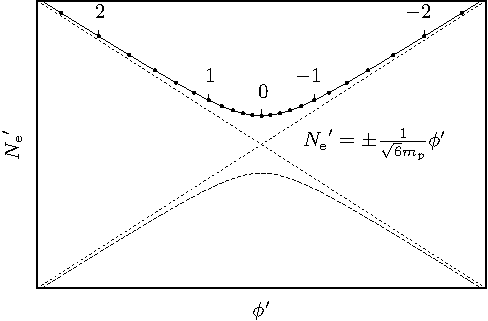
\includegraphics[width=\textwidth]{chapters/kinetic_dominance/figures/hyperbola}
  \caption{The constraint provided by the definition of \(\Nflat\) in Halliwell time. The dynamical variables \(\Nflatp\) and \(\prm \phi\) lie on a hyperbola according to~\protect\eqref{eqn:Friedmann_tau}. A natural parametrization uses a hyperbolic angle \(u\) detailed in~\protect\eqref{eqn:Ntrans} and~\protect\eqref{eqn:phitrans}. Note that only the upper half is parametrized, as the lower half of the hyperbola suggests a collapsing universe \((\Nflatp\propto H\propto\dot{a}<0)\). The points corresponding to \(u\in\{-2,-1,0,1,2\}\) have been labeled to guide the eye.}\label{fig:figure_hyperbola}
\end{figure}
%
Applying the transformation above to the Halliwell-time evolution equations, we find that equation~\eqref{eqn:Friedmann_tau} is trivially satisfied, and equation~\eqref{eqn:Raychaudhuri_tau} takes the form:
%
\begin{equation}
  \frac{\Nflatp}{\prm{N}} \frac{\m}{\sqrt{6}}
  \left(\frac{\sqrt{2}}{\sinh u} \frac{\d{u}}{\d{\tau}} 
  - \frac{1}{\tanh u} \frac{\d{}}{\d{\phi}}\log V\right) 
  = -1.
  \label{eqn:master_tau}
\end{equation}
%

\subsection{Hamilton-Jacobi representation}
\label{sec:Hamilton-Jacobi_representations}
We reformulate the equation using the Hamilton-Jacobi representation; instead of considering the variables as functions of time \(\tau\), one uses the field \(\phi\) as the independent variable. Since we are considering universes with a monotonic inflaton \((\dot{\phi}\ne 0)\), the transformation from \(t\) to \(\phi\) is monotonic, and hence so too is that from \(\tau\) to \(\phi\).

One can switch to the Hamilton-Jacobi representation by changing the variables in the derivatives using the relation:
%
\begin{equation}
  \difrac{}{\tau}
  =
  \difrac{\phi}{\tau}\difrac{}{\phi}
  =
  \prm\phi\difrac{}{\phi}
  =
  -\sqrt{2}\sinh u \difrac{}{\phi},
  \label{eqn:tautrans}
\end{equation}
%
which on applying to equation~\eqref{eqn:master_tau} yields:
%
\begin{equation}
  \m\frac{\Nflatp}{\prm{N}} \sqrt{\frac{2}{3}}
  \left(\frac{\d{u}}{\d{\phi}} 
  + \frac{1}{2\tanh u} \frac{\d{}}{\d{\phi}}\log V\right) 
  = 
  1.
  \label{eqn:master_phi}
\end{equation}
%
We now  rescale the \(\phi\) field into a new field \(\psi\) via the relation:
%
\begin{equation}
  \frac{\d{}}{\d{\psi}} 
  = 
  \m\frac{\Nflatp}{\prm{N}}\sqrt{\frac{2}{3}}\frac{\d{}}{\d{\phi}}.
\end{equation}
%
More explicitly, \(\psi\) is defined up to a constant by the monotonic transformation:
%
\begin{equation}
  \frac{\d{\psi}}{\d{\phi}} 
  = 
  \sqrt{\frac{3}{2}}\frac{\prm{N}}{\m\Nflatp} 
  \quad
  \Leftrightarrow\quad \psi 
  = 
  \sqrt{\frac{3}{2}}\frac{1}{\m}\int^\phi 
  \frac{\prm{N}}{\Nflatp}\:d\phi,
  \label{eqn:psi_by_phi}
\end{equation}
%
and this relationship is well defined since:
%
\begin{equation}
	\frac{\prm{N}}{\Nflatp} = \frac{H}{\Hflat} \ge 0.
\end{equation}
%
This rescaling absorbs all of the dependence on \(\prm N\) and thus \(\{\rho_i\}\) via~\eqref{eqn:N_H_relation} into the definition of \(\psi\). Under the transformation~\eqref{eqn:psi_by_phi}, the master equation~\eqref{eqn:master_phi} takes the form:
%
\begin{equation}
  \frac{\d{u}}{\d{\psi}}  
  = 
  1-\frac{1}{\tanh u} \frac{\d{}}{\d{\psi}}\log \sqrt V.
\end{equation}
%
We have transformed the evolution equations~\eqref{eqn:Raychaudhuri_mod}--\eqref{eqn:Klein_Gordon_mod} into a single ``master equation'' in one variable, where all of the potential dependence is kept in a single term.

We may rearrange this slightly by making the monotonic transformation:
%
\begin{equation}
  u\mapsto y = \log\cosh(u), 
  \label{eqn:y_def}
\end{equation}
%
under which the master equation takes the form:
%
\begin{equation}
  \frac{\d{y}}{\d{\psi}} = \sqrt{1-e^{-2y}} - \frac{\d{}}{\d{\psi}}\log \sqrt V.
  \label{eqn:master_eq}
\end{equation}
%

\subsection{Interpreting the master equation}
\label{sec:interpreting_the_master_equation}

We now prove kinetic dominance by considering the asymptotics of the master equation~\eqref{eqn:master_eq} in the limit \(a\rightarrow0\). We prove that there is at most a single solution \(f(\psi)\) which is finite, with all of the rest diverging as \(a\rightarrow0\). We finish by showing that a diverging solution \(y(\psi)\) of the master equation is equivalent to kinetic dominance.

We begin by examining the behaviour of \(\psi\) as \(a\rightarrow0\). Through elementary derivative transformations with the chain rule and the definitions of various variables, we find:
%
\begin{align}
  \frac{\prm\phi}{\Nflatp} 
  &=
  \frac{\prm\psi\frac{\d{\phi}}{\d{\psi}}}{\Nflatp}
  &\text{(chain rule)} 
  \nonumber
  \\
  &=
  \m\sqrt{\frac{2}{3}}\frac{\prm\psi}{\prm{N}}  
  &\text{(from equation \protect\ref{eqn:psi_by_phi})} 
  \nonumber
  \\
  &=
  \m\sqrt{\frac{2}{3}}\frac{\dot\psi}{\dot{N}}  
  &\text{(chain rule)} 
  \nonumber
  \\
  &=
  \m\sqrt{\frac{2}{3}}\frac{\d{\psi}}{\d{\log a}}
  &\text{(since \(H=\frac{\d{}}{\d{t}}\log a\))}.
  \label{eqn:div_psi}
\end{align}
%
Given the definition of Halliwell time~\eqref{eqn:tau_def}, on the left hand side of the above expression, we have \(\prm\phi = \dot\phi/\sqrt{V}\). Since \(\Nflatp>0\), and by assumption~\eqref{eqn:conditions} \({|\dot\phi|>\xi>0}\) we thus find that \(\psi\) is monotonic in \(a\).
The direction of the monotonicity of \(\psi\) can be found by considering the transformations we have made: %
\begin{equation}
  t
  \xrightarrow{\protect\eqref{eqn:tau_def}}
  \tau
  \xrightarrow{\protect\eqref{eqn:phitrans}}
  \phi
  \xrightarrow{\protect\eqref{eqn:psi_by_phi}}
  \psi.
\end{equation}
%
By considering the equations denoted above, one can see that \(\frac{\d{\tau}}{\d{t}}>0\), \(\frac{\d{\psi}}{\d{\phi}}>0\), and \(\frac{\d{\phi}}{\d{\tau}} = -\sqrt{2}\sinh u\). Thus as \(a\) and \(t\) decrease, one finds that if \(u>0\), then \(y>0\) by~\eqref{eqn:y_def} and thus \(\psi\) is monotonically {\em increasing}.\footnote{This explains the choice of sign in the parametrization~\protect\eqref{eqn:phitrans}.}
As we are considering universes where \(\dot{\phi}\ne 0\), this places the constraint that:
%
\begin{equation}
  u 
  = 
  \sinh^{-1}\left(\frac{\prm\phi}{\sqrt 2}\right) 
  = 
  \sinh^{-1}\left(\frac{\dot\phi}{\sqrt 2 V(\phi)}\right)
  \ne 
  0,
\end{equation}
%
and by~\eqref{eqn:y_def}, we find that \(y\ne0\) also.  The problem therefore breaks down into two cases: 
%
\begin{enumerate}
  \item \(y>0\) and \(\psi\) increasing
  \item \(y<0\) and \(\psi\) decreasing.
\end{enumerate}
%
We will consider the first case; the second may be treated in exactly the same way, with a couple of sign changes.  



Now, if the gradient of \(\psi\) with respect to \(\log a\) is strictly positive, then \(\psi\) diverges as \(a\to0\):
\begin{equation}
  \left| \frac{\d\psi}{\d\log a}\right|  > \varepsilon_\psi > 0 \qquad \Rightarrow \qquad |\psi| \to  \infty \quad\text{as}\quad a \to 0.
  \label{eqn:diverging_psi}
\end{equation}
From equations~\eqref{eqn:div_psi} and~\eqref{eqn:Friedmann_tau}, we can see the antecedent above may be equivalently stated as: 
\begin{equation}
  \frac{\dot\phi}{\sqrt{V}} > \varepsilon_\phi > 0 \qquad \Rightarrow \qquad |\psi| \to  \infty \quad\text{as}\quad a \to 0.
  \label{eqn:diverging_phi}
\end{equation}
Moreover, if \(\psi\) does not diverge, then since \({|\dot\phi|>\xi>0}\), then \(V\) must diverge. So we have two cases:
\begin{enumerate}
  \item \(\psi \to \psi_\smax\) and \(V\to\infty\)\label{itm:psimax}
  \item \(\psi \to \infty\)\label{itm:psidiv}
\end{enumerate}
We now show that in case~\ref{itm:psidiv} there is at most one {\em finite\/} solution \(y\) satisfying the master equation~\eqref{eqn:master_eq} while remaining positive (\(y>0\)), and that in case~\ref{itm:psimax}, there is no solution which remains positive.

\subsubsection{Case~\protect\ref{itm:psimax}}
We first show that if \(\psi\) does not diverge, but instead tends to some maximum value \(\psi_\smax\), then solutions to the master equation~\eqref{eqn:master_eq} cannot remain positive. Integrating the master equation~\eqref{eqn:master_eq} from some start point up to \(\psi_\smax\):
\begin{equation}
  y(\psi) = \int^{\psi_\smax} \sqrt{1-e^{-2y}} \d{\psi} - \log\sqrt{V} + c.
\end{equation}
Considering the right hand side, Given that the integrand is bounded, and that the integral is over a finite range, the first term remains finite. However, we know that in this case \(V\) and hence \(\log\sqrt V\) must diverge, hence the solution \(y\) must become negative as \(\psi\to\psi_\smax\). This behaviour is further examined in Section~\ref{sec:pathological_oscillations}. We may thus discount case~\protect\ref{itm:psimax}, since it is counter to our initial assumption~\eqref{eqn:conditions} of a steadily moving inflaton.


\subsubsection{Case~\protect\ref{itm:psidiv}}
We now show that there is at most one {\em finite\/} solution \(y\) satisfying the master equation~\eqref{eqn:master_eq} while remaining positive (\(y>0\)).

Let us assume that there exists a solution \(f(\psi)\) of~\eqref{eqn:master_eq} that is positive and finite (\(0<f<\fm\) for some finite \(\fm\)):
%
\begin{equation}
  \difrac{f}{\psi} = \sqrt{1-e^{-2f}} -\frac{\d{}}{\d{\psi}}\log \sqrt V.
  \label{eqn:master_eq_f}
\end{equation}
%
where:
%
\begin{equation}
  0<f(\psi)<\fm,
\end{equation}
%
and assume some initial condition on \(f\) at some finite value
\(\psi=\psiz\):
%
\begin{equation}
  f(\psiz)=\fz.
\end{equation}
%
Now consider a solution \(h(\psi)\) with some larger initial value:
%
\begin{equation}
  h(\psiz)=\hz>\fz.
\end{equation}
%
Since \(h\) is also a solution of the master equation~\eqref{eqn:master_eq} it satisfies:
%
\begin{equation}
  \difrac{h}{\psi} = \sqrt{1-e^{-2h}} -\frac{\d{}}{\d{\psi}}\log \sqrt V.
  \label{eqn:master_eq_h}
\end{equation}
%
Taking the difference of~\eqref{eqn:master_eq_f} and~\eqref{eqn:master_eq_h} gives:
%
\begin{equation}
  \frac{\d{}}{\d{\psi}}\left(h-f\right)
  = 
  \sqrt{1-e^{-2h}}-\sqrt{1-e^{-2f}}
  \label{eqn:master_eq_diff}
\end{equation}
%
By a uniqueness theorem, discussed in Section~\ref{sec:uniqueness_theorem}, if \(h(\psiz)>f(\psiz)\), then \(h(\psi_1)>f(\psi_1)\) (for \(\psi_1\ne\psi_0\)). Therefore one can see from~\eqref{eqn:master_eq_diff} that the difference between \(h\) and \(f\) is monotonically increasing in any finite interval \([\psiz,\psi_1]\).  One can thus conclude that:
%
\begin{equation}
  h-f>\hz-\fz=\Delta_0>0
  \label{eqn:cosh_rel}
\end{equation}
%
where we have defined \(\Delta_0 = \hz-\fz\), and \(h\) and \(f\) are evaluated at the end of the interval \(\psi_1\). Since \(h>\Delta_0+f\), it is easy to see using~\eqref{eqn:master_eq_diff} that:
%
\begin{equation}
  \frac{\d{}}{\d{\psi}}\left(h-f\right)
  > 
  \sqrt{1-e^{-2(f+\Delta_0)}}-\sqrt{1-e^{-2f}}
\end{equation}
%
This is a monotonically decreasing function of \(f\), and hence attains its minimum at \(\fm\); thus,
%
\begin{equation}
  \frac{\d{}}{\d{\psi}}\left(h-f\right)
  > 
  \sqrt{1-e^{-2(\fm+\Delta_0)}}-\sqrt{1-e^{-2\fm}} 
  >
  0.
\end{equation}
%
The difference between \(h\) and \(f\) is therefore monotonically increasing at a rate greater than some positive number. Since \(f\) is positive, it is bounded below and as \(\psi_1\) is made arbitrarily large, \(h\) grows without bound.

%
\begin{figure}[tp]
  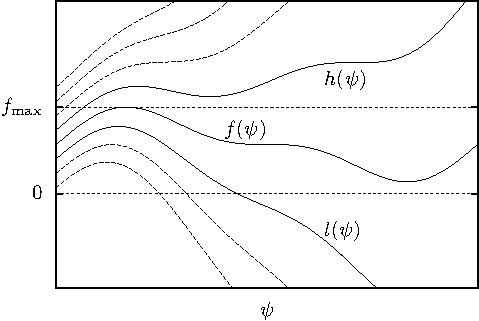
\includegraphics[width=\textwidth]{chapters/kinetic_dominance/figures/uschem}
  \caption{In general there is at most a single solution \(f(\psi)\) to the master equation~\protect\eqref{eqn:master_eq} that is positive and finite \(0<f(\psi)<\fm\). Any solution \(h(\psi)\) that begins higher than \(f(\psi)\) must diverge. Consequently, any solution \(l(\psi)\) that begins lower than \(f(\psi)\) cannot remain above \(0\). If it were able to, then \(l(\psi)\) would also be another finite solution lying between \(0\) and some \(l_\smax\). By the previous argument, this would mean \(f\) could not be finite, contradicting our initial assumption.\label{fig:figure_uschem}}
\end{figure}
%
We therefore find ourselves in a situation demonstrated in Figure~\ref{fig:figure_uschem}. For any given potential \(V(\phi)\), there is at most a single solution \(f(\psi)\) that is finite and positive [\(0<f(\psi)<\fm\)]: any solution that is larger than \(f(\psi)\) at some point \(\psi=\psiz\) diverges as \(\psi\to\infty\) (\(a\to0\)). Further, any solution \(l(\psi)\) that starts out less than \(f(\psi)\) must fall to a value less than \(0\).  If \(l(\psi)\) did not fall below \(0\), but were another example of a finite positive solution, then by the argument above, this would imply \(f(\psi)>l(\psi)\) must diverge, contradicting our initial assumptions on \(f(\psi)\).

One therefore expects universes with a steadily moving inflaton to have a generically diverging \(y\) as \(a\to0\), except perhaps for a single special case for a given potential \(V(\phi)\).  The consequences of a generically divergent \(y\) shall now be examined.  If \(y\) diverges, then so does \(u\) by equation~\eqref{eqn:y_def}. If \(u\) diverges, then we find that \(\prm \phi\) diverges by~\eqref{eqn:phitrans}:
%
\begin{equation}
  \frac{\d{\phi}}{\d{\tau}}=\prm{\phi} 
  = 
  -\sqrt{2}\sinh u\rightarrow -\infty.
\end{equation}
%
Converting back from Halliwell time to cosmic time using equation~\eqref{eqn:tau_def} shows:
%
\begin{equation}
  \prm{\phi}^2 
  = 
  \frac{\dot{\phi}^2}{V(\phi)}
\end{equation}
%
One can thus see that the divergence of \(y\), \(u\) and \(\prm \phi\) therefore requires that:
%
\begin{equation}
  \lim\limits_{y\to\pm\infty} \frac{\dot\phi^2}{V(\phi)}
  =
  \lim\limits_{a\to 0} \frac{\dot\phi^2}{V(\phi)} = \infty,
  \label{eqn:kdfinal}
\end{equation}
%
which is equivalent to saying that \(\dot{\phi}^2\gg V(\phi)\) as
\(a\to0\). The early universe is generically kinetically dominated.

\section{Consequences of kinetic dominance}
\label{sec:consequences_of_kinetic_dominance}

The condition \(\dot\phi^2\gg V(\phi)\) for kinetic dominance allows one to derive several results. First, the kinetic energy of the inflaton dominates over the other fluids as \(a\to 0\), allowing us at early times to neglect any additional effects such as curvature, radiation, matter or a cosmological constant. Second, the universe emerges from an initial singularity at a finite coordinate time, which may be taken as \(t=0\). Finally, one is able to determine exact analytic expressions for the solutions in coordinate or conformal time for each of the cases where curvature, radiation, matter or a cosmological constant are present.


\subsection{Dominance of \(\dot{\phi}^2\) over other fluids}
\label{sec:dominance_fluids}
In the limit that \(a\to 0\), the auxiliary fluid with the largest value of \(w\) dominates over all of the others. Along with kinetic dominance, we can therefore assume that the acceleration~\eqref{eqn:Raychaudhuri_mod} and Friedmann~\eqref{eqn:Friedmann_mod} equations take the form:
%
\begin{align}
  \dot{H}+H^2 
  &= 
  -\frac{\dot{\phi}^2}{3\m^2} - \frac{1}{6\m^2}(1+3w)\rho_w
  \label{eqn:Ray_KD_eq_rho}
  \\
  H^2 
  &= 
  \frac{\dot{\phi}^2}{6\m^2} +  \frac{1}{3\m^2}\rho_w,
  \label{eqn:Friedmann_KD_eq_rho}
\end{align}
  %
where \(\rho_w\) is the density of the auxiliary fluid with the largest \(w\).  It is not difficult to show using equation~\eqref{eqn:rho_a},
along with \(H=\frac{\d{}}{\d{t}}\log a\) that these equations solve to give:
%
\begin{align}
  H^2 
  &= 
  \frac{1}{3\m^2}\left(\frac{\beta^2}{a^6} + \rho_w\right) 
  \label{eqn:H_of_a_1}
  \\
  \dot{\phi}^2 
  &= 
  2\frac{\beta^2}{a^6} 
  \label{eqn:dotphi_of_a_1}
\end{align}
%
where \(\beta\) is an integration constant. From this, if \(w<1\) then as
\(a\to 0\), one finds:
%
\begin{equation}
  \dot{\phi}^2 \propto a^{-6} 
  \gg
  \rho_w \propto a^{-3(1+w)}.
  \label{eqn:dotphidom}
\end{equation}
%
Thus, the kinetic term of the inflaton dominates over all other fluids with \(w<1\).




Historically, inflationary potentials were considered in the context of grand unified theories \citep{PhysRevLett.48.1220,linde_1982} which resulted in an effective potential \(V(\phi,T)\) depending on the value of the field \(\phi\) and a temperature.  This was then developed \citep{1995PhRvL..74.1912B,PhysRevLett.75.3218} into a theory in which the inflaton remains in thermal equilibrium with an auxiliary radiation fluid.

More recent work \citep{2007PhRvD..76f3512P} typically assumes that the inflaton is decoupled from the auxiliary fluids in the preinflationary phase, and that the universe is {\em radiation dominated\/} at this early stage. Given the above result~\eqref{eqn:dotphidom}, such assumptions may now need revisiting.



\subsection{Finite time singularity}

Since \(H = \dot{a}/a\), we can express the coordinate time \(t\) as an integral: 
%
\begin{equation}
  t = \int \frac{\d{a}}{aH}.
\end{equation}
%
From equation~\eqref{eqn:H_of_a_1}, one can see that \({(aH)}^{-1}\) is finite as \(a\to0\). By the above integral, this shows that the universe emerges at a finite time in the past, which can be taken as \(t=0\).  Moreover, from~\eqref{eqn:dotphidom}, the (dominant) energy density of the universe scales as \(a^{-6}\) as \(a \to 0\), showing that \(t=0\) is a singularity.

\subsection{Analytic solutions for the kinetically dominated universe} 
If one considers the solutions of the acceleration and Friedmann equations~\eqref{eqn:Raychaudhuri_mod} and~\eqref{eqn:Friedmann_mod} in the limit that \(a\to0\), then one can neglect the potential term \(V(\phi)\) as it is suppressed by \(\dot{\phi}^2\). In addition, the other fluid terms are negligible in comparison to the term with the largest \(w\).  When these considerations are taken into account, the evolution equations take the form shown in~\eqref{eqn:Ray_KD_eq_rho} and~\eqref{eqn:Friedmann_KD_eq_rho}. One can find solutions for \(\phi(a),H(a)\) and \(\rho_w(a)\) parametrically in terms of \(a\).  In addition, one can find coordinate time \(t(a)\) in terms of \(a\) using the relation:
%
\begin{equation}
  t = \int \frac{\d{a}}{aH(a)}.
\end{equation}
%
Conformal time \(\eta\) is defined by the equation \(\dot{\eta} =
a^{-1}\), and can be found in terms of \(a\) using:
%
\begin{equation}
  \eta = \int \frac{\d{a}}{a^2H(a)}.
\end{equation}
%
The solutions are:
%
\begin{align}
  \rho_w(a) 
  &\propto 
  a^{-3(1+w)} 
  \\
  H{(a)}^2 
  &= 
  \frac{1}{3\m^2}\left(\frac{\beta^2}{a^6} + \rho_w\right)  
  \label{eqn:H_of_a}
  \\
  \dot{\phi}{(a)}^2
  &=
  2\frac{\beta^2}{a^6} 
  \label{eqn:dotphi_of_a}
  \\
  \phi(a)
  &=
  c + \pm
  \sqrt{\frac{2}{3}}\frac{\m}{1-w} \ln \left[ 
  \frac 
  {{a}^{3(1-w)}}
  {{\left(\sqrt{1+\frac{\rho_w{a}^{6}}{\beta^2}}+1\right)}^2} 
  \right]  
  \label{eqn:phi_of_a}
  \\
  t(a)
  &=
  a^3 \frac{\m\sqrt{3}}{3\beta} 
  \:\: 
  {_2F_1}(
  \frac{1}{2},
  \frac{1}{1-w};
  \frac{2-w}{1-w},
  -\frac{a^6\rho_w}{\beta^2}
  ) 
  \label{eqn:t_of_a}
  \\
  \eta(a) 
  &= 
  a^2 \frac{\m\sqrt{3}}{2\beta}
  \:\: 
  {_2F_1}(
  \frac{1}{2},
  \frac{2}{3(1-w)};
  \frac{5-3w}{3(1-w)},
  -\frac{a^6\rho_w}{\beta^2}
  ),
  \label{eqn:eta_of_a}
\end{align}
%
where \(\beta\) and \(c\) are constants of integration which will be redefined shortly. We have chosen \(t,\eta\) such that \(a\to0\) as \(t,\eta \to 0\).


For specific values of \(w\), the hypergeometric functions \(_2F_1\) take simple forms. If \(w=-1\) or \(0\), then equation~\eqref{eqn:t_of_a} is expressible in closed form, in terms of trigonometric and algebraic functions in \(a\) respectively. If \(w=-1/3\) or \(1/3\), then~\eqref{eqn:eta_of_a} may be expressed in closed form. In each of these cases, these equations are invertible giving an expression for \(a(t)\) or \(a(\eta)\).  We note that, except for the case \(w=-1/3\), the solutions~\eqref{eqn:H_of_a}--\eqref{eqn:eta_of_a} correspond to a spatially flat universe.

We shall examine each of the above cases in turn, after first looking at the case in which there are no auxiliary fields, \(\rho_w=0\).  In so doing, it will prove useful to define the functions:
%
\begin{equation}
  \begin{array}{rr}
    S_k(x),&S_k^{-1}(x)
    \\ 
    C_k(x),&C_k^{-1}(x)
    \\ 
    T_k(x),&T_k^{-1}(x)
    \\
  \end{array}
  =
  \left\{
%
  \begin{array}{rl}
%
    \begin{array}{rr}
      \sin(x),&\arcsin(x)
      \\ 
      \cos(x),&\arccos(x)
      \\ 
      \tan(x),&\arctan(x)
      \\
    \end{array}
%
    &: k>0 \\
%
    \begin{array}{rr}
      x,&x
      \\ 
      1,&1
      \\ 
      x,&x
      \\
    \end{array}
%
    &: k=0 \\
%
    \begin{array}{rr}
      \sinh(x),&\arcsinh(x)
      \\ 
      \cosh(x),&\arccosh(x)
      \\ 
      \tanh(x),&\arctanh(x)
      \\
    \end{array}
%
    &: k<0
  \end{array}
%
  \right. 
\end{equation}
%

\subsubsection{No auxiliary fields, \(\rho_w=0\)}
If \(\rho_w=0\), then equation~\eqref{eqn:t_of_a} becomes:
%
\begin{equation}
  t = a^3 \frac{\m\sqrt{3}}{3\beta}.
\end{equation}
%
One can rearrange this to find \(a\) as a function of \(t\),
%
\begin{equation}
  a(t)
  =
  t^{1/3} {\left(\frac{3\beta}{\m\sqrt{3}}\right)}^{1/3},
  \label{eqn:a_of_t_beta_flat}
\end{equation}
%
and then substitute this into equations~\eqref{eqn:H_of_a} and~\eqref{eqn:dotphi_of_a} to find:
%
\begin{align}
  H(t) 
  &= 
  \frac{1}{3t}, 
  \label{eqn:H_of_t_flat} 
  \\
  \dot{\phi}(t) 
  &= 
  \pm\sqrt{\frac{2}{3}}\frac{\m}{t}.
  \label{eqn:dotphi_of_t_flat}
\end{align}
%
The latter integrates to give:
%
\begin{equation}
  \phi(t) 
  = 
  \phip \pm\sqrt{\frac{2}{3}}\m\log\left(\frac{t}{\tp}\right),  
  \label{eqn:phi_of_t_flat}
\end{equation}
%
where \(\phip\) is an integration constant chosen such that \(\phi(\tp)=\phip\), where \(\tp\) is some time. It is more appropriate to redefine the integration constant \(\beta\) as:
%
\begin{equation}
  \beta 
  \equiv 
  \frac{\Rp^3\m}{\tp\sqrt{3}}, 
  \label{eqn:beta_def}
\end{equation}
%
since then, equation~\eqref{eqn:a_of_t_beta_flat} for \(a(t)\) becomes:
%
\begin{equation}
  a(t) 
  = 
  \Rp {\left(\frac{t}{\tp}\right)}^{1/3},
  \label{eqn:a_of_t_flat}
\end{equation}
%
which is more in keeping with equation~\eqref{eqn:phi_of_t_flat}.  

For this case, one can also obtain analytical solutions in terms of conformal time.  If \(\rho_w=0\) and \(\beta\) is defined by~\eqref{eqn:beta_def}, equation~\eqref{eqn:eta_of_a} becomes:
%
\begin{equation}
  \eta(t) 
  = 
  a^2 \frac{\m\sqrt{3}}{2\beta}
  =
  \frac{3\tp}{2\Rp^3}a^2.
  \label{eqn:eta_of_t}
\end{equation}
%
Using equation~\eqref{eqn:a_of_t_flat}, we can show:
%
\begin{equation}
  \eta
  =
  \etap{\left(\frac{t}{\tp}\right)}^{2/3},
\end{equation}
%
where we have defined \(\etap\) as:
%
\begin{equation}
  \etap
  =
  \frac{3\tp}{2\Rp}.
  \label{eqn:etap_eq}
\end{equation}
%
Now we have \(\eta(t)\) in equation~\eqref{eqn:eta_of_t}, we can change equations~\eqref{eqn:H_of_t_flat},~\eqref{eqn:dotphi_of_t_flat},~\eqref{eqn:phi_of_t_flat} and~\eqref{eqn:a_of_t_flat} to:
%
\begin{align}
  a(\eta)
  &=
  \Rp {\left(\frac{\eta}{\etap}\right)}^{1/2},
  \\
  H(\eta)
  &=
  \frac{1}{3\tp}{\left(\frac{\eta}{\etap}\right)}^{-3/2},
  \\
  \dot{\phi}(\eta)
  &=
  \pm\sqrt{\frac{2}{3}}
  \frac{\m}{\tp}{\left(\frac{\eta}{\etap}\right)}^{-3/2},
  \\
  \phi(\eta)
  &=
  \phip \pm\sqrt{\frac{3}{2}}\m\log\left(\frac{\eta}{\etap}\right). 
  \label{eqn:phi_flat}
\end{align}
%

It should be noted that since \(\dot{\phi}^2 \gg \rho_w\) at sufficiently early times, all solutions reduce to the above forms for small enough \(t\) or \(\eta\). We can thus fix the form of solutions with nonzero \(\rho_w\) by matching onto the above solutions for sufficiently small \(t\) or \(\eta\).  

\subsubsection{Dark energy, \(w=-1\)}
For dark energy in the form of a cosmological constant, we find that the energy density in standard notation is:
%
\begin{equation}
  \rho_w = \m^2\Lambda.
\end{equation}
%
For \(w=-1\), equation~\eqref{eqn:t_of_a} is expressible in terms of trigonometric functions, and may be rearranged to express the scale factor \(a\) in terms of coordinate time. Once \(a(t)\) is obtained, the remaining equations~\eqref{eqn:H_of_a},~\eqref{eqn:dotphi_of_a} and~\eqref{eqn:phi_of_a} can be used to express the rest of the variables in terms of \(t\). Using our definition of \(\beta\) [equation \nolinebreak\ref{eqn:beta_def}], and defining the new time scale,
%
\begin{equation}
  \tL = \frac{1}{\sqrt{3\Lambda}},
  \label{eqn:tl}
\end{equation}
%
the solutions are:
%
\begin{align}
  a(t)
  &=
  \Rp{\left[{\frac {S_{-\Lambda}(t/\tL)}{\tp/\tL}}\right]}^{1/3},
  \\
  H(t)
  &=
  \frac{1}{3\tL}\frac{1}{T_{-\Lambda}(t/\tL)},
  \\
  \dot{\phi}(t)
  &=
  \sqrt{\frac{2}{3}}\frac{\m}{\tL}\frac{1}{S_{-\Lambda}(t/\tL)},
  \\
  \phi(t)
  &=
  \phip \pm \sqrt{\frac{2}{3}}\m
  \log\left[
  \frac{\tL}{\tp} 
  \frac 
  {2\: S_{-\Lambda} \left( t/\tL \right) }
  {1 + C_{-\Lambda} \left( t/\tL \right)}  
  \right].
\end{align}
%

\subsubsection{Spatial curvature, \(w=-1/3\)}
Spatial curvature is equivalent to a fluid with equation-of-state parameter \(w=-1/3\) and density:
%
\begin{equation}
  \rho_w = -3\m^2\frac{\kappa}{a^{2}}.
\end{equation}
%
For \(w=-1/3\), equation~\eqref{eqn:eta_of_a} is expressible in terms of trigonometric functions, and may be rearranged to express the scale factor \(a\) in terms of conformal time. Once \(a(\eta)\) is obtained, the remaining equations~\eqref{eqn:H_of_a},~\eqref{eqn:dotphi_of_a} and~\eqref{eqn:phi_of_a} can be used to express the rest of the variables in terms of \(\eta\). Using our definitions of \(\beta\) [equation \nolinebreak\ref{eqn:beta_def}] and \(\etap\) [equation \nolinebreak\ref{eqn:etap_eq}], and defining the new time scale,
%
\begin{equation}
  \etak = \frac{1}{2\sqrt{\kappa}},
  \label{eqn:etak}
\end{equation}
%
the solutions are:
%
\begin{align}
  a(\eta)
  &=
  \Rp{\left[
  \frac
  {S_\kappa\left(\eta/\etak\right)}
  {\etap/\etak} \right]}^{1/2},
  \\
  H(\eta)
  &=
  \frac{1}{3\tp}
  \frac{{(\etap/\etak)}^{3/2}}
  {T_\kappa(\eta/\etak)\sqrt{S_\kappa(\eta/\etak)}}, 
  \\
  \dot{\phi}(\eta)
  &=
  \pm\sqrt{\frac{2}{3}}
  \frac{\m}{\tp}
  {\left[
  \frac
  {\etap/\etak}
  {S_{\kappa}(\eta/\etak)}
  \right]}^{3/2},
  \\
  \phi(\eta) 
  &=
  \phip \pm \sqrt{\frac{3}{2}}\m\log  \left[
  \frac{\etak}{\etap} 
  \frac{2\:S_{\kappa}\left(\eta/\etak \right) }
  {1 + C_{\kappa} \left( \eta/\etak \right)   }  
  \right]. 
\end{align}
%



\subsubsection{Matter, \(w=0\)}
For matter with zero pressure, one has \(w=0\) and so:
%
\begin{equation}
  \rho_w = \rhomp{\left(\frac{a}{\Rp}\right)}^{-3},
\end{equation}
%
where \(\rhomp\) is an integration constant, labeling the energy density of matter at the epoch \(\Rp\).  For \(w=0\), equation~\eqref{eqn:t_of_a} is expressible as an algebraic function, and may be rearranged to express the scale factor \(a\) in terms of coordinate time. Once \(a(t)\) is obtained, the remaining equations~\eqref{eqn:H_of_a},~\eqref{eqn:dotphi_of_a}~\&~\eqref{eqn:phi_of_a} can be used to express the rest of the variables in terms of \(t\). Using our definition of \(\beta\) (equation~\ref{eqn:beta_def}), and defining the new time scale,
%
\begin{equation}
  \tm = \frac{4\m^2}{3\tp\rhomp },
  \label{eqn:tm}
\end{equation}
%.
the solutions are:
%
\begin{align}
  a(t)
  &=
  \Rp{\left(\frac{t}{\tp}\right)}^{1/3}
  {\left(1+\frac{t}{\tm}\right)}^{1/3} ,
  \\
  H(t) &= 
  \frac{1+2\frac{t}{\tm}}{3t{{\left( 1+\frac{t}{\tm} \right) }}},
  \\
  \dot{\phi}(t) &= 
  \pm\sqrt{\frac{2}{3}}\m
  \frac{1}
  {t \left( 1+\frac{t}{\tm} \right) },
  \\
  \phi(t) &=
  \phip \pm \sqrt{\frac{2}{3}}\m \log\left[  
  \left(\frac{t}{\tp}\right) 
  \frac {1}{1+\frac{t}{\tm}}  
  \right].
\end{align}
%




\subsubsection{Radiation, \(w=1/3\)}

For radiation one has \(w=1/3\), and so:
%
\begin{equation}
  \rho_w = \rhorp{\left(\frac{a}{\Rp}\right)}^{-4},
\end{equation}
%
where \(\rhorp\) is an integration constant, labeling the energy density of matter at the epoch \(\Rp\).  For \(w=1/3\), equation~\eqref{eqn:eta_of_a} is expressible as an algebraic function, and may be rearranged to express the scale factor \(a\) in terms of coordinate time. Once \(a(\eta)\) is obtained, the remaining equations~\eqref{eqn:H_of_a},~\eqref{eqn:dotphi_of_a} and~\eqref{eqn:phi_of_a} can be used to express the rest of the variables in terms of \(\eta\). Using our definition of \(\beta\)~\ref{eqn:beta_def}, and \(\etap\)~\ref{eqn:etap_eq}, and defining the new time scale,
%
\begin{equation}
  \etar = \frac{3\m^2}{\Rp^2\etap\rhomp}.
  \label{eqn:etar}
\end{equation}
%
the solutions are:
%
\begin{align}
  a(\eta)
  &=
  \Rp{\left(\frac{\eta}{\etap}\right)}^{1/2}
  {\left({1+\frac{\eta}{\etar}}\right)}^{1/2},
  \\
  H(\eta) 
  &= 
  \frac{1}{3\tp}{\left(\frac{\eta}{\etap}\right)}^{-3/2}
  \frac{1+ 2\frac{\eta}{\etar}}
  {{\left(1+ \frac{\eta}{\etar}\right)}^{3/2}},
  \\
  \dot{\phi}(\eta) 
  &=
  \sqrt{\frac{2}{3}}\frac{\m}{\tp}
  {\left(\frac{\eta}{\etap}\right)}^{-3/2}
  \frac{1}{{\left(1+ \frac{\eta}{\etar}\right)}^{3/2}},
  \\ 
  \phi(\eta) 
  &=
  \phip+\sqrt {\frac{3}{2}}\m\log  
  \left[
  \left(\frac{\eta}{\etap}\right)
  \frac {1}{\left(1+ \frac{\eta}{\etar}\right)} 
  \right] 
\end{align}
%

\subsection{The constants of integration}
\label{sec:constants}
In the previous section, several constants arose, which we shall now review. For the system of equations~\eqref{eqn:Ray_KD_eq_rho}--\eqref{eqn:Friedmann_KD_eq_rho}, one would expect four constants of integration. The first is chosen by setting \(a=0\) at \(t=0\). For the case \(\rho_w=0\), the second and third are chosen by choosing a later time \(\tp>0\) and fixing:
%
\begin{align}
  \phi(\tp) &= \phip, \nonumber\\
  a(\tp) &= \Rp. \nonumber
\end{align}
%
We can also determine conformal time in this case, which involved defining a new constant \(\etap\) in terms of \(\Rp\) and \(\phip\) via equation~\eqref{eqn:etap_eq}, and the solutions may be determined in conformal time. For the remaining cases, there is an additional integration constant determined by the value of \(\rho_w\) when the scale factor is \(\Rp\). The solutions for these cases are then determined by matching them onto the case \(\rho_w=0\) at early times.

In addition, we defined a relevant time scale for each of the \(\rho_w \neq 0\) cases: \(\tL\), \(\etak\), \(\tm\), \(\etar\). These are expressed in terms of the previous integration constants in equations~\eqref{eqn:tl},~\eqref{eqn:etak},~\eqref{eqn:tm} and~\eqref{eqn:etar}. If one chooses \(\tp\) or \(\etap\) to be much less than this second time scale, then the universe is in a fully kinetically dominated regime at \(\tp\), \(\etap\), with solutions very close to the \(\rho_w=0\) case. When \(\eta\) is of the order of the second time scale, then the effects of the universe's (dominant) additional component can be seen.

Although we have determined these equations in terms of three integration constants, there are in fact only two.  The evolution equations~\eqref{eqn:Raychaudhuri_mod}~\&~\eqref{eqn:Friedmann_mod} possess a two-parameter symmetry corresponding to a rescaling of \(a\) and \(t\). More precisely, the form of the equations does not change under the transformation:
%
\begin{equation}
  a\mapsto\alpha a, 
  \qquad 
  t \mapsto\sigma^{-1}t,
\end{equation}
%
provided that \(\rho_i\) and the potential transform as:
%
\begin{equation}
  \rho_i \mapsto \alpha^{3(1+w_i)}\sigma^2\rho_i, 
  \qquad
  V(\phi) \mapsto \sigma^2 V(\phi)
\end{equation}
%
This symmetry can be used effectively to remove some of the remaining integration constants. In practice this means that one may set \(\tp=1\) to be the Planck time and the scale factor \(a(\tp)=\Rp=1\). Usually one takes the scale factor to be unity at the present epoch \(a_0\equiv a(t_0)=1\), but this requirement is complicated by the uncertainties of reheating, so we do not follow that convention here. One may ``physically'' interpret \(\phip\) as the value of the field at \(t=t_p\).  This requires extrapolating the classical equations far beyond their validity, so it is more of a mnemonic aid than a physical interpretation.  As we will see below, \(\phip\) controls the total number of \(e\)-folds of inflation.













\section{Kinetic dominance in action}
\label{sec:Kinetic_dominance_in_action}

We shall now demonstrate the utility of kinetic initial conditions in the analysis of inflationary models. Even without integrating the evolution equations for \(H(t)\) and \(\phi(t)\), one sees that the basic scenario entails the universe emerging from an initial singularity at \(t=0\) in a regime where the kinetic energy of the inflaton dominates its potential energy along with any curvature or additional fluids.  The evolution of \(H(t)\) and \(\phi(t)\) in this regime are given by~\eqref{eqn:H_of_t_flat} and~\eqref{eqn:phi_of_t_flat} at sufficiently early times.  \(H(t)\) and \(|\phi(t)|\) and their time derivatives decrease during this period of kinetic dominance, which concludes when there is approximate equipartition \(\dot{\phi}^2 \sim V(\phi)\) between the kinetic and potential energies of the inflaton.  This marks the onset of a (typically brief) period of fast-roll inflation \citep{Linde:2001}, which must eventually become slow-roll inflation, with \(\dot{\phi}^2 \ll V(\phi)\), since the latter is a generic attractor solution for inflation models \citep{belinsky_inflationary_1985}.  We will see that integration of the equations of motion in some illustrative cases does indeed verify these expectations.

For simplicity we shall work in the case with no other additional fields, \(\rho_w=0\), although our methods apply equally well to more complicated solutions. After discussing the validity of the initial conditions and numerical techniques, we shall consider two forms of potential: polynomial and exponential.

\subsection{Initial conditions and scaling}

For \(\rho_w=0\) the universe is spatially flat and contains only the inflaton field. The evolution equations then take the form:
%
\begin{align}
  H^2 
  &= 
  \frac{1}{3\m^2}
  \left(\frac{1}{2}\dot{\phi}^2 + V(\phi) + \sum_i\rho_i\right),
  \label{eqn:Friedmann_eq} 
  \\
  0
  &= 
  \ddot{\phi} +3\dot{\phi}^2H + V^\prime(\phi).
  \label{eqn:Motion_eq_Scalar}
\end{align}
%
The general solution to the evolution equations has the asymptotic form given in equations~\eqref{eqn:H_of_t_flat} and~\eqref{eqn:phi_of_t_flat}. As discussed in Section~\ref{sec:constants}, we may choose \(\tp=1\) to be the Planck time. Given this, we set the initial conditions at an initial time \(\ti\) as:
%
\begin{align}
  \phi(\ti) \equiv \phii
  &= 
  \phip - \sqrt{\frac{2}{3}}\m\log \ti, 
  \label{eqn:phi_ic}
  \\
  \dot\phi(\ti) 
  \equiv 
  \phidi
  &= 
  -\sqrt{\frac{2}{3}}\frac{\m}{\ti}, 
  \label{eqn:phid_ic}
  \\
  H(\ti) 
  \equiv 
  \Hi
  &= 
  \frac{1}{3\ti}. 
  \label{eqn:H_ic}
\end{align}
There is a single constant of integration \(\phip\), which directly controls the number of \(e\)-folds during inflation. The number of \(e\)-folds \(N_*\) between the pivot scale \(k_*\) and the end of inflation is typically \(50\)--\(60\) \citep{planck_collaboration_planck_2013-1}. For the rest of this chapter \(\phip\) will be chosen so that the total number of \(e\)-folds \(N_\mathrm{tot}=55\). This will be discussed in greater detail in Section~\ref{sec:powspec}.

Throughout this chapter we work in the classical regime. In order for the conditions above to be valid, the initial conditions must be set at a time greater than the Planck time, \(\ti >\tp=1\), but within the kinetic dominated regime, for which \(V(\phii) \ll \phidi^2\). Setting \(\ti=\tp=1\) in the above, one sees that kinetic dominance will endure beyond the Planck time provided:
%
\begin{equation}
  V(\phip) \ll \m^2.
\end{equation}
%
The above requirement typically holds for potentials that give physically reasonable inflation models. For example, in the case of a free inflaton with mass \(m\), one has \[ V(\phi) = \frac{1}{2}m^2 \phi^2.\] In order to generate the correct amplitude of curvature perturbations, the mass must be of the order \(m\sim10^{-5}\m\), whereas to generate the correct number of \(e\)-folds one requires \(\phip\bigO{10}\), in which case \(V(\phip) \sim 10^{-8} \m^2\).  Thus, there is no need to advocate trans-Planckian physics, since kinetic dominance lasts well beyond the Planck time, so one can set \(\ti \gg \tp\).


We note that the evolution equations~\eqref{eqn:Friedmann_eq}~\&~\eqref{eqn:Motion_eq_Scalar} are invariant under  the simultaneous rescaling of the time coordinate, Hubble parameter and inflaton potential:
%
\begin{align}
  t 
  &\longmapsto 
  \sigma^{-1}t,
  \\
  H 
  &\longmapsto 
  \sigma H,
  \\
  V(\phi) 
  &\longmapsto
  \sigma^2 V(\phi).
\end{align}
%
The advantage of this for numerical work is that a multiplicative scaling parameter from the potentials can be removed without loss of generality.


\subsection{Polynomial potentials}
\label{sec:section_polynomial_potentials}
We begin by analyzing examples of polynomial potentials of the form:
%
\begin{equation}
  \Vpol(\phi) = \mu^2\phi^n.
  \label{eqn:polpot}
\end{equation}
%
To obtain results we integrate the evolution equations~\eqref{eqn:Friedmann_eq}~\&~\eqref{eqn:Motion_eq_Scalar} numerically.  Our kinetic initial conditions are chosen using equation~\eqref{eqn:phi_ic}--\eqref{eqn:H_ic} with an initial time \(\ti\) small enough such that the inflaton is in the kinetic regime \(V(\phii)\ll\dot{\phii}^2\). For the purposes of numerics the scaling parameter \(\mu\) can be removed by rescaling the time coordinate (setting \(\sigma=\mu^{-1}\)). \(\phip\) is set by requiring that there be \(55\) \(e\)-folds during inflation.

%
\begin{figure}[tp]
  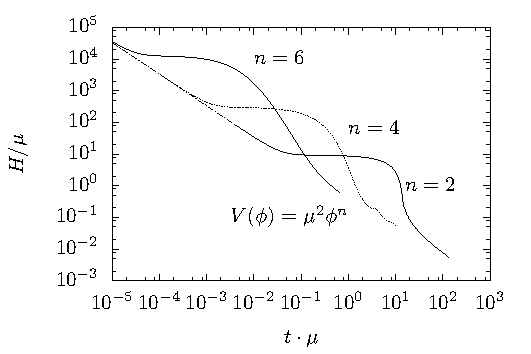
\includegraphics[width=\textwidth]{chapters/kinetic_dominance/figures/Hpol}
  \caption{The evolution of the Hubble parameter for three polynomial potentials of the form in~\eqref{eqn:polpot}. The axes have been rescaled in terms of the parameter \(\mu\) in the potential, so that this graph describes the evolution for any choice of \(\mu\). The initial conditions for inflation were set using the flat-universe kinetic conditions, and the parameter \(\phip\) was chosen so as to give \(55\) \(e\)-folds of inflation. All three universes emerge in a kinetically dominated phase with \(H=1/(3t)\), before entering a slow-roll inflationary phase with \(H\sim\mathrm{constant}\). The universe then exits inflation, after which small `wiggles' in \(H\) can be seen. These are due to the field \(\phi\) executing oscillations about the base of the potential.}\label{fig:figure_Hpol}
\end{figure}
%

%
\begin{figure}[tp]
  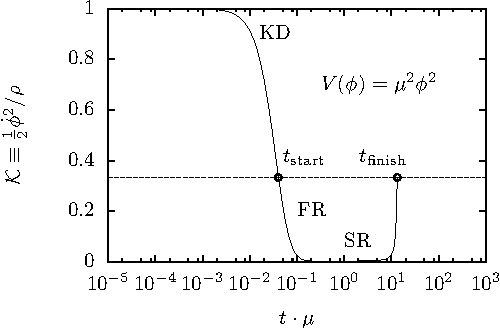
\includegraphics[width=\textwidth]{chapters/kinetic_dominance/figures/Kpol} 
  \caption{The evolution of \(\Kfrac = \frac{1}{2}\dot{\phi}^2/\rho\) for the quadratic inflaton potential \(V(\phi) = \mu^2 \phi^2\).  The universe can be seen to begin in a kinetically dominated state (KD).  It enters inflation at \(t_\mathrm{start}\). There is a brief fast-roll (FR) phase of inflation, before the universe enters a protracted slow-roll (SR) phase. The universe exits inflation at time \(t_\mathrm{finish}\) after \(55\) \(e\)-folds. After the end of inflation the field \(\phi\) executes oscillations about the base of the potential. This causes \(\Kfrac\) to oscillate rapidly between \(0\) and \(1\). For clarity, the value of \(\Kfrac(t)\) with \(t>t_\mathrm{finish}\) has not been plotted. The above behavior is common to all of the  polynomial potentials shown in Figure~\protect\ref{fig:figure_Hpol}.}\label{fig:figure_Kpol}
\end{figure}
%

The evolution of the Hubble parameter is shown in Figure~\ref{fig:figure_Hpol} for polynomials with \(n=2,4,6\). It is helpful to define the variable:
%
\begin{equation}
  \Kfrac 
  \equiv  
  \frac{\frac{1}{2}\dot{\phi}^2  }{\rho}  
  =  
  \frac{\frac{1}{2}\dot{\phi}^2  }
  {\frac{1}{2}\dot{\phi}^2 + V(\phi)},
\end{equation}
%
to be used as an investigative tool. \(\Kfrac\) is the ratio of the kinetic energy to the total energy and has the properties that:
%
\begin{equation}
  \Kfrac 
    \left\{
    %
    \begin{array}{rl}
      \approx 1 &\Rightarrow \hbox{kinetic dominance} 
      \\
      >\frac{1}{3} &\Rightarrow \hbox{not inflating}
      \\
      <\frac{1}{3} &\Rightarrow \hbox{fast-roll/power-law inflation}
      \\
      \approx 0 &\Rightarrow \hbox{slow-roll inflation.}
    \end{array}
%
    \right.
\end{equation}
%
This is used as a diagnostic tool in Figure~\ref{fig:figure_Kpol} for the quadratic potential \(V(\phi) = \mu^2\phi^2\). Examining Figure~\ref{fig:figure_Kpol} one can see that our earlier expectations are verified. There are four stages of evolution:
%
\begin{enumerate}
  \item the universe emerges from an initial singularity in a
    kinetically dominated phase,
  \item it transitions through fast-roll inflation,\label{itm:fr}
  \item before entering a protracted slow-roll phase, 
  \item and thereafter the field \(\phi\) quickly moves towards a minimum of the potential, about which it executes a decaying oscillation.
\end{enumerate}
%
The fast-roll transition in point~\eqref{itm:fr} is potentially responsible for the damping of the CMB spectrum at low-\(\ell\) observed in recent cosmological data. This will be discussed more fully in Section~\ref{sec:powspec}.


\subsection{Exponential potentials}
\label{sec:Exponential_potentials}
We now consider inflaton potentials of the form:
%
\begin{equation}
  \Vpow(\phi) 
  = 
  2V_0\left[
  \cosh\left(\frac{\sqrt{2\epsilon}}{\m}\phi\right)-1
  \right],
  \label{eqn:coshpot}
\end{equation}
%
which is a symmetrized form of the more common exponential potential; as \(\phi\rightarrow\pm\infty\) the potential takes the asymptotic form:
%
\begin{equation}
  V(\phi) 
  = 
  V_0 \exp\left(\frac{\sqrt{2\epsilon}}{\m} |\phi|\right).
  \label{eqn:exp_pot}
\end{equation}
%
Exponential potentials~\eqref{eqn:exp_pot} have been well studied \citep{yokoyama_dynamics_1988}. For potentials of this form, the evolution equations have the analytical power-law solutions:
%
\begin{align}
  a(t) 
  &\propto 
  {t}^{1/\epsilon},
  \label{eqn:pow_law_a_sol}
  \\
  \phi(t)
  &=
  \pm\m\sqrt{\frac{2}{\epsilon}}
  \log\left(\sqrt{\frac{V_0}{\left(3-\epsilon\right)}}
  \frac{\epsilon}{\m} t\right),
  \\
  H(t)
  &=
  \frac{1}{\epsilon t}.  
  \label{eqn:pow_law_H_sol}
\end{align}
%
It is worth noting that for mathematical consistency one requires \(\epsilon < 3\). For \(\epsilon<1\) these solutions are (continuously) inflating and are thus termed `power-law inflation' \citep{lucchin_power-law_1985}. Moreover, these are attractor solutions as the universe evolves forwards in time. It is also straightforward to show that at all epochs \(\dot{\phi}^2/V(\phi) = 2\epsilon/(3-\epsilon)\), so the ratio of the inflaton kinetic energy to its potential energy is constant. In particular, one notes that the solution is kinetically dominated only in the limit \(\epsilon \to 3\).  We may also interpret \(\epsilon\) as the slow-roll parameter:
%
\begin{equation}
  \epsilon\equiv\epsilon_H = -\frac{\dot{H}}{H^2},
\end{equation}
%
although one does not need to assume that it is small.

At first sight, solutions~\eqref{eqn:pow_law_a_sol}--\eqref{eqn:pow_law_H_sol} appear to represent a counterexample to kinetic dominance as \(t \to 0\), so it is worth exploring them further in the context of our proof of the generic nature of kinetic dominance in Section~\ref{sec:The_generic_nature_of_kinetic_dominance}. 

In terms of the master equation~\eqref{eqn:master_eq}, in a flat universe, one finds \(\phi = \sqrt{\frac{2}{3}}\m \psi + \mathrm{const} \) and thus for the exponential potential~\eqref{eqn:exp_pot}:
%
\begin{equation}
  \frac{\d{}}{\d{\psi}} \log \Vpow = \frac{2\epsilon}{\sqrt{3}}. 
\end{equation}
%
Consequently, the master equation has the constant, finite solution:
%
\begin{equation}
  f(\psi) = \log{\left(1-\frac{4}{3}\epsilon^2\right)}^{-1/2}.
  \label{eqn:uf_power_law}
\end{equation}
%
However, from the proof in Section~\ref{sec:The_generic_nature_of_kinetic_dominance}, we know that this finite solution is unique. Any solution which is greater than this diverges as \(|\phi|\to\infty\), and any solution less than this becomes negative.  Indeed, this is already evident from the fact that the power-law solutions are attractors as the universe evolves forwards in time. By the same token, these solutions are unstable in the limit \(t \to 0\), i.e.\ traveling backwards in time one diverges away from these solutions and generically arrives at kinetic dominance or a turn-around.  We note that the proof that the power-law solutions are attractors is due to~\cite{halliwell_scalar_1987}, and our work in Section~\ref{sec:The_generic_nature_of_kinetic_dominance} demonstrates that Halliwell's methodology is applicable more generally.

%
\begin{figure}[tp]
  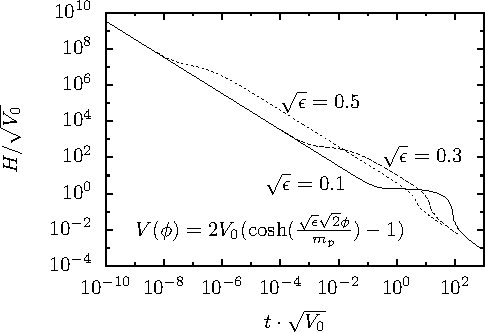
\includegraphics[width=\textwidth]{chapters/kinetic_dominance/figures/Hlam}
  \caption{As in Figure~\protect\ref{fig:figure_Hpol}, but for the hyperbolic cosine potential~\protect\eqref{eqn:coshpot}, which tends to an exponential potential for \(\phi \to \pm\infty\). The scaling constant is now \(\sqrt{V_0}\), and three values of \(\sqrt{\epsilon}\) are considered. One can see clearly that the universe emerges in a kinetically dominated state with \(H=1/(3t)\). The universe then enters a protracted power-law phase where \(H = 1/(\epsilon t)\). The field \(\phi\) oscillates about the base of the potential after the exit of the inflationary phase, causing wiggles in the later sections of the above plot.}\label{fig:figure_Hlam}
\end{figure}
%

%
\begin{figure}[tp]
  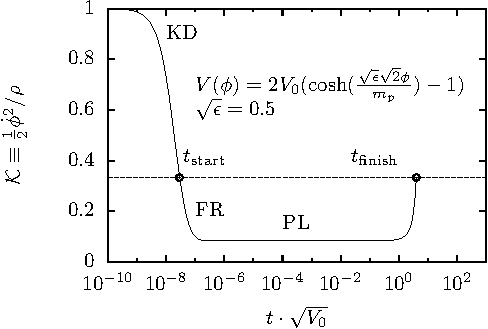
\includegraphics[width=\textwidth]{chapters/kinetic_dominance/figures/Klam}
  \caption{As in Figure~\protect\ref{fig:figure_Kpol}, but for the hyperbolic cosine inflaton potential with \(\sqrt{\epsilon}=0.5\). The universe emerges in a kinetically dominated (KD) phase before going through transitory fast-roll (FR). Instead of a slow-roll inflation, the universe then settles into a power-law inflation (PL), characterized by \(\Kfrac=\epsilon/3\). The universe exits inflation at \(t_\mathrm{finish}\), after which \(\phi\) executes oscillations about the base of the potential. \(\Kfrac\) therefore oscillates rapidly between \(0\) and \(1\), and the later \(t>t_\mathrm{finish}\) section of this plot has been suppressed for clarity.}\label{fig:figure_Klam}
\end{figure}
%

We show the evolution of the universe governed by the hyperbolic cosine inflaton potential~\eqref{eqn:coshpot} in Figures~\ref{fig:figure_Hlam}~\&~\ref{fig:figure_Klam}. The analysis is the same as that presented in Section~\ref{sec:section_polynomial_potentials}.  As in our previous example, the universe emerges from the initial singularity in kinetic dominance, which then transitions through a brief period of fast-roll inflation into a generically long-lasting power-law inflation state until the exit is reached as \(\phi\rightarrow0\), which corresponds to the minimum of the potential.  

\subsection{Another example of a finite solution \(f(\psi)\)}
%
\begin{figure}[tp]
  \centering
  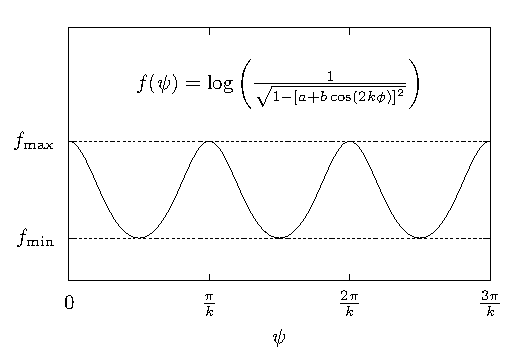
\includegraphics[width=\textwidth]{chapters/kinetic_dominance/figures/uf}
  \caption{An oscillating finite solution to the master equation~\protect\eqref{eqn:master_eq} with \(V(\psi)\) defined as in equation~\protect\eqref{eqn:Vphi_uf_example} and demonstrated in Figure~\protect\ref{fig:figure_ospot}. If \(a\) and \(b\) are chosen such that \(a>b>0\), \(0<a+b<1\), \(0<a-b<1\), then this represents a finite, positive solution.  From equation~\protect\eqref{eqn:uf_example} it is easy to see that \(\fmn = \log\left(\frac{1}{\sqrt{1-{(a+b)}^2}}\right)\), \(\fm=\log\left(\frac{1}{\sqrt{1-{(a-b)}^2}}\right)\).}\label{fig:figure_uf}
\end{figure}

%
\begin{figure}[tp]
  \centering
  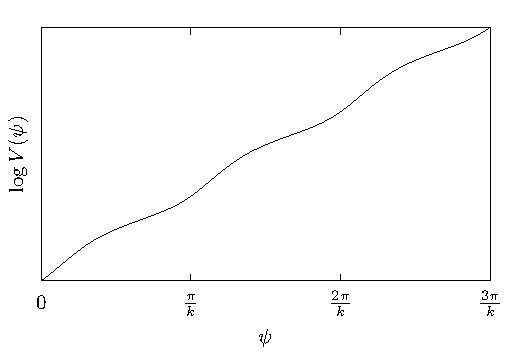
\includegraphics[width=\textwidth]{chapters/kinetic_dominance/figures/ospot}
  \caption{The master equation may be solved for the potential \(V(\psi)\) if a form of \(f(\psi)\) is chosen. For the choice of \(f(\phi)\) detailed in equation (\protect\ref{eqn:uf_example}), the potential is solvable in closed form [equation \protect\ref{eqn:Vphi_uf_example}].}\label{fig:figure_ospot}
\end{figure}
%

%
The \(f(\psi)\) described above in equation~\eqref{eqn:uf_power_law} is one of the simplest examples of a finite solution. As shown earlier, there is at most one such finite solution for any given potential. For concreteness we demonstrate another less trivial example in this section.

By reverse-engineering the master equation~\eqref{eqn:master_eq_f}, one can find a potential \(V(\psi)\) for any specified \(f(\psi)\). For example, if one chooses the oscillating solution (shown in Figure~\ref{fig:figure_uf}):
%
\begin{equation}
  f(\psi) = \log\left( \frac{1}{\sqrt{1-{[a+b\cos(2k\psi)]}^2}}\right),
  \label{eqn:uf_example}
\end{equation}
%
then this \(f(\psi)\) is the finite solution of the potential defined by:
%
\begin{equation}
	V(\psi)
    =
    \left[ 1-{(a+b \cos2k\psi)}^2 \right]
    e^{2 a \psi +\frac{b}{k} \sin 2k\psi},
    \label{eqn:Vphi_uf_example}
\end{equation}
whose shape is detailed in Figure~\ref{fig:figure_ospot}.
%

To show explicitly that this is the only finite solution in this case, we consider a perturbed solution \(y(\psi) = f(\psi)+\delta(\psi)\).  From the uniqueness theorem (Section~\ref{sec:uniqueness_theorem}) if \(\delta\) is initially positive (negative), then it is positive (negative) for all \(\psi\). From the master equation~\eqref{eqn:master_eq} one may show that the perturbed solution satisfies:
%
\begin{align}
  \frac{\d{}}{\d{\phi}}\delta 
  =& 
  \sqrt{1-e^{-2(f+\delta)}} -\sqrt{1-e^{-2f}}, 
  \label{eqn:perturb}
  \\
  &>
  \sqrt{1-e^{-2(\fm+\delta)}} -\sqrt{1-e^{-2\fm}}
\end{align}
%
where \(\fm = \log(1/\sqrt{1-{(a-b)}^2})\). Substituting this in, one finds:
%
\begin{align}
  \frac{\d{}}{\d{\phi}}\delta 
  > 
  \sqrt{1-e^{-\delta}({1-{(a-b)}^2})} - \sqrt{1-({1-{(a-b)}^2})}
\end{align}
%
One can see that if \(\delta>0\), then the right-hand side is strictly greater than some number greater than zero, hence \(\delta\) grows without bound, and any solution greater than \(f\) initially diverges. 

Working from equation~\eqref{eqn:perturb}, one also finds:
%
\begin{align}
  \frac{\d{}}{\d{\phi}}\delta 
  <&
  \sqrt{1-e^{-2(\fmn+\delta)}} -\sqrt{1-e^{-2\fmn}} 
  \nonumber
  \\
  &<
  \sqrt{1-e^{-\delta}({1-{(a+b)}^2})} - \sqrt{1-({1-{(a+b)}^2})}
\end{align}
%
One can see that if \(\delta<0\), then the right-hand side is strictly less than some number less than zero, hence \(\delta\) falls without bound, and any solution less than \(f\) eventually becomes negative. 

Thus one finds that \(f(\psi)\) is the only finite positive solution.  All other solutions either become negative or diverge.




\subsection{Power spectrum of the curvature perturbation}
\label{sec:powspec}
%
\begin{figure}[tp]
  \centering
  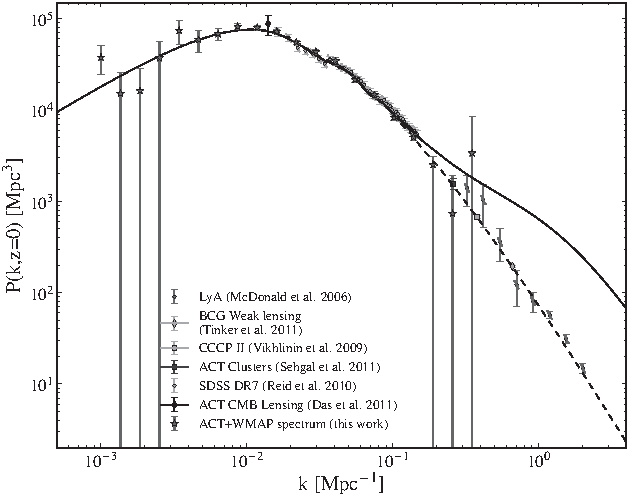
\includegraphics[width=\textwidth]{chapters/kinetic_dominance/figures/powerspec}
  \caption{Figure taken from~\protect\cite{hlozek_atacama_2012} showing the current status of the observed late-time matter perturbation power spectrum. As one can see, the currently probed \(k\) range is \(10^{-3}<k<2\:\mathrm{Mpc}^{-1}\).}\label{fig:experimental_power_spectrum}
\end{figure}
%

The most interesting aspect of kinetic dominance is seen when the power spectrum of scalar curvature perturbations is examined. Recent observations of CMB power spectra \citep{hinshaw_nine-year_2012,planck_collaboration_planck_2013} show an unexpected suppression at low multipoles. While these deviations are not large enough to cause us to discard the standard \(\Lambda\) cold dark matter (\(\Lambda\)CDM) cosmology \citep{1998PhRvD..57.2207B,2000PhRvD..62l3513B,2004PhRvD..69f3516D}, there is still enough tension to be worthy of investigation.  As we show below, kinetic dominance predicts a generic cutoff in the curvature power spectrum at large spatial scales. This is precisely what is needed to suppress low multipole moments of the CMB power spectrum while retaining the quality of the fit at higher \(\ell\) values.

Figure~\ref{fig:experimental_power_spectrum} has been taken from~\cite{hlozek_atacama_2012} and shows the current status of the observational constraints on the late-time matter power spectrum, given by:
%
\begin{equation}
  P(k,z=0) = 2\pi^2 k \mathcal{P}_\mathcal{R}(k) G^2(z) T^2(k),
\end{equation}
%
where \(G(z)\) gives the growth of matter perturbations, \(T(k)\) is the matter transfer function and \(\mathcal{P}_\mathcal{R}(k)\) is the primordial curvature perturbation power spectrum. This mapping enables one to combine constraints on the power spectrum from CMB and other probes at \(z\approx 0\).




As shown by~\cite{liddle_cosmological_2000}, the primordial curvature perturbation power spectrum \(\mathcal{P}_{\mathcal{R}}(k)\) is given approximately by:
%
\begin{equation}
  \mathcal{P}_{\mathcal{R}}(k)
  =
  {\left(\frac{H^2}{2\pi\dot{\phi}}\right)}^2_{k=a H},
  \label{eqn:curvature_power_spectrum}
\end{equation}
%
where, as denoted, the right-hand side is evaluated when a given scale crosses the horizon. If one has numerically calculated \(a(t)\), \(H(t)\) and \(\dot{\phi}(t)\), then plotting \({\left(H^2/ 2\pi\dot{\phi}\right)}^2\) against \(aH\) will give the shape of the spectrum.

In order to perform predictive calculations, one must calibrate the \(aH\) axis to an observable scale today. This is easy to do if one defines a comoving pivot scale \(k_*\), which leaves the horizon (at a time \(t_*\)) when \(N_*\) \(e\)-folds of inflation remain. In general, the relation between \(k_*\) and \(N_*\) depends on both the potential \(V(\phi)\) and the details of cosmic reheating. For most reasonable models, \(50<N_*<60\)  for \(k_*\) with a value of \(0.05\:\mathrm{Mpc}^{-1}\) today \citep{planck_collaboration_planck_2013-1}. For this work, we will take \(N_*=55\). 

Once a value for \(N_*\) is chosen, one can determine numerically the time \(t_*\) at which \(N_*\) \(e\)-folds of inflation remain as well as \(a_*\equiv a(t_*)\) and \(H_*\equiv H(t_*)\). Since we know that the value of \(aH\) at \(t_*\) corresponds to a wave number today of \(0.05\:\mathrm{Mpc}^{-1}\), we may calibrate the \(aH\) axis of the plot of the power spectrum using:
%
\begin{equation}
  k_\mathrm{today} 
  = 
  \frac{aH}{a_*H_*}\times0.05\:\mathrm{Mpc}^{-1}.
\end{equation}
%
Calibrated plots of \(\mathcal{P}_\mathcal{R}(k)\) are found in Figures~\ref{fig:figure_CSpol} and \nolinebreak\ref{fig:figure_CSlam}. 


%
\begin{figure}[tp]
  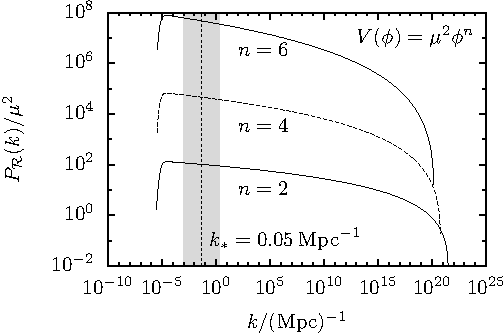
\includegraphics[width=\textwidth]{chapters/kinetic_dominance/figures/CSpol}
  \caption{The approximate power spectrum of the primordial curvature perturbations for polynomial potentials, calculated using equation~\protect\eqref{eqn:curvature_power_spectrum}. The units of the \(k\) axis are determined by the requirement that there are \(N_*=55\) \(e\)-folds remaining when the pivot scale \(k_*=0.05\:\mathrm{Mpc}^{-1}\) exits the horizon \(k=aH\). The magnitude of the power spectrum is determined by the scaling \(\mu\) in the potential. The grey area indicates the angular scales that have been experimentally probed; see Figure~\protect\ref{fig:experimental_power_spectrum}.}\label{fig:figure_CSpol}
\end{figure}
%

%
\begin{figure}[tp]
  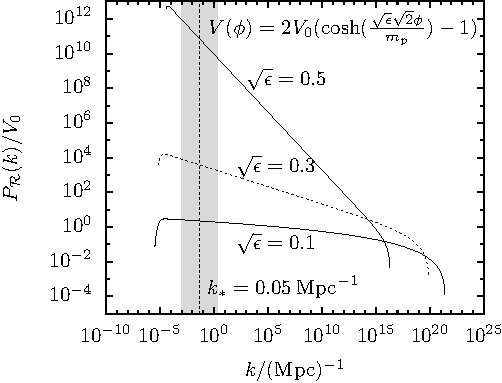
\includegraphics[width=\textwidth]{chapters/kinetic_dominance/figures/CSlam}
  \caption{As in Figure~\protect\ref{fig:figure_CSpol}, but for exponential potentials. The magnitude of the power spectrum now scales with \(V_0\) rather than \(\mu^2\).}\label{fig:figure_CSlam}
\end{figure}
%



The shape of the primordial power spectra obtained corresponds to that found in~\cite{lasenby_closed_2003}. We see that, in general, \(\mathcal{P}_\mathcal{R}(k)\) has less power at low and high \(k\) values than would be expected from a canonical power-law primordial spectrum.  The low-\(k\) cutoff is entirely generic and occurs as a result of the brief period of fast-roll prior to slow-roll or power-law inflation.  This effect has been discussed previously by~\cite{boyanovsky_cmb_2006}. The fast-roll regime behaves like an attractor potential in the wave equations for the mode functions of curvature and tensor perturbations. This potential leads then to the suppression of the primordial power spectra at low \(k\).  Hence, it might be able to account for the suppression of the quadrupole of the CMB in agreement with observational data, as discussed by~\cite{boyanovsky_cmb_2006-1}.  The exact position of the low-\(k\) cutoff is determined by the value of \(\phip\), as it controls the total number of \(e\)-folds of inflation. This effect has also been discussed in the context of ``Open Inflation'' \citep{Yamauchi_strings_2011,Linde_open_1999,Linde_toy_1999}, and examined using WMAP data by~\cite{Contaldi_suppress_2003}.

Further inspection shows \(\mathcal{P}_\mathcal{R} \sim \log k\) after the low-\(k\) cutoff. This is identical to the result found by~\cite{lasenby_closed_2003} and in contrast with the standard power-spectrum parametrization which assumes a near-flat power-law scaling: \(\log\mathcal{P}_\mathcal{R}\sim \log k\). 

 
It should be observed that we are using the approximation~\eqref{eqn:curvature_power_spectrum} outside the slow-roll regime for which it is valid; nonetheless we have performed full calculations that do not use the above approximation and which indicate that the resulting power spectrum is, in fact, a good representation of the true spectrum. These approximate spectra demonstrate the key generic aspects of the accurate calculation: both exhibit a low-\(k\) cut off and that \(\mathcal{P}_\mathcal{R}(k) \sim \log(k)\).  We shall follow this work with a second publication containing the full details and discussion of the accurate calculation. An alternative but related accurate calculation has been performed by~\cite{Lello_tensor_2013}, which uses kinetic initial conditions to show that the suppression at low-\(\ell\) is entirely generic. It should also be noted that methods which reconstruct the primordial power spectrum \(\mathcal{P}_\mathcal{R}(k)\) \citep{vazquez_reconstruction,Hazra_reconstruction_2013} using data also show a dip at low \(k\) values.

%
\begin{figure}[tp]
  \centerline{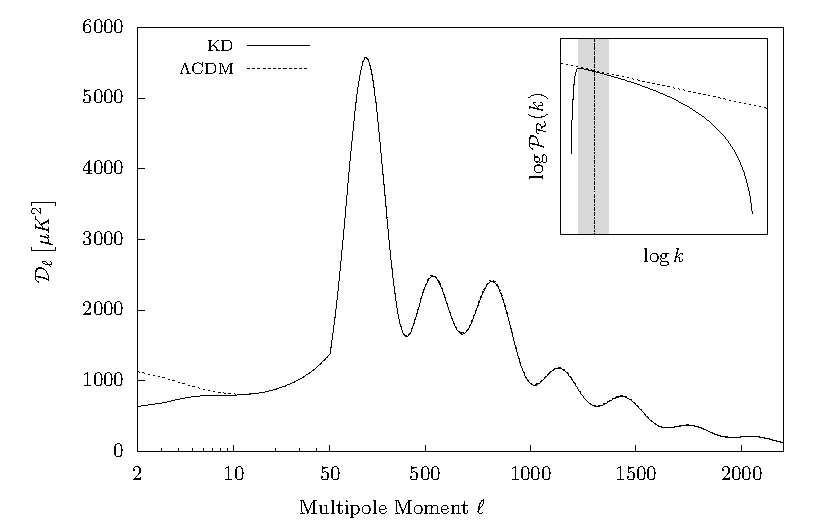
\includegraphics[width=\textwidth]{chapters/kinetic_dominance/figures/Cl}}
  \centerline{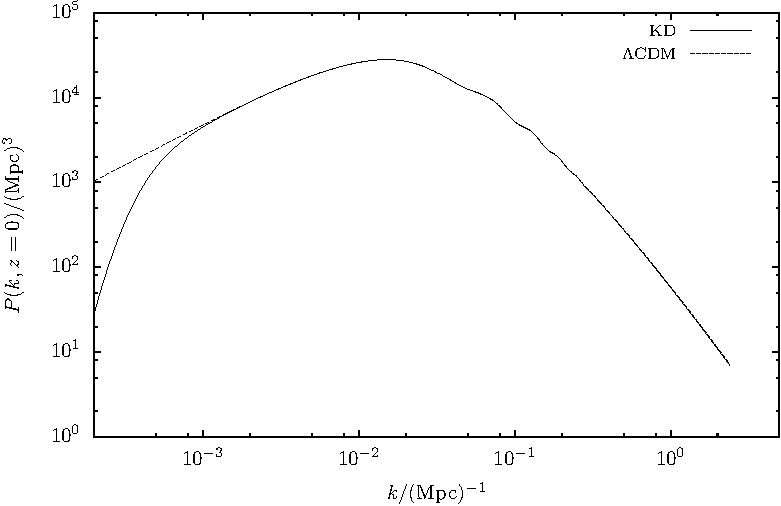
\includegraphics[width=\textwidth]{chapters/kinetic_dominance/figures/matter}}
  \caption{The CMB scalar power spectra (top) and the late-time matter power spectra (bottom), resulting from the curvature perturbation power spectra in the inset of the top figure. The solid line corresponds to a free inflaton with potential \(V=\frac{1}{2}m^2\phi^2\) assuming kinetic initial conditions with \(m=0.81\times10^{-5}\m\), \(\phip = 21.8\), \(N_*=42.5\). The dashed line corresponds to the best-fit standard \(\Lambda\)CDM model.  The presence of the cutoff in the curvature power spectrum for kinetic initial conditions causes a suppression of power on large angular scales in both the CMB and matter power spectra.}\label{fig:figure_Cl}
\end{figure}
%

We demonstrate the suppression on large angular scales of the CMB and late-time matter power spectra qualitatively in Figure~\ref{fig:figure_Cl}.  In the standard six-parameter \(\Lambda\)CDM cosmology, the primordial power spectrum has a power-law form, parametrized by two variables \(A_s\) and \(n_\mathrm{s}\), such that:
%
\begin{equation}
  P_\mathcal{R}(k) = A_s{\left(\frac{k}{k_*}\right)}^{n_\mathrm{s}-1}
\end{equation}
%
Using the best-fit parameters from {\em Planck\/}+WP+highL+BAO \citep{planck_collaboration_planck_2013} yields the standard matter CMB power spectra (dashed lines), whereas the alternative power spectra (solid line) were generated using \(\mathcal{P}_\mathcal{R}(k)\) from Figure~\ref{fig:figure_CSpol} (for \(n=2\)), for which the axes were rescaled to agree with the values of \(A_s\) and \(n_\mathrm{s}\) during the slow-roll phase. The resulting matter and CMB power spectra are seen to exhibit a suppression of power at low \(k\) and \(\ell\) values, with the rest of the spectra perfectly intact, as required by cosmological observations.  Further investigation is clearly required, but this analysis already demonstrates the utility of kinetic dominance.

The results of this section agree with the ``just enough inflation'' scenario introduced by~\cite{Ramirez_excluded_2009,Ramirez_predictions_2012,Ramirez_low_2012}.  In their work they assume that there is some physical mechanism which would limit the potential from above such that \(V(\phi)<M_\mathrm{GUT}^4\), and thus find that \(V(\phi)\ll\dot{\phi}^2\) at early times. Our results therefore place their observations in a more generic setting.


\subsection{Comparison with equipartition initial conditions}
\label{sec:comparison}

An alternative method for setting the initial conditions for inflation models has been proposed by~\cite{boyanovsky_cmb_2006}. Their work also shows that the low-multipole suppression of the scalar power spectrum is the result of a brief period of fast-roll inflation prior to the standard slow-roll regime. They arrange for such a fast-roll period by assuming ``equipartition initial conditions''. In this approach, the initial conditions are set at a time \(t=\teq\), when there is approximate equipartition between the kinetic and potential energy of the inflaton:
%
\begin{equation}
  \frac{1}{2}\phideq \sim V(\phieq).
  \label{eqn:bvsbc}
\end{equation}
%
Almost by definition, the subsequent evolution will generically exhibit a (brief) period of fast-roll inflation, before entering a slow-roll phase (which is an attractor solution). BVS verified this generic behavior for a wide range of chaotic and new inflation potentials.

To address these issues further, we consider in more detail the main inflationary model used by BVS to illustrate their generic findings.  The model is spatially flat, and uses a ``new inflation'' potential:
%
\begin{equation}
  V(\phi) =V_0{\left(1-\mu\phi^2\right)}^2.
\end{equation}
%
The initial conditions are set by choosing \(\phi(\teq)=\phieq=0\) with an equipartition of kinetic and potential energies so that \(\dot{\phi}(\teq)=\phideq=\sqrt{2V_0}\).  Figure~\ref{fig:figure_BVS_initial_conditions} illustrates this diagrammatically.  The values of \(V_0\) and \(\mu\) are tuned so that the power spectrum has an appropriate index \(n_s\) and the correct number of \(e\)-folds are generated.

%
\begin{figure}[tp]
  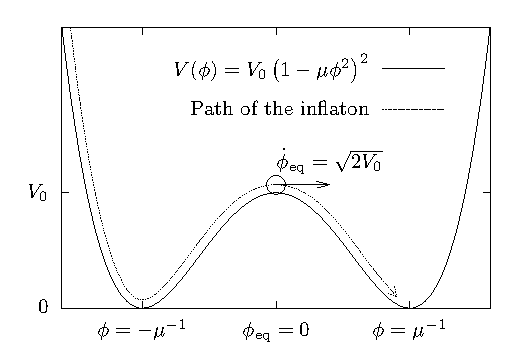
\includegraphics[width=\textwidth]{chapters/kinetic_dominance/figures/newpot}
  \caption{An illustration of the ``equipartition'' initial conditions imposed by~\protect\cite{boyanovsky_cmb_2006}, for the new inflation potential \(V_0{\left(1-\mu^2\phi^2\right)}^2\). The initial conditions are set at some time \(\teq\) with values denoted by a subscript ``eq''. The field is set with \(\phieq=0\) and a velocity \(\phideq= \sqrt{2V_0}\) so that the energy is partitioned equally between kinetic and potential energy: \(V(\phieq) = \frac{1}{2}\phideq\).}\label{fig:figure_BVS_initial_conditions}
\end{figure}
%

We now interpret this methodology using our formalism. Kinetic initial conditions will inevitably lead to a time \(\teq\) when the equipartition condition~\eqref{eqn:bvsbc} is satisfied. Thus, rather than considering~\eqref{eqn:bvsbc} as a fundamental physical principle, it should be regarded as a natural consequence of kinetic initial conditions. Moreover, this is true independently of any tuning that we apply to \(\mu\) or \(V_0\) and indeed of the potential. Moreover, demanding that~\eqref{eqn:bvsbc} is satisfied at \(\phi=0\) corresponds to choosing a specific value of \(\phip\) such that the field arrives at \(\phi=0\) with an equipartition of kinetic and potential energy (This is illustrated in Figure~\ref{fig:figure_BVS_initial_conditions}).  If, however, \(\phip\) is required to lie within a certain range of values in order to produce an appropriate number of \(e\)-folds of inflation, then the choice \(\phieq=0\) may be inconsistent with kinetic dominance. This can only be resolved if one is free to choose a general point \(\phieq\) for the position of equipartition.  

\section{When is kinetic dominance not the case?}
\label{sec:When_is_kinetic_dominance_not_the_case?}
Having looked in detail at the consequences of kinetic dominance, we enumerate the instances in which it does not hold. If kinetic dominance is not the case, then we can conclude that either
%
\begin{enumerate}
    \item as one moves backward in time \(\dot{\phi}\to 0\), and the inflaton tends to a constant value; or
    \item there is no epoch before which we can say \(\dot{\phi}\ne 0\), and the inflaton continues to oscillate as one moves backward in time.
\end{enumerate}
%
We shall examine each of these cases in turn.

\subsection{Resting inflaton: \(\dot{\phi}\to 0\)}


\subsubsection{No auxiliary fluids: eternal de Sitter}
We shall begin by considering the case with no auxiliary fluids, for which the Friedmann~\eqref{eqn:Friedmann_mod} and Klein-Gordon~\eqref{eqn:Klein_Gordon_mod} equations take the form:
%
\begin{align}
  H^2 
  &=
  \frac{1}{3\m^2}\left(\tfrac{1}{2}\dot{\phi}^2 + V(\phi) \right)
  \label{eqn:Friedmann_dotphi_to_zero_no_fluid} 
  \\
  0
  &=
  \ddot{\phi} +3\dot{\phi}H + V^\prime(\phi).
  \label{eqn:Klein_Gordon_dotphi_to_zero_no_fluid}
\end{align}
%
If \(\dot{\phi}\to 0\) as one moves backward in time, then the inflaton \(\phi\) and field \(V(\phi)\) tend to constant values \(\phiz\) and \(V(\phiz)\equiv V_0\). By examining the first of the above equations, one can see that \(H\) tends to a constant value:
%
\begin{equation}
  H\to H_0 \equiv \sqrt{\frac{V_0}{3\m^2}}.
\end{equation}
%
Thus, such a universe exhibits an eternal de Sitter phase (edS) as \(t\to-\infty\).

By examining the Klein-Gordon equation~\eqref{eqn:Klein_Gordon_dotphi_to_zero_no_fluid}, one can see that the only nonzero term remaining is \(\frac{\d{}}{\d{\phi}}V(\phi)\). From this one can conclude that the inflaton must come to rest on an extremum of the potential. It is straightforward to show that the dynamical equations then have the following asymptotic solution as \(t \to -\infty\):
%
\begin{align}
  \phi(t)
  &=
  \phiz \pm A \exp(\alpha t),\\
  H(t)
  &=
  \sqrt{\frac{V(\phiz)}{3\m^2}} \equiv H_0,\\
  a(t)
  &=
  B e^{H_0t},
\end{align}
%
where \(A\) and \(B\)  are arbitrary constants, and \(\alpha\) is a real, positive solution to the quadratic equation:
% 
%
\begin{equation}
  \alpha^2 + 3H_0\alpha + \left.
  \frac{{d^2}V}{{d}\phi^2}\right|_{\phi=\phiz}=0.
\end{equation}
%
This solution is discussed in more detail by~\cite{destri_preinflationary_2010}. An example of this is ``Hilltop inflation'' \citep{linde_1982,albrecht_1982}. 

It should be noted that these solutions are not generic, as these solutions are rolling away from a position of unstable equilibrium: going backward in time, any small perturbation causes the inflaton to overshoot the extremum and move on to a kinetically dominated phase.

One can demonstrate the above statement formally by considering equations~\eqref{eqn:Klein_Gordon_dotphi_to_zero_no_fluid} and~\eqref{eqn:Friedmann_dotphi_to_zero_no_fluid} in the Hamilton-Jacobi representation:
%
\begin{align}
  {\left(\frac{\d{H}}{\d{\phi}}\right)}^2
  &=
  \frac{3H^2}{2\m^2} - \frac{V(\phi)}{2\m^4}
  \\
  \frac{\d{H}}{\d{\phi}}
  &=
  -\frac{\dot{\phi}}{2\m^2}.
\end{align}
%
The Hamilton-Jacobi representation is valid in the periods in which \(\phi(t)\) is monotonic; i.e. \(\dot{\phi}\) does not change sign. If one assumes that \(\dot{\phi}>0\), then the first of the above equations reads:
%
\begin{equation}
  \frac{\d{H}}{\d{\phi}} 
  = 
  -\sqrt{\frac{3H^2}{2\m^2} - \frac{V(\phi)}{2\m^4}}.
  \label{eqn:Hamilton_Jacobi_H}
\end{equation}
%
Solutions to this equation are plotted in Figure~\ref{fig:figure_edS}, which demonstrates the following facts: 
%
\begin{itemize}
  \item There is a region in which solutions cannot exist, since by the Friedmann equation~\eqref{eqn:Friedmann_dotphi_to_zero_no_fluid} we find that \(H>\sqrt{V(\phi)/3\m^2}\).
  \item  By equation~\eqref{eqn:Hamilton_Jacobi_H} that solutions meet this region with zero gradient.
  \item Outside of this region, the right-hand side of equation~\eqref{eqn:Hamilton_Jacobi_H} is Lipschitz continuous~\citep[see Section~\ref{sec:uniqueness_theorem}, or][]{agarwal_1993}, hence solutions do not cross over in the white region of the graph.
\end{itemize}
% 

Consider the eternal de Sitter solution \(\HedS(\phi)\), plotted as the right-hand half of the dotted line in Figure~\ref{fig:figure_edS}.  This solution has the property that as \(\phi\to\phiz\), \(\dot{\phi}\propto\frac{\d{H}}{\d{\phi}}\to0\). Consider also a solution \(\Hh\) which at some value \(\phi_1\) is greater than the edS solution, \(\Hh(\phi_1) \ge \HedS(\phi_1)\). By uniqueness, this will remain greater than \(\HedS\) within the white region of the graph. Both \(\HedS\) and \(\Hh\) satisfy equation~\eqref{eqn:Hamilton_Jacobi_H}.  Taking the difference of these two equations and integrating from \(\phi_1\) to \(\phiz\) shows:
%
\begin{align}
  &\Hh(\phiz)-\HedS(\phiz)= \nonumber\\
  &\Hh(\phi_1)-\HedS(\phi_1) \nonumber\\
  & + \int_{\phiz}^{\phi_1} 
  \sqrt{\frac{3\Hh^2}{2\m^2} - 
  \frac{V(\phi)}{2\m^4}}-\sqrt{\frac{3\HedS^2}{2\m^2} - 
  \frac{V(\phi)}{2\m^4}}\:d\phi \nonumber \\
  &>\Hh(\phi_1)-\HedS(\phi_1)>0 \nonumber
\end{align}
%
We thus find \({\d{\Hh}}/{\d{\phi}}\ne0\) at \(\phi=\phiz\), and thus does not represent an eternal de Sitter phase. A similar argument holds for solutions \(\Hl(\phi)\) which start out less than \(\HedS\), only these must collide with the dark region. Upon this collision, \(\dot{\phi}\) changes sign, causing the diagram to reflect about the \(\phi=0\) axis.

Figure~\ref{fig:figure_edS} reveals an interesting second eternal de Sitter solution. The right-hand half of the dashed line indicates the previously discussed phase: a universe which emerges at \(t=-\infty\) in an inflating state with the inflaton slowly rolling off an extremum in the potential, exiting the inflationary phase when the inflaton oscillates about the bottom of the potential.  The left-hand half of the dashed line indicates a universe which emerges at \(t=0\) in a kinetically dominated phase before the inflaton rests on top of the extremum, settling into an eternal de Sitter phase as \(t\to\infty\).

%
\begin{figure}[tp]
  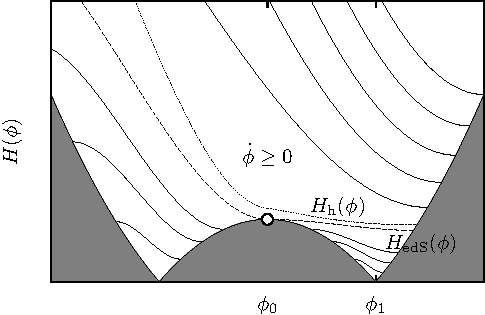
\includegraphics[width=\textwidth]{chapters/kinetic_dominance/figures/edS}
  \caption{Schematic of the Hubble parameter against \(\phi\) in the Hamilton-Jacobi representation. The potential \(V(\phi)\) is the same potential as in Figure~\protect\ref{fig:figure_BVS_initial_conditions}. The solid curves represent the portions of the solutions to~\protect\eqref{eqn:Hamilton_Jacobi_H} with \(\dot{\phi}\ge0\). The shaded region is defined by \(H<\sqrt{V/3\m^2}\). Solutions meet the shaded region with zero gradient. Solutions within the white region are unique: they do not cross over. The right-hand side of the dashed curve represents a universe entering at  \(\phi=\phiz\), (\(t=-\infty\)) in an eternal de Sitter phase. The left-hand side of the dashed curve indicates a universe entering in a kinetically dominated phase before settling into a de Sitter phase at \(t=+\infty\).}\label{fig:figure_edS}
\end{figure}
%

\subsubsection{Auxiliary fluids}
The presence of an auxiliary fluid makes it slightly easier to engineer a solution in which \(\dot\phi\to0\), as one does not require that the inflaton comes to rest on an extremum of the potential.

In the limit that \(a\to 0\), the \(\rho_i\) with the largest \(w_i\) dominates over all of the others. The relevant equations are therefore the Friedmann~\eqref{eqn:Friedmann_mod} and Klein-Gordon~\eqref{eqn:Klein_Gordon_mod} equations, with a single fluid \(\rho_w\):
%
\begin{align}
  H^2
  &=
  \frac{1}{3\m^2}\left(\tfrac{1}{2}\dot{\phi}^2
  + V(\phi)
  + \rho_w \right),
  \label{eqn:Friedmann_dotphi_to_zero} \\
  0
  &=
  \ddot{\phi} +3\dot{\phi}H + V^\prime(\phi).
  \label{eqn:Klein_Gordon_dotphi_to_zero}
\end{align}
%
In the first of these, if \(\phi\to\phiz\), then as \(a\to0\) on the right-hand side one only need worry about \(\rho_w\). Since \(H=\frac{\d{}}{\d{t}}\log a\), and \(\rho_w\propto a^{-3(1+w)}\), one finds:
%
\begin{align}
  \int\frac{\d{\log a}}{\sqrt{\rho_w}}
  &=
  \int\frac{t}{\sqrt3\m}
  \\
  \Rightarrow \qquad \rho_w
  &=
  \frac{4\m^2}{3{(1+w)}^2} \frac{1}{t^2}.
  \label{eqn:rho_dotphi_to_zero}
\end{align}
%
We may then use the above equation along with~\eqref{eqn:Friedmann_dotphi_to_zero} to show that:
%
\begin{equation}
  H = \frac{2}{3(1+w) t}
  \quad
  \Rightarrow \quad a\propto t^{2/3(1+w)}.
  \label{eqn:H_dotphi_to_zero}
\end{equation}
%
We can now solve~\eqref{eqn:Klein_Gordon_dotphi_to_zero} for \(\phi(t)\).  As \(\phi\to\phiz\), we may assume the potential term tends to a constant value \(\prm{V_0}\). Selecting the solution which tends to a constant, one finds:
%
\begin{equation}
  \phi(t) = \phiz -\frac{\prm{V_0}(w+1)}{2(w+3)}t^2.
\end{equation}
%
This constitutes a solution which is present for any potential with auxiliary fluids. In general one can find a specific solution with \(\phi\to\phiz\) for any given \(\phiz\). However, for any small perturbation from this solution, one arrives back at kinetic dominance. The kinetically dominated solutions are generic. 












\subsection{Pathological oscillations: \(\dot{\phi}=0\)}
\label{sec:pathological_oscillations}
We now turn to the case where there is no epoch prior to which \(\phi\) is monotonic. The inflaton continues to oscillate endlessly as \(a\to0\). 

It is easy to engineer potentials that lead to this behavior. In the case with no auxiliary fields, the limiting forms of \(\dot{\phi}(t)\) and \(\phi(t)\) are given by equations~\eqref{eqn:dotphi_of_t_flat} and~\eqref{eqn:phi_of_t_flat}. We may solve these to find the relationship between \(\dot{\phi}\) and \(\phi\):
%
\begin{equation}
  \dot{\phi}^2 = \exp\left(\frac{\sqrt{6}}{\m} |\phi-\phip|\right).
\end{equation}
%
If one chooses a potential that grows faster than the right-hand side of this equation, then the universe cannot be kinetically dominated.  We are thus forced to the conclusion that in such a universe either \(\dot{\phi}\to 0\) or there is no epoch before which \(\dot{\phi}\ne 0\).  Typically, if one examines the numerical solutions of such equations, one sees that the inflaton oscillates at a faster and faster rate, with greater and greater amplitude until the numerical limit of the solver is reached.

These solutions are therefore somewhat pathological, though for the cases where they occur, kinetic dominance is not the generic solution.









\section{Conclusions}
\label{sec:Conclusions}

We have shown that, if quantum gravitational effects are ignored, the coupled evolution equations for the inflaton field \(\phi(t)\) and the Hubble parameter \(H(t)\) in generic homogeneous and isotropic single-field inflation models imply that a universe beginning with a steadily moving inflaton (\(|\dot{\phi}| > \vellim > 0\) as \(a\to 0\), for some positive constant \(\vellim\)) generically emerges from an initial singularity in a noninflating, kinetically dominated state (\(\dot{\phi}^2 \gg V(\phi)\)).  In this kinetic-dominated regime, one obtains simple analytical solutions for \(\phi(t)\) and \(H(t)\), which are independent of the form of the inflaton potential \(V(\phi)\) and of the presence of auxiliary fluids such as matter, radiation, dark energy or spatial curvature. These solutions provide a simple means of setting the initial conditions for such inflation models, from which numerical integration of the evolution equations may proceed.

For illustration, we applied this ``kinetic'' procedure for setting initial conditions to a spatially flat polynomial and exponential inflation models.  By making an appropriate choice of the time \(\ti\) at which the initial conditions are set, and the single free parameter \(\phip\) in the analytic kinetic-dominated solution, all models produce an amount of inflation compatible with observations.  The background evolution in each case displays a generic behavior.  Following a noninflating period of kinetic dominance, \(H(t)\), \(\phi(t)\) and their time derivatives continue to decrease until one obtains approximate equipartition \(\dot{\phi}^2 \sim V(\phi)\) between the kinetic and potential energies of the inflaton. This marks the onset of a (typically brief) period of fast-roll inflation, which turns into a slow-roll [\(\dot{\phi}^2 \ll V(\phi)\)] or power-law inflation phase.  At the end of the slow-roll phase, the inflation quickly moves towards a minimum of the potential, about which it executes a decaying oscillation.

We calculated the approximate spectrum of scalar perturbations for the polynomial and exponential models and find, in both cases, that it contains less power at low- and high-\(k\) values than would be expected from a power-law behaviour. The low-\(k\) effect is a generic consequence of the kinetic initial conditions, for any consistent inflaton potential or spatial curvature, resulting in particular from the brief period of fast-roll inflation that they imply.  The damping of power on large scales may provide an explanation for the low-\(\ell\) falloff in the matter and CMB power spectra seen in recent cosmological observations.

We also compared our kinetic initial conditions with an alternative proposal by~\cite{boyanovsky_cmb_2006} that inflationary initial conditions should be set by assuming approximate equipartition between the kinetic and potential energy of the inflaton.  In the context of kinetic initial conditions, approximate equipartition is not a fundamental physical principle, but merely an inevitable consequence.  Moreover, by considering a particular model used by BVS, we demonstrate that assigning equipartition initial conditions with an arbitrary initial value for the inflaton field can lead to inconsistency with kinetic initial conditions.

Finally we enumerated the universes which do not have a steadily moving inflaton, and have shown that these are special cases, distinct from the generic kinetically dominated case.





\begin{subappendices}
  \section{Uniqueness theorem}
\label{sec:uniqueness_theorem}
We shall now prove that the solutions to the initial value problem of the master equation~\eqref{eqn:master_eq}:
%
\begin{align}
  \frac{\d{y}}{\d{\psi}}
  &=
  \sqrt{1-e^{-2y}} - \frac{\d{}}{\d{\psi}}\log \sqrt V,
  \label{eqn:IVP1}
  \\
  y(\psiz)
  &=
  y_0>0
  \label{eqn:IVP2},
\end{align}
%
are unique within any finite interval \(\psi\in[\psiz,\psi_1]\); i.e, if two positive solutions intersect at a point, then they intersect
everywhere.

We begin by putting a lower bound on \(y\) in the interval \([\psiz,\psi_1]\): From assumption~\eqref{eqn:conditions}, we know \(\dot{\phi}^2>\vellim^2>0\). If we unpack the definition of \(y\) using equations~\eqref{eqn:y_def},~\eqref{eqn:Ntrans},~\eqref{eqn:tau_def} and~\eqref{eqn:Friedmann_c}, one finds:
%
\begin{equation}
  y 
  = 
  \frac{1}{2}\log
  \left(\frac{\frac{1}{2}\dot{\phi}^2 + V(\phi)}{V(\phi)}\right) 
  > 
  \frac{\vellim^2}{4\Vm},
\end{equation}
%
where \(\Vm\) is the maximal value of \(V(\psi)\) in the interval \([\psiz,\psi_1]\). With this in hand we may prove the uniqueness of solutions of the initial value problem~\eqref{eqn:IVP1},~\eqref{eqn:IVP2} using standard techniques. For a good reference of such techniques the reader should consult the text by \citet{agarwal_1993}. In this case, we shall prove it using {\em Peano iteration}.


If one assumes that \(y(\psi)\) and \(z(\psi)\) are two distinct solutions, then their difference satisfies:
%
\begin{equation}
  \frac{\d{}}{\d{\psi}}(y-z)
  =
  \sqrt{1-e^{-2y}} - \sqrt{1-e^{-2z}}.
  \label{eqn:master_diff}
\end{equation}
%
If in addition one assumes they meet at a common point \(\psi_0\), so that \(y(\psi_0)=z(\psi_0)\), then integrating away from this position yields:
%
\begin{align}
  \abs{y(\psi)-z(\psi)}
  &=
  \abs{\int_{\psi_0}^\psi \sqrt{1-e^{-2y}}
  - \sqrt{1-e^{-2z}}\:\:d\psi}
  \nonumber\\
  &
  \le \int_{\psi_0}^\psi \abs{\sqrt{1-e^{-2y}}
  - \sqrt{1-e^{-2z}}}d\psi.
  \label{eqn:ineq_1}
\end{align}
%
A generic property of the function \(f(y)=\sqrt{1-e^{-2y}}\) is that in the interval \(\left[\phantom(\frac{\vellim^2}{4\Vm},\infty\right)\phantom]\) it is {\em Lipschitz continuous\/}:
%
\begin{equation}
  \abs{\sqrt{1-e^{-2y}} - \sqrt{1-e^{-2z}}} \le L\abs{y-z},
  \label{eqn:Lipschitz}
\end{equation}
%
where \(L\) is the {\em Lipschitz constant}, taking the value:
%
\begin{equation}
  L
  = 
  \frac{\exp{\left(-\frac{\vellim^2}{2\Vm}\right)}}
  {\sqrt{1-\exp{\left(-\frac{\vellim^2}{2\Vm}\right)}}} 
  > 0.
\end{equation}
%                                              
Applying Lipschitz continuity~\eqref{eqn:Lipschitz} to the inequality in~\eqref{eqn:ineq_1} gives:
%
\begin{equation}
  \abs{y(\psi)-z(\psi)} 
  \le
  L\int_{\psi_0}^\psi\abs{y(\psi)-z(\psi)}\d{\psi}.
  \label{eqn:ineq_2}
\end{equation}
%
Further, if the maximum value of the difference of \(|y-z|\) between \(\psi_0\) and \(\psi\) is \(\Delta\), then the above implies:
%
\begin{equation}
  \abs{y(\psi)-z(\psi)} 
  \le
  L\Delta\abs{\int_{\psi_0}^\psi \d{\psi}}= 
  L\Delta\abs{\psi-\psi_0}.
\end{equation}
%
Applying this inequality back into~\eqref{eqn:ineq_2} shows:
%
\begin{equation}
  \abs{y(\psi)-z(\psi)} 
  \le
  L^2\Delta\int_{\psi_0}^\psi\abs{\psi-\psi_0}\d{\psi} =
  L^2\Delta\frac{\abs{\psi-\psi_0}^2}{2!}.
\end{equation}
%
Applying this back into~\eqref{eqn:ineq_2} yields:
%
\begin{equation}
  \abs{y(\psi)-z(\psi)} 
  \le
  L^3\Delta\frac{\abs{\psi-\psi_0}^3}{3!},
\end{equation}
%
and by induction on \(n\in\mathbb{N}\) we find that:
%
\begin{equation}
  \abs{y(\psi)-z(\psi)} 
  \le
  L^n\Delta\frac{\abs{\psi-\psi_0}^n}{n!}.
\end{equation}
%
As \(n\to\infty\) the term on the right-hand side drops to \(0\), and therefore \(|y(\psi)-z(\psi)|=0\). Thus, if \(y\) and \(z\) are equal at some point \(\psi_0\), then they are equal at all points \(\psi\) within any finite interval \([\psiz,\psi_1]\). Two separate solutions cannot ``cross over'', and if one positive solution \(f\) is initially less than a second solution \(h\) at \(\psiz\), \(f(\psiz)<h(\psiz)\), then \(f(\psi_1)<h(\psi_1)\) for any finite \(\psi_1\).  



\end{subappendices}


%
% Kinetic thoughts
% ----------------
%
\chapter{Further thoughts on kinetic dominance}
\label{chp:kt}

This is a brief chapter whose content is based on discussions since the release of the material in Chapter~\ref{chp:kd} as the publication by~\cite{Handley+2014}.
To recap, the classical equations of motion for single field inflation are
governed by:
\begin{align}
  \dot{H} + H^2 
  &= - \frac{1}{3\m^2}\left( \dot{\phi}^2 - V(\phi)\right),
  \label{eqn:kt:raychaudhuri}
  \\
  0 &= \ddot{\phi} + 3H\dot\phi + V^\prime({\phi}).
  \label{eqn:kt:kleingordon}
\end{align}
We have proved that if these equations are integrated backward in time they almost always begin on a solution in which \(\dot\phi^2\gg V(\phi)\) (independent of the potential). This is demonstrated in Figure~\ref{fig:kt:w}. In this kinetically dominated regime, the solutions take the analytical form:
\begin{equation}
  H = \frac{1}{3t},
  \qquad 
  \dot{\phi} = \sqrt{\frac 2 3}\frac{\m}{t}, 
  \qquad 
  \phi = \phip \pm \sqrt{\frac 2 3}\m \log\left( \frac t \tp \right).
\end{equation}
\begin{figure}[tp]
  \tikzsetnextfilename{wevolution}
  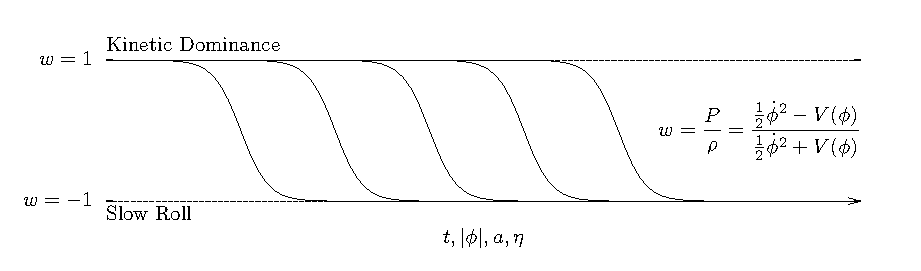
\includegraphics[width=\textwidth]{chapters/kinetic_thoughts/plots/w.tikz}
  \caption{%
    Schematic of the equation of state parameter \(w\) against cosmic
    evolution. The generic scenario entails beginning in a kinetically
    dominated phase with \(w=1\) (i.e.\ \(\dot{\phi}^2\gg V(\phi)\))
    before moving to the typical slow roll attractor solution with
    \(w=-1\) (i.e.\ \(\dot{\phi}^2 \ll V(\phi)\)). We term the
    intermediate stage ``Fast roll''.\label{fig:kt:w}
  }
\end{figure}

The key question is how physically relevant these observations are, and how they relate to more traditional inflationary set-ups and assumptions.

The classical equations have two opportunities to break down. First, it may be that this kinetically dominated state occurs before the Planck time, when we know that we would need a quantum theory of gravity to describe the universe. Second, it may be that the homogeneity assumption breaks down at early times.

\section{The Planck time}
The Planck epoch occurs at the earliest times and is defined as the
regime in which we are certain we would need a quantum theory of
gravity. Effectively this occurs when:
\begin{equation}
  \rho = \frac{1}{2}\dot\phi^2 + V(\phi)  \sim \m^4.
  \label{eqn:kt:rhosim}
\end{equation}
If the universe exits the kinetically dominated solutions before the
Planck time, then kinetic dominance cannot be physically relevant. We
may use this to put bounds on \(\phip\), or alternatively the total
number of \(e\)-folds of inflation.

If we are in the kinetically dominated phase with \(\dot{\phi}^2\gg
V(\phi)\) then:
\begin{equation}
  \rho \approx \frac{1}{2}\dot\phi^2= \frac{1}{3t^2}\m^2 ,
  \label{eqn:kt:rhop}
\end{equation}
so \(\rho\sim\m^4\) implies that \(t\sim\tp=\m^{-1}\). Thus, in order for
kinetic dominance to be true at the Planck time we require that:
\begin{equation}
  V(\phip) \ll \m^4.
\end{equation}
For \(V(\phi) = \frac{1}{2}m^2\phi^2\) inflation, this amounts to requiring that \(m^2\phip^2\ll \m^4\). In order to agree with CMB observations, we require
that \(m\sim10^{-5}\m\), which amounts to requiring that:
\begin{equation}
 \phip^2 \ll 10^{10}\m^2.
 \label{eqn:kt:phipbound}
\end{equation}
We may phrase this in terms of the total number of \(e\)-folds:
\begin{align}
  N_\mathrm{tot} 
  &=\int_{t_\mathrm{begin}}^{t_\mathrm{end}} H dt 
  =\int_{\phi_\mathrm{begin}}^{\phi_\mathrm{end}} 
       \frac{H}{\dot{\phi}}d\phi,  &\text{(\(H=\dot{N}\))}
  \\
  &=\frac{1}{\m^2}\int_{\phi_\mathrm{begin}}^{\phi_\mathrm{end}}
     {\frac{V(\phi)}{V^\prime(\phi)}}d\phi. &\text{(Slow Roll)}
\end{align}
For \(V\sim\phi^n\), this gives:
\begin{equation}
  N_\mathrm{tot} = \frac{\Delta (\phi^2) }{n\:\m^2}.
\end{equation}
If we constrain \(\phi_\mathrm{begin}\) by~\eqref{eqn:kt:phipbound}, and assume that the end of inflation  is somewhere near the base of the potential \(\phi_\mathrm{end}\sim0\), one finds: 
\begin{equation}
  N_\mathrm{tot}\ll 10^{10},
\end{equation}
in order for there to be a pre-inflationary phase after the Planck time.
There is therefore ample room in \(\phi^n\) inflation for a kinetically dominated phase in between the required number of \(e\)-folds of \(N_*\sim50\)--\(60\) and the upper limit somewhere much less than \(10^{10}\). This upper limit agrees with the work of~\cite{how_many_e_folds}, who derive the expected number of \(e\)-folds from a phase-space distribution approach.

It is difficult to imagine how one could possibly constrain the total number of \(e\)-folds observationally, unless the number was sufficiently small so as to be observable directly in the CMB power spectrum, for example in ``just-enough'' inflation by~\cite{Ramirez_excluded_2009,Ramirez_predictions_2012}. For a given inflationary potential, one may place theoretical limits or make predictions on the total number of e-folds \citep{how_many_e_folds}, but these estimates typically tend to be much, much larger than \(50\)--\(60\).

\section{Eternal inflation}
Theorists typically assume an effectively eternal inflationary phase all the way back to the Planck time.  
The typical argument by~\cite{Linde_review} goes something like this:
\begin{enumerate}
  \item We should set initial conditions at the Planck time, when
    \(\rho\sim\m^4\).
  \item There will be some partitioning between kinetic and potential
    energy at this moment.
  \item Given that we know nothing of the physics we should put
    uniform priors the amount of energy in the potential at this
    moment: \(V(\phip)\in[0,\m^4]\).
  \item Therefore, on average we expect equipartition between kinetic
    and potential energy at the Planck time.
\end{enumerate}

From Linde's arguments, the kinetically dominated regime is only present
after the Planck time for \(V(\phip)\) at the very bottom end of the
prior range.

We can see this graphically in Figure~\ref{fig:kt:linde}. Solutions are plotted so that they are equally spaced in kinetic energy at the Planck time. Whilst graphs similar to the upper half of the figure are typically shown in lectures and textbooks, this is for an artificially high value of \(m\). As \(m\) is decreased, the phase space look more like the lower half of Figure~\ref{fig:kt:linde}, and the ``Planck circle'' becomes an elongated ellipse when plotted in \((\phi, \dot{\phi})\) phase space. 

A more modern and concrete encapsulation of Linde's arguments can be seen in~\cite{how_many_e_folds}, where they arrive from phase-space arguments at a prior on the Planck circle of:
\begin{equation}
  \Prob{\theta} = \frac{3}{4} \left|\cos^2\theta\sin\theta\right|,
\end{equation}
with \(\tan\theta  = \dot{\phi}/(m\phi)\), which puts even less weight on the kinetically dominated solutions.

If \(m\) is set to the more physically reasonable \(m\sim10^{-5}\m\), then a prior that is uniform in potential energy puts a lot of weight on extremely large values of \(\phi\). It might be equally reasonable therefore to suggest some kind of logarithmic prior on the value of \(\phi\) at the Planck time, as shown in Figure~\ref{fig:kt:alternate}. In this case, almost by definition, most solutions begin in a kinetically dominated phase.

The problem is that all of these arguments tend to the more philosophical end of physics: ``What is the natural prior to assume on initial conditions?''. It is far better to try and answer these questions observationally. If the kinetically dominated phase is observable, then all of this is moot.

In regards to theory, what we can say with some certainty is that {\em if\/} there is a pre-inflationary phase (significantly after the Planck time) where the physics is still encapsulated by equations~\eqref{eqn:kt:raychaudhuri}~\&~\eqref{eqn:kt:kleingordon}, then that phase must be kinetically dominated. For example, in just-enough inflation \citep{Ramirez_excluded_2009,Ramirez_predictions_2012}, to give consideration to initial conditions one must work in a kinetically dominated phase.





\section{Breakdown of homogeneity}
We have shown that all homogeneous universes classically begin in a kinetically dominated phase. It is profitable to examine the form of the perturbed equations~\eqref{eqn:cos:einsteins_equations_perturb}, to take into account the evolution of any spatial variation in the solutions.

To first order, the \(i\)-\(j\), \(i\)-\(0\) and \(0\)-\(0\) Einstein equations read:
\begin{align}
  \Phi &= \Psi,
  \label{eqn:kt:Eij} \\
  0 &= -\dot{\phi}\:\delta\phi  + 2 H \Phi + 2 \dot{\Phi},
  \label{eqn:kt:Ei0}\\
  0 &= \left(6H^2-\dot{\phi}^2 + 2\frac{k^2}{a^2}\right)\Phi  + \left( -3H\dot{\phi} - \ddot{\phi} \right)\delta\phi + \dot{\phi}\delta\dot{\phi} +  6 H \dot{\Phi},
  \label{eqn:kt:E00}
\end{align}
where we have absorbed the explicit potential dependence into \(\ddot{\phi}\) terms. 
One may rearrange these to gain second order equations in \(\Phi\) or \(\mathcal{R}\):
\begin{align}
  0 &= \ddot{\Phi} + \left( H - 2 \frac{\ddot{\phi}}{\dot{\phi}} \right) \dot{\Phi} + \left( \frac{k^2}{a^2}-\frac{1}{\m^2}\dot{\phi}^2 - 2\frac{\ddot{\phi}}{\dot{\phi}}H \right)\Phi, \\
  0 &= \ddot{\mathcal{R}} + \left( \frac{\dot{\phi}^2}{\m^2H} + 3H + 2\frac{\ddot{\phi}}{\dot{\phi}} \right)\dot{\mathcal{R}} + \frac{k^2}{a^2}\mathcal{R}, \qquad \mathcal{R} = \Psi - \frac{H}{\dot{\phi}}\delta\phi.
\end{align}
There is of course also a second order equation purely in \(\delta\phi\), but this is particularly unappetising, and given that we have an explicit solution for it in~\eqref{eqn:kt:Ei0}, we shall not state it here.
Technically, these equations are derived in the Newtonian gauge (\(E=B=0\)), but since everything here is manifestly gauge invariant one may interpret all of the above equations as the relations in the equivalent gauge invariant variables.

If we apply the kinetically dominated solutions to the background variables, we arrive at:
\begin{align}
  0 &= \ddot{\Phi} + \frac{7}{3}\frac{1}{t}\dot{\Phi} + \frac{k^2}{a^2} \Phi,\\
  0 &= \ddot{\mathcal{R}} + \frac{1}{t}\dot{\mathcal{R}} + \frac{k^2}{a^2} \mathcal{R},\\
  a &\propto t^{1/3}.
\end{align}
Both equations are solvable with Bessel functions as:
\begin{align}
  0 =&\ddot{x} + (1+p)\frac{1}{t}\dot{x} + \frac{k^2}{a^2} x,  \\
  \Rightarrow \qquad
  x =& t^{-\frac{p}{2}}\left[ A J_{\frac{3}{4}p}\left( \frac{3k}{2a} t \right) + B Y_{\frac{3}{4}p}\left( \frac{3k}{2a} t \right) \right], \\
  \sim&  t^{-\frac{p}{2}-\frac{1}{3}}\Bigg[ C \cos\left( \frac{3k}{2a} t -\frac{3p\pi}{8} - \frac{\pi}{4} \right)  \nonumber\\
  &+ D \sin\left( \frac{3k}{2a} t -\frac{3p\pi}{8} - \frac{\pi}{4} \right) \Bigg], \qquad t \gg 1,
\end{align}
where \(A,B,C\) and \(D\) are integration constants. The solutions are generically oscillatory with a polynomial decay with power \(-\frac{p}{2} - \frac{1}{3}\).

Physically that means that as we integrate further backwards in time, although the homogeneous universe is drawn toward a kinetically dominated state, spatial inhomogeneities begin to increase.

Thus, if some portion of the universe at an early stage has \(\dot{\phi}^2 \gg V(\phi)\), and is approximately homogeneous, then evolving forwards in time its homogeneity will tend to increase. Kinetic dominance thus causes patches of the universe to homogenise. This somewhat strengthens the assumption of homogeneity used in the proof of Chapter~\ref{chp:kd}.

Equally, this means that there will be a breakdown in the homogeneity assumption at early times. It remains to be determined at what moment this breakdown occurs for physically observable scales in the early universe. More analytical investigation is required, and is a subject of my current research.


\begin{figure}[tp]
  \centering
  \tikzsetnextfilename{swirl}
  \includegraphics[width=\textwidth]{chapters/kinetic_thoughts/plots/swirl.tikz}
  \tikzsetnextfilename{true}
  \includegraphics[width=\textwidth]{chapters/kinetic_thoughts/plots/true.tikz}
  \caption{Phase-space plot of the evolution of \((\phi,\dot{\phi})\) for a chaotic inflationary potential \(V(\phi) = \frac{1}{2}m^2 \phi^2\). The upper plot has \(m=0.5\m\). The outer circle is the Planck time \(\tp\) when \(\rho=\m^4\). One can see that each path through phase space is generically drawn to the slow roll attractor solutions in the centre of the plot. The lines are plotted so that they have a uniform spacing of kinetic energy at the Planck time.  The upper plot is somewhat misleading, since it has an artificially high value of \(m\). When the value of \(m\) is lowered to \(0.1\m\), as in the lower plot, then the slow roll phase is a much stronger attractor solution, and generates a sustained slow-roll accelerated expansion.}\label{fig:kt:linde}
\end{figure}

\begin{figure}[tp]
  \centering
  \tikzsetnextfilename{swirl_alt}
  \includegraphics[width=\textwidth]{chapters/kinetic_thoughts/plots/swirl_alt.tikz}
  \tikzsetnextfilename{true_alt}
  \includegraphics[width=\textwidth]{chapters/kinetic_thoughts/plots/true_alt.tikz}
  \caption{Phase space plot as in Figure~\protect\ref{fig:kt:linde}, but with initial conditions that are log-uniformly spaced in \(\phi\) at the Planck time. Here, most solutions begin in a kinetically dominated state, whilst still maintaining a sustained inflationary phase.}\label{fig:kt:alternate}
\end{figure}

%
% Reconstructing the primordial power spectrum
% --------------------------------------------
%
\newcommand{\PR}{\mathcal{P}_\mathcal{R}}
\newcommand{\alphamink}{\alpha_\mathrm{min}^{(k)}}
\newcommand{\alphamaxk}{\alpha_\mathrm{max}^{(k)}}
\newcommand{\Pknotj}[1]{\mathcal{P}_{#1}}
\newcommand{\Pknot}{\mathcal{P}}
\newcommand{\As}{A_\mathrm{s}}
\newcommand{\Asj}[1]{A_\mathrm{s}^{(#1)}}
\newcommand{\Nint}{N_\mathrm{int}}
\newcommand{\Nknots}{N_\mathrm{knots}}
\newcommand{\Planck}{\textit{Planck}}


\chapter[PPS reconstruction]{Reconstructing the Primordial Power Spectrum}
\label{chap:rec}

\begin{figure}[tp]
    \tikzsetnextfilename{spline}
    \includegraphics[width=\textwidth]{chapters/pps_reconstruction/plots/spline.tikz}
  \caption{%
    Linear spline reconstruction. The primordial power spectrum is reconstructed using $\Nknots$ interpolation points
    ${\{(k_i,\Pknotj{i}):i=1,2,\ldots {\Nknots}\}}$. The end knots are fixed in $k$ but allowed to
    vary in ${\Pknot}$, whereas the internal knots can vary subject to the constraint that ${k_1<k_2<\cdots<k_{\Nknots}}$.
    The function $\mathcal{P}_\mathcal{R}(k)$ is constructed within the range $[k_1,k_{\Nknots}]$
    by interpolating logarithmically between adjacent knots (i.e., linearly in $\log$-$\log$ space). Outside this range the function is extrapolated logarithmically.
    The function $\mathcal{P}_\mathcal{R}(k;\{k_i,\Pknotj{i}\})$ thus has $2\Nknots-2$ parameters.\label{fig:linear_spline_reconstruction}
  }
\end{figure}



In this section we model the PPS $\PR(k)$ using a nested
family of models where $\PR(k)$ is piecewise linear
in the $\ln (\mathcal{P})$-$\ln (k)$ plane
between a number of knots, $\Nknots$,
that is allowed to vary. The question arises as to how many knots one should use,
and we address this question using Bayesian model comparison.
A family of priors
is chosen where both the horizontal and vertical positions of the knots are allowed
to vary. We examine the ``Bayes factor'' or ``Bayesian evidence'' as a function of
$\Nknots$ to decide how many knots are statistically justified. 
A similar analysis has been performed by~\cite{vazquez_knots} and~\cite{knottedsky1}.
In addition, we marginalize over all possible numbers of knots to obtain 
an averaged reconstruction weighted according to the Bayesian evidence.

The generic prescription is illustrated in Fig.~\ref{fig:linear_spline_reconstruction}. $\Nknots$ knots
$\{(k_i,\Pknotj{i})\,$: $i=1,\ldots,\Nknots\}$ are placed in the $(k,\PR)$ plane and the function $\PR(k)$ is
constructed by logarithmic interpolation (a linear interpolation in $\log$-$\log$ space) between adjacent points.
Outside the horizontal range $[k_1,k_N]$ the function is extrapolated using the outermost interval.

Within this framework, base $\Lambda$CDM arises when ${\Nknots=2}$---in other words, when there are two boundary knots
and no internal knots, and the parameters $\Pknotj{1}$ and $\Pknotj{2}$ (in place of $A_\mathrm{s}$ and $n_\mathrm{s}$) parameterize
the simple power-law PPS\@. There are also, of course,
the four standard cosmological parameters $(\Omega_{\mathrm{b}} h^2$, $\Omega_{\mathrm{c}} h^2$, $100\theta_{\mathrm{MC}}$, and 
$\tau$), as well the numerous foreground parameters associated with the \Planck\ high-$\ell$ likelihood, all of which are unrelated to the PPS\@.
This simplest model can be extended iteratively by successively inserting an additional internal knot, thus requiring with each iteration
two more variables to parameterize the new knot position.


\begin{table}[htbp]
  \centering
  \begin{tabular}{ll}
  Parameter range &
  Prior type
  \\
  \toprule
  \(10^{-4}\,\mathrm{Mpc}^{-1} = k_1< k_2 < \cdots < k_{\Nknots} = 0.3\,\mathrm{Mpc}^{-1}\) &
  log uniform (sorted)
  \\
  \( 2 < \ln\left(10^{10}\Pknotj{1}\right), \ldots ,\ln\left(10^{10}\Pknotj{{\Nknots}}\right) < 4 \)  &
  log uniform
  \\
  \(2\le \Nknots \le 10 \) &
  integer uniform
  \\
  \midrule
  \(0.019< \Omega_\mathrm{b} h^2 <0.025\) &
  uniform
  \\
  \(0.095< \Omega_\mathrm{c} h^2 <0.145\) &
  uniform
  \\
  \(1.03< 100\theta_\mathrm{MC} <1.05\) &
  uniform
  \\
  \(0.01< \tau< 0.4\) &
  uniform
  \\
  \bottomrule
\end{tabular}

  \caption{%
    Prior for moveable knot positions.
    The $\PR$ positions are distributed in a log-uniform manner across a wide range.
    The $k$ positions are also log-uniformly distributed
    across the entire range needed by \CosmoMC{} and are sorted so that ${k_1<\cdots<k_{\Nknots}}$. 
    When we marginalize over the number of knots, $\Nknots$, we assume a uniform prior between 2 and 10.\label{tab:P_k_priors}  }                          % Label goes here.
\end{table}                        % table* is a two-column table.  Drop the * for one column

We run models for a variety of numbers of internal knots, $\Nint =\Nknots -2$, evaluating the evidence for $\Nint$.
Under the assumption that the prior is justified, the most likely, or preferred, model is the one with the highest
evidence.  Evidences are evaluated using the \PolyChord{} sampler \citep{polychordletter,polychordpaper} 
in \CAMB{} and \CosmoMC{}. The use of \PolyChord{} is
essential, as the posteriors in this parameterization are often multi-modal. Also, the ordered log-uniform priors on
the $k_i$ are easy to implement within the \PolyChord\ framework. All runs were performed with $1000$ live points, 
oversampling the semi-slow and fast parameters by a factor of $5$ and $100$, respectively.

\begin{figure}[tp]
  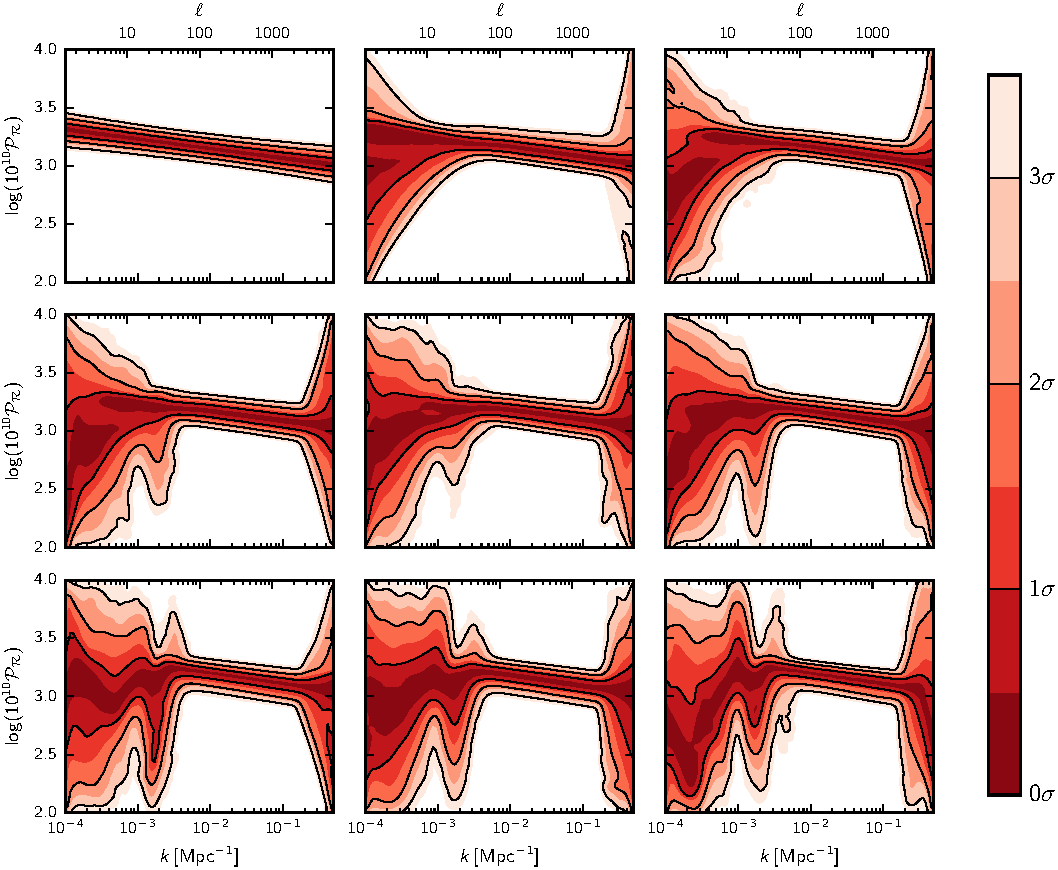
\includegraphics[width=\textwidth]{chapters/pps_reconstruction/figures/array}
  \caption{Bayesian movable knot reconstructions of the primordial power spectrum $\PR(k)$ using \Planck\ TT data.
%{\color{red}[\Planck\ TT+lowP? (JZ)]}
    The plots indicate our knowledge of the PPS $P(\PR(k)|k,N)$ for a given number of knots.
    The number of internal knots $\Nint$ increases (left to right and top to bottom) from $0$ to $8$.
    For each $k$-slice, equal colours have equal probabilities. The colour scale is chosen so that darker regions
    correspond to lower-$\sigma$ confidence intervals.
    $1\,\sigma $ and $2\,\sigma $ confidence intervals are also sketched (black curves).
    The upper horizontal axes give the approximate corresponding multipoles via $\ell \approx k/D_\mathrm{rec}$,
    where $D_\mathrm{rec}$ is the comoving distance to recombination.\label{fig:Pkr0}
  }
\end{figure}


\begin{figure}[tp]
  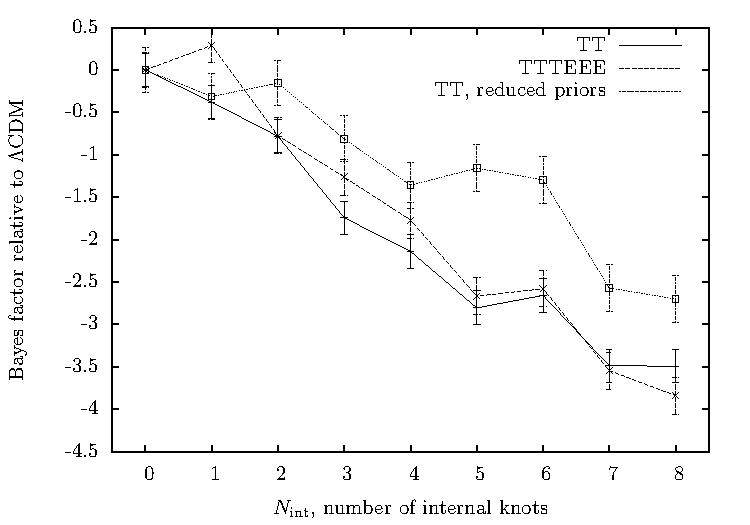
\includegraphics[width=\textwidth]{chapters/pps_reconstruction/figures/Bayes_PR}
  \caption{%
    Bayes factor (relative to the base $\Lambda$CDM model) as a function of the number of knots
    for three separate runs. Solid line: \Planck{} TT\@. Dashed line: \Planck{} TT,TE,EE\@. Dotted line:
    \Planck\ TT, with priors on the $\Pknot$ parameters reduced in width by a factor of 2 ($2.5<\ln(10^{10}\Pknot)<3.5$).\label{fig:Bayes_Factors}
  }
\end{figure}

\begin{figure}[tp]
  \begin{center}
    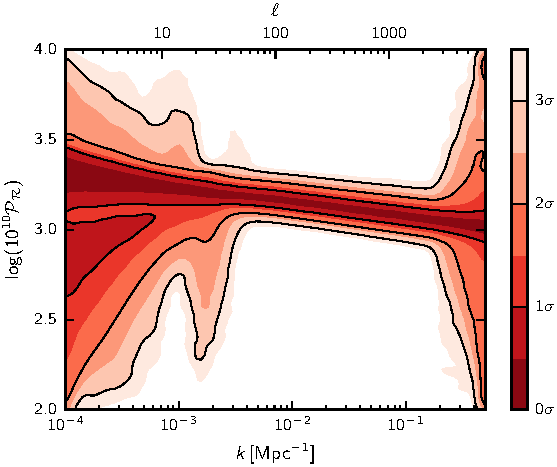
\includegraphics[width=\textwidth]{chapters/pps_reconstruction/figures/single}
  \end{center}
  \caption{%
    Bayesian reconstruction of the primordial power spectrum averaged over different values of $N_\mathrm{int}$
    (as shown in Fig.~\protect\ref{fig:Pkr0}), weighted according to the Bayesian evidence.
    The region ${30<\ell<2300}$ is highly constrained, but the resolution is lacking to say anything precise 
    about higher $\ell$. At lower $\ell$, cosmic variance reduces our knowledge of $\PR(k)$.
    The weights assigned to the lower $\Nint$ models outweigh those of the higher models, so no oscillatory 
    features are visible here.\label{fig:full_bayes_knots}
  }
\end{figure}



Priors for the reconstruction and cosmological parameters are detailed in Table~\ref{tab:P_k_priors}.
We report evidence ratios with respect to the base $\Lambda$CDM case. The cosmological priors remain the
same for all models, and this part of the prior has almost no impact on the evidence ratios.
The choice of prior on the reconstruction parameters
$\{\Pknotj{i}\}$ does affect the Bayes factor. \CosmoMC{}, however, puts an implicit prior on all models by excluding
parameter choices that render the internal computational approximations in \CAMB{} invalid.
The baseline prior for the vertical position of the knots includes all
of the range allowed by \CosmoMC{}, so slightly increasing this prior range will not affect the evidence ratios. If
one were to reduce the prior widths significantly, the evidence ratios would be increased.
The allowed horizontal range includes all $k$-scales accessible to \Planck. Thus, altering this
width would be unphysical.


After completion of an evidence calculation, \PolyChord\ generates a representative set of samples of the posterior for each model
$P(\Theta) \equiv P(\Theta|\mathrm{data},\Nint)$. We may use this to calculate a marginalized probability distribution
for the PPS\@:
\begin{equation}
  P(\log\PR|k,\Nint) = \int \delta\left(\log\PR - \log\PR(k;\Theta)\right)P(\Theta)\:\d{\Theta}.
  \label{eqn:margPR}
\end{equation}
This expression encapsulates our knowledge of $\PR$ at each value of $k$ for a given number of knots.
Plots of this PPS posterior are shown in Fig.~\ref{fig:Pkr0} using \Planck\ TT data.



If one considers the Bayesian evidences of each model, Fig.~\ref{fig:Bayes_Factors} shows that although no model is 
preferred over base $\Lambda$CDM, the case $\Nint=1$
is competitive. This model is analogous to the broken-power-law spectrum of
Sect.~4.4,
although the models differ significantly in terms of the priors used. In this case, the
additional freedom of one knot allows a reconstruction of the suppression of power at low $\ell$. Adding polarization data does not alter 
the evidences significantly, although $\Nint=1$ is strengthened. We also plot a \Planck\ TT run,
%{\color{red}[+lowP? (JZ)]} 
but with the reduced vertical priors ${2.5<\ln\left(10^{10}\Pknot\right)<3.5}$. 
As expected, this increases the evidence ratios, but does not alter the above conclusion.

For increasing numbers of internal knots, the Bayesian evidence monotonically decreases. Occam's razor dictates,
therefore, that these models should not be preferred, due to their higher complexity. However, there is an
intriguing stable oscillatory feature, at $20\lesssim\ell\lesssim50$, that appears once there are enough knots to reconstruct it.
This is a qualitative feature predicted by several inflationary models (discussed in Sect.~9),
and a possible hint of new physics, although
its statistical significance is not compelling.

A full Bayesian analysis marginalizes over all models weighted according to the normalized evidence $Z_{\Nint}$,
so that:
\begin{equation}
  P(\log\PR|k) = \sum\limits_{\Nint} P(\log\PR|k,\Nint) Z_{\Nint},
  \label{eqn:margPR_full}
\end{equation}
%{\color{red}[Define $Z_{\Nint}$. (JZ)]}
as indicated in Fig.~\ref{fig:full_bayes_knots}.
This reconstruction is sensitive to how model complexity is penalized in the prior distribution. 



%
% Defining the quantum vacuum
% ---------------------------
%
\chapter{Defining the Quantum Vacuum}
\label{chp:qv}


\section{Introduction}
\label{sec:qv:introduction}
Traditionally, quantum initial conditions for inflation are set using the Bunch-Davies vacuum. This approach is valid in de Sitter space and other asymptotically static spacetimes. Rapidly evolving spacetimes, however, do not admit such an easy quantisation. 

In Chapter~\ref{chp:kd}, we showed that the classical equations of motion suggest that the universe in fact emerged from the initial singularity in a rapidly evolving state, with the kinetic energy of the inflaton dominating the potential in a pre-inflationary phase. 
This can be used to set initial conditions on the background variables such as the inflaton value and Hubble parameter. 
In order to make contact with real observations, the effect that this phase has on the primordial power spectrum requires a semi-classical quantum mechanical treatment of the comoving curvature perturbation.

Hamiltonian diagonalisation is the simplest approach for setting quantum initial conditions in a general spacetime, and derives the vacuum from the minimisation of the Hamiltonian density. This approach has been criticised in the past as it does not admit a consistent interpretation in terms of particles \citep{Fulling+1989,Fulling_HD}. Other approaches such as the adiabatic vacuum go some way to rescuing the particle concept, but have additional theoretical issues. 

The issue of the particle interpretation stems from an attempt to apply a Minkowski spacetime concept outside the region of its validity.  
We postulate that the minimisation of an energy density is still an appropriate way to define a vacuum. In order to avoid the issues raised against Hamiltonian diagonalisation, we motivate our initial conditions from the minimisation of the {\em renormalised\/} stress-energy density. 
Indeed, if one takes care to minimise the correct quantity (using the theory of quantum fields in curved spacetime), then novel initial conditions can be derived which differ from the traditional Hamiltonian diagonalisation conditions.

After the relevant background material is reviewed, we develop a generic mechanism for setting initial conditions. These reduce to the Bunch-Davies case in asymptotically static spacetimes (such as de Sitter space), but yield different results otherwise. The aim is that these should be more theoretically robust. Additionally, these conditions are potentially distinguishable using observational data.

We then apply this procedure to the kinetically dominated universe, but defer the observational analysis to a later work.



\section{Background}
\label{sec:background}

We denote a general action via:
\begin{equation}
  S_I = \int \d[4]{x}\sqrt{|g|}\mathcal{L}_I,
  \label{eqn:general_action}
\end{equation}
where \(\mathcal{L}_I\) is the {\em Lagrangian density}. We work in natural units \(\hbar=c=1\) and set the reduced Planck mass \(m_\mathrm{p} = {(8\pi G)}^{-1/2} = 1\). Dots denote differentiation with respect to cosmic time \(\dot{f}\equiv \frac{\d{}}{\d{t}}f\), and primes denote differentiation with respect to conformal time \(\prm{f}\equiv\frac{\d{}}{\d{\eta}}f\).

We begin by briefly summarising the classical theory of cosmological perturbations for a general scalar field, before discussing the quantisation of such a theory


\subsection{The classical action}
\label{sec:inflation}
Consider \citep{Baumann+2009} a canonical scalar field \(\phi\) minimally coupled to gravity \(S= S_G + S_\phi\) with:
\begin{equation}
  \mathcal{L}_G = \frac{1}{2}R, 
  \qquad
  \mathcal{L}_\phi = \frac{1}{2}g^{\mu\nu}\nabla_\mu\phi\nabla_\nu\phi - V(\phi).
  \label{eqn:action}
\end{equation}
Extremising this action with respect to the fields \(\phi\) and \(g_{\mu\nu}\) recovers the Klein-Gordon and Einstein equations respectively:
\begin{align}
  \left( g^{\mu\nu}\nabla_\mu\nabla_\nu + \frac{\d{V}}{\d{\phi}} \right) \phi &= 0,
  \label{eqn:klein_gordon}\\
  G_{\mu\nu}\equiv R_{\mu\nu}-\frac{1}{2}g_{\mu\nu}R&= T_{\mu\nu},
  \label{eqn:einstein}
\end{align}
where the stress-energy tensor is:
\begin{equation}
  T_{\mu\nu} = \nabla_\mu\phi \nabla_\nu\phi - \frac{1}{2}g_{\mu\nu} \nabla_\alpha\phi \nabla^\alpha\phi +g_{\mu\nu} V(\phi).
  \label{eqn:SET}
\end{equation}

In cosmology, we assume that at zeroth order both the metric \(g_{\mu\nu}\) and scalar field \(\phi\) are homogeneous and isotropic. Applying these assumptions to equations~\eqref{eqn:klein_gordon}~\&~\eqref{eqn:einstein}, we find:
\begin{align}
  \dot{H}+H^2 &= -\frac{1}{3}\left( \dot{\phi}^2 - V(\phi) \right),
  \label{eqn:Raychaudhuri}\\
  0&=\ddot{\phi} + 3H\dot{\phi} + \frac{\d{V}}{\d{\phi}},
\end{align}
where the Hubble parameter \(H = \dot{a}/a\).
\subsection{Inflationary perturbations}
One then considers scalar perturbations about these background solutions:
\begin{align}
  \phi=&\phi(t) + \delta\phi(t,x),
  \label{eqn:phi_perturbation} \\
  \d{s}^2 =& (1+2\Phi)dt^2 - 2a\partial_i B\d{x_i} \d{t} \nonumber\\
  &-a^2\left( (1-2\Psi)\delta_{ij} + 2\partial_i\partial_j E  \right)\d{x_i} \d{x_j}.
\end{align}
We are interested in the gauge-invariant co-moving curvature perturbation:
\begin{equation}
  \mathcal{R}\equiv \Psi - \frac{H}{\dot{\phi}}\delta\phi,
  \label{eqn:R_action}
\end{equation}
since it is this quantity which defines the primordial power spectrum for seeding cosmological perturbations. Working in the co-moving gauge \(\delta\phi=0\), and expanding the action \(S\) to second order in \(\mathcal{R}\), gives:
\begin{equation}
  S^{(2)} =  \int \d[4]{x} a^3\frac{\dot{\phi}^2}{H^2}{\left[ \dot{\mathcal{R}}^2 - a^{-2} {\left( \partial_i\mathcal{R} \right)}^2 \right]}.
  \label{eqn:S2_action}
\end{equation}
Note that the dependence on \(V(\phi)\) is implicit in the variables \(H,\dot{\phi},a\) and \(\mathcal{R}\).
Defining the Mukhanov variable,
\begin{equation}
  v = z\mathcal{R},\qquad z=\frac{a\dot{\phi}}{H},
  \label{eqn:mukhanov_variable}
\end{equation}
and transforming \(t\) into conformal time \(\eta = \int^t \d{\tau}/a(\tau) \) yields:
\begin{equation}                                 
  S^{(2)} =  \int \d{\eta} \d[3]{x} {\left[ {\left( \prm{v} \right)}^2 - {\left( \partial_i v \right)}^2 + \frac{\dprm{z}}{z} v^2 \right]}.
  \label{eqn:v_action}
\end{equation}
This is the canonically normalised action for a scalar field with time-dependent ``effective'' mass \(\meffs = -\dprm{z}/z\).

\section{Quantisation via Hamiltonian diagonalisation}                                
\label{sec:mukhanov}
We now consider the traditional quantisation of the action~\eqref{eqn:v_action} in spatially flat spacetimes via Hamiltonian diagonalisation. This is a standard method in the inflationary literature, but has several theoretical issues which will be discussed. To begin, one writes;
\begin{equation}
  v = \int \frac{\d[3]{k}}{{(2\pi)}^3} \left[ a_\vk \chi_\vk(\eta)e^{i\vk\cdot\vx} + a_{\vk}^{\dagger} \str{\chi_\vk}(\eta)e^{-i\vk\cdot\vx} \right], 
  \label{eqn:v_quant}
\end{equation}
which expresses the operator \(v\) as a superposition of creation and annihilation operators \(\{a_\vk,a_\vk^\dagger\}\) \citep{Mukhanov+2007}, with the mode functions written in separated form \({u_\vk = \chi_\vk(\eta) e^{i\vk\cdot\vx}}\). If one requires that the scalar field satisfies the equations of motion, along with the canonical commutator relation:
\begin{equation}
  [ a_\vk^{\phantom\dagger}, a_{\prm{\vk}}^{\dagger} ] = {(2\pi)}^3\delta^{(3)}(\vk-\prm{\vk}),
  \label{eqn:commutator}
\end{equation}
holds true, then the temporal part \(\chi_\vk(\eta)\) of the mode functions \(u_\vk\) must satisfy:
\begin{align}
  \dprm{\chi_\vk} + \left( k^2 - \frac{\dprm{z}}{z} \right)\chi_\vk &= 0,
  \label{eqn:mode_mukhanov}
  \\
  \prm{\chi_\vk} \str{\chi_\vk} - \prm{\str{\chi_\vk}} \chi_\vk &= -i.
  \label{eqn:normalisation}
\end{align}
The first of these is the classical equation of motion of the action~\eqref{eqn:v_action}, whilst the second is a normalisation constraint.

\subsection{Choosing a vacuum}
\label{sec:hamiltonian_diagonalisation}
The complex mode functions \(\chi_\vk\) are not fully determined by condition~\eqref{eqn:normalisation}. Although the overall phase of the mode \(\chi_\vk\) is unimportant, there is an additional degree of freedom for each \(\vk\) to be determined. The choice of this is equivalent to choosing a vacuum state \(\ket{0}\), defined by \(a_\vk\ket{0}=0\).

The traditional approach is to consider the Hamiltonian of the Mukhanov variable, which after normal ordering takes the form:
\begin{align}
  H = \frac{1}{2}\int\frac{\d[3]{k}}{{(2\pi)}^3} 
  &\Big[ a_\vk a_{-\vk} F_\vk(\eta) + a_\vk^\dagger a_{-\vk}^\dagger \str{F_\vk}(\eta) \nonumber \\
  &+ \left(2a_\vk^\dagger a_\vk + \delta^{(3)}(0)\right)E_\vk(\eta) \Big], 
\end{align}
where
\begin{align}
  E_\vk(\eta) &= |\chi_\vk^\prime|^2 + \omega_k^2|\chi_\vk|^2,\quad
  F_\vk(\eta) = {\chi_\vk^\prime}^2 + \omega_k^2{\chi_\vk}^2,\\
  \omega_k^2(\eta) &= k^2-\frac{\dprm{z}}{z}.
  \label{eqn:def_omega}
\end{align}
It is therefore attractive to choose either (i) the vacuum as an eigenstate of the Hamiltonian:
\begin{equation}
  H\ket{0}\propto\ket{0} \Rightarrow F_\vk=0,
  \label{eqn:eigenstate}
\end{equation}
or (ii) that the vacuum minimises the expected energy:
\begin{equation}
  \bracket{0}{H}{0} \propto \int \frac{\d[3]{k}}{{(2\pi)}^3} E_\vk.
  \label{eqn:hamil}
\end{equation}
As can be shown with standard linear algebra, these two conditions are equivalent, and result in the requirement that:
\begin{equation}
  |\chi_\vk|^2 = \frac{1}{2\omega_k}, \qquad \prm{\chi_\vk} = -i \omega_k \chi_\vk,
  \label{eqn:hd_condition}
\end{equation}
which provides enough information to set unambiguous initial conditions for the mode equation~\eqref{eqn:mode_mukhanov}.
When the condition~\eqref{eqn:hd_condition} is satisfied, the Hamiltonian is diagonalised such that:
\begin{equation}
  H(\eta_0) = \int\frac{\d[3]{k}}{{(2\pi)}^3} 
  \left(a_\vk^\dagger a_\vk + \frac{1}{2}\delta^{(3)}(0)\right)\omega_k(\eta_0). 
  \label{eqn:diag_hamil}
\end{equation}
We henceforth refer to~\eqref{eqn:hd_condition} as the Hamiltonian diagonalising (HD) vacuum choice.

From~\eqref{eqn:diag_hamil}, one may easily show that \(a_\vk^\dagger\ket{0}\) is a state with energy \(\omega_k(\eta_0)\) and momentum \(\vk\). One therefore traditionally interprets the action of \(a_\vk^\dagger\) at time \(\eta_0\) as creating a ``particle'' from the vacuum. This is a well established interpretation in flat Minkowski space. %In curved spacetime however, we shall see in the following section that this interpretation becomes troublesome.

Note that in general, the conditions~\eqref{eqn:hd_condition} are only satisfied at a specific time \(\eta_0\), and the vacuum is thus a time-dependent notion. 
Indeed, it is straightforward to show that at some different time \(\eta_1\), the expectation \(\bracket{0}{H(\eta_1)}{0}\) of the Hamiltonian in the ground state \(\ket{0}\) is in general larger than the minimum possible value at \(\eta_1\). This is interpreted as the vacuum state \(\ket{0}\) at \(\eta_0\) containing particles at other times \(\eta_1\).

Thus, if one sets these conditions at a time \(\eta_0\), one is effectively setting the universe to be in the vacuum state at that time. The expansion of the universe then excites the vacuum, creating ``particles'' at later times \(\eta_1\). The question as to what is the ``correct'' \(\eta_0\) at which to set these conditions is currently an unresolved theoretical (or indeed observational) issue. 


\subsection{Criticism of Hamiltonian diagonalisation}

Astute readers will have spotted that the expected energy~\eqref{eqn:hamil} is divergent. Whilst the implicit \(\delta^{(3)}(0)\) in the proportionality constant of~\eqref{eqn:hamil} is harmless, and merely accounts for the contribution from the infinite volume of space, there is a second divergence which requires closer attention. For large \(k\), \(E_\vk\sim \omega_k \sim k\), and hence the integral~\eqref{eqn:hamil}, which represents the energy density, is ultraviolet divergent as \(k^4\). 

In traditional quantum field theory, this divergence is subtracted as one only measures energy differences. This is also applicable to spacetimes that are asymptotically static (such as de Sitter space).
However, in changing spacetimes, where the vacuum is time dependent, this subtraction can only be performed at a single instant. If one then advances in time by some finite amount, the space-time generates an infinite particle density \citep{Fulling_HD,Fulling+1989}. 

This is clearly unphysical, causing some authors \citep{Fulling_HD} to discard Hamiltonian diagonalisation as an inappropriate methodology for choosing a vacuum state.

\section{Alternative quantisations}
The particle concept can be somewhat rescued by considering the adiabatic vacuum. This is well defined when the spacetime is changing slowly, as one can then perform an adiabatic expansion. The \(n\)\textsuperscript{th} order adiabatic vacuum at time \(\eta_0\) is defined by matching the general solution of the mode equation~\eqref{eqn:mode_mukhanov} onto the \(n\)\textsuperscript{th} order adiabatic expansion at time \(\eta_0\). This has the satisfying property of more closely corresponding to what a freely falling particle detector would measure, and is generally agreed to be superior to Hamiltonian diagonalisation.

However, there are still some issues with this vacuum. First, it is only usable in slowly changing spacetimes, so only goes halfway to solving the general problem. Second, it introduces a further ambiguity in vacuum choice, namely that of which value of \(n\) to choose. Since the adiabatic expansion is asymptotic, it does not in general converge for large \(n\). One must pick a specific term of the series to truncate at, and there is little theoretical guidance as to what value \(n\) to choose.

We believe that the adiabatic vacuum is in fact trying to rescue the particle concept unnecessarily. A particle interpretation is doomed to failure in general curved spacetime because of the global nature of their definition. Particles are defined in terms of field modes over a large patch of the manifold. Whilst for higher \(\vk\) modes the environment looks effectively Minkowski, low \(\vk\) modes are sensitive to the large scale structure of spacetime.

It would be more sensible to base the notion of a vacuum not in terms of a ``particle-less'' state, but in terms of the minimisation of a {\em local energy density}, such as the \(0\)-\(0\) component of the stress-energy tensor. Unfortunately being quadratic in the field \(\phi\), like the Hamiltonian, \(\bracket{0}{T_{00}}{0}\) is also divergent.

In order to ameliorate this difficulty, we must adopt a more sophisticated approach. 

\section{Quantum fields in curved spacetime} 
\label{sec:QFTCST}
This is the semi-rigorous theory of fields in which gravity is strong enough to generate curvature, but the quantum mechanics only affects spacetime to low order. It can therefore be thought of as a one-loop approximation to quantum gravity.

Traditionally \citep{Birrell+1984,Parker+2009}, one considers a scalar field Lagrangian with mass \(m\), with action:
\begin{equation}
  S = \int \d[4]{x} \sqrt{|g|}\left( \frac{1}{2}g^{\mu\nu}\nabla_\mu\phi\nabla_\nu\phi - \frac{1}{2}m^2\phi^2 \right),
  \label{eqn:scalar_field}
\end{equation}
where for simplicity we are considering the case of minimal coupling \(\xi=0\).  
In the context of FRW spacetime, the modes are quantised as:
\begin{equation}
  \phi(x) = \int\frac{\d[3]{k}}{{(2\pi)}^3a(\eta)} \left[ a_\vk \chi_\vk(\eta)e^{i\vk\cdot\vx} + a_{\vk}^{\dagger} \str{\chi_\vk}(\eta)e^{-i\vk\cdot\vx} \right],
  \label{eqn:mode_expansion}
\end{equation}
where the mode functions are written in separated form \(u_\vk = a{(\eta)}^{-1}\chi_\vk(\eta)e^{i \vk\cdot\vx}\). The additional conformal factor of \({a(\eta)}^{-1}\) generates mode equations without first order derivatives in \(\eta\).
Requiring that the scalar field satisfies the equations of motion, and that the commutation relation~\eqref{eqn:commutator} remains true,
one finds that the mode functions \(\chi_\vk\) must satisfy:
\begin{align}
  \dprm{\chi}_\vk + \left[ k^2 + a^2 m^2 - \frac{\dprm{a}}{a}  \right] \chi_\vk &= 0,
  \label{eqn:chi_equation}\\
  \prm{\chi_\vk} \str{\chi_\vk} - \prm{\str{\chi_\vk}} \chi_\vk &= -i.
  \label{eqn:normalisation_1}
\end{align}

\subsection{Application to inflation}
\label{sec:bridge}
The similarity between equations~\eqref{eqn:mode_mukhanov} and~\eqref{eqn:chi_equation} is striking. It suggests solving for the quantum curvature perturbation is equivalent to solving a massless scalar field in an alternative spacetime with scale factor satisfying:
\begin{equation}
  \frac{\dprm{a}}{a} = \frac{\dprm{z}}{z}.
  \label{eqn:mapping}
\end{equation}
This may be explicitly solved for \(a(\eta)\) as:
\begin{equation}
  a(\eta) = A\:z(\eta) + B\:z(\eta) \int^\eta \frac{\d{x}}{{z(x)}^2},
  \label{eqn:a_sol}
\end{equation}
where \(A\) and \(B\) are constants of integration. 

Considering the special case of the inflating universe; during inflation \(H\) and \(\dot{\phi}\) are approximately constant, so \(z\propto a\), as in the exact de Sitter case. Thus, quantising the Mukhanov variable during inflation is equivalent to quantising a massless, minimally coupled scalar field on the same background spacetime. Note however, that in a more general scenario, the two spacetimes will not be the same.

\section[Minimising the renormalised SET]{Minimising the renormalised stress-energy tensor}
Within the theory of quantum fields in curved spacetime, one is able to compute a {\em renormalised\/} stress-energy tensor \(\bracket{0}{T_{\mu\nu}}{0}_\mathrm{ren}\). There are a variety of methods of doing this, but if carried out carefully they yield the same result.

\subsection{Hadamard point splitting}
We briefly recap the procedure for evaluating a renormalised stress-energy tensor via a Hadamard point splitting procedure.  
The Hadamard Green function is defined by:
\begin{equation}
  G^{(1)}(x,\prm{x}) =\frac{1}{2} \bracket{0}{\left\{ \phi(x),\phi(\prm{x}) \right\}}{0}.
  \label{eqn:green_function}
\end{equation}
The coincidence limit \(\prm{x}\to x\) formally would yield the expectation \(\bracket{0}{\phi^2}{0}\), but this is unfortunately divergent. The strategy therefore is to subtract off de-Witt Schwinger geometrical terms \(G^{(1)}_\mathrm{DS}(x,\prm{x})\) which may be absorbed into a renormalisation of the ``bare'' constants \(G_B\) and \(\Lambda_B\). One then takes the coincidence limit to yield a non-divergent quantity. 

To form the stress-energy tensor from the Green function, one operates with a bi-scalar derivative function \(D_{\mu\nu}(x,\prm{x})\):
\begin{align}
  \bracket{0}{T_{\mu\nu}(x)}{0}_\mathrm{ren} =& \lim\limits_{\prm{x}\to x} \mathcal{D}_{\mu\nu}(x,\prm{x}) \left[ G^{(1)}(x,\prm{x}) - G^{(1)}_\mathrm{DS}(x,\prm{x}) \right],
  \label{eqn:point_splitting}
  \\
  \mathcal{D}_{\mu\nu}(x,\prm{x})=& \frac{1}{2}\left( \nabla_{\mu}\nabla_{\prm{\nu}} + \nabla_{\prm{\mu}}\nabla_{\nu} \right) -\frac{1}{2} g_{\mu\nu} \nabla_\alpha \nabla^{\prm{\alpha}} \nonumber\\
  &+ g_{\mu\nu} \frac{1}{2}m^2  \nonumber,
\end{align}
where, as we are taking the coincidence limit, the metric \(g_{\mu\nu}\) may be evaluated at either \(x\) or \(\prm{x}\).
The Hadamard Green function~\eqref{eqn:green_function} using the mode expansion~\eqref{eqn:mode_expansion} becomes:
\begin{align}
  G^{(1)}(x,\prm{x}) = 
  \int\frac{\d[3]{k}\:}{{(2\pi)}^3a(\eta)a(\prm{\eta})}&
  \Big(
  \chi_\vk(\eta)
  \str{\chi_{\vk}}(\prm{\eta})e^{i\vk\cdot(\vx-\prm{\vx})}+\nonumber\\
  &
  \str{\chi_\vk}(\eta)
  \chi_{\vk}(\prm{\eta})e^{-i\vk\cdot(\vx-\prm{\vx})}
  \Big)
  \nonumber.
\end{align}
Inserting this expression into~\eqref{eqn:point_splitting} will yield an expression which depends on the specific choice of mode function \(\chi_\vk\). We now regard this expression as a {\em functional\/} of the independent variables:
\begin{equation}
  \mathcal{X} = \{\chi_\vk,\str{\chi_\vk},\prm{\chi_\vk},\prm{\str{\chi_\vk}}\},
  \label{eqn:vars}
\end{equation}
and aim to minimise this with respect to the functions. Since \(G^{(1)}_{\mathrm{DS}}\) does not depend on these variables, this term can be ignored for the purposes of extremisation. Further, the functional derivatives such as \(\frac{\delta}{\delta \chi_\vk}\) commute with the limit expression, so in fact minimising the renormalised tensor with respect to the mode functions is equivalent to na\"{\i}vely minimising the traditional stress-energy tensor~\eqref{eqn:SET}. Inserting the mode function~\eqref{eqn:mode_expansion} into~\eqref{eqn:point_splitting} and taking the coincidence limit, one finds:
\begin{align}
  \bracket{0}{T_{00}(x)}{0}_\mathrm{ren} = &\frac{1}{2}\int \frac{\d[3]{k}}{{(2\pi)}^3 a^2} \Big[ (\prm{\chi_\vk}-\frac{\prm{a}}{a}\chi_\vk)(\prm{\str{\chi_\vk}}-\frac{\prm{a}}{a}\str{\chi_\vk})
  \nonumber \\
  &+\left( k^2 + m^2a^2 \right)\chi_\vk {\chi_\vk}^\ast + \tilde{T} \Big],
\end{align}
where \(\tilde{T}\) signifies the plethora of additional terms arising from the renormalisation process that have no dependence on the variables \(\mathcal{X}\).
Minimising this with respect to \(\mathcal{X}\) subject to the constraint~\eqref{eqn:normalisation_1} yields the relations:
\begin{align}
  |\chi_\vk|^2 &= \frac{1}{2\sqrt{k^2+m^2a^2}}, \\
  \prm{\chi_\vk} &= \left( -i \sqrt{k^2+m^2a^2} + \frac{\prm{a}}{a} \right) \chi_\vk.
  \label{eqn:rn_condition_m}
\end{align}


\subsection{Application to the Mukhanov variable.}
Recalling Section~\ref{sec:bridge}, to apply this formalism to the Mukhanov variable, one should set \(m=0\) and replace \(a\) with \(z\):
\begin{equation}        
  |\chi_\vk|^2 = \frac{1}{2k},\qquad
  \prm{\chi_\vk} = \left( -i k + \frac{\prm{z}}{z} \right) \chi_\vk.
  \label{eqn:rn_condition}
\end{equation}
This should now be compared with the more usual HD conditions~\eqref{eqn:hd_condition}. Deep inside the horizon (\({k\gg -{\prm{z}}/{z}}\)) these two initial conditions are equivalent, but yield very different answers for infra-red modes (small \(k\)).
The second of these equations may be re-written in a more illuminating form:
\begin{equation}
  \prm{\left( \frac{\chi_\vk}{z} \right)} = -i k \left( \frac{\chi_\vk}{z} \right),
\end{equation}
which suggests that the co-moving curvature \(\mathcal{R}=v/z\) is set with a ``positive frequency mode'' independent from any spacetime variation.

It is important to recognise setting these conditions at \(\eta_0\) is equivalent to forcing the universe into a vacuum state at that moment, but there is minimal theoretical guidance as to when this should be\footnote{Although~\protect\cite{Lasenby2009} has suggested using successive adiabatic approximations to pick the vacuum epoch as the moment when the field is most ``particle-like''.}. Indeed, there is little reason to imagine that the universe should be in a vacuum state at any given moment. However, these conditions could also be used to build a formalism of excited states.

It is also important to realise that this vacuum does not claim to be interpretable in terms of particles. It is merely the mode function that minimises the renormalised stress tensor. In the language of Hamiltonian diagonalisation, or adiabatic vacuums, it would be a superposition of ``particle states''.

\cite{vacuum_choice} provides a review (particularly in the appendix) of various choices of initial conditions analogous to~\eqref{eqn:hd_condition} and~\eqref{eqn:rn_condition}. It is interesting to note that the~\cite{Danielsson} vacuum bears a striking similarity to the renormalisation initial conditions~\eqref{eqn:rn_condition} we have derived. The~\cite{Danielsson} vacuum \citep[also discussed by][]{Danielsson2} is instead derived from phenomenological grounds by imposing initial conditions around a high energy cutoff.

\section{Renormalising the KD universe}
\begin{figure}[tp]
  \centering
  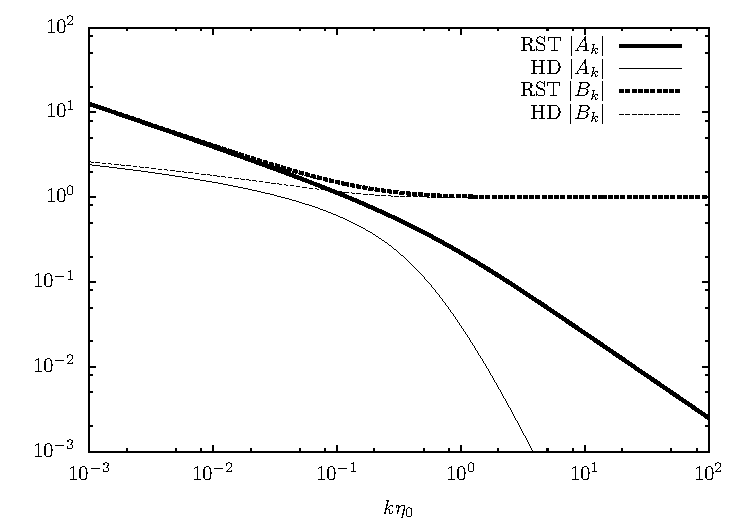
\includegraphics[width=\columnwidth]{chapters/quantum_vacuum/figures/Ak.pdf}
  \caption{The modulus of the \(A_k\) and \(B_k\) coefficients in a kinetically dominated universe for the Hamiltonian diagonalising vacuum~(HD) and the vacuum from the renormalised stress tensor~(RST). Under these conditions, the universe will be in a vacuum state at conformal time \(\eta_0\). Note that at large \(k\), the mode functions tend to \(A_k=0\), \(B_k=1\).}\label{fig:Ak}
\end{figure}
We now consider these observations in the context of the kinetically dominated universe. 
As is detailed in Chapter~\ref{chp:kd} \citep[and in][]{Handley+2014}, the classical solutions to the evolution equations~\eqref{eqn:klein_gordon}~\&~\eqref{eqn:Raychaudhuri} emerge almost always from a kinetically dominated phase with \(\dot{\phi}^2\gg V(\phi)\). 
In this regime, there is a significant period of cosmic time in which the theory of Section~\ref{sec:QFTCST} is valid. 
In this semi-classical pre-inflationary context, one finds that \(\dot{\phi}\propto H\) and hence \({z\propto a}\). 
In the same manner as a de Sitter universe, quantising the co-moving curvature perturbation is equivalent to quantising a massless scalar field on the same background spacetime. 
In this case though, the scale factor \({a \propto \eta^{1/2}}\), so the mode equations have the general solution:
\begin{align}
  \chi_\vk(\eta) &= \frac{1}{2}\sqrt{\pi\eta}\left( A_k H_{0}^{(1)}(k\eta) + B_k H_{0}^{(2)}(k\eta) \right) \nonumber, \\
  1&=|B_k|^2 - |A_k|^2, \label{eqn:kd_modes} 
\end{align}
where without loss of generality we assume \(A_k\) is real.
Applying HD conditions~\eqref{eqn:hd_condition}, or our new renormalised stress tensor conditions~\eqref{eqn:rn_condition} yields different values for \(A_k\) and \(B_k\), as indicated in Figure~\ref{fig:Ak}. This difference is potentially observationally distinguishable, and will be analysed in a following paper.


\section{Conclusions}
We have presented a novel procedure for setting the initial conditions on the Mukhanov-Sazaki equation. We define the vacuum state via the instantaneous minimisation of the renormalised stress-energy tensor. This procedure is valid for any background cosmology, independent of the thorny issue of a particle-type concept. It reduces to the Bunch-Davies vacuum in an asymptotically static region. Further, it makes theoretical predictions that may be observationally testable.





%
% Kinetic initial conditions for inflation
% ----------------------------------------
%
%\chapter{Kinetic Initial Conditions for Inflation}
\label{chap:ic}

\section{Introduction}
\label{sec:ic:intro}

%
\chapter*{Conclusion: Part~\ref{part:cosmology}}
\addcontentsline{toc}{chapter}{Conclusion: Part~\ref{part:cosmology}}
\markboth{Conclusion: Part~\ref{part:cosmology}}{Conclusion: Part~\ref{part:cosmology}}

This part began by showing in Chapter~\ref{chap:kd} that almost all classical inflationary solutions begin in a generic kinetically dominated phase. The generality of this statement was discussed in Chapter~\ref{chap:kt}. 
Whether or not this phase occurs in reality can only be established by observation. If inflation was sufficiently short, then this pre-inflationary epoch may be observable as a suppression in power at low-$\ell$ in the $C_\ell$ spectrum, or in low-$k$ in the $\mathcal{P}_\mathcal{R}(k)$ spectrum. 

In Chapter~\ref{chap:rec}, I showed that if one reconstructs the primordial power spectrum $\mathcal{P}_\mathcal{R}(k)$ from a Bayesian perspective there is some weak evidence for a suppression of power at low-$k$, as well as an anomaly at $\ell\sim30$. Whilst this by no means provides evidence for an observable kinetically dominated epoch, it does suggest the possibility that with better data there could be.

In order to gain more theoretical guidance on the precise predictions which the kinetically dominated universe makes about the primordial power spectrum, we have to gain a greater understanding of the quantum mechanics of this phase. The details of this are non-trivial, since as soon as one migrates away from a de-Sitter limit, the theory as to how to set initial conditions becomes far more murky. Chapter~\ref{chap:qv} has enumerated some of these issues, and provided an alternative possibility for quantising a kinetically dominated universe.

\section*{Future work}
\subsection*{Theoretically investigating kinetically dominance}
The results of Chapter~\ref{chap:kt} require further investigation. In particular, since linear spatial perturbations grow backwards in time, the universe is more inhomogeneous closer to $t=0$. This will lead to a breakdown in the assumptions at some point, and it would be helpful to quantify this fully. In particular, it would useful to know if the breakdown is earlier than the Planck scale for $k$-scales of observational interest.

Further, since the kinetically dominated universe stabilises forwards in time, it would be interesting to quantify how generic our initial conditions are, and whether a homogeneous kinetically dominated phase naturally arises for any universe beginning with $\dot{\phi}^2\gg V(\phi)$. This would involve similar machinery to that used in ``eternal inflation'' scenarios.


\subsection*{Constraining the kinetically dominated universe}

The next task would be to ask if the data can provide any further insight into the quantum vacuum of the kinetically dominated universe. It would be particularly interesting to find out if the data themselves were capable of distinguishing between vacua. This could be done for the current set of cosmological data, or one could ask about the feasibility of future data sets in providing constraints on this portion of the unierse.

A full analysis would involve numerically integrating the quantum mechanical equations through the pre-inflationary phase all the way to horizon exit. Since these equations are highly oscillatory with time-varying coefficients, this would require a numerical method capable of tackling these. In fact, I have begun work on such a technique, which is detailed in Chapter~\ref{chap:RK}.

If one of these vacua is the ``correct'' one, it still remains to be determined when, if at all, it was in its vacuum state. It may be that we can provide observational constraints on the precise value of this moment.

\subsection*{Further constraints on inflation}
In addition, as a member of Planck core team II, I intend to continue more traditional observational reconstructions of inflationary and cosmological functions.

In general, inflationary analysis begins with the definition of the potential $V(\phi)$. This then predicts a primordial power spectrum $\mathcal{P}_\mathcal{R}(k)$ via a numerical integration of the Mukhanov-Sazaki (MS) equations. The primordial power spectrum is then converted via cosmological transfer functions ($\Delta$) into a set of multipole moments:

\tikzsetnextfilename{inflation_procedure}
\begin{center}
  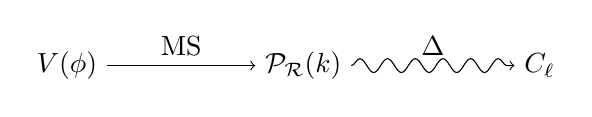
\begin{tikzpicture}[decoration=snake]
    \draw[] (3,0) node (Cl) {$C_\ell$};
    \draw[] (0,0) node (Pr) {$\mathcal{P}_\mathcal{R}(k)$};
    \draw[] (-3,0) node (Vphi) {$V(\phi)$};
    \draw[->,decorate] (Pr) -- (Cl) node[midway,above]{$\Delta$};
    \draw[->] (Vphi) -- (Pr) node[midway,above]{MS};
  \end{tikzpicture}
\end{center}

In Chapter~\ref{chap:rec} we applied a Bayesian reconstruction procedure to the middle stage, and reconstructed the primordial power spectrum in a model independent manner.  
We intend to apply our Bayesian reconstruction procedure separately to all three of these stages of the analysis, with the new updated polarisation data.

%\subsubsection{Primordial power spectrum $\mathcal{P}_\mathcal{R}(k)$ reconstruction}
%This would be much the same as in the 2015 paper, with possibly a little more investigation into prior sensitivities, and obviously updated to use the new polarisation data.
%
%\subsubsection{Inflationary potential $V(\phi)$ reconstruction}
%Here we would parameterise the inflationary potential $V(\phi)$ with movable knots. In addition, we will require the e-folding of the pivot scale $50<N_*<60$ to be a free parameter to be fitted. This avoids any difficulties with re-heating parameterisations.
%To avoid ``ringing'' effects in the subsequent primordial power spectrum, we will probably use a cubic rather than linear spline. We will also put a fairly strong prior on the potential; 
%\begin{itemize}
%  \item Inflation must finish at $\phi=0$. This can be achieved by setting $V=\frac{d}{d\phi}V = 0$ at $\phi=0$.
%  \item The potential must support at least $50-60$ e-folds of inflation, with a continuous inflationary phase in between $\phi=\phi_*$ and $\phi=0$.
%\end{itemize}
%For this reason, it is essential that we provide plots of the prior $V(\phi)$ as well as the posterior.
%
%The horizontal prior on the $\phi$-co\"{o}rdinates of the knots will be linear, whilst the prior on the vertical position will be either logarithmic or linear (we will attempt both).
%
%\subsubsection{Multipole moment $C_\ell$ reconstruction}
%Here, the aim is to move the reconstruction to the other end of the analysis, and probe the significance of the anomalies (if any) that have been appearing in the $C_\ell$ spectrum. 
%
%The Planck likelihoods may be thought of as functions of the theoretical multipole moments $C_\ell^\mathrm{\Lambda CDM}$, which are in turn functions of the $\Lambda$CDM cosmological parameters $\Theta$:
%\begin{equation}
%  \mathcal{L} = \mathcal{L}(C_\ell), \qquad C_\ell = C_\ell^{\mathrm{\Lambda CDM}}(\Theta)
%\end{equation}
%  
%  Our plan is to parameterise the theoretical $C_\ell$'s with an additional reconstructed alteration:
%\begin{equation}
%  C_\ell = C_\ell^\mathrm{\Lambda CDM}(\Theta) + \delta C_\ell(\Psi),
%\end{equation}
%where $\Psi$ are a set of reconstruction parameters for the unknown function.
%
%Priors on the $\delta C_\ell$ and $\ell$ components of the knots will have to be considered carefully, but a parameterisation that is linear in $\ell(\ell+1)\delta C_\ell$ and $\ell$ seems a reasonable start. We may also need to discretise the $\ell$-positions of the knots. There is nothing about our analysis (or \PolyChord{}) that precludes this option. 
%
%It would also be useful to see the equivalent plots of Figure~\ref{fig:full_bayes_knots} for the $C_\ell$'s in comparison to their observed values and errors.
%
%One particularly powerful aspect of this parameterisation, is that the $\delta C_\ell$ adjustment occurs post-transfer function calculation. This means that $\Psi$ are effectively ``fast parameters'', and we can therefore potentially add a great many of these before incurring a computational cost.
%
%
%
\cleardoublepage{}

%
%
%
% Methods
% =======
%
\part{Methods}
\label{part:statistics}
%
% Bayesian inference
% ------------------
%
\chapter{Bayesian Inference}
\label{chap:bay}
%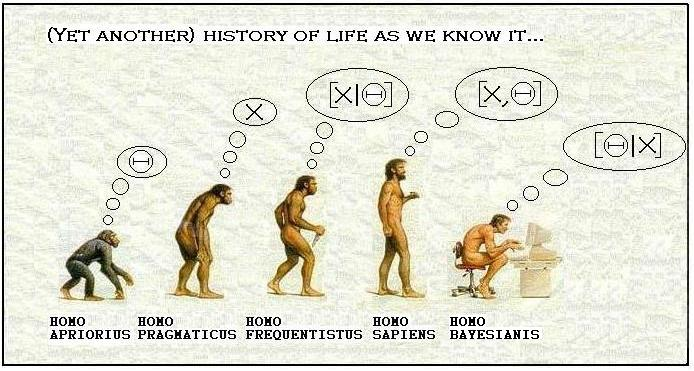
\includegraphics[width=\textwidth]{chapters/bayesian_inference/figures/bayesian_evol}

\epigraph{We anticipate the sun will rise tomorrow, not just because it has always done so far, but because this is predicted by {\em models}, which accord with {\em data}. Any perceived failure of the sun to rise would more likely be a hallucination.}{\davidmackay{}}

Despite popular conception, science is not the search for truth. Scientists instead concern themselves with the construction descriptive and predictive models that have their relative merit determined using data.
The natural language to encapsulate these ideas is that of Bayesian probability. This chapter reviews the concepts and notation of this ``meta-science''.

\section{Probability}
\label{sec:bay:prob}

Probability is the mathematical language of uncertainty. 
A numerical weighting is assigned to all events, which roughly corresponds to the ``chance'' that such an event would occur. An event \(E\subset \Omega\) is defined as a subset of all possible outcomes \(\Omega\). Probability is defined as being additive over the set of all possible events, such that:
\begin{equation}
  A\cap B = \phi \Leftrightarrow \text{\(A\), \(B\) disjoint} \Leftrightarrow \Prob{A} + \Prob{B} = \Prob{A\cup B}.
\end{equation}
\johnskilling{} has derived these properties of probability from measurement-theoretical grounds~\citep[chap. 1]{Bayesian_methods_in_cosmology}, which provides a more intuitive backing to the standard Kolmogorov axioms.

\subsection{Bayes' theorem}

\begin{figure}[tp]
  \centering
  \tikzsetnextfilename{bayes_theorem}
  \includegraphics[width=\textwidth]{chapters/bayesian_inference/plots/bayes_theorem.tikz}
  \caption{Diagrammatic Bayes' theorem. Nodes indicate the occurrence of an event. Edges indicate the probability of an event occurring, and are multiplicative in the direction of the arrows. Bayes' theorem~\protect\eqref{eqn:bay:bayes} may be derived by equating the path \(A\to A\cap B\) with \(A\to\Omega\to B\to A\cap B\).}\label{fig:bay:bayes_theorem}
\end{figure}


The conditional probability of event \(B\) given event \(A\) is defined via:
\begin{equation}
  \Probc{B}{A} = \frac{\Prob{A\cap B}}{\Prob{A}}.
  \label{eqn:bay:cond}
\end{equation}
Multiplying both sides by \(\Prob{A}\), and noting the symmetrical alternative:
\begin{equation}
  \Probc{B}{A}\Prob{A} = \Prob{A\cap B} = \Probc{A}{B}\Prob{B},
  \label{eqn:bay:sym}
\end{equation}
one may then derive Bayes' theorem:
\begin{equation}
  \Probc{B}{A} = \frac{\Probc{A}{B}\Prob{B}}{\Prob{A}}.
  \label{eqn:bay:bayes}
\end{equation}
Bayes' theorem indicates how to reverse the conditionality in a probability distribution \(\Probc{A}{B}\): one first deconditions by multiplying by \(\Prob{B}\) and then reconditions via the normalising constant \(\Prob{A}\). Figure~\ref{fig:bay:bayes_theorem} extends this to all possibilities for two events.
With the algebra of conditionals, probability is the only measurable quantity with both a closed multiplication and addition.

\section{Bayesian vs.\ Frequentist}
\label{sec:bay:bayesian_frequentist}

There are two fundamental types of probability: {\em Aleatoric\/} and {\em Epistemological}. Aleatoric systems are genuinely random, for example: the flip of a coin, or the click on a Geiger counter. Epistemological probability governs systems where the randomness is associated with a subjective lack of knowledge. 

Along with this, there are two interpretations of probability and the meaning of chance; {\em Bayesian\/} and {\em Frequentist}.\footnote{Personally, I disapprove of this terminology. I prefer the terms ``correct'' and ``unhelpfully restrictive''.}
The Frequentist school of thought defines probability as:
\begin{description}
  \item[Frequentist Probability:]``The limiting relative frequency of an event.''
\end{description}
If a coin has \(\Prob{\mathrm{Head}}=\frac{1}{2}\), then if you were to toss it an arbitrarily large number of times, the fraction of events that are heads would get closer and closer to \(\frac{1}{2}\). This is the version of probability that most people encounter early in their mathematical education. 

This definition applies relatively well to Aleatoric systems (since an experiment can often be run a large number of times). However, for epistemological systems, it is all but useless. The frequentist solution is therefore to disregard the latter kind of probability.

For example, most people's experiences with probability will likely involve betting scenarios. For example, before prince George was born, bookmakers took bets on whether William and Kate's baby was a boy or a girl. Here it is obvious that the betting odds should be approximately \(50:50\),\footnote{Betting odds of \(a:b\) against indicates a probability of success of \(\frac{b}{a+b}\).}\footnote{In fact the probability of a boy being conceived across the population is roughly 51\%, in order to biologically account for male infant mortality. An individual's probability of conceiving a boy or a girl will vary from person to person and in time.}\footnote{A good bookmaker will obviously take this into account, and give you slightly worse odds in order to ensure their profit.} but it should be also be clear that these odds do not refer to an event that can be repeated an arbitrarily large number of times.

The alternative definition of probability is {\em Bayesian\/}:
\begin{description}
  \item[Bayesian Probability:] ``A degree of belief that an event will occur.'' 
\end{description}
Note that Bayesian probability is {\em subjective}, it matters who's degree of belief one is considering. Probabilities are assigned only with a given state of knowledge. Effectively, Bayesians place aleatoric and epistemological probability under the same umbrella. 

Pure mathematics deals in relative truth or falsity, i.e.\ given initial assumptions, all statements are assigned to the set \(\{F,T\}\equiv\{0,1\}\). Bayesian probability can be thought of as a blurring of this process, namely from initial assumptions, various conclusions are assigned a number from the continuum between \([0,1]\).

\section{An example: biased coins}
As an concrete introduction to the terminology, we will consider the case of determining whether a coin is biased.
For example, assume that you toss a coin \(N=20\) times, and observe a dataset of \(\data = 16\) heads. Is this enough to cause us to doubt the fairness of the coin?

The standard model \(\model_0\) is that a coin toss consists of a binomial trial with probability \(\frac{1}{2}\). Elementary probability tells us that the chance of getting this data is:
\begin{equation}
  \Probc{\data}{\model_0}= {^{N}C_\data} {\left( \frac{1}{2} \right)}^{N}  = 4.6\times 10^{-3}.
  \label{eqn:bay:M0}
\end{equation}
Note that as should be expected, the chance of obtaining this exact dataset is small. 

If we allow for the possibility that the coin could be any probability \(p\), we can encapsulate this in a second model \(\model_1\).
\begin{equation}
  \Probc{\data}{p,\model_1}= {^{N}C_\data}\: {p}^{\data} {\left(1 - p \right)}^{N-\data}.
  \label{eqn:bay:M1}
\end{equation}
This second model is not ideal, since we haven't specified the parameter \(p\). If we choose \(p=\frac{1}{2}\) we recover \(\model_0\). It is tempting to choose \(p\) such that the probability of getting the data is maximised. This would be an example of a {\em maximum likelihood\/} approach. In this case, the method indicates\footnote{Proof left as exercise to the reader.} we should choose \(p = \frac{\data}{N}\). 

Maximum likelihood has its drawbacks, particularly in the case of a low volume of data. After \(N=1\) toss, it seems a little premature to choose either \(p=1\) or \(p=0\) depending on whether we see a head or a tail. Instead picking a specific value of \(p\), one could instead ``spread your bets'' and consider several different values of \(p\). The full generalisation of this is to consider a continuum of models, and define an initial probability distribution on \(p\), \(\Probc{p}{\model_1}\). This can be interpreted as our initial assumptions on the value of \(p\), or our initial degree of belief in its value.
A natural assumption is to try and be as unbiased as possible and assume that \(p\) is equally likely to take any value in between \(0\) and \(1\). We therefore have:
\begin{equation}
  \Probc{p}{\model_1}=\left\{
  \begin{array}{lr}
    1 &:0\le p\le1\\
    0 &:\text{otherwise.}\\
  \end{array}
  \right.\label{eqn:bay:prior1}
\end{equation}
With this distribution, we can work out what the overall probability of obtaining the dataset \(\data\) is, by marginalising over all values of \(p\):
\begin{align}
  \Probc{\data}{\model_1} 
  &= \int \Probc{\data}{p,\model_1}\Probc{p}{\model_1}\: \d{p}, \\
  &= \int_0^1 {^{N}C_\data}\: {p}^{\data} {\left(1 - p \right)}^{N-\data}\: \d{p}, \\
  &= \frac{1}{n+1} = 4.8\times10^{-2}.
  \label{eqn:bay:marg}
\end{align}
This is quite telling, because our initial choice~\eqref{eqn:bay:prior1} for \(\Probc{p}{\model_1}\) indicates that we expect all data sets with equal probability (independent of \(\data\)). This is therefore a ``minimally suspicious'' choice in spread.

We now have two equations~\eqref{eqn:bay:M0}~\&~\eqref{eqn:bay:marg} which detail the probability of getting the dataset \(\data\) given the choice of model. However, what we are really after is the probability of the model, given the dataset \(\Probc{\model}{\data}\). To compute this, we use Bayes' theorem:
\begin{equation}
  \Probc{\model}{\data} = \frac{\Probc{\data}{\model}\Prob{\model}}{\Prob{\data}}.
  \label{eqn:bay:bay_md}
\end{equation}
In order to complete the calculation, we must assign a probability to each model. A natural choice is to consider \(\Prob{\model_0}=\Prob{\model_1}=\frac{1}{2}\). \(\Prob{\data}\) is just a normalising constant, computed as:
\begin{equation}
  \Prob{\data} = \sum_i \Probc{\data}{\model_i}\Prob{\model_i}, 
  \label{eqn:bay:norm}
\end{equation}
so we may finally compute:
\begin{equation}
  \Probc{\model_0}{\data} = 0.088, \qquad
  \Probc{\model_1}{\data} = 0.922.
  \label{eqn:bay:comp}
\end{equation}
In other words, a betting man would give the odds of the coin being unbiased \(\model_0\) as approximately \(10:1\). Another way of thinking of this is that \(\model_1\) is ten times better at describing the data than \(\model_0\).

\(\model_1\) can go further however. We may also use Bayes' theorem to compute:
\begin{equation}
  \Probc{p}{\data,\model_1} = \frac{\Probc{\data}{p,\model_1}\Probc{p}{\model_1}}{\Probc{\data}{\model_1}}.
  \label{eqn:bay:bay_p}
\end{equation}
This here gives us the distribution on \(p\) {\em given the data}. Namely, how the data should update our ``spread bet''. We already have the ingredients for the above construction from equations~\eqref{eqn:bay:M1},~\eqref{eqn:bay:prior1},~\&~\eqref{eqn:bay:marg}, and given the uniform prior, we find our updated bet on \(p\) is proportional to \(p^\data{(1-p)}^{N-\data}\), a function of \(p\). This is a beta distribution, and is indicated in Figure~\ref{fig:bay:beta}.

\begin{figure}[tp]
  \centering
  \tikzsetnextfilename{beta_function}
  \includegraphics[width=\textwidth]{chapters/bayesian_inference/plots/beta_function.tikz}
  \caption{%
  Our beta-function posterior degree of belief in the bias of the coin \(p\), after observing a dataset of \((\data,n)=(16,20)\), and assuming a uniform prior on \(p\).\label{fig:bay:beta}
}
\end{figure}

\section{Parameter estimation \& model comparison}
\label{sec:bay:model_comp}
We shall now take the concepts of the previous section, and put them in a general setting. 

The typical problem of science is the construction of a model \(\model\) in order to explain some dataset \(\data\). In general, scientific models have a set of continuous parameters \(\params_\model\), where \(\params_\model\) is normally multi-dimensional, and may contain a variety of parameter types such as integers, vectors, tensors and more exotic components.

Elementary probability theory then enables us to calculate the probability of the data, given the choice of model along with a specific parameter choice.
\begin{equation}
  \lik\equiv\Probc{\data}{\params_\model,\model}.
  \label{eqn:bay:lik_def}
\end{equation}
This distribution is called the {\em likelihood}, which is denoted with a calligraphic~\(\lik\) to differentiate between rapidly proliferating conditional probabilities.\footnote{This should not be confused with a Lagrangian, also denoted with \(\mathcal{L}\).} It is also clearer in many situations to supress explicit data, model and/or parameter-dependence of the likelihood, and instead write:
\begin{equation}
  \Probc{\data}{\params_\model,\model}
  \equiv
  \lik_\model(\params_\model)
  \equiv
  \lik(\params)
  \equiv
  \lik_\model
  \equiv
  \lik.\nonumber
\end{equation}
This is a generic overloading technique which I utilise throughout this thesis.

In order to perform Bayesian inference, another requirement of the model \(\model\) is that it must specify an initial degree of knowledge of the parameters:
\begin{equation}
  \prior\equiv\Probc{\params_\model}{\model}.
  \label{eqn:bay:prior_def}
\end{equation}
Since no model occurs in isolation, it is generally not difficult to theoretically produce upper and lower bounds on parameter values. The normal strategy is to choose fairly conservative uniform or Gaussian priors on parameter values. In general, the prior should encapsulate the scale and spread of our current expectation of the parameter value.

Once a prior has been specified, the model \(\model\) is complete. The science of the problem is finished, and the rest of the analysis mere statistics. Statistical analysis may be neatly partitioned into two problems: {\em model comparison\/} and {\em parameter estimation}.

\subsection{Model comparison}
It is usually the case in science that there is more than one model available to explain the data. Typically one will have a set of models \({\{\model_1,\model_2,\ldots\}}\), which we wish to scientifically determine the relative merits of given the data \(\data\).

We may use the prior to marginalise out all parameter dependence of the each model:
\begin{equation}
  \ev\equiv\Probc{\data}{\model} 
  =
  \int  \Probc{\data}{\params_\model,\model}\Probc{\params_\model}{\model}\:\d{\params_\model}.
  \label{eqn:bay:ev_def}
\end{equation}
This quantity is termed the {\em evidence\/} \(\ev\), or {\em marginalised likelihood}, and gives the probability of observing the data \(\data\), conditioned on the model \(\model\). The quantity we seek however is the probability of each model \(\model\) given the data \(\data\), which may be obtained using Bayes' theorem:
\begin{equation}
  \Probc{\model_i}{\data} = \frac{\Probc{\data}{\model_i}\Prob{\model_i}}{\Prob{\data}}.
  \label{eqn:bay:bayM}
\end{equation}
In order to utilise this however, we must specify our prior degree of belief in each model:
\begin{equation}
  \Prob{\model_i} = \priorM_i.
\end{equation}
These may have been obtained from previous analyses, but a simple choice would be too choose the models to be equally weighted. The denominator of~\eqref{eqn:bay:bayM} is then a normalising constant, and the posterior degree of belief in each model may be obtained via:
\begin{equation}
  \Probc{\model_i}{\data} 
  \equiv
  \Wmodel_i
  =
  \frac{\ev_i\priorM_i}{\sum_j \ev_j\priorM_j}.
\end{equation}
These model weights \(\Wmodel\) may then be used to determine the ``most probable model''. In some cases there is a clear winner, and the other models may be safely discarded, but the more usual scenario is that there are several competing alternatives. It is for this reason that we prefer the term ``model comparison'' to the more oft-quoted {\em model selection}. Additional datasets may determine a clear winner, but in the mean-time the weights \(\Wmodel\) can be used to perform proper inference. 

For example, models often predict a distribution for a common derived parameter \(\Probc{y}{\model,\data}\).\footnote{e.g.\ in cosmology, different models of the universe will predict an age distribution.} If the data are not strong enough to distinguish a given model, the correct inference on \(y\) is to use a posterior which marginalises over all models:
\begin{equation}
  \Probc{y}{\data} 
  = \sum_i\Probc{y}{\data,\model_i}\Probc{\model_i}{\data}
  = \sum_i\Probc{y}{\data,\model_i}\Wmodel_i.
\end{equation}
This fully Bayesian approach has been historically under-utilised due to the difficulties in numerically computing the evidence.



\subsection{Parameter estimation}
Of equal interest to scientists is to ask what the data tells us about the various parameters.  
Bayes' theorem allows us to invert the conditioning in equation~\eqref{eqn:bay:lik_def} and find the {\em posterior\/} \(\posterior\) by combining the likelihood~\eqref{eqn:bay:lik_def}, prior~\eqref{eqn:bay:prior_def} and evidence~\eqref{eqn:bay:ev_def}:
%
\begin{equation}
  \posterior\equiv
  \Probc{\params_\model}{\data,\model} = \frac{\Probc{\data}{\params_\model,\model} \Probc{\params_\model}{\model}}{\Probc{\data}{\model}},
  \label{eqn:bay:bayes_theorem}
\end{equation}
%
which is schematically written as:
\begin{align}
  \posterior &= \frac{\lik \times \prior }{\ev },
  \label{eqn:bay:bayes_theorem_abbrv}\\
  \mathrm{Posterior} &= \frac{\mathrm{Likelihood} \times \mathrm{Prior} }{\mathrm{Evidence} }.
\end{align}
This describes how our initial knowledge \(\prior\) of the parameters updates to \(\posterior\) in light of the data \(\data\). Note that the evidence \(\ev\) features in both model selection and parameter estimation, and its computation is therefore of great significance.







\section{Numerical statistics: sampling}
\label{sec:bay:samp}
Having discussed the theory of Bayesian statistics, we now turn to the more tricky aspect of actually computing these various inferences. The likelihood~\eqref{eqn:bay:lik_def} \(\lik(\params)\) is a routine, if often challenging, quantity to compute. It is the job of observational scientists to provide this function, and for the purposes of inference we may consider it a ``black box''. In general, \(\lik\) will be not be analytical, but instead is a numerical and computationally expensive quantity. Any calculation we perform must aim to minimise the number of times we attempt to evaluate \(\lik\). The prior \(\prior\) is typically much less expensive to compute and is normally expressed using analytic functions such as a uniform or Gaussian distribution.

Typically, in inference calculation we wish to compute quantities that are marginalised over by the posterior. For example means and variances will typically take the form:
\begin{align}
  \mean{f} 
  &= \int f(\params)\posterior(\params)\:\d{\params},
  \label{eqn:bay:mean}\\
  &= \int f(\params)\frac{\lik(\params)\prior(\params)}{\ev}\:\d{\params}.
\end{align}
Given a likelihood \(\lik\) and a prior \(\prior\), a na\"{\i}ve approach would be to first compute the evidence:
\begin{equation}
  \ev = \int \lik(\params) \prior(\params) \: \d{\params},
  \label{eqn:bay:ev_short}
\end{equation}
and then perform the integral~\eqref{eqn:bay:mean} using a traditional numerical quadrature procedure. In most cases, this method fails at both steps, due to the fact that the dimensionality of the integration is too high for numerical quadrature to succeed.

To see this issue, consider the quadrature integration of a function \(g\) along \([0,1]\)
\begin{equation}
  \int_0^1 g(x) \d{x} \approx \sum\limits_{i=0}^{n} g(x_i) w_i,
  \label{eqn:bay:quadrature_1d}
\end{equation}
where \({x_i\in[0,1]}\) are the quadrature points \({w_i\in\mathbb{R}}\) are the quadrature weights. For example, if \(x_i = \frac{i}{n}\) and \(w_i=\frac{1}{n+1}\) then one obtains the left rectangle rule (Figure~\ref{fig:bay:quadrature}). This calculation therefore requires \(\bigO{n}\) calculations of the function. In the \(D\)-dimensional case the generalisation is:
\begin{equation}
  \int_0^1\cdots\int_0^1 g(x_1,\ldots,x_D) \d{x_1}\cdots \: \d{x_D} \approx \sum\limits_{i_1,\ldots,i_D=0}^{n} g(x_{i_1},\ldots,x_{i_D}) w_{i_1,\ldots,i_D},
  \label{eqn:bay:quadrature_nd}
\end{equation}
This calculation however requires \(\bigO{n^D}\) function evaluations. This is an exponential scaling with \(D\), and is an example of the {\em curse of dimensionality}. Even for modest number of parameters \(\left[ D\bigO{6} \right]\) these kind of integrations require unfeasible amounts of computational time. Worse still, for most likelihoods, the region about which \(\lik\) is significantly non-zero is much larger than the prior range\footnote{This should be expected, since the good data will update the prior information by some significant amount in each dimension.}. The number of grid points in each dimension \(n\) must therefore be taken as reasonably large in order to ensure that enough function evaluations occur at the peak.

\begin{figure}[tp]
  \centering
    \tikzsetnextfilename{1d_left_rectangle}
    \includegraphics[width=0.4\textwidth]{chapters/bayesian_inference/plots/1d_left_rectangle.tikz}
    \tikzsetnextfilename{2d_left_rectangle}
    \includegraphics[width=0.5\textwidth]{chapters/bayesian_inference/plots/2d_left_rectangle.tikz}
  \caption{Approximating an integral using a quadrature rule. In moving a one-dimensional integral (left) to a two-dimensional integral (right), the number of quadrature points becomes exponentially larger. This is an example of the curse of dimensionality.}\label{fig:bay:quadrature}
\end{figure}

Fortunately there is a better way. If one has a set of \(n_s\) samples:
\begin{equation}
  S = \left\{ \params_i\sim\posterior:i=1,\ldots,n_s \right\},
  \label{eqn:bay:samples}
\end{equation}
distributed according to the posterior \(\posterior\), then we may use the samples to compute the sample average of \(f\):
\begin{equation}
  \hat{E}_f = \frac{1}{n_s}\sum\limits_{i=1}^{n_s} f(\params_i).
  \label{eqn:bay:ehat}
\end{equation}
The central limit theorem states that \(\hat{E}_f\) is normally distributed with mean \(\mean{f}\) and standard deviation \(\sigma_f/\sqrt{n_s}\), where \(\sigma_f\) is the true standard deviation \({(\mean{f^2}-\mean{f}^2)}^{1/2}\). If \(n_s\gg 1\) is large, then \(\hat{E}_f\) will closely approximate the true mean. 

This approach has several advantages. If one already has the set \(S\) of samples~\eqref{eqn:bay:samples}, the computation~\eqref{eqn:bay:ehat} is extremely cheap, in contrast to a full integral~\eqref{eqn:bay:quadrature_nd}. Further, it has excellent scaling with dimensionality. 

All that remains in order to compute~\eqref{eqn:bay:ehat} is a methodology for cheaply generating samples according to a given distribution \(\posterior\). In many cases, one does not even need the normalisation constant \(\ev\) in order to sample from \(\posterior\), merely an unnormalised posterior \(\str{\posterior}= \lik\times\prior\). Suffice to say that this is a well established problem, and for readers unfamiliar with a given sampling method I refer them to Appendix~\ref{chap:sm}.

However, even if one can generate reliably and cheaply a full set \(S\) of samples, this is not a full solution to the entire Bayesian inference problem problem. Computing \(\mean{f}\) with sampling is only a reasonable methodology when \(\sigma_f\) is small (or even defined at all). A very important example of a case where this is not true is the computation of the evidence integral~\eqref{eqn:bay:ev_short}. For these kind of problems we must turn to a more sophisticated methodology



\section{Nested sampling}
\label{sec:bay:nested_sampling}
%
Nested sampling is a methodology devised by \citet{skilling2006} to effectively compute the evidence:
\begin{equation}
  \ev = \int \lik(\params) \prior(\params) \: \d{\params}.
  \tag{\ref{eqn:bay:ev_short} revisited}
\end{equation}
This integral is typically over a high-dimensional parameter space, only a small fraction of which contributes to \(\ev\). We may quantify the size of this region by considering the {\em relative entropy\/}\footnote{aka: Kullback-Leibler divergence, information divergence, information gain, KLIC, KL divergence.} of the prior from the posterior distribution:
\begin{equation}
  H = -\int \log\left( \frac{\posterior(\params)}{\prior(\params)}\right) \posterior(\params)\: \d{\params}.
  \label{eqn:bay:rel_ent}
\end{equation}  
This quantifies the number of nats\footnote{if ``bits'' are a measure of information in base 2, then ``nats'' is information in base \(e\).} of information that have been gained on account of the data. Equivalently, the fraction of the prior which contributes non-negligibly to~\eqref{eqn:bay:ev_short} is approximately \(X\sim e^{-H}\).

The size and position of the region surrounding the peak (or peaks) will not be known {\em a priori}, and in high dimensions is challenging to find.  

\subsection{The prior volume transformation \(\lik(X)\)}
The first trick is to transform~\eqref{eqn:bay:ev_short} into an effectively one dimensional problem. We define an iso-likelihood contour as:
\begin{equation}
  C(\liks) = \{\params : \lik(\params)=\liks \}.
  \label{eqn:bay:contour_def}
\end{equation}
Each contour defined by \(\liks\) will also enclose a \(\params\)-region containing some fraction of the prior:
\begin{equation}
  X(\liks) = \int_{\lik(\params)>\liks} \prior(\params) \d{\params},
  \label{eqn:bay:prior_volume}
\end{equation}
which is termed the {\em prior volume\/} by physicists and {\em prior mass\/} by mathematicians. For each contour \(C\), there corresponds a likelihood and a prior volume. We may use this to re-write the likelihood as a function \(\lik(X)\).\footnote{More rigorously, one may invert equation~\protect\eqref{eqn:bay:prior_volume} since \(X(\lik)\) is monotonic.} and thus the integral~\eqref{eqn:bay:ev_short} as:
\begin{equation}
  \ev = \int_0^1 \lik(X)\:\d{X}.
  \label{eqn:bay:ev_X}
\end{equation}
This process is graphically depicted in Figure~\ref{fig:bay:prior_volume} for a two dimensional likelihood. Note the limits are from \(0\) to \(1\) since \(X\) denotes the {\em fraction\/} of the prior enclosed by the likelihood contour\footnote{or alternatively because \(X\) is a form of cumulative distribution function.}.
%
\begin{figure}[tp]
  \centering
  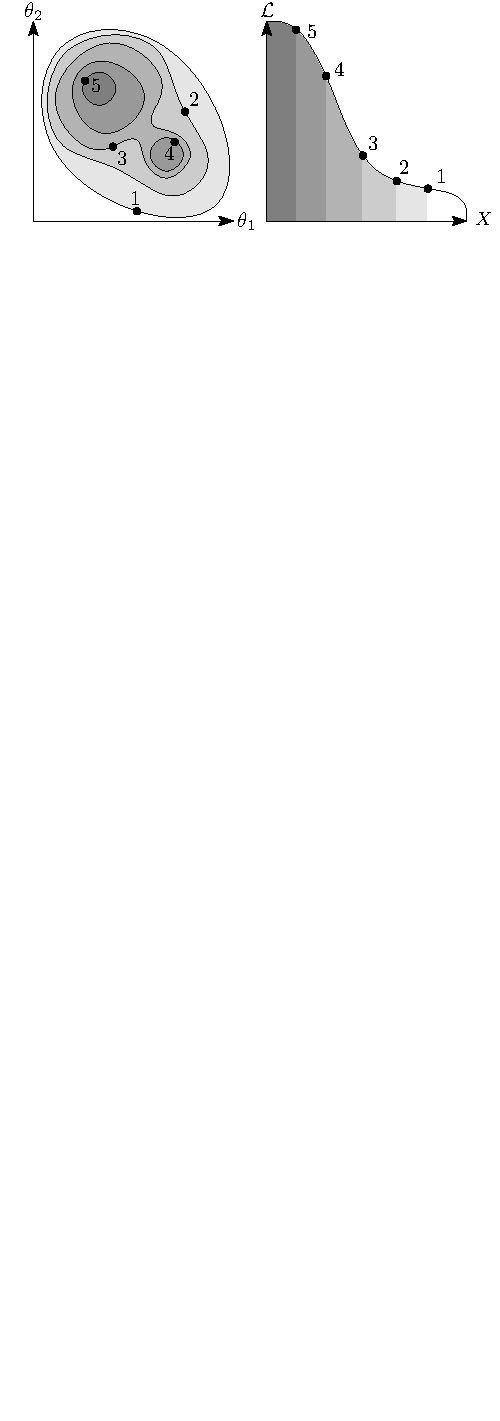
\includegraphics[width=\textwidth]{chapters/bayesian_inference/figures/contour_nested}
  \caption{%
    The nested sampling volume transformation.
    Left: five iso-likelihood contours of a two-dimensional multi-modal likelihood function \(\lik(\params)\). Each contour encloses some fraction of the prior \(X\), indicated by colour.
    Right: Likelihood \(\lik\) as a function of the volume \(X\) enclosed by the contour. The evidence is the area under this curve.\label{fig:bay:prior_volume}
  }
\end{figure}

An inverse derivation is to examine~\eqref{eqn:bay:ev_short}, and define a new integration variable \(\d{X} = \prior(\params)\:\d{\params}\). From this definition, the notion of prior volume~\eqref{eqn:bay:prior_volume} follows, which may be inverted to give \(\lik(X)\). Mathematically inclined readers may like to consider how this procedure is related to Lesbesque integration.

The beauty of this process is that it completely removes all complications such as geometry, topology and dimensionality, reducing~\eqref{eqn:bay:ev_X} to a one dimensional integral.  We may now evaluate the evidence using standard quadrature techniques:
\begin{equation}
  \ev \approx \sum_{i} w_i \lik(X_i),
  \label{eqn:bay:quadrature}
\end{equation}
where \(\{X_i\}\) are the quadrature points and \(\{w_i\}\) are the quadrature weights. 

\subsection{Computing the prior volumes}

This is all well and good, but so far all we have done is transfer the complications (geometry, topology and dimensionality) from the evidence integral~\eqref{eqn:bay:ev_short} to the integral which calculates the prior volume~\eqref{eqn:bay:prior_volume}. John's true genius is to come up with a scheme that allows one to {\em estimate\/} the prior volume \(X\) in a quantifiable way.

The method relies on having a sampling procedure capable of producing a sample \(\tilde{\params}\) distributed according to the prior \(\prior\), subject to the constraint that it lies within the likelihood contour \(C(\liks)\).  This is termed ``sampling within a hard-edged likelihood constraint''.  In theory shouldn't be any more challenging than traditional sampling techniques such as Metropolis-Hastings \citep{skilling2006}. 

Importantly, a sample within \(C(\liks)\) distributed according to the prior \(\prior\) will have its prior volume \(X\) drawn {\em uniformly\/} within \([0,X_\ast]\), \(X_\ast=X(\liks)\). This demonstrates another reason why the prior volume is a powerful variable to work with.

\subsection{Single-point nested sampling}

If one draws an initial sample from \(C(0)\) (i.e.\ the entire space) according to the prior \(\prior\), one will have generated a point with prior volume \(X_1\) and likelihood \(\lik_1\). On average, a single sample will cut the prior in two, and the mean \(\mean{X_1}=\frac{1}{2}\). At this value of \(X_1\), it is unlikely that the likelihood is large enough to contribute to the evidence integral (\(X_1\gg e^{-H}\)) so we should go deeper.

If one then generates \(X_2\) by sampling from the contour defined by the previous point \(C(\lik_1)\), then \(X_2=t_2\times X_1\), where \(t\) is a uniform variable drawn from \([0,1]\). We thus find that the on average the second sample will have a mean \(\mean{X_2} = \frac{1}{4}\). 

Repeating this process by using the previous contour as the hard likelihood constraint will mean that we sample within regions closer and closer to the peak, with \(\mean{X_i} = 2^{-i}\). When \(X_i\sim e^{-H}\), then the samples with these quadrature points start contributing to the evidence integral. Eventually, the samples compress too far (\(X_i\ll e^{-H}\)) and no longer contribute to the evidence, and the algorithm should stop.

More precisely, one finds that:
\begin{equation}
  X_i = \prod_{j=1}^i t_j,
  \label{eqn:bay:X_i}
\end{equation}
where each \(t_j\) is an independent random variable drawn uniformly from \([0,1]\). As \(i\) increases, \(X_i\) becomes distributed {\em log-normally\/} with:
\begin{align}
  \log X_i  &\approx -i \pm \sqrt{i},
  \label{eqn:bay:log_normal_1_1}
  \\
  P(X_i) &= \frac{1}{\sqrt{2\pi i} X}\exp\left[ -\frac{{\left( \log X_i - i \right)}^2}{2 i}  \right],
  \label{eqn:bay:log_normal_1_2}
\end{align}
This follows by taking logarithms of~\eqref{eqn:bay:X_i} and applying the central limit theorem. This is particularly impressive, since one finds that the samples compress the prior space {\em exponentially}. In general, the logarithmic compression from the prior to the posterior \(H\) tends to be linear in dimensionality \(d\), so single point nested sampling scales linearly with dimensionality.

As this scheme progresses, one is left with a set of likelihoods \(\lik_i\), each paired with a volume \(X_i\). These volumes are not deterministically known, but defined by the probabilistic definition~\eqref{eqn:bay:X_i}. The evidence may be approximated as:
\begin{equation}
  Z = \sum_{i=1}^n \lik_i \times (X_{i-1}-X_{i}),
  \label{eqn:bay:ev_sum}
\end{equation}
where for simplicity the quadrature weighting is taken as \(w_i = X_{i-1}-X_i\). This means that the evidence is also implicitly probabilistic. Instead of computing an exact evidence, one may infer the distribution of evidence values that it could take.

In general, single point nested sampling will not produce a particularly accurate evidence estimation, but we can go one better.


\subsection{Multi-point nested sampling}
Instead of working with a single sample, one could initially generate a set of \(\nlive\) ``live points'' distributed across the prior. The lowest likelihood point will have likelihood \(\lik_1\) and a volume \(X_1 = t\) where \(t\) is distributed as the largest of \(\nlive\) uniform samples in \([0,1]\). Elementary probability shows that:
\begin{equation}
  P(t) = \nlive t^{\nlive-1}.
  \label{eqn:bay:t_prob}
\end{equation}
If this point is deleted, and replaced with a new point drawn from the contour defined by \(\lik_1\), then one will still have \(\nlive\) points, now uniformly distributed uniformly in \([0,X_1]\). Proceeding onward, one finds that the volume becomes log-normally distributed:
\begin{align}
  \log X_i  &\approx -\frac{i}{\nlive} \pm \sqrt{\frac{i}{\nlive}}.
  \label{eqn:pc:X_full}
\end{align}
The prior space compression is slower than single point nested sampling, but with a correspondingly lower error. This therefore produces a more accurate inference on the evidence.

The deleted point is then added to a list of ``dead points'' which can then be used to make inferences on the evidence using equation~\eqref{eqn:bay:ev_sum}.


\subsection{Posterior inference}
Nested sampling is designed to calculate the evidence, but it also produces posterior samples as a by-product of the calculation. Samples can be obtained by sampling randomly under the posterior curve.% (Figure~\ref{fig:bay:posterior}). 
Since we have partitioned the area into regions of size \(\lik_i w_i\), we can use this as an importance weighting.

%\begin{figure}[tp]
%  \centering
%  \tikzsetnextfilename{posterior_plot}
%  \includegraphics[width=\textwidth]{chapters/bayesian_inference/plots/posterior.tikz}
%  \caption{%
%    Posterior samples.\label{fig:bay:posterior}
%}
%\end{figure}

Thus, dead points may be used as posterior samples with importance weighting:
\begin{equation}
  p_i = \frac{\lik_i w_i}{\ev},
  \label{eqn:bay:posterior_weight}
\end{equation}
where the additional factor of \(\ev\) merely ensures that they sum to \(1\) for consistency.



\subsection{Terminating the algorithm}
One does not wish to continue compressing the space once \(X_i\ll e^{-H}\) for two reasons. The first reason is that this will not give any further accuracy on the evidence calculation. The second is more important. The region beneath \(X_i\ll e^{-H}\) is not statistically relevant. Scientists used to maximum likelihood methods find this difficult to swallow, and often desire algorithms that will maximise the function to find the highest peak. In high dimensions, the absolute peak occupies such a vanishingly small percentage of the prior mass that it is totally irrelevant for the purposes of inference. In the case of a Gaussian likelihood, the peak value is a useful {\em summary statistic\/} but nothing more than that. Otherwise, one should not concern oneself with maximum likelihood, only in an accurate description of the peak provided by a set of samples.

%
\begin{figure}[tp]
  \centering
  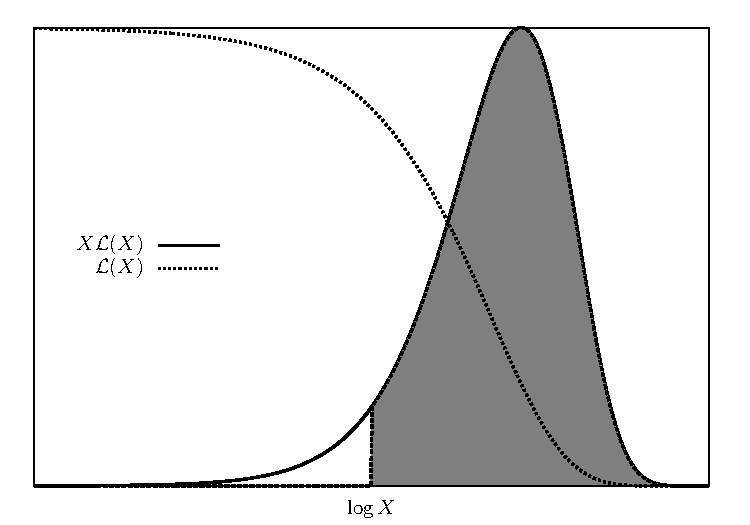
\includegraphics[width=\columnwidth]{chapters/bayesian_inference/figures/gaussian_weight}
  \caption{%
    Plot of a generic likelihood as a function of the prior volume \(\lik(X)\). In high dimensions, the likelihood is only visible if plotted against \(\log X\) (dashed curve). However, the evidence is better visualised by plotting \(X\log(X)\) (solid curve). The area under the solid curve corresponds to the evidence. The magnitude of the solid curve is proportional to the importance weighting. Nested sampling proceeds from high to low volumes. After some time, the live points no longer contribute significantly to the evidence, and the algorithm terminates at this point.\label{fig:bay:gaussian_weight}
  }
\end{figure}
%
As nested sampling proceeds, the likelihoods \(\lik_i\) monotonically increase, but the weights \(w_i\) monotonically decrease. This results in a peak in importance weights~\eqref{eqn:bay:posterior_weight} that can be seen in Figure~\ref{fig:bay:gaussian_weight}. We terminate the algorithm once the remaining posterior mass (white region) left in the live points is some small fraction of the currently calculated evidence (dark region). The posterior mass left in the live points at iteration \(i\) can be estimated by:
\begin{equation}
  \ev_\slive \approx \mean{\lik}_\slive X_i,
  \label{eqn:bay:live_evidence}
\end{equation}
where the average is taken over the live points. Since this is typically an underestimate at early times, this will not cause premature termination.



\subsection{Nested sampling: summary}
\label{sec:bay:comp_space}
\begin{itemize}
  \item The algorithm initialises by sampling \(\nlive\) points from the prior distribution \(\prior(\params)\). 
  \item At iteration \(i\), the point with the lowest likelihood \(\lik_i\) is deleted, and then replaced by a new point, which is drawn from the prior subject to the constraint that its likelihood is greater than \(\lik_i\). 
  \item The evidence may be inferred from the dead points via:
    \begin{align}
      \ev &= \sum_{i=1}^n w_i \lik_i, &
      X_i &= \prod_{j=1}^{i} t_j, \nonumber \\
      w_i &= X_{i-1}-X_{i},  & 
      t_j &\sim U[0,1].\nonumber 
    \end{align}
  \item The algorithm terminates when:
    \begin{equation}
      X_i \times \mean{\lik}_\slive \ll \ev.
    \end{equation}
  \item A set of posterior samples may be produced using the dead points with importance weighting:
    \begin{equation}
      p_i = \frac{w_i\lik_i}{\ev}.\nonumber
    \end{equation}

\end{itemize}


\section{Conclusion}
The following two chapters are concerned with describing my contributions to nested sampling theory and implementation in the algorithm \PolyChord{}. After that I describe a novel numerical approach to solving differential equations which is relevant for my work in the field of quantum cosmology.

\begin{subappendices}
  \section{Traditional sampling methods}
\label{chp:sm}
\subsection{Inverse transform sampling}
\label{sec:sm:inverse_transform}

In the one-dimensional case, this amounts to converting a uniform random variable (which are easy to generate) into a variable sampled from a general distribution \(f(\theta)\). One first finds its cumulative distribution function (CDF):
\begin{equation}
  F(\theta) = \int\limits_{-\infty}^\theta f(\theta^\prime) \d{\theta^\prime},
\end{equation}
computes the inverse of the CDF, and then applies this function to a uniform random variable  \(x\sim U(0,1)\) to generate a variable \(\theta = F^{-1}(x)\), which is distributed according to \(f(\theta)\). 

In the general \(D\)-dimensional case, one calculates \(D\) conditional distributions \(\{f_i:i=1\ldots,D\}\): by marginalising over parameters with indices greater than \(i\) and conditioning on parameters with indices less than \(i\):
%
\begin{equation}
  f_i(\theta_i|\theta_{i-1},\ldots,\theta_1) 
  =
  \frac{%
    \int f_i(\params) d\theta_{i+1}\ldots \d{\theta_{N}}
  }{%
    \int f_i(\params) d\theta_{i}\ldots \d{\theta_{N}}
  },
\end{equation}
%
Integrating these yields \(D\) conditional CDFs:
%
\begin{equation}
  x_i = F_i(\theta_i|\theta_{i-1},\ldots,\theta_1) = \int\limits_0^{\theta_i} f_i(\theta_i^\prime|\theta_{i-1},\ldots,\theta_1) \d{\theta_i^\prime}.
\end{equation}
%
Inverting this gives \(\theta_i = F^{-1}_i(x_i|\theta_{i-1},\ldots,\theta_1)\), which constitutes a set of relations sequentially transforming \(D\) uniform random variables \(\{x_i\}\) into \(\{\theta_i\}\) distributed according to \(f(\params)\).

In many cases, the prior \(\prior(\params)\) is separable, and the above equations are easily calculated. For sections of the parameters which are not separable, the calculation can become more involved. We include a few demonstrations of this procedure in Section~\ref{sec:pc:prior_transformations}. In the language of nested sampling the \(D\) uniform random variables \(x_i\) are termed elements of the ``unit hypercube'' and \(\theta_i\) are elements of the ``physical space''.

\subsection{Prior transformations}
\label{sec:pc:prior_transformations}
Here we give examples of the procedure for calculating the transformation from the unit hypercube to the physical space. We demonstrate it for a separable case, and a more complicated dependent case

To recap, we aim to compute the inverse of the functions \(F_i\): 
\begin{equation}
  F_i(\theta_i|\theta_{i-1},\ldots,\theta_0) = \int\limits_0^{\theta_i} \pi_i(\theta_i^\prime|\theta_{i-1},\ldots,\theta_1) \d{\theta_i^\prime},
  \label{eqn:pc:appFi}
\end{equation}
%
where:
%
\begin{equation}
  \pi_i(\theta_i|\theta_{i-1},\ldots,\theta_0) 
  =
  \frac{%
    \int \pi_i(\params) d\theta_{i+1}\ldots d\theta_{N}
  }{%
    \int \pi_i(\params) d\theta_{i}\ldots d\theta_{N}
  }.
  \label{eqn:pc:apppii}
\end{equation}
\(\bFF\) maps from \(\params\) in the physical space onto the unit hypercube injectively. 



\subsubsection{Separable priors}
\label{sec:pc:separable_priors}
A separable prior satisfies:
\begin{equation}
  \pi(\params) = \prod_i\pi_i(\theta_i).
  \label{eqn:pc:separability}
\end{equation}
This has the fortunate side effect that the functions \(F_i\) only depend on \(\theta_i\):
\begin{equation}
  F_i(\theta_i|\theta_{i-1},\ldots,\theta_0) = F_i(\theta_i).
\end{equation}

Solving a separable prior thus amounts to solving a one-dimensional inverse-transform sampling problem. We demonstrate this procedure for two cases, a rectangular uniform prior, and a Gaussian prior.

\subsubsection{Uniform prior}
\label{sec:pc:uniform_prior}
%------------ commands for this section --------------
\newcommand{\thetamin}{\theta_\smin} % Minimum uniform prior
\newcommand{\thetamax}{\theta_\smax} % Maximum uniform prior
%-----------------------------------------------------
A rectangular uniform prior is defined by two parameters, \({\thetamin,\thetamax}\):
\begin{equation}
  \pi(\theta) = 
  \left\{
    \begin{array}{rl}
      {(\thetamax - \thetamin)}^{-1} 
      &
      \text{for }\thetamax<\theta_i<\thetamin \\
      0 & \text{otherwise.}
    \end{array}
  \right.
\label{eqn:pc:uniform_prior}
\end{equation}

Computing \(F(\theta)\) we find:
\begin{align}
  F(\theta) &= \int_{-\infty}^\theta \pi(\theta^\prime)\d{\theta^\prime}, \nonumber\\
  &= \frac{\theta-\thetamin}{\thetamax-\thetamin},
  \label{eqn:pc:calc_uniform_trans}
\end{align}
with \(F=0\) or \(1\) either side of \(\thetamin\) and \(\thetamax\) respectively. Inverting the equation \(F(\theta)=x\) we find:
\begin{equation}
  \theta = \thetamin+(\thetamax-\thetamin)x,
  \label{eqn:pc:uniform_trans}                           
\end{equation}
is the transformation from \(x\) in the unit hypercube to \(\theta\) in the physical space.

\subsubsection{Gaussian prior}
\label{sec:pc:gaussian_prior}
Defining a Gaussian prior with mean \(\mu\) and standard deviation \(\sigma\):
\begin{equation}
  \pi(\theta) = \frac{1}{\sqrt{2\pi}\sigma}\exp{\left[-\frac{{(x-\mu)}^2}{2\sigma^2}\right]},
  \label{eqn:pc:gaussian_prior}
\end{equation}
We find that the procedure above yields:
\begin{equation}
  \theta = \mu + \sqrt{2}\sigma\text{erfinv}(2x-1),
  \label{eqn:pc:gaussian_trans}                           
\end{equation}
where \(\text{erfinv}\) is the conventional inverse error function.




\subsubsection{Forced identifiability priors}
\label{sec:pc:forced_identifiablility}

As an example of a prior that is not separable in the parameters, we consider a forced identifiability prior. Here, \(n\) parameters are distributed uniformly between \(\thetamin\) and \(\thetamax\), but subject to the constraint that they are ordered numerically. This is a particularly useful prior in the reconstruction of functions using a spline with movable knots \citep{vazquez_knots,knottedsky1,knottedsky2,planck2015-a24}. In this case, the  horizontal locations of the knots must be ordered.

The required prior is uniform in the hyper-triangle defined by \(\thetamin<\theta_1<\cdots<\theta_n<\thetamax\), and zero everywhere else:
%
\begin{equation}
  \pi(\params) = 
  \left\{
    \begin{array}{rl}
      \frac{1}{n!{(\thetamax - \thetamin)}^{n}} 
      &
      \text{for }\thetamin<\theta_1<\cdots<\theta_n<\thetamax \\
      0 &\text{otherwise.}
    \end{array}
    \right.
\label{eqn:pc:sorted_uniform_prior}
\end{equation}

To calculate equations~\eqref{eqn:pc:appFi} \&~\ref{eqn:pc:apppii} we integrate over the constant distribution, taking care with the limits. We find:
\begin{align}
  \pi_i(\theta_i|\theta_{i-1},\ldots,\theta_0) &= \frac{(n-i+1){(\theta_i-\theta_{i-1})}^{n-i}}{{(\thetamax-\thetamin)}^{n-i+1}},\\
  F_i(\theta_i|\theta_{i-1},\ldots,\theta_0) &= {\left(\frac{\theta_i-\theta_{i-1}}{\thetamax-\theta_{i-1}}\right)}^{n-i+1},
  \label{eqn:pc:sorted_uniform_calc}
\end{align}
where for consistency we define \(\theta_0 = \thetamin\). Hence solving \(x_i=F(\theta_i|\theta_{i-1},\ldots,\theta_0)\) for \(\theta_i\) we find:
\begin{equation}
  \theta_i = \theta_{i-1}+ (\thetamax-\theta_{i-1})x_i^{1/(n-i+1)}.
  \label{eqn:pc:sorted_uniform_trans}
\end{equation}
This enables \(\{\theta_i\}\) to be calculated sequentially from \(\{x_i\}\). We may interpret this transformation as \(\theta_i\) being distributed as the smallest of \(n-i+1\) uniformly distributed variables in the range \([\theta_{i-1},\thetamax]\).



\subsection{Rejection sampling}
\label{sec:sm:rejection}

The principle behind rejection sampling is simple, and best demonstrated graphically as in Figure~\ref{fig:sm:rej}. If one requires some samples from a complicated distribution \(f(x)\), but has the knowledge that it satisfies \(f(x)<g(x)\) for some simpler distribution \(g(x)\), then one may sample from \(g\), and accept only those samples with probability less than \(f\). 

\begin{figure}[tp]
  \tikzsetnextfilename{rejection}
  \centering
  \includegraphics[width=\textwidth]{appendices/sampling_methods/plots/rejection.tikz}
  \caption{Rejection sampling. One may produce samples from some complicated distribution \(f(x)\) using a simpler distribution \(g(x)\) provided that \(g(x)>f(x)\) within the domain of interest. One samples from \(g\), and accepts only those samples that lie under the \(f\) curve.}\label{fig:sm:rej}
\end{figure}

Obviously this will be very inefficient unless \(g(x)\) happens to be rather close to \(f(x)\). One finds that in general this inefficiency is exaggerated by the curse of dimensionality.

\subsection{Metropolis---Hastings}
\label{sec:sm:mh}
Metropolis---Hastings approaches are an extremely widely used methodology for generating a sequence of samples (or points) from some posterior \(\posterior(x)\).

A sequence of \(T\) points is termed a {\em chain\/} \(\chain_T\):
\begin{equation}
  \chain_T = \{ x^{(t)}: t=1\cdots T \}.
\end{equation}
A new point \(x^{(t+1)}\) is generated from a proposal density \(\proposal\) which depends on the current state \(x^{(t)}\). Typically \(\proposal(x|x^{(t)})\) might be a Gaussian distribution centered on the current value of \(x^{(t)}\):
\begin{equation}
  \log \proposal(x|x^{(t)}) = \text{const} -\frac{{\left[ x-x^{(t)} \right]}^2}{2\varepsilon^2},
\end{equation}
but in general the proposal density can be any fixed density from which we may draw samples easily.

A new state \(x\) is proposed from the proposal density \(\proposal(x|x^{(t)})\), and it is accepted with probability:
\begin{equation}
  p_\mathrm{accept}(x|x^{(t)}) = \frac{\posterior(x)}{\posterior(x^{(t)})}\frac{\proposal(x^{(t)}|x)}{\proposal(x|x^{(t)})}.
\end{equation}
If the step is accepted, then \(x^{(t+1)}=x\), otherwise \(x^{(t+1)} = x^{(t)}\). This procedure can be seen schematically in Figure~\ref{fig:sm:MH}.
\begin{figure}[tp]
  \centering
  \tikzsetnextfilename{MH}
  \includegraphics[width=\textwidth]{appendices/sampling_methods/plots/MH.tikz}
  \caption{Metropolis-Hastings. Here we have some degenerate two-dimensional posterior \(\posterior\), and a circular proposal distribution \(\proposal\).}\label{fig:sm:MH}
\end{figure}


This has the distinct advantage that it does not require one to take into account the overall normalisation of the posterior, circumnavigating any issues associated with computing the evidence \(\ev\), since:
\begin{equation}
  \frac{\posterior(x)}{\posterior(x^{(t)})} \equiv
  \frac{\lik(x)\prior(x)}{\lik(x^{(t)})\prior(x^{(t)})}.
\end{equation}
It is important to note that the chain \(C_T\) will comprise \(T\) samples which are {\em correlated}. If the proposal distribution amounts to a random walk with step size \(\varepsilon<\sigma_{\min{}}\), and the longest lengthscale in the probably region is \(\sigma_{\max{}}\)  then one will expect: \(\tau \sim {(L/\varepsilon)}^2\). If \(\varepsilon>\sigma_{\min{}}\), then one starts to expect a very low acceptance rate, so typically for a isotropic random walk, the timescale on which one expects to generate independent samples is:
\begin{equation}
  \tau \sim \left( \frac{\sigma_{\max{}}}{\sigma_{\min{}}} \right).
\end{equation}
In theory, given that the above relation has no dimensionality attached to it, Metropolis Hastings can be extremely successful in high dimensions. However, there are several issues.

First, one does not initially a-priori have a good starting point. There is therefore a period of ``burn-in'' attached to MH methods. Knowing when this period is truely over, and one is starting to generate random samples can be challenging in the general case.

In many cases, \(\tau\gg1\) resulting in unacceptable run-times. This can be ameliorated by choosing a proposal distribution \(\proposal\) that better agrees with the posterior \(\posterior\). However, this amounts to adding in many effective tuning parameters. Many algorithms work by having a ``learning'' phase, whereby the algorithm deduces for itself a good correlated Gaussian proposal distribution, but given the fact that this is not strictly Markovian care must be taken.



\subsection{Slice sampling}
\label{sec:sm:slice}
Radford Neal initially proposed slice sampling as an effective methodology for generating samples numerically from a given posterior \(\posterior(\params)\). One first chooses a `slice' (or probability level) \(\posterior_0\) uniformly within \([0,\posterior_\smax]\). One then samples uniformly within the \(\params\)-region defined by \(\posterior(\params)>\posterior_0\). The similarity with the iso-likelihood contour sampling required by nested sampling should be clear. In the one-dimensional case, he suggests the sampling procedure detailed in Figure~\ref{fig:bay:1d_slice}.

\begin{figure}[tp]
  \centerline{%
    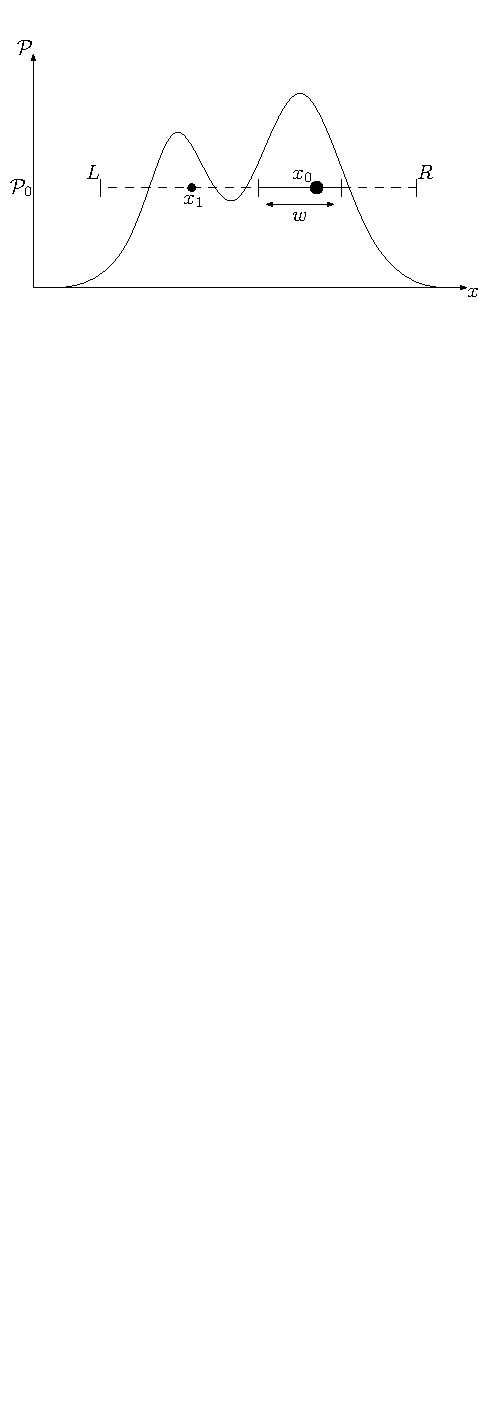
\includegraphics[width=\textwidth]{appendices/sampling_methods/figures/slice}
  }

  \caption{Slice sampling in one dimension. 
    Given a probability level (or slice) \(\posterior_0\), slice sampling samples within the horizontal region defined by \(\posterior>\posterior_0\). 
    From an initial point \(x_0\) within the slice (\(\posterior(x_0)>\posterior_0\)), a new point \(x_1\) is generated within the slice with a distribution \(P(x_1|x_0)\).
    External bounds are first set on the slice \(\hat{L}<x_0<\hat{R}\) by uniformly expanding a random initial bound of width \(w\) until they lie outside the slice (Neal terms this the {\em stepping out\/} procedure). 
    \(x_1\) is then sampled uniformly within these bounds.  
    If \(x_1\) is not in the slice, then \(\hat{L}\) or \(\hat{R}\) is replaced with \(x_1\), ensuring that \(x_0\) is still within the slice.
    This procedure is guaranteed to generate a new point \(x_1\), and satisfies detailed balance \(P(x_0|x_1) = P(x_1|x_0)\). Thus, if \(x_0\) is drawn from a uniform distribution within the slice, so is \(x_1\).\label{fig:bay:1d_slice}
  }
\end{figure}

In higher dimensions,~\cite{NealSlice} suggests a variety of MCMC-like methods. The simplest of these is implemented by sampling each of the parameter directions in turn. Since each one-dimensional slice requires \(\bigO{\text{a few}}\) likelihood calculations, the number of likelihood calculations required scales linearly with dimensionality, providing the region is efficiently navigated. 

Multi-dimensional slice sampling has many of the benefits of a traditional MH approach, and uses a proposal distribution which is much more efficient at sampling a hard likelihood constraint. This makes is a very suitable candidate for use within a nested sampling algorithm \citep{skilling2006}. 

Problems may occur with slice sampling if the peaks in Figure~\ref{fig:bay:1d_slice} are separated by a large distance. In this case it is still theoretically true that procedure satisfies detailed balance, and thus the algorithm will eventually jump one from one peak to the other. Practically however, this could take many Hubble times, and to all intents and purposes the distribution is not explored correctly. It is worth noting that \PolyChord{} (Chapter~\ref{chp:pc}) circumvents this difficulty by explicitly evolving posterior modes separately.



\subsection{Thermodynamic integration}
The traditional method of computing the evidence from MCMC procedures is via {\em thermodynamic integration}.
The aim is to compute:
\begin{equation}
  \ev = \int \lik(\Theta) \prior(\Theta) \d{\Theta}.
\end{equation}
Inspired by thermodynamics, we define the posterior \(\posterior_\beta \propto \lik^\beta\prior\) at temperature \(\beta\) as:
\begin{align}
  \posterior_\beta(\Theta) &= \frac{\lik^{\beta}(\Theta) \prior(\Theta)}{\ev_\beta}, 
  \label{eqn:bay:posteriorb}
  \\
  \ev_\beta &= \int\lik^{\beta}(\Theta) \prior(\Theta) \d{\Theta}.
  \label{eqn:bay:evb}
\end{align}
If the likelihood is interpreted as a Boltzmann-like probability distribution, then:
\begin{equation}
{\lik(\Theta)}^\beta = \exp[-\beta E(\Theta)],
\end{equation}
is the Boltzmann probability of finding a system with inverse temperature \(\beta = T^{-1}\) in state \(\Theta\) with energy \(E\), and the partition function is \(\ev_\beta\).

Inspired by thermodynamics, one can see that:
\begin{equation}
  \frac{\d{}}{\d{\beta}}\log\ev_\beta = \frac{\int  \lik^\beta \prior \log\lik\d{\Theta}}{\int\lik\prior \d{\Theta}} = \int \posterior_\beta \log\lik\d{\Theta} =  \mean{\log\lik}_\beta.
  \label{eqn:bay:thermo}
\end{equation}
Hence, integrating the above equation yields:
\begin{equation}
  \log\ev_1-\log\ev_0 = \log\ev = \int_{0}^{1}\mean{\log\lik}_\beta.
  \label{eqn:sm:thermo}
\end{equation}
The key point is that we may compute the mean \(\mean{\log\lik}_\beta\) from a set of samples from the posterior \(\posterior_\beta\). If we therefore generate a set of samples for a range of temperatures \(\beta\), the one-dimensional integral above may be computed easily. Thermodynamic calculation of the evidence therefore is equivalent to running multiple MCMC runs at several temperatures.
This however suffers from the disadvantage that it is difficult to produce an estimate of the error in computing~\eqref{eqn:sm:thermo}. 


\end{subappendices}



%
% Extending nested sampling
% -------------------------
%
\chapter{Extending Nested Sampling}
\label{chap:ens}

\section{Evidence estimates and errors}                            
\label{sec:ens:evidences}

\cite{skilling2006} initially advocated using Monte-Carlo methods to estimate the evidence error, although this requires the storage of the entire chain of dead points, rather than just the subset usually stored for posterior inferences. For high-dimensional problems, the number of dead points is prohibitively large, and cannot be stored.

\cite{MultiNest2} use an alternative method based on the relative entropy (also suggested by~\cite{skilling2006}). 

\cite{Keeton} suggests a more intuitive methodology of estimating the error, and it is this which we use, although it must be heavily adapted for the case of variable numbers of live points and clustering.

\subsection{Basic theory}
\label{sec:ens:basic_theory}

We wish to compute the sum:
%
\begin{equation}
  \ev = \sum\limits_{i} (X_{i-1}-X_{i})\lik_i.
  \label{eqn:ens:app_ev}
\end{equation}
%
However, we do not know the volumes \(X_i\) exactly, so we can only make inferences about \(\ev\), in terms of a probability distribution \(\Prob{\ev}\). In practice, all we need to compute is the mean and variance of this distribution:
\begin{align}
  \text{mean}(\ev) &\equiv \overline{\ev},\\
  \text{var}(\ev) &\equiv \overline{\ev^2}-\overline{\ev}^2.
\end{align}
%
At iteration \(i\), the \(\nlive\) live points are each uniformly sampled within a contour of volume \(X_{i-1}\). The volume \(X_i\) will be the largest volume out of \(\nlive\) uniform volume samples in volume \(X_i\).
Thus \(X_i\) satisfies the recursion relation:
%
\begin{align}
  X_i &= t X_{i-1}, \qquad X_0=1, \label{eqn:ens:rr_x} \\
  P(t) &= \nlive t^{\nlive - 1}, \label{eqn:ens:Pt}
\end{align}
%
where the \(t\) and \(X_{i-1}\) are independent.

It is worth noting that the procedure described below will generate the mean and variance of the distribution, but in fact this is not quite what we want. The evidence is in practice approximately log-normally distributed. Thus, it is better to report the mean and variance of \(\log\ev\), defined by:
\begin{align}
  \text{mean}(\log\ev) &= 2\log\overline{\ev} - \frac{1}{2}\log\overline{\ev^2},\\
  \text{var}(\log\ev) &= \log\overline{\ev^2}-2\log\overline{\ev}.
\end{align}


\subsection{Computing the mean evidence}
\label{sec:ens:basic_mean}

While it is possible to take equations~\eqref{eqn:ens:app_ev},\ref{eqn:ens:rr_x} \&~\ref{eqn:ens:Pt} and compute the mean as a general formula~\citep{Keeton}, in the case of clustering this is uninformative. 
In fact, for large-dimensional spaces using the full formula would require storage of a prohibitively large amount of data. The calculation is better accomplished by a set of recursion relations, which update the mean evidence and its error at each step. 

For now, assume that we have \(n\) live points currently enclosed by some likelihood contour \(\lik\) of volume \(X\), and \(\ev\) is the last value of the evidence calculated from all of the points that have died so far. By considering~\eqref{eqn:ens:app_ev},\ref{eqn:ens:rr_x}\&\ref{eqn:ens:Pt}, when we kill off the outermost point, we may adjust the values of \(\ev\) and \(X\) using:
%
\begin{align}                                                         
\ev &\to \ev + (1-t)X\lik,
\label{eqn:ens:rr_Z}
\\
X &\to tX.
\label{eqn:ens:rr_X}
\end{align}
%
Taking the mean of these relations, we may use the facts that \(t\) and \(X\) are independent random variables and that \(P(t) = n t^{n-1}\), to find the recursion relations:
\begin{align}
  \overline{\ev} &\to \overline{\ev} + \frac{1}{n+1}\overline{X}\lik,
  \label{eqn:ens:rr_Zb}
  \\
  \overline{X} &\to \frac{n}{n+1}\overline{X}.
  \label{eqn:ens:rr_Xb}
\end{align}
%

\subsection{Computing the evidence error}
\label{sec:ens:basic_error}
To estimate \(\overline{\ev^2}\), we square~\eqref{eqn:ens:rr_Z} and~\eqref{eqn:ens:rr_X} and multiply both together to obtain:
%
\begin{align}
  \ev^2 &\to \ev^2 + 2(1-t)\ev X\lik +  {(1-t)}^2X^2\lik ^2,
  \label{eqn:ens:rr_Z2b}
  \\
  \ev X &\to t\ev X + t(1-t)X^2\lik,
  \label{eqn:ens:rr_ZXb}
  \\
  X^2 &\to t^2X^2.
  \label{eqn:ens:rr_X2b}
\end{align}
%
Note that we now need to keep track of the variable \(\ev X\), as these two are not independent.
Taking the averages of the above yields:
\begin{align}
  \overline{\ev^2} &\to \overline{\ev^2} + \frac{2\overline{\ev X}\lik}{n+1} +  \frac{2\overline{X^2}\lik^2}{(n+1)(n+2)},
  \\
  \overline{\ev X} &\to \frac{n\overline{\ev X}}{n+1} + \frac{n\overline{X^2}\lik}{(n+1)(n+2)},
  \\
  \overline{X^2} &\to \frac{n}{n+2}\overline{X^2}.
\end{align}

\subsection{The full calculation}
\label{sec:ens:basic_full}

There are therefore five quantities to keep track of: 
\[ \overline{\ev},\quad\overline{\ev^2},\quad\overline{\ev X},\quad \overline{X},\quad\overline{X^2}.\]
These should be initialised at \(\{0,0,0,1,1\}\) respectively, and updated using equations~\eqref{eqn:ens:rr_Zb},\ref{eqn:ens:rr_Z2b},\ref{eqn:ens:rr_ZXb},\ref{eqn:ens:rr_Xb},\ref{eqn:ens:rr_X2b} in that order. In fact, we keep track of the logarithm of these quantities, in order to avoid machine precision errors.





\section{Evidence estimates and errors in clusters}
\label{sec:ens:evidences_clusters}
This analysis follows that of Section~\ref{sec:ens:evidences}. We recommend that you have understood the methods described there before continuing.


Throughout the algorithm, there will in general be \(m\) identified clusters. In doing so, we wish to keep track of the volume of each cluster \(\{X_1,\ldots,X_m\}\), the global evidence and its error \(\ev,\ev^2\) and the local evidences and their errors \(\{\ev_1,\ev_1^2\ldots,\ev_m,\ev_m^2\}\). At each iteration, the point with the lowest likelihood \(\lik\) will be killed from cluster \(p\), \({(1\le p\le m)}\). 


\subsection{Evidence}
\label{sec:ens:cluster_ev}

We thus need to update the global evidence, the local evidence of cluster \(p\), and the volume of cluster \(p\):
%
\begin{align}
  \ev &\to \ev + (1-t)X_p\lik,
  \label{eqn:ens:rr_ev}\\
  \ev_p &\to \ev_p + (1-t)X_p\lik,
  \label{eqn:ens:rr_evi}\\
  X_p &\to t X_p.
  \label{eqn:ens:rr_Xi}
\end{align}
%
Since \(t\) will be distributed with \(P(t) = n_p t^{n_p-1}\),
taking the mean of these yields:
%
\begin{align}
  \overline\ev &\to \overline\ev + \frac{\overline X_p \lik}{n_p+1},\\
  \overline\ev_p &\to \overline\ev_p + \frac{\overline X_p \lik}{n_p+1},\\
  \overline X_p &\to \frac{n_p\overline X_p }{n_p+1}. 
\end{align}
%
Keeping track of \(\{\overline{\ev},\overline{\ev_p},\overline{X_p},p=1\ldots m\}\) and updating them using the recursion relations in the order above will produce a consistent evidence estimate for both the local and global evidence errors.


\subsection{Evidence errors}
\label{sec:ens:cluster_err}

We must also keep track of the local and global evidence errors. Taking the square of equations~\eqref{eqn:ens:rr_ev} \&~\ref{eqn:ens:rr_evi} yields:
%
\begin{align}
  \ev^2 &\to \ev^2 + 2 (1-t) \ev X_p \lik +  {(1-t)}^2 X_p^2 \lik^2, \\
  \ev_p^2 &\to \ev_p^2 + 2 (1-t) \ev_p X_p \lik +  {(1-t)}^2 X_p^2 \lik^2.
\end{align}
%
We can see that we're going to need to keep track of \(\{\overline{\ev X_p}, \overline{\ev_p X_p}, \overline{X_p^2}\}\) in addition to \(\{ \overline{\ev^2}, \overline{\ev_p^2} \}\). Taking various multiplications of equations~\eqref{eqn:ens:rr_ev},~\ref{eqn:ens:rr_evi} \&~\ref{eqn:ens:rr_Xi} finds:
%
\begin{align}
  \ev X_p   &\to t \ev X_p + (1-t)t X_p^2 \lik, \\
  \ev X_q   &\to   \ev X_q + (1-t) X_p X_q \lik \qquad (p\ne q),   \\
  \ev_p X_p &\to t \ev_p X_p + (1-t)t X_p^2 \lik, \\
  X_p^2     &\to t^2 X_p^2, \\
  X_p X_q   &\to t   X_p X_q.
\end{align}
%
Taking the mean of the above yields the recursion relations:
\begin{align}
  \overline{\ev^2} &\to \overline{\ev^2} + \frac{2\overline{\ev X_p}\lik_p}{n_p+1}  + \frac{2\overline{X_p^2}\lik^2}{(n_p+1)(n_p+2)}, \\
  \overline{\ev_p^2} &\to \overline{\ev_p^2} + \frac{2\overline{\ev_p X_p}\lik}{n_p+1}  + \frac{2\overline{X_p^2}\lik^2}{(n_p+1)(n_p+2)}, \\
  \overline{\ev X_p} &\to \frac{n_p\overline{\ev X_p}}{n_p+1}  + \frac{n_p\overline{X_p^2} \lik}{(n_p+1)(n_p+2)},   \\
  \overline{\ev X_q} &\to \overline{\ev X_p}  + \frac{\overline{X_p X_q} \lik}{(n_p+1)} \qquad (q\ne p),  \\
  \overline{\ev_p X_p} &\to \frac{n_p\overline{\ev_p X_p}}{n_p+1}  + \frac{n_p\overline{X_p^2} \lik}{(n_p+1)(n_p+2)},   \\
  \overline{X_p^2} &\to \frac{n_p\overline{X_p^2}}{n_p+2}, \\
  \overline{X_p X_q} &\to \frac{n_p\overline{X_p X_q}}{n_p+1}.
\end{align}
Keeping track of 
\[\{\overline{\ev^2},\overline{\ev_p^2},\overline{\ev X_p},\overline{\ev_p X_p},\overline{X_p^2},\overline{X_p X_q},p,q=1\ldots m\},\]
and updating them using the recursion relations in the order above will produce a consistent estimate for the local and global evidence errors.



\subsection{Cluster initialisation}
\label{sec:ens:cluster_init}
All that remains is to initialise the clusters correctly at the point of creation.

The starting initialisation of the evidence and volume is reasonable, there will be only a single cluster with volume \(1\), and all evidence related terms \(0\). At some point (possibly at the beginning, depending on the prior), the live points will split into distinct clusters, and the local volumes and evidences will need to be re-initialised.

At the point of splitting a cluster into sub-clusters, we partition the \(n\) live points into a \(N\) new clusters, with \(\{n_1,\ldots,n_N\}\) live points in each. If the volume of the splitting cluster is \(X_p\) initially, we need to know how to partition this volume into \(\{X_1,\ldots,X_N\}\). If the points are drawn uniformly from the volume, then the \(n_i\) will depend on the volumes via a multinomial probability distribution:
%
\begin{equation}
  P(\{n_i\}|X_p,\{X_i\}) \propto {X_1}^{n_1} \ldots X_N^{n_N}.
\end{equation}
%
We however want to know the probability distributions of the \(\{X_i\}\), given the \(\{n_i\}\). We can invert the above with Bayes' theorem, using an (improper) logarithmic prior on the volumes subject to the constraint that they sum to \(X_p\):
%
\begin{equation}
  P(\{X_i\}|X_p) \propto \frac{\delta(X_1+\cdots+X_N-X_p)}{X_1\cdots X_N}.
\end{equation}
%
Doing this shows the posterior \(P(\{X_i\}|X_p,\{n_i\})\) is a Dirichlet distribution with parameters \(\{n_i\}\). More importantly, we can use this to compute the means and correlations for the volumes \(\{X_i\}\):
%
\begin{align}
  \overline{X_i}&=  \frac{n_i}{n} \overline X_p, \\
  \overline{X_i^2}&= \frac{n_i(n_i+1)}{n(n+1)} \overline{X_p^2}, \\
  \overline{X_i X_j} &= \frac{n_i n_j}{n(n+1)} \overline{X_p^2}, \\
  \overline{X_i Y} &= \frac{n_i}{n} \overline{X_p Y} \qquad Y\in \{Z,Z_p,X_q\}.
\end{align}
%
The first equation recovers the intuitive result that the volume should split as the fraction of live points. Note, however that this requires a logarithmic prior. The third shows us that since \(\overline{X_i X_j}\ne\overline{X_i}\:\overline{X_j}\), the volumes are correlated at the splitting. This is to be expected.

We also need to initialise the local evidences and their errors. A consistent approach is to assume that the evidences also split in proportion to the cluster distribution of live points. Following the same reasoning as above, we find that:
\begin{align}
  \overline{Z_i}&=  \frac{n_i}{n} \overline Z_p \\
  \overline{Z_i X_i}&= \frac{n_i(n_i+1)}{n(n+1)} \overline{Z_p X_p} \\
  \overline{Z_i^2}  &= \frac{n_i(n_i+1)}{n(n+1)} \overline{Z_p^2} \\
\end{align}

Thus, at cluster splitting, all of the new local evidences, volumes and cross correlations are initialised according to the above.

This completes the mechanism for keeping track of the local and global evidences, their errors, and the local cluster volumes.


\section{Further generalisations}

It's worth noting that the procedures in the previous sections are amenable to a great many generalisations. We give a few examples in order to demonstrate this

First, if one desires a higher order of accuracy, one may update the rather simple quadrature in equation~\eqref{eqn:ens:app_ev} to:
\begin{equation}
  \ev = \sum\limits_{i} (X_{i-1}-X_{i}) \times \frac{1}{2}(\lik_i+\lik_{i-1}).
  \label{eqn:ens:app_trap_ev}
\end{equation}
In this case, the approach is identical to the method described above, one merely replaces the likelihood value with that of the average value of the last two likelihoods \((\lik_i + \lik_{i-1})/2\).
It is better to phrase the trapezoidal rule as in equation~\eqref{eqn:ens:app_trap_ev} as oppose to the more traditionally cited:
\begin{equation}
  \ev = \sum\limits_{i} \frac{1}{2}(X_{i-1}-X_{i+1}) \lik_i.
  \label{eqn:ens:app_trap_normal_ev}
\end{equation}
Equations~\eqref{eqn:ens:app_trap_ev} and~\eqref{eqn:ens:app_trap_normal_ev} are equivalent, but the first formulation can be calculated at run time, whereas the second requires knowledge of future values of \(X_{i}\), which tends to result in programs with a lot of awkward bookkeeping.

Second, if one wishes to re-phrase the evidence integral:
\begin{equation}
  \ev = \int \lik \: \d{X} = \int X\lik \: \d{\log X}
\end{equation}
then the trapezoidal quadrature must be modified:
\begin{equation}
  \ev = \sum\limits_{i} (\log X_{i-1}-\log X_{i}) \times \frac{1}{2}(\lik_i X_i+\lik_{i-1} X_{i-1}).
\end{equation}
This therefore amount to an update of:
\begin{align}
  \ev &\to \ev + X \times \frac{1}{2}\left(t\log\frac{1}{t}\lik_i + \log\frac{1}{t}\lik_{i-1} \right)
  \\
  X &\to t X.
\end{align}
The analysis then proceeds exactly as before. 

In general, when playing with various formulations, it suffices to know the averages:
\begin{equation}
\left\langle t^a{(1-t)}^b \right\rangle = n\frac{b!(a+n-1)!}{(a+b+n)!},
\end{equation}
and:
\begin{equation}
  \left\langle t^a{\left( \log1/t \right)}^b \right\rangle 
  = 
  \frac{n\: b!}{{(n+a)}^{b+1}}.
\end{equation}


%
% PolyChord
% ---------
%
\chapter{PolyChord}
\label{chap:pc}

\epigraph{\ldots note that exploring a hard-edged likelihood-constrained domain should prove to be neither more nor less demanding than exploring a likelihood-weighted space }{\johnskilling{}}

\section{Introduction}
\label{sec:pc:introduction}
Over the past two decades, Bayesian methods have been increasingly adopted as the standard inference procedure for the rapidly increasing volume of astrophysical data.

Bayesian inference consists of {\em parameter estimation\/} and {\em model comparison}.  Parameter estimation is generally performed using Markov-Chain Monte-Carlo (MCMC) methods, such as the Metropolis-Hastings (MH) algorithm and its variants~\citep{Mackay}.  In order to perform model comparison, one must calculate the {\em evidence\/}: a high-dimensional integration of the likelihood over the prior density~\citep{Sivia}.  MH methods cannot compute this on a usable timescale, hindering the use of Bayesian model comparison in cosmology and astroparticle physics.

A contemporary methodology for computing evidences and posteriors simultaneously is provided by nested sampling~\citep{skilling2006}. This has been successfully implemented in the now widely adopted algorithm \MultiNest\,~\citep{MultiNest1,MultiNest2,MultiNest3}.  Modern cosmological likelihoods now involve a large number of parameters, with a hierarchy of speeds.  \MultiNest\ struggles with high-dimensional parameter spaces, and is unable to take advantage of this separation of speeds.  \PolyChord{} aims to address these issues, providing a means to sample high-dimensional spaces across a hierarchy of parameter speeds.

The layout of the chapter is as follows:
We overview the historical implementations of nested sampling in Section~\ref{sec:pc:iso_likelihood_sampling} and provide an account of \citepos{NealSlice} slice sampling technique.
We describe the \PolyChord{} algorithm in detail in Section~\ref{sec:pc:polychord_algorithm} and demonstrate its efficacy on toy and cosmological problems in Section~\ref{sec:pc:polychord_in_action}.  
Section~\ref{sec:pc:conclusions} concludes the chapter.

This chapter is an extensive overview of our algorithm, which is now in use in several cosmological applications~\citep{planck2015-a24}. A briefer introduction can be found in~\cite{polychordletter}.

\PolyChord{} is available for download from the link at the end of the chapter.







\section{Sampling within an iso-likelihood contour}
\label{sec:pc:iso_likelihood_sampling}

\subsection{The unit hypercube}
\label{sec:bay:unit_hypercube}
Each iteration of nested sampling requires one to sample from the prior (subject to a hard likelihood constraint). 
Typically, priors are defined in terms of simple analytic functions such as uniform or Gaussian distributions, and may be sampled using  inverse transform sampling (Appendix~\ref{sec:sm:inverse_transform}). 

Nested sampling can thus be performed in the unit \(D\)-dimensional hypercube. This has numerous advantages, the first being that one only needs to be able to generate uniform random variables in \([0,1]\). The second is more subtle; it is more natural to define a distance metric in the unit hypercube than in the physical space. Unit hypercube variables all have the same dimensionality: probability.



\subsection{Previous methods}
\label{sec:pc:previous_methods}
The most challenging aspect of nested sampling is drawing a new point from the prior subject to the hard likelihood constraint \(\lik>\lik_i\). This may be done in a variety of ways, and distinguishes the various historical implementations.

For some problems, the iso-likelihood contour is known analytically, allowing one to construct a sampling procedure specific to that problem. This is demonstrated by~\cite{Keeton}, and can be useful for testing nested sampling's theoretical behaviour. In most cases, however, the likelihood contour is unknown a-priori, so a more numerical approach must be taken.

\cite{Mukherjee} implemented a rejection sampling (Appendix~\ref{sec:sm:rejection}) method, which was later incorporated into the widely-used~\MultiNest{} algorithm~\citep{MultiNest1,MultiNest2,MultiNest3}.
These algorithms sample by using the live points to construct a set of intersecting ellipsoids which together aim to enclose the likelihood contour, and then performs rejection sampling within the ellipsoids.
 Whilst being an excellent algorithm for modest numbers of parameters, any rejection sampling algorithm has an exponential scaling with dimensionality that eventually emerges.

An alternative approach (the one initially envisaged by Skilling) is to sample with the hard likelihood constraint using a Markov-Chain based procedure. One makes several steps according to some proposal distribution until one is satisfied an independent sample is produced. This has significant advantages over a rejection-based approach, the most obvious being that the scaling with dimensionality is polynomial rather than exponential. In rejection sampling, points are drawn until one is found within the likelihood contour (often with extremely low efficiency). Using a Markov-chain approach however, (correlated) points are continually generated within the contour, until one is happy that a sample independent from the initial seed has been generated. These ``intra-chain points'' which we term {\em phantom points\/} have the potential to provide a great deal more information.

A traditional Metropolis-Hastings (MH) or Gibbs sampling approach may be utilised, but in general such algorithms are ill-suited to sampling from a hard likelihood constraint without a significant amount of tuning of a proposal matrix. This is examined in section 6 of~\cite{MultiNest1}.

Galilean (Hamiltonian) sampling~\citep{GalileanNestedSampling,Betancourt2011} improves upon the traditional MH sampler by using proposal points generated by reflecting off iso-likelihood contours. This however requires gradients to be calculated, and can become inefficient if the step size is chosen incorrectly, or if the contour has a shape which is difficult to `step back into'

Diffusive nested sampling~\citep{DiffusiveNestedSampling} is an alternative and promising variation on~\citepos{skilling2006} algorithm, which utilises MCMC to explore a mixture of nested probability distributions. Since it is MCMC based, it scales well with dimensionality. In addition, it can deal with multimodal and degenerate posteriors, unlike traditional MCMC\@. It does however have multiple tuning parameters.


\subsection{Slice sampling}
\label{sec:bay:slice_sampling}
We have found that a Markov-Chain based procedure utilising~\citepos{NealSlice} slice sampling at each step is well suited to sampling uniformly within an iso-likelihood contour.

This procedure for sampling within a likelihood bound is ideal for nested sampling. It samples uniformly with minimal information: an initial bound size \(w\), and a point \(x_0\) that is within the contour. In general \(w\) must be chosen so that it is roughly the size of the bound, but if one overestimates it then the bounds will contract exponentially. Indeed, one may consider this as being equivalent to a prior space compression~\eqref{eqn:pc:X_full} with \(\nlive=\ndims=1\). As a starting point, one may use one of the live points, which is already uniformly sampled. Since the procedure above satisfies detailed balance, this will produce a point which is also uniformly sampled within the iso-likelihood contour.

In higher dimensions,~\cite{NealSlice} suggests a variety of MCMC-like methods. The simplest of these is implemented by sampling each of the parameter directions in turn. Since each one-dimensional slice requires \(\bigO{\text{a few}}\) likelihood calculations, the number of likelihood calculations required scales linearly with dimensionality, provided that the region is efficiently navigated. Multi-dimensional slice sampling has many of the benefits of a traditional MH approach, and uses a proposal distribution which is much more efficient at sampling a hard likelihood constraint.

\cite{SystemsBio} have already applied this procedure to nested sampling. This works exceptionally well for cases in which the parameters are non-degenerate. However, this becomes inefficient in the case of correlated parameters, or curving degeneracies.





%Calculation of the posterior \(\posterior(\theta)\) is the domain of {\em parameter estimation}, and in high dimensions is best performed by sampling the space with a Markov-Chain Monte-Carlo approach (MCMC). Examples include Metropolis-Hastings, Gibbs sampling and Slice sampling. For the most part, the evidence \(\ev\) is ignored during such calculations, and one works with an unnormalised posterior \({\posterior\propto\lik\times\prior}\).





\section{The \PolyChord{} algorithm}
\label{sec:pc:polychord_algorithm}

\PolyChord{} implements several novel features compared to~\citepos{SystemsBio} slice-based nested sampling.  
It utilises slice sampling in a manner that uses the information present in the live and phantom points to deal with correlated posteriors. 
\PolyChord{} also uses a general clustering algorithm that identifies and evolves separate modes of the posterior semi-independently, and infers local evidence values.  
In addition, it has the option of implementing fast-slow parameters, which is extremely effective in its combination with \CosmoMC{}~\citep{cosmomc}. 
This is termed \CosmoChord, which may be downloaded from the link at the end of the chapter.

 The algorithm is written in \FORTRAN{} and parallelised using \openMPI{}.  It is optimised for the case where the dominant cost is the generation of a new live point.  This is frequently the case in astrophysical applications, either due to high dimensionality, or to costly likelihood evaluation.  

%
\begin{figure}[tp]
  \centerline{%
    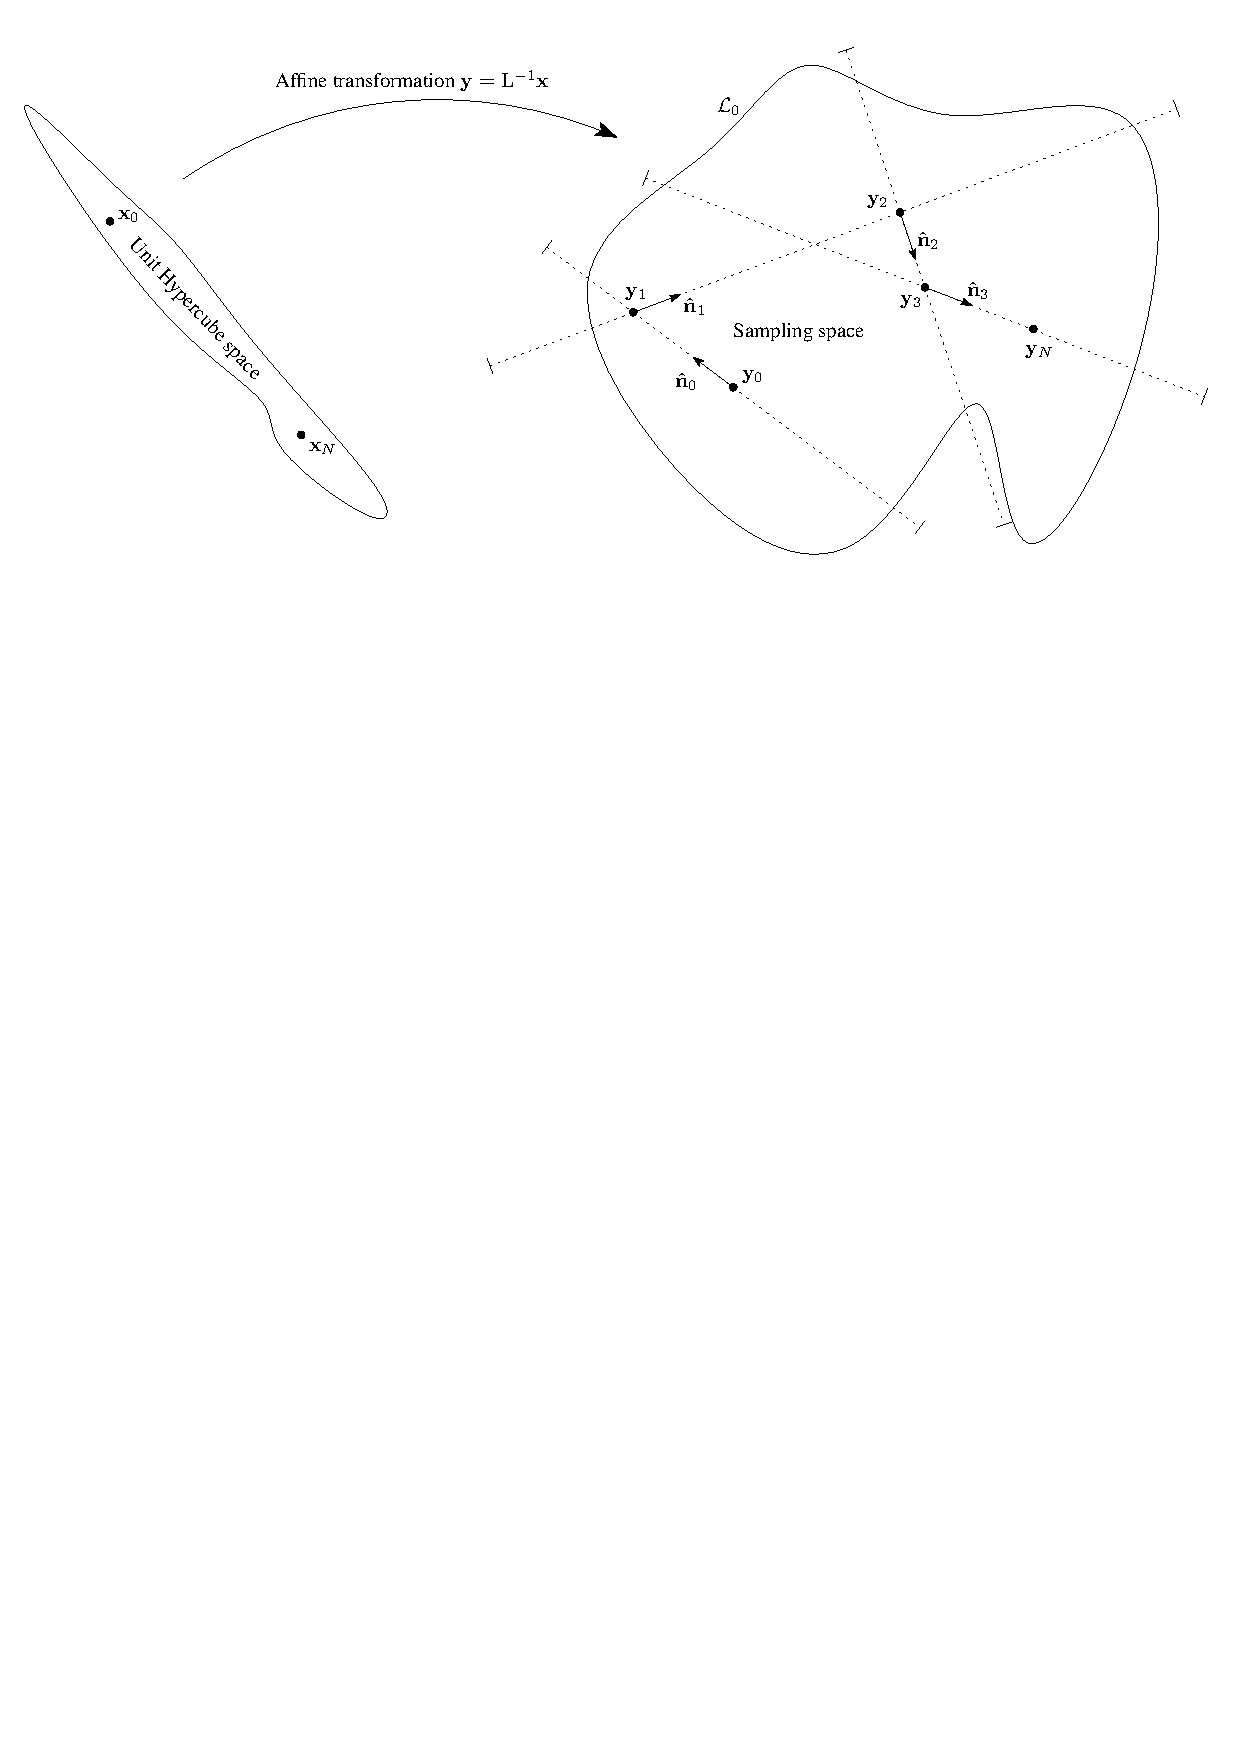
\includegraphics[width=\textwidth]{chapters/polychord/figures/contour}
}
\caption{%
  Slice sampling in \(D\) dimensions. 
  We begin by ``whitening'' the unit hypercube by making a linear transformation which turns a degenerate contour into one with dimensions \(\bigO{1}\) in all directions. 
  This is a linear skew transformation defined by the inverse of the Cholesky decomposition of the live points' covariance matrix. 
  We term this whitened space the {\em sampling space}. 
  Starting from a randomly chosen live point \(\bx{0}\), we pick a random direction and perform one-dimensional slice sampling in that direction (Appendix~\protect\ref{sec:sm:slice}), using \(w=1\) in the sampling space. 
  This generates a new point \(\bx{1}\) in \(\bigO{\text{a few}}\) likelihood evaluations. 
  This process is repeated \(\bigO{\ndims}\) times to generate a new uniformly sampled point \(\bx{N}\) which is decorrelated from \(\bx{0}\).\label{fig:pc:Nd_slice}
}
\end{figure}
%

\subsection{Multi-dimensional slice sampling}
\label{sec:pc:multi_slice}
At each iteration \(i\) of nested sampling, we generate a new randomly sampled point within the iso-likelihood contour \(\lik_i\) by our variant of \(D\)-dimensional slice sampling.
Slice sampling is performed in the unit hypercube with hypercube coordinates denoted in bold (\(\bxx\)).

At each iteration \(i\) of the nested sampling algorithm, one of the live points is chosen at random as a start point for a new chain with hypercube coordinate \(\bx{0}\). We then make a one-dimensional slice sampling step (Appendix~\protect\ref{sec:sm:slice}) with initial width \(w\) in a random direction \(\nhat{0}\) chosen from a probability distribution \(\Prob{\nhatx}\). This generates a new point \(\bx{1}\) which is uniformly sampled in the unit hypercube, but is correlated to \(\bx{0}\). This process is repeated \(\nrepeats\) times, with \(\bx{j-1}\) forming the start point for a slice along \(\nhat{j-1}\) to produce \(\bx{j}\). This procedure is illustrated in the right hand half of Figure~\ref{fig:pc:Nd_slice}.

Since the probability of drawing \(\bx{j}\) from \(\bx{j-1}\) is the same as the probability of drawing \(\bx{j-1}\) from \(\bx{j}\), this procedure satisfies detailed balance. Thus, the resulting chain will ergodically be uniformly distributed within the iso-likelihood contour. This also applies to multi-modal posteriors, with the chance of jumping out a mode being equal to the chance of jumping back in.

The length of the chain \(\nrepeats\) should be large enough so that the final point of the chain is decorrelated from the start point. 
This final point may now be considered to be a new uniformly sampled point from the prior distribution subject to the hard likelihood constraint. The intermediate points are saved and stored as phantom points. Whilst phantom points are correlated, they are useful in providing additional information and posterior points.

There are several elements of this which are left undetermined, namely the probability distribution \(\Prob{\nhatx}\), the initial width \(w\), and the chain length \(\nrepeats\). These issues are addressed in the next section.


\subsection{Contour whitening}
\label{sec:pc:cont_white}
In order to determine an optimal \(\Prob{\nhatx}\) and \(w\), an algorithm will need some knowledge of the contour in which the chain is progressing. This information can be supplied by the set of live and phantom points which are already uniformly distributed within the contour. We use the sample covariance matrix of the live and phantom points as a proxy for the size and shape of the contour.

Uniformly sampled points remain uniformly sampled under an affine transformation. The covariance matrix is used to construct an affine transformation which ``whitens'' the contour. Sampling is then performed in this whitened space, which we term the {\em sampling space}.
In the sampling space, the contour has size \(\bigO{1}\) in every direction. This means that one may choose the initial step size as \(w=1\).

To transform from \(\bxx\) in the unit hypercube to \(\byy\) in the sampling space we use the relation:
\begin{equation}
  \mathrm{L}^{-1}\bxx =  \byy,
  \label{eqn:pc:cholesky}
\end{equation}
where \(\mathrm{L}\) is the Cholesky decomposition of the covariance matrix \(\Sigma = \mathrm{L} \mathrm{L}^{T}\).
This is illustrated further in Figure~\ref{fig:pc:Nd_slice}.

Working in the sampling space our choice of \(\Prob{\nhatx}\) is inspired by the default choice of \CosmoMC{}~\citep{LewisFastSlow}. Here, a randomly oriented orthonormal basis is chosen, and these directions are chosen in a random order. Once a basis is exhausted, a new basis is chosen. This approach satisfies detailed balance, and mixes rapidly.

The choice of \(\nrepeats\) is slightly harder to justify. We find that for distributions with roughly convex contours \(\nrepeats\bigO{\ndims}\) is sufficient, with the constant of proportionality being \(2\)---\(6\). For more complicated contour shapes, one may require much larger values of \(\nrepeats\). 

This procedure has the advantage of being dynamically adaptive, and requires no tuning parameters. However, this ``whitening'' process is ineffective for pronounced curving degeneracies. This will be discussed in detail in Section~\ref{sec:pc:gaussian_shells}.


\subsection{Clustering}
\label{sec:pc:clustering}
Multi-modal posteriors are a challenging problem for any sampling algorithm. ``Perfect'' nested sampling (i.e.\ the entire prior volume enclosed by the iso-likelihood contour is sampled uniformly) in theory solves multi-modal problems as easily as uni-modal ones. In practice however, there are two issues.

First, one is limited by the resolution of the live points. If a given mode is not populated by enough live points, it runs the risk of ``dying out''. Indeed, a mode may be entirely missed if the density of live points is too low. In many cases, this problem can be alleviated by increasing the number of live points.

Second, and more importantly for \PolyChord{}, the sampling procedure may not be appropriate for multi-modal problems. We ``whiten'' the unit hypercube using the covariance matrix of live points. For far-separated modes, the covariance matrix will not approximate the dimensions of the contours, but instead falsely indicate a high degree of correlation.  It is therefore essential for our purposes to have \PolyChord{} recognise and treat modes appropriately.


This methodology splits into two distinct parts:
  (i) recognising that clusters are there, and
  (ii) evolving the clusters semi-independently.

\subsubsection{Cluster recognition}
\label{sec:pc:clustering_recognition}
Any cluster recognition algorithm can be substituted at this point.  One must take care that this is not run too often, or one runs the risk of adding a large overhead to the calculation.  In practice, checking for clustering every \(\bigO{\nlive}\) iterations is sufficient, since the prior will have only compressed by a factor \(e\).  We encourage users of \PolyChord{} to experiment with their own preferred cluster recognition, in addition to that provided and described below. 

It should be noted that the live points of nested sampling are amenable to most cluster recognition algorithms for two reasons.  First, all clusters should have the same density of live points in the unit hypercube.  Second, there is no noise (i.e.\ outside of the likelihood contour there will be no live points). Many clustering algorithms struggle when either of these two conditions is not satisfied.

We therefore choose a relatively simple variant of the \(k\)-nearest neighbours algorithm to perform cluster recognition.  If two points are within one another's \(k\)-nearest neighbours, then these two points belong to the same cluster.  We iterate \(k\) from \(2\) upwards until the clustering becomes stable (the cluster decomposition does not change from one \(k\) to the next).  If sub-clusters are identified, then this process is repeated on the new sub-clusters.

\subsubsection{Cluster evolution}
\label{sec:pc:clustering_evolution}
An important novel feature comes from what one does once clusters are identified. 

First, when spawning from an existing live point, the whitening procedure is now defined by the covariance matrix of the live points within that cluster. This solves the issue detailed above.

Second, by choosing a random initial live point as a seed, \PolyChord{} would na\"{\i}vely spawn live points into a mode with a probability proportional to the number of live points in that mode. In fact, what it should be doing is to spawn in proportion to the volume fraction of that mode. In general, these will be approximately the same, but numerical experiments show that the difference between these two ratios exhibits random-walk like behaviour, leading to biases in evidence calculations, or worse, cluster death. 

Instead, we keep track of an estimate of the volume in the same manner as equation~\eqref{eqn:pc:X_full}, and choose the mode to spawn into in proportion to that estimate. Further, one may track the errors in this estimate, which contribute to the overall evidence error. This methodology is documented fully in Section~\ref{sec:ens:evidences_clusters}.

Thus, the point to be killed off is still the global lowest-likelihood point, but we control the spawning of the new live point into clusters by using our estimates of the volumes of each cluster. We call this `semi-independent', because it retains global information, whilst still treating the clusters as separate entities. 

When spawning within a cluster, we determine the cluster assignment of the new point by which cluster it is nearest to. It does not matter if clusters are identified too soon; the evidence calculation will remain consistent.

In addition to keeping track of local volumes, we may keep track of local evidences. At the moment of splitting, the existing evidence in the initial cluster is partitioned between the new sub-clusters. Upon algorithm completion, one is left with an estimate of the proportion of the evidence contained within each cluster, and thus a measure of the importance of the various modes. By partitioning the local evidences at cluster recognition, the local evidences will sum to give the total evidences, to within the error on our inference.


\subsection{Parallelisation}
\label{sec:pc:parallelisation}
\PolyChord{} is parallelised by \openMPI{} using a master-slave structure.  One master process takes the job of organising all of the live points, whilst the remaining \({\nprocs-1}\) ``slave'' processes take the job of finding new live points. This layout is optimised for the case where the dominant cost is the generation of a new live point due to the calculation of relatively expensive likelihoods.

When a new live point is required, the master process sends a random live point and the Cholesky decomposition to a waiting slave.  The slave then, after some work, signals to the master that it is ready and returns a new live point and the intra-chain points to the master.

A point generated from an iso-likelihood contour \(\lik_i\) is usable as a new live point for an iso-likelihood contour \(\lik_j>\lik_i\), provided it is within both contours.  One may keep slaves continuously active, and discard any points returned which are not usable.  The probability of discarding a point is proportional to the volume ratio of the two contours, so if too many slaves are used, then most will be discarded.  The parallelisation goes as:
\begin{equation}
  \text{Speedup}(\nprocs) = \nlive\log\left[ 1 + \frac{\nprocs}{\nlive} \right],
  \label{eqn:pc:parallel}
\end{equation}
and is illustrated in Figure~\ref{fig:pc:parallel}. 
As a rule, \PolyChord{} parallelises well for \(\nprocs<\nlive\), but from exhibits a law of diminishing returns. In practice, \(\nprocs = \nlive/5\) yields \(\sim90\%\) parallelisation efficiency, and
since the number of live points is typically \(\sim500\), this is more than sufficient for currently available \openMPI{} architectures, and certainly superior to the parallelisation of the standard Metropolis-Hastings algorithm.
%
\begin{figure}[tp]
  \centering
  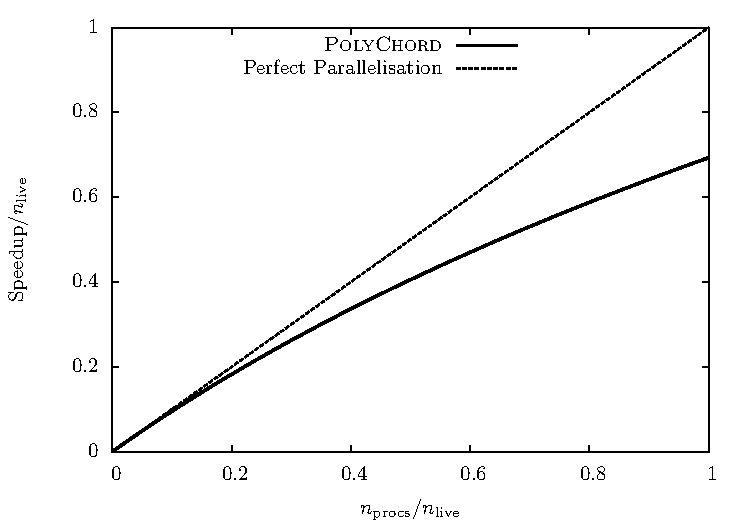
\includegraphics[width=\columnwidth]{chapters/polychord/figures/parallel}
  \caption{%
Parallelisation of \PolyChord{}. 
The algorithm parallelises nearly linearly, provided that \(\nprocs<\nlive\). For most astronomical applications this is more than sufficient.\label{fig:pc:parallel}}
\end{figure}
%
\subsection{Posterior bulking}
\label{sec:pc:posterior_bulking}
In addition to lending information on the scale and shape of a contour, phantom points can also be used as posterior samples. Correlations between samples are unimportant for the purposes of parameter estimation, provided one has enough to be well mixed. We may thus use the importance weighting detailed in~\eqref{eqn:bay:posterior_weight} with \(w_i\) being set to the volume of the live-point shell which they occupy.

For high-dimensional cosmological applications, this results in a very large number (\(\gg\)GB) of posterior samples being produced, so \PolyChord{} thins these samples. From a user's perspective, one supplies a parameter which determines the fraction of phantom points to keep.

\subsection{Fast-slow parameters and \CosmoChord}
\label{sec:pc:fast_slow}

In cosmological applications, likelihoods can exhibit a hierarchy of parameters in terms of calculation speed~\citep{LewisFastSlow}. Consequently, a likelihood may be quickly recalculated if one changes only a certain subset of the parameters. For \PolyChord{} it is very easy to exploit such a hierarchy. Our transformation to the sampling space is laid out so that if parameters are ordered from slow to fast, then this hierarchy is automatically exploited: a Cholesky decomposition, being a upper-triangular skew transformation, mixes each parameter only with faster parameters.

From a user's perspective, \PolyChord{} does this re-ordering in the hypercube automatically when provided with details of the hierarchy.

Further to this, one may use the fast directions to extend the chain length by many orders of magnitude. This helps to ensure an even mixing of live points. \PolyChord{} automatically times likelihood calculation speeds, so the user just has to provide what fraction of time \PolyChord{} should be spending on each subset of the parameters, and the algorithm will oversample accordingly.

\subsection{Tuning parameters}
\label{sec:pc:tuning_params}

From a user's perspective, the \PolyChord{} algorithm has two tuning paramaters: \(\nlive\) and \(\nrepeats\), which are detailed below.

The authors believe that these tuning parameters are fairly straightforward to set in comparison to existing algorithms. More importantly, the number of tuning parameters does not scale with the dimensionality of the problem. This is in contrast to Metropolis-Hastings and Gibbs sampling, which require a proposal matrix to be supplied\footnote{Proposal matrices may be learnt during run-time. However, this learning step can take some time and may reduce the efficacy of these approaches.}.

There are also several other options controlling run time behaviour, such as the production of equally weighted posterior samples, whether or not to perform clustering and the production and use of files allowing \PolyChord{} to resume from a previous run. These are documented in the input files supplied with the code.

\subsubsection*{Resolution \(\nlive\) }
This is a generic nested sampling parameter. \(\nlive\) indicates the number of live points maintained throughout the algorithm. Increasing \(\nlive\) causes nested sampling to contract more slowly in volume (equation~\ref{eqn:pc:X_full}), and consequently sample the space more thoroughly. Thus, it can be thought of as a resolution parameter. Run time scales \(\bigO{\nlive}\)

If set too low, posterior modes may be missed. Increasing \(\nlive\) increases the accuracy of the inference of \(\ev\), since the evidence error scales \(\bigO{\nlive^{-1/2}}\). 

\subsubsection*{Reliability \(\nrepeats\)}
This is a \PolyChord{} specific parameter. It corresponds to the length of the slice sampling chain used to generate a new live point. Increasing this parameter decreases the correlation between live points, and hence increases the reliability of the evidence inference. Posterior estimations, however, remain accurate even in the event of low \(\nrepeats\).

Setting this too low can result in correlation between live points, and unreliable evidence estimates. Typically, setting this \(\bigO{3\times\ndims}\) is sufficient, but for curving degeneracies one may need significantly longer chains. Run time scales \(\bigO{\nrepeats}\). 

The total number of live and phantom points \({\nlive\times\nrepeats}\) should be large enough that reliable covariance matrices can be calculated. Other than this, the two tuning parameters have independent effects on the algorithm. 

In general, \(\nrepeats\) should be scaled linearly with dimensionality \(D\), since one must decorrelate in \(D\) independent directions. For typical likelihoods, the logarithmic volume compression from prior to posterior will scale as \(D\). Finally, to keep evidence estimation error constant, the number of live points must be scaled with \(D\). These three effects together mean that \PolyChord{} has a theoretical run time scaling \(\bigO{D^3}\).

\section{\PolyChord{} in action}
\label{sec:pc:polychord_in_action}
We aim to showcase \PolyChord{} as both a high-dimensional evidence calculator, and multi-modal posterior sampler. We begin by comparing its dimensionality scaling with \MultiNest{}. We then demonstrate its clustering capabilities in high dimensions, and on difficult clustering problems. \PolyChord{} is shown to perform well on moderately pronounced curving degeneracies, and its implementation in \CosmoMC{} is discussed.

\subsection{High-dimensional evidences}
\label{sec:pc:hi_ev}

As an example of the strength of \PolyChord{} as a high-dimensional evidence estimator, we compare it to \MultiNest{} on a Gaussian likelihood in \(D\) dimensions.  In both cases, convergence is defined as when the posterior mass contained in the live points is \(10^{-2}\) of the total calculated evidence.  We set \(\nlive=25D\), so that the evidence error remains constant with \(D\). \MultiNest{} was run in its default mode with importance nested sampling and expansion factor \(e=0.1\).  Whilst constant efficiency mode has the potential to reduce the number of \MultiNest{} evaluations, the low efficiencies required in order to generate accurate evidences negate this effect.                                       


With these settings, \PolyChord{} produces consistent evidence and error estimates with an error \(\sim0.4\) log units (Figure~\ref{fig:pc:gaussian_evidences}). Using importance nested sampling, \MultiNest{} produces estimates that are within this accuracy.

Figure~\ref{fig:pc:gaussian} shows the number of likelihood evaluations \(\nlike\) required to achieve convergence as a function of dimensionality \(D\). 
Even on a simple likelihood such as this, \PolyChord{} shows a significant improvement over \MultiNest{} in scaling with dimensionality.  \PolyChord{} at worst scales as \({\nlike\bigO{D^3}}\), whereas \MultiNest{} has an exponential scaling which emerges in higher dimensions.
However, we must point out that a good rejection algorithm like \MultiNest{} will always win in low dimensions. We therefore recommend using \MultiNest{} for low dimensional problems, although it should be noted that \MultiNest{}'s clustering is ineffective in modest dimensionalities.

\begin{figure}[tp]
  \centering
  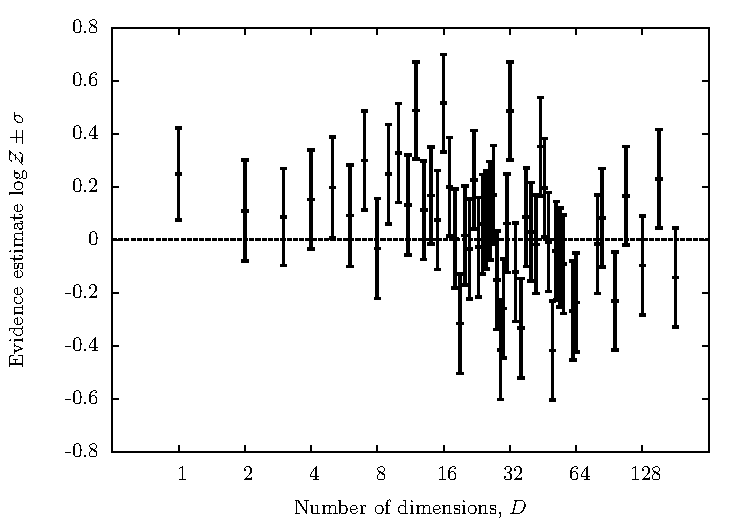
\includegraphics[width=\columnwidth]{chapters/polychord/figures/gaussian_evidences}
  \caption{%
    Evidence estimates and errors produced by \PolyChord{} for a Gaussian likelihood as a function of dimensionality. The dashed line indicates the correct analytic evidence value.\label{fig:pc:gaussian_evidences}
}
\end{figure}

\begin{figure}[tp]
  \centering
  \includegraphics[width=\columnwidth]{chapters/polychord/figures/gaussian}
  \caption{Comparing \PolyChord{} with \MultiNest{} using a Gaussian likelihood for different dimensionalities. \PolyChord{} has at worst \(\nlike\bigO{D^3}\), whereas \MultiNest{} has an exponential scaling that emerges at high dimensions.}\label{fig:pc:gaussian}
\end{figure}

\subsection{Clustering and local evidences}
\label{sec:pc:loc_ev}
To demonstrate \PolyChord{}'s clustering capability we report its performance on a ``Twin Peaks'' and Rastrigin likelihood.

\subsubsection{Twin peaks}
\label{sec:pc:twin_peaks}
\PolyChord{} is capable of clustering posteriors in very high dimensions. We define a twin peaks likelihood as an equal mixture of two spherical Gaussians, separated by a distance of 10\(\sigma\).

\PolyChord{} correctly identifies these clusters in arbitrary dimensions (tested up to \(D=100\)), provided that \(\nlive\) and \(\nrepeats\) are scaled in proportion to \(D\). It calculates a global evidence that agrees with the analytic results. In addition, the local evidences correctly divide the peaks in proportion to their evidence contribution.

The results for a twin peaks likelihood are of an identical character to Figures~\ref{fig:pc:gaussian_evidences}~\&~\ref{fig:pc:gaussian}, and hence not included.

\subsubsection{Rastrigin function}
\label{sec:pc:rastrigin}

\begin{figure}[tp]
  \centering
  \includegraphics[width=\columnwidth]{chapters/polychord/figures/rastrigin}
  \caption{The two-dimensional Rastrigin \(\log\)-likelihood in the range \({[-1.5,1.5]}^2\). Within this region there are \(8\) local maxima, and one global maximum at \((0,0)\). The clustered samples produced by \PolyChord{} are plotted on the \(\log\)-likelihood surface, with colours that indicating the separate clusters identified.}\label{fig:pc:rastrigin}
\end{figure}

\begin{figure}[tp]
  \centering
  \includegraphics[width=\columnwidth]{chapters/polychord/figures/rastrigin_data}
  \caption{\PolyChord{} cluster identification for the Rastrigin function. \PolyChord{} identifies posterior modes and computes their local evidences, expressed here as a logarithmic fraction of  the total evidence in the mode. Dashed lines indicate the analytic results computed by a saddle point approximation at each of the peaks. As can be seen, \PolyChord{} reliably identifies the inner \(21\) modes with increasing accuracy.}\label{fig:pc:rastrigin_data}
\end{figure}

\PolyChord{}'s clustering capacity is very effective on complicated clustering problems as well. The \(n\)-dimensional Rastrigin test function is defined by:
\begin{align}
  f(\theta) &= A n + \sum\limits_{i=1}^n \left[\theta_i^2 - A\cos(2 \pi \theta_i) \right],
  \label{eqn:pc:rastrigin_function}
  \\
  A&=10, \qquad \theta_i \in [-5.12,5.12]. \nonumber
\end{align}
This is the industry standard ``bunch of grapes'', the two-dimensional version of which is illustrated in Figure~\ref{fig:pc:rastrigin}.
For our purposes, we will treat~\eqref{eqn:pc:rastrigin_function} as the negative log-likelihood so that \(\lik(\theta) \propto \exp[-f(\theta)]\).
This is a stereotypically hard problem to solve, as many algorithms get stuck in local maxima.



We ran \PolyChord{} on a two-dimensional Rastrigin log-likelihood  with \(\nlive=1000\) and \(\nrepeats=6\). With these settings, \PolyChord{} calculates accurate evidence and posterior samples (Figure~\ref{fig:pc:rastrigin}), and in addition correctly isolates and computes local evidences for the inner \(21\) modes. Additional outer modes are also found, but these are combinations of lower modes due to their very low posterior fraction. Increasing the resolution parameter \(\nlive\) further increases the number of modes identified.  Examples of clustered posterior samples are indicated in Figure~\ref{fig:pc:rastrigin_data}, coloured using \citepos{cubehelix} `cubehelix'.


\subsection{Rosenbrock function}
\label{sec:pc:rosenbrock}

\begin{figure}[tp]
  \centering
  \includegraphics[width=\columnwidth]{chapters/polychord/figures/rosenbrock_analytic}
  \caption{Density plot of the two-dimensional Rosenbrock function. The function exhibits a long, thin curving degeneracy, with a global maximum at \((1,1)\).}\label{fig:pc:rosenbrock_2d}
\end{figure}

\begin{figure}[tp]
  \centering
  \includegraphics[width=\columnwidth]{chapters/polychord/figures/rosenbrock}
  \caption{The four-dimensional Rosenbrock posterior, with \(x_3\) and \(x_4\) marginalised out. \PolyChord{} correctly identifies both the local (red) and global (blue) maxima.}\label{fig:pc:rosenbrock}
\end{figure}

\PolyChord{} is also capable of navigating moderate curving degeneracies. 

The \(n\)-dimensional Rosenbrock function is defined by:
\begin{align}
  f(x) &= \sum\limits_{i=1}^{n-1}   {(a-x_i)}^2+ b {(x_{i+1} -x_i^2 )}^2,
    \label{eqn:pc:rosenbrock}
    \\
    a&=1,\quad b=100,\quad x_i\in[-5,5],
\end{align}
the two-dimensional version of which is plotted in Figure~\ref{fig:pc:rosenbrock_2d}. This is the industry standard ``banana'', as it exhibits an extremely long and flat curving degeneracy. We consider \({n=4}\), in which there is a global maximum at \((1,1,1,1)\) and a local maximum at \((-1,1,1,1)\). The true evidence value is \(-15.1091\), and with \(\nlive=1000,\nrepeats=12\), \PolyChord{} reliably finds both peaks (Figure~\ref{fig:pc:rosenbrock}) and produces a correct evidence estimation.

In higher dimensions, \PolyChord{} reliably finds the local and global maxima. The lack of an analytic evidence value for the Rosenbrock function prevents a verification of the evidence calculation.

\subsection{Gaussian shells}
\label{sec:pc:gaussian_shells}

A ``Gaussian shell'' with mean \(\bmew\), radius \(r\) and width \(w\) is defined as:
\begin{equation}
  \log\lik_\sshell(\bxx|\bmew,r,w) = A - \frac{{\left(\left|\bxx - \bmew\right|- r\right)}^2}{2w^2},
  \label{eqn:pc:gaussian_shell}
\end{equation}
where \(A\) is a normalisation constant that may be calculated using a saddle point approximation.
This likelihood is centered on some mean vector \(\bmew\), and has a radial Gaussian profile with width \(w\) at distance \(r\) from this centre. This radial profile is then revolved around \(\bmew\) to create a spherical shell-like likelihood. A two-dimensional version of this likelihood is indicated in Figure~\ref{fig:pc:gaussian_shell}.

This distribution may be representative of likelihoods that one may encounter in beyond-the-Standard-Model paradigms in particle physics. In such models, the majority of the posterior mass lies in thin sheets or hypersurfaces through the parameter space.

Running \PolyChord{} on a \(100\)-dimensional Gaussian shell with \(\nlive=1000\), \(\nrepeats=200\) yields consistent evidences and posteriors, shown in Figure~\ref{fig:pc:gaussian_shell_posterior}. 
                                                                  
Given that this problem is quoted as being ``optimally difficult'' \citep{MultiNest2}, the ease with which \PolyChord{} tackles this problem in high dimensions is worth explanation. In the two-dimensional case, it is clear that the posterior mass is concentrated in a very thin, curving region of the parameter space. However, as the dimensionality is increased, more and more of the \(n\)-sphere's volume is concentrated at the edge, and the thin characteristic of the degeneracy is lost. 

This may mean that the Gaussian shell is not a good proxy for a high-dimensional curving degeneracy. However, it could equally suggest that curving degeneracies become easier to navigate in higher dimensions. We can certainly conclude that a particle physics model with a proliferation of phases would be easier to navigate than one with a smaller number of phases.


\begin{figure}[tp]
  \centering
  \includegraphics[width=\columnwidth]{chapters/polychord/figures/gaussian_shell}
  \caption{The two-dimensional Gaussian shell likelihood.}\label{fig:pc:gaussian_shell}
\end{figure}

\begin{figure}[tp]
  \centering
  \includegraphics[width=\columnwidth]{chapters/polychord/figures/gaussian_shell_posterior}
  \caption{Posteriors produced by \PolyChord{} for a \(n=100\)-dimensional Gaussian shell, with width \(w=0.1\), radius \(r=2\), and center \(\bmew=\bzero\).  Plotting the marginalised posteriors for the Cartesian sampling parameters \({\{x_1,\ldots,x_n\}}\) yields Gaussian distributions centered on the origin. To see the effectiveness of the sampler it is better to plot the sampling parameters in terms of \(n\)-dimensional spherical polar coordinates \({\{r,\phi_1,\ldots,\phi_{n-1}\}}\). Note that the polar coordinates are {\em derived parameters}, and that the sampling space still has the strong Gaussian shell degeneracy.  In this case we can see that the radial coordinate has a Gaussian profile centered on \(r_0 = r\times\frac{1}{2} {\left(1 + \sqrt{1 +  4 (n-1) {\left({w}/{r}\right)}^2}\right) }\) with width \(w_0 = w{(1+(n-1){(w/r_0)}^2)}^{-1/2}\).  The azimuthal coordinate \(\phi_{n-1}\) has a uniform posterior, and the other angular coordinates \(\{\phi_i\}\) have posteriors defined by \(\Prob{\phi_i } \propto {{\left(\sin\phi_i\right)}^{n-i-1}}\).}\label{fig:pc:gaussian_shell_posterior} 
\end{figure}


\subsubsection{Twin Gaussian shells}
We finish our toy problems by combining the difficulties of multimodality (Section~\ref{sec:pc:loc_ev}) and degeneracy, by mixing two twin Gaussian shells together:
\begin{equation}
  \lik(\bxx) \propto \lik_\sshell(\bxx|\bmew_1,r,w) + \lik_\sshell(\bxx|\bmew_2,r,w).
  \label{eqn:pc:gaussian_shells}
\end{equation}
We choose \(r=2\), \(w=0.1\), and \(\mu_1\) and \(\mu_2\) are separated by \(7\) units. With \(\nlive=10\ndims\) and \(\nrepeats=2\ndims\), \PolyChord{} successfully computes the local and global posteriors and evidences up to \(D=100\), and reliably identifies the two modes. The comparison of run times with \MultiNest{} recovers a similar pattern to Figure~\ref{fig:pc:gaussian}, although in our experience, the \MultiNest{} parameters require some tuning to ensure that evidences are calculated correctly when \(\ndims>30\).


\subsection{\CosmoChord}
\label{sec:pc:cosmochord}

\begin{figure}[tp]
  \centering
  \includegraphics[width=\textwidth]{chapters/polychord/figures/cosmochord}
  \caption{\CosmoChord{} (red) vs.\ \CosmoMC{} (black). We use the 2013 {\texttt CAMSPEC}+{\texttt commander} likelihoods with a standard six-parameter \(\Lambda\)CDM cosmology, varying all 14 nuisance parameters.  We compare the \(1\) and \(2\)-dimensional marginalised posteriors of the \(6\) \(\Lambda\)CDM parameters. \CosmoChord{} is in close agreement with the posteriors produced by \CosmoMC{}, recovering the correct mean values of and degeneracies between the parameters. The slight deviations between the red and black curves are sampling noise.}\label{fig:pc:cosmochord}
\end{figure}

An additional strength of \PolyChord{} lies in its ability to exploit a fast-slow hierarchy common in many cosmological applications. 

As an example, we consider the likelihoods provided by \CAMB{}~\citep{CAMB} and \CosmoMC{}~\citep{cosmomc}. In Boltzmann codes such as \CAMB{}, parameters controlling the primordial power spectrum (such as \(n_s\) and \(A_s\)) do not require recalculation of transfer functions. These parameters are termed ``semi-slow''. In addition, modern Planck likelihoods~\citep{Planck2013Like} have nuisance parameters associated with the foregrounds. These may be varied without recalculation of the cosmological background. These parameters are hence termed ``fast''. \CosmoMC{}~\citep{cosmomc} implements this hierarchy of speeds in its likelihood calculation.

We have successfully implemented \PolyChord{} within \CosmoMC{}, and term the result \CosmoChord{}.  The traditional Metropolis-Hastings algorithm is replaced with nested sampling. This implementation is available to download from the link at the end of the chapter.

The exploitation of fast-slow parameters means that \CosmoChord{} vastly outperforms \MultiNest{} when running with modern Planck likelihoods. 

\CosmoMC{} by default uses a Metropolis-Hastings sampler. If this has a well-tuned proposal distribution (e.g.\ if one is performing importance sampling from an already well-characterised likelihood), then \PolyChord{} is \(2\)--\(4\) times slower than the traditional \CosmoMC{}. If proposal matrices are unavailable (e.g.\ in the case that one is examining an entirely new model) then \CosmoChord{}'s run time is competitive with the native \CosmoMC{} sampler. This is a good example of the self-tuning capacity of \PolyChord{}, since it only requires two tuning parameters, as opposed to \(\bigO{D^2}\).

\CosmoChord{} produces parameter estimations consistent with \CosmoMC{} (Figure~\ref{fig:pc:cosmochord}).
It has been implemented effectively in multiple cosmological applications in the latest Planck paper describing constraints on inflation~\citep{planck2015-a24}, including application to a \(37\)-parameter reconstruction problem (\(4\) slow, \(19\) semi-slow, \(14\) fast). 
In addition, \PolyChord{} is an integral component of the \ModeChord{} code, a combination of \CosmoChord{} and \ModeCode{} \citep{ModeChord1,ModeChord2,ModeChord3}, which is available at \url{http://modecode.org/}.

\section{Conclusions}
\label{sec:pc:conclusions}
We have introduced \PolyChord{}, a novel nested sampling algorithm tailored for high-dimensional parameter spaces. It is able to fully exploit a hierarchy of parameter speeds such as is found in \CosmoMC{} and \CAMB{}. It utilises slice sampling at each iteration to sample within the hard likelihood constraint of nested sampling. It can identify and evolve separate modes of a posterior semi-independently and is parallelised using \openMPI{}.












\section*{Download Link}
PolyChord is available for download from:\\ \url{http://ccpforge.cse.rl.ac.uk/gf/project/polychord/}



%
% RKWKB
% -----
%
\chapter[The RKWKB method]{The Runge-Kutta-Wentzel-Kramers-Brillouin~method}
\label{chp:RK}

\section{Introduction}
\label{sec:introduction}
The numerical solution of linear, ordinary differential equations is of critical importance throughout science and mathematics. In this chapter we suggest an efficient approach for navigating highly oscillatory numerical solutions.

Most traditional numerical solvers of differential equations use a generalisation of Runge-Kutta (RK) techniques \citep{Press+2007}. These apply Taylor's theorem to create a stepping scheme whereby the value of the solution is updated using derivative information. Good solvers will also incorporate adaptive step-size control.
Whilst RK techniques are an excellent workhorse for solving a wide variety of problems, they are known to struggle to solve equations with highly oscillatory solutions.

On the other hand, the Wentzel-Kramers-Brillouin (WKB) method is a well established analytical approach for approximately describing oscillatory solutions \citep{RHB,Bender+2010}. Historically this has been used to approximate the global shape and characteristics of an oscillating solution with a ``slowly changing'' frequency.

We propose that one may combine the two approaches to create a reliable general tool for the numerical solution of oscillatory differential equations, and term the result RKWKB\footnote{Readers with experience in the field will note that, as Cambridge authors, we should be insisting on an additional `J' in WKB (for Jeffreys). Given the length of our proposed acronym, we have opted to use the more efficient nomenclature.}.

We note that this approach is similar to the work of~\cite{Iserles02globalerror,Iserles01thinkglobally}, and explore the similarities and differences in Section~\ref{sec:iserles_comparison}.


\section{Background}
\subsection{Oscillating solutions}
We seek to create a numerical method which efficiently solves linear differential equations such as:
\begin{equation}
  \ddot{x}(t) + {\omega(t)}^2x(t) = 0,\qquad \omega(t)\in\mathbb{R}.
  \label{eqn:lode}
\end{equation}
If \(\omega(t)=\omega = \mathrm{constant}\), then the solutions are sinusoidal: \(x\propto \exp{(\pm i \omega t)}\). If \(\omega(t)\) changes slowly with \(t\), then the solutions are approximately sinusoidal with a slowly varying frequency and amplitude (these ideas will be made more concrete in Section~\ref{sec:wkb}). An example of such a solution can be seen in Figure~\ref{fig:airy}.

In general, any second order linear differential equation may be transformed into the form of~\eqref{eqn:lode} by either changing the independent variable \(t\) or dependent variable \(x\). The method we shall describe can easily be adapted to other linear differential equations, but we shall work with~\eqref{eqn:lode} for its simplicity of exposition.

Equation~\eqref{eqn:lode} is ubiquitous in physics, particularly in quantum mechanics. The authors' particular interest in its efficient solution comes from work in quantum fields in curved spacetime.



Over the next two subsections we will review the traditional techniques available for solving equations such as~\eqref{eqn:lode}.

\begin{figure}[tp]
  \centering
  \includegraphics[width=\textwidth]{chapters/RKWKB/figures/airy}
  \caption{The real and imaginary parts of the function \(\mathrm{Ai}(-t) + \mathrm{Bi(-t)} i\), where \(\mathrm{Ai}\) and \(\mathrm{Bi}\) are the Airy functions of the first and second kind. This is a solution to the equation \({\ddot{x}(t) + t x(t) = 0}\) (equation~\ref{eqn:airy_equation}).}\label{fig:airy}
\end{figure}


\subsection{Runge-Kutta theory}
\label{sec:rk}
We briefly review the theory of numerically solving ordinary differential equations, before discussing why Runge Kutta techniques are an inefficient tool for solving equations such as~\eqref{eqn:lode}.
For a more detailed introduction to the numerical solution of ordinary differential equations we recommend~\cite{Press+2007}.

A general non-linear differential equation in \(n\) variables can be written in terms of vectors as:
\begin{equation}
  \dot{\mathbf{y}}(t) = \mathbf{f}(\mathbf{y}(t),t).
  \label{eqn:ode}
\end{equation}
Note that any higher order differential equation can be re-written in this form by introducing new variables for each of the higher derivative terms.

Runge-Kutta methods work effectively by generalising the Taylor expansion:
\begin{equation}
  \mathbf{y}(t+h)  = \mathbf{y}(t) + h\:\mathbf{f}(\mathbf{y}(t),t) + \mathcal{O}(h^2).
  \label{eqn:euler}
\end{equation}
Given the value of a solution \(\mathbf{y}_j\) at some time \(t_j\), one may advance to the value of the solution \(\mathbf{y}_{j+1}\) at some finite time later \(t_{j+1} = t_j + h\) by using the recursion relation:
\begin{align}
  \mathbf{y}_{j+1} &=  \mathbf{y}_{j} + h\:\mathbf{f}(\mathbf{y}_j,t_j),
  \label{eqn:y_step}\\
  t_{j+1} &=  t_{j} + h.
  \label{eqn:t_step}
\end{align}
This is termed {\em Euler's method}, and for arbitrarily small \(h\) will recover the solution to any desired accuracy. It is termed {\em first order\/} since each step is accurate to \(\bigO{h}\).

Euler's method is normally impractical for real numerical work. Runge-Kutta schemes work by generalising~\eqref{eqn:euler}~\&~\eqref{eqn:y_step} by including additional intermediate function evaluations that integrate~\eqref{eqn:ode} with greater accuracy.

A possibly more important adjustment is to equip the algorithm with the ability to choose the step size \(h\) according to the accuracy required. A popular stratagem is to run two steps, one of order \(p\), and another of order \(p-1\), and use the difference between the two as an estimate of the error. Particularly smart algorithms use the same function evaluations for both orders. An example of this is the Runge-Kutta-Fehlberg \(4(5)\) method detailed in Section~\ref{sec:rkf}.

All methods based on this principle struggle to solve equations such as~\eqref{eqn:lode} when the algorithm must scale a very large number of peaks and troughs. Errors accumulate rapidly in these approaches, even if the variation of \(\omega(t)\) in \(t\) is very simple. Given the regularity of the solution from Figure~\ref{fig:airy}, one would imagine that there should be a more efficient method.


\subsection{WKB theory}
\label{sec:wkb}
WKB approaches are designed to solve linear ordinary differential equations like~\eqref{eqn:lode} in the limit of a ``slowly varying'' \(\omega(t)\): i.e.\ the fractional change in frequency \(\frac{\Delta\omega}{\omega}\) over several time periods \(\Delta t \sim \frac{2\pi}{\omega}\) is relatively small.
A systematic way of phrasing this is to rescale the independent variable of~\eqref{eqn:lode} so \(t\rightarrow T t\):
\begin{equation}
  \ddot{x}(t) + T^2{\omega(t)}^2x(t) = 0,\qquad \omega(t)\in\mathbb{R}.
  \label{eqn:lode_T}
\end{equation}
If \(T\gg1\) then \(\omega\) is slowly varying, or equivalently the solutions have very rapid oscillations (large \(\omega\)). Given this, one can expand the solutions in terms of complex exponential functions:
\begin{equation}
  x(t)\sim \exp\left( \frac{1}{T}\sum\limits_{n=0}^{\infty} S_n(t)\: T^n \right).
  \label{eqn:asymp}
\end{equation}
Substituting this into~\eqref{eqn:lode_T} and setting each coefficient of \(T\) equal to zero yields a sequence of solvable equations. One finds the first four solutions are:
\begin{align}
  S_0(t) &= \pm i \int^t \omega(\tau)\: \d{\tau},
  \label{eqn:S0}\\
  S_1(t) &= -\frac{1}{2}\log \omega(t),\\
  S_2(t) &=  i \int^t \frac{1}{4}\frac{\ddot{\omega}(\tau)}{\omega^{2}(\tau)} - \frac{3}{8}\frac{\dot{\omega}^2(\tau)}{\omega^{3}(\tau)}\: \d{\tau}, \\
  S_3(t) &=  \frac{1}{8}\frac{\ddot{\omega}(t)}{\omega^{3}(t)} - \frac{3}{16} \frac{\dot{\omega}^{2}(t)}{\omega^{4}(t)}.
\end{align}
Note that at \(0\)\textsuperscript{th} order, the solution is \(x\propto\exp\left( \int \omega \d{t} \right)\), which should be compared with the traditional sinusoidal solution.
Typically \(T\) is considered a power counting parameter, and set equal to \(1\) at the end of the analysis.

There are two integration constants associated with the either sign of equation~\eqref{eqn:S0}. The other integration constants from the remaining equations may be absorbed into the first two. The \(n\)\textsuperscript{th} order solution thus takes the form:
\begin{align}       
  x_\mathrm{WKB}^{(n)}[A_{\pm}](t) &=
  A_{+} e^{\phi_+(t)} + A_{-} e^{\phi_-(t)},
  \label{eqn:solution} \\
  \phi_\pm(t) &= \pm S_0(t) + S_i(t).
  \label{eqn:phidef} 
\end{align}
If one has initial conditions at time \(t_0\):
\begin{equation}
  x(t_0) = x_0, \qquad \dot{x}(t_0)=\dot{x}_0,
  \label{eqn:i_c}
\end{equation}
then the coefficients \(A_\pm\) may be determined by:
\begin{equation}
  A_\pm^{(n)}(x_0,\dot{x}_0,t_0) = \pm\frac{\dot{x}_0 - x_0 \phi_\mp(t_0)}{2\dot{S}_0(t_0)} e^{-\phi_\pm(t_0)}.
  \label{eqn:i_c_Apm}
\end{equation}
We can perform the same analysis with the derivative of~\eqref{eqn:asymp}:
\begin{equation}       
  \dot{x}_\mathrm{WKB}^{(n)}[B_{\pm}](t) =
  B_{+} \dot{\phi}_+(t)e^{\phi_+(t)} + B_{-} \dot{\phi}_-(t)e^{\phi_-(t)}.
  \label{eqn:solution_xdot}
\end{equation}
If one has initial conditions at time \(t_0\):
\begin{equation}
  \dot{x}(t_0) = \dot{x}_0, \qquad \ddot{x}(t_0)=\ddot{x}_0,
  \label{eqn:i_c_xdot}
\end{equation}
then the coefficients \(B_\pm\) may be determined by:
\begin{equation}
  B_\pm^{(n)}(\dot{x}_0,\ddot{x}_0,t_0) = 
  \pm\frac{%
    \dot{x}_0(\ddot{\phi}_\mp- \dot{\phi}_\mp^2)-\ddot{x}_0 \dot{\phi}_\mp
  }{%
    \dot{\phi}_+ \ddot{\phi}_- -\ddot{\phi}_+ \dot{\phi}_- +\dot{\phi}_+ \dot{\phi}_-^2-\dot{\phi}_+^2 \dot{\phi}_-} e^{-\dot{\phi}_\pm},
  \label{eqn:i_c_Bpm}
\end{equation}
where all \(\phi\) variables are evaluated at \(t_0\).


For further detail on the intricacies of WKB approaches, the reader should consult~\cite{RHB,Bender+2010}.

\section{The RKWKB method}
Our strategy is to combine the versatility of RK methods with the power of WKB in dealing with oscillating solutions. We term the combination RKWKB\@.

Given a function \(\omega(t)\), one proposes a step in time of \(h\) to be accompanied by an updating of the solution \(x_j\) via:
\begin{align}
  x_{j+1} &= x_\mathrm{WKB}^{(n)}[A_\pm(x_j,\dot{x}_j,t_j)](t_j+h),
  \label{eqn:WKB_x_step} \\
  \dot{x}_{j+1} &= \dot{x}_\mathrm{WKB}^{(n)}[B_\pm(\dot{x}_j,\ddot{x}_j,t_j)](t_j+h),
  \label{eqn:WKB_xdot_step} \\
  t_j &= t_j+h,
  \label{eqn:WKB_t_step} \\
  \ddot{x}_{j+1} &= -\omega^2(t_{j+1})x_{j+1}
  \label{eqn:WKB_xddot} 
\end{align}
where \(x_\mathrm{WKB}^{(n)}[A_{\pm}]\) and \(\dot{x}_\mathrm{WKB}^{(n)}[B_{\pm}]\) are given by~\eqref{eqn:solution} and~\eqref{eqn:solution_xdot},  and \(A_{\pm}\) and \(B_{\pm}\)  are given by~\eqref{eqn:i_c_Apm} and~\eqref{eqn:i_c_Bpm}.

To paraphrase the above; one matches the \(n\)\textsuperscript{th} order WKB solution onto the current values of \(x_j\) and \(\dot{x}_j\), and uses this to extrapolate the solution by a time step of \(h\). We repeat the same process for the derivative \(\dot{x}_j\), using its own WKB expansion. Finally, we self-consistently fix \(\ddot{x}_j\) so that it satisfies equation~\eqref{eqn:lode}. Since WKB naturally encodes the oscillatory nature of the solution, this will allow step sizes \(h\) to be far larger than a single period of oscillation. 

Note the importance of using two WKB expansions with coefficients \(A_\pm\) and \(B_\pm\) to step \(x_j\) and \(\dot{x}_j\) separately. If we used the same coefficients to step both, then one would simply be following the same WKB solution.

\subsection{Step size adjustment}
To tune the step size \(h\), we use the same strategy as adaptive Runge-Kutta schemes. We compute both the order \(n\) and order \(n-1\) WKB solutions, and use the fractional difference between the two:
\begin{equation}
  \varepsilon = \left|\frac{x^{(n)}-x^{(n-1)}}{x^{(n)}}\right|,
  \nonumber
\end{equation}
as an estimate of the truncation error. 

We now assume that the desired accuracy is \(\alpha\). If \(\varepsilon<\alpha\) then the solution is within the desired tolerance, and the algorithm makes a step of size \(h\). \(h\) is then increased for the next iteration. If \(\varepsilon>\alpha\) then the step is unsuccessful, and the step size is reduced. \(h\) may therefore be efficiently updated between attempts via:
\begin{equation}
  h \to h\times\left\{
  \begin{array}{lr}
    {(\alpha/\varepsilon)}^{1/n} &: \varepsilon<\alpha \\
    {(\alpha/\varepsilon)}^{1/(n-1)} &: \varepsilon>\alpha. \\
  \end{array}
  \right.\label{eqn:h_update}
\end{equation}
This allows the step size to increase in the regions where the initial step size is unnecessarily small, whilst ensuring that the step size is always small enough to keep forecasts within a given error margin.

\subsection{Dynamic switching}
In general, one cannot expect the WKB expansion to be efficient throughout the solution region. If \(\omega\) is too small, or too quickly varying, then the step size \(h\) will decrease to an inefficiently small size. This problem can be countered by simultaneously attempting a step using a standard adaptive RK method. One chooses between RK and WKB by selecting the method with the smallest error. This provides a natural switching mechanism, without having to delve into the details of whether WKB is valid or not.

We choose the Runge-Kutta-Fehlberg \(4(5)\) method for our alternative solver, which is detailed in Section~\ref{sec:rkf}. However, this may be substituted with any ODE solver according to the users preference.

\section{Example: The Airy equation}


As an example of the RKWKB approach, we apply it to the Airy equation:
\begin{align}
  0=\ddot{x}(t) &+ t\: x(t) ,
  \label{eqn:airy_equation}\\
  x(0)=\frac{3^{-2/3}+3^{-1/6}i}{\Gamma(2/3)},
  &\qquad
  \dot{x}(0) = \frac{3^{-1/3}-3^{1/6}i}{\Gamma(1/3)},
  \nonumber\\
  \Rightarrow x(t) = \mathrm{Ai}(-t) &+ \mathrm{Bi}(-t)\:i,
  \label{eqn:airy_solution}
\end{align}
whose solution is depicted in Figure~\ref{fig:airy}. This is often quoted as being a ``maximally hard'' problem for RK machinery to solve, since the frequency steadily increases, causing the step size to get smaller as the algorithm goes deeper into the solution.

We set the desired relative error to be \(10^{-4}\). The algorithm remains in the RK regime until \(t\sim5\). When the WKB solver is activated, instead of following every oscillation of the solution, it rapidly speeds up, skipping many oscillations. This is detailed in Figure~\ref{fig:data}.

The error compared to the true solution is detailed in Figure~\ref{fig:error}. Here we find that initially the error is small, but grows\(\bigO{h^{2s} t^{s+5/4}}\) where \(s=4\) is the order of the RK method \citep{Iserles02globalerror}. After the WKB regime is entered, it begins to make huge strides, and the error levels off.

In contrast to a ``pure'' RK method, the RKWKB method finds the Airy equation maximally {\em easy}.



\begin{figure}[tp]
  \centering
  \includegraphics[width=\textwidth]{chapters/RKWKB/figures/data}
  \caption{The RKWKB method compared with the analytical solution. The algorithm starts at \(t=0\) in the RK regime, since \(\omega\) is varying quickly relative to the oscillation period. At \(t=5\) it becomes more efficient to use the WKB regime, and the points start to increase in separation. By \(t=15\) the algorithm is skipping multiple periods, and the step size \(h\) increases exponentially.}\label{fig:data}
\end{figure}

\begin{figure}[tp]
  \centering
  \includegraphics[width=\textwidth]{chapters/RKWKB/figures/error}
  \caption{Fractional difference between the analytical solution and RKWKB solution from Figure~\protect\ref{fig:data}. The algorithm's fractional error begins at \(t=0\) with an error of \(\sim10^{-4}\), but rises in the RK phase. This is to be expected as RK methods accumulate errors (particularly for oscillatory solutions). Upon entering the WKB region, the fractional error levels off. Note the rapidly increasing step size, and accuracy at extremely late times \(t\). To the authors' knowledge, no numerical scheme to date has demonstrated the ability to solve the Airy equation~\protect\eqref{eqn:airy_equation} to times as late as this.}\label{fig:error}
\end{figure}




\section{Comparison with the Iserles approach}
\label{sec:iserles_comparison}
Iserles has written extensively on the difficulty of solving problems of the form~\eqref{eqn:lode}. His approach is to turn~\eqref{eqn:lode} into a Lie-group differential equation \citep{Iserles00lie-groupmethods} by writing:
\begin{align}
  \mathbf{y} &= {(x,\dot{x})}^\top, 
  \mathrm{A}(t) = 
  \left(
  \begin{array}{cc}
    0 & 1 \\
    -\omega^2(t) & 0
  \end{array}
  \right),
  \nonumber\\
  \Rightarrow\quad 
  \dot{\mathbf{y}} &= \mathrm{A} (t) \: \mathbf{y}.\label{eqn:lie_eqn}
\end{align}
This may then be attacked with a variety of Lie group methods. For example, one may write the full solution as a Magnus expansion:
\begin{align}
  \mathbf{x}(t) &= e^{\Omega(t,t_0)} \mathbf{x}_0,
  \label{eqn:magnus}\\
  \Omega(t,t_0) &= \int_{t_0}^t \mathrm{A}(x) \d{x} \nonumber \\
  &- \frac{1}{2}\int_{t_0}^t\int_{t_0}^{x_1} \left[\mathrm{A}(x_2),\mathrm{A}(x_1)\right] \d{x_2} \d{x_1} + \ldots
  \nonumber
\end{align}
and then use a truncated series to create a stepping algorithm.
This approach is much improved by transferring to a fast rotating frame:
\begin{equation}
  \mathbf{y}(t_n+\tau) = e^{\tau \mathrm{A}(t_n+h/2)} \mathbf{x},
  \label{eqn:rotating_frame}
\end{equation}
the end product is then termed the {\em modified Magnus method\/} \citep{Iserles01thinkglobally}.

The RKWKB method and the modified Magnus method share some key features. Indeed, the lowest order modified Magnus method is equivalent to a \(1\)\textsuperscript{st} order WKB approach \citep{Iserles02globalerror}. However, our approach is distinguished in several ways. 

First, the Magnus expansion~\eqref{eqn:magnus} requires multiple integrals for higher order terms. These integrals are tricky to implement, and can introduce considerable computational overhead. The WKB expansion~\eqref{eqn:WKB_x_step} on the other hand requires at most single integrals, replacing the double integrals with additional derivative terms of \(\omega\), which are typically easier to compute.

Second, our approach uses adaptive step-size control, which is very easy to implement in the WKB framework and crucial for real-world numerical work.

Finally, by using dynamic switching, the algorithm is able to utilise the optimal approach in real time.

However, Iserles' approach has been the inspiration for this work, and we believe that many of the difficulties associated with the implementation of Magnus methods are merely engineering problems. We believe that in the fullness of time Magnus methods could become the de-facto numerical integration tool. In the mean-time, this work provides a simpler, more streamlined methodology.


\section{Conclusions}



We have presented a novel method for numerically solving linear differential equations with highly oscillatory solutions. We use a Wentzel-Kramers-Brillouin expansion to create an adaptively stepping algorithm in the same manner as a Runge-Kutta scheme. Further, the algorithm will switch back to a normal RK approach when the frequency of oscillation is varying too quickly for WKB to approximate accurately. The method is compared to Iserles existing approaches, and found to be a reasonable alternative without requiring the use of heavy Lie-group machinery. This chapter is not intended to be a complete exposition, but more a proof-of-principle to create a springboard for further investigation.




\begin{subappendices}
  \section{Runge-Kutta-Fehlberg}
\label{sec:rkf}

A general explicit RK method can be written as:
\begin{align}
  y_{n+1} &= y_n + h\sum\limits_{i=1}^{s} b_i k_i, \label{eqn:rk_step} \\
  k_s &= f(t_n + c_s h, y_n + h \sum\limits_{i=1}^{s-1}a_{si} k_i),
\end{align}
where the coefficients $\{c_i,a_{si}\}$ are determined by the choice of method and are typically written in a Butcher tableau (Table~\ref{tab:RKexplicit}). 

A particularly efficient example is the Runge-Kutta-Fehlberg $4(5)$ method which uses an embedded approach. It performs a fourth order step and a fifth order step, and uses the difference between these as an estimate of the error. Impressively, both steps are calculated using the same values of $\{k_i\}$ (but different values of $\{b_i\}$), and hence the method only requires five function evaluations of $f$ per step. Its Butcher tableau is detailed in Table~\ref{tab:rkf45}.

\begin{table}[htbp]
  \centering
  \begin{equation*}
  \begin{array}{l | c c c c c}
    0      \quad &               &              &              &         &   \\
    c_2    \quad & \quad a_{21}  &              &              &         &   \\
    c_3    \quad & \quad a_{31}  & \quad a_{32} &              &         &   \\
    \vdots \quad & \quad \vdots  & \quad \vdots & \quad \ddots &         &   \\
    c_s    \quad & \quad a_{s1}  & \quad a_{s2} & \quad \cdots & \quad a_{s,s-1} & \\ \midrule
    & \quad b_{1}   & \quad b_{2}  & \quad \cdots & \quad b_{s-1}  & \quad b_{s}
  \end{array}
\end{equation*}

  \caption{Butcher tableau for a general explicit RK method.\label{tab:RKexplicit}
}
\end{table}

\begin{table}[htbp]
  \centering
    \begin{equation*}
    \begin{array}{l | c c c c c c}
      0      &           &            &             &             &        &\\
      \frac{1}{4}    & \frac{1}{4}       &            &             &             &        &\\
      \frac{3}{8}    & \frac{3}{32}      & \frac{9}{32}       &             &             &        &\\
      \frac{12}{13}  & \frac{1932}{2197} & -\frac{7200}{2197} & \frac{7296}{2197}   &             &        &\\
      1      & \frac{439}{216}   & -8         & \frac{3680}{513}    & -\frac{845}{4104}   &        &\\
      \frac{1}{2}    & -\frac{8}{27}     & 2          & -\frac{3544}{2565}  & \frac{1859}{4104}   & -\frac{11}{40} &\\\midrule
      & \frac{25}{216}    & 0          & \frac{1408}{2565}   & \frac{2197}{4104}   & -\frac{1}{5}   & 0      \\
      & \frac{16}{135}    & 0          & \frac{6656}{12825}  & \frac{28561}{56430} & -\frac{9}{50}  & \frac{2}{55}
    \end{array}
  \end{equation*}

  \caption{Butcher tableau for the embedded Runge-Kutta-Fehlberg $4(5)$ method.\label{tab:rkf45}                                                             }
\end{table}

\end{subappendices}


%
% Methods conclusion
% ------------------
%
\chapter*[Conclusion: Methods]{Conclusion: Methods}
\addcontentsline{toc}{chapter}{Conclusion: Methods}
\refstepcounter{chapter}


In this part I have given an account of the methods I have developed in order to further investigate the pre-inflationary universe. In Chapter~\ref{chp:pc} I detailed the construction of the next generation of nested sampling algorithms: \PolyChord{}. In Chapter~\ref{chp:RK} I described a novel method for solving differential equations with oscillating solutions: RKWKB\@.

\section*{Future}
\subsection*{Bayesian methods \& nested sampling}
The nature of nested sampling means that \PolyChord{} is applicable to a much broader range of astrophysical problems, far beyond its use in cosmology for this thesis. 

Alongside the content of this thesis, I have been working with other members of the department aiming to test Einstein's general theory of relativity in pulsar timing arrays, and with the AMI team to identify galaxies in clusters~\citep{Rumsey}. Further afield, I have been asked to work with teams in UCL to analyse FERMI x-rays in the search for dark matter and the Colorado DARE team to analyse the cosmic dark ages using radio wave data. The fast adoption of \PolyChord{} by the community is due to the fact that it is the first nested sampling algorithm capable of navigating complicated, high dimensional problems.

As well as this collaborative work, I am also excited about the scientific possibilities that \PolyChord{} has opened up outside of the field of astrophysics. The kind of problems it attacks are ubiquitous in science, and tend to stand out as long-standing unsolved theoretical issues. Examples range from the training of neural networks in machine learning to computing protein folds in biochemistry.

I have already developed a preliminary \PolyChord{} 2.0, capable of tackling even harder problems, and I anticipate the full exploration of the scientific applications forming a significant part of my future research. 

In a more theoretical Bayesian setting, it is my belief that \PolyChord{} is in fact merely the first in a large class of nested sampling algorithms, the true potential of which has only just begun to be tapped.

\subsection*{RKWKB}
The RKWKB approach has opened up an equally rich seam of potential research. There are many extensions which require immediate exploration. 

First, the multi-dimensional case is of interest. If this method could be extended to multiple coupled linear differential equations with oscillatory solutions, then the applications to cosmology are immediate. Currently, cosmological inference is dominated by the cost of computing transfer functions. The calculation of these involves the integration of coupled linear differential equations with time varying coefficients derived from the background cosmology. Implementing RKWKB in these contexts has the potential to lead to a new class of Boltzmann codes which remove the need for supercomputers in perform cosmological inference.

Second, the method could be improved if it no longer needed ``RK'' phases. If the same approach could be generalised so that the WKB stepping procedure was equally powerful regardless of the size of the oscillating term, then the method would be much cleaner and potentially more efficient.

Third, RKWKB has only thus far been applied to the linear case. Similar approaches by~\cite{Iserles03onthe} have been generalised to the non-linear case, and there is little reason to suggest that a similar approach would not also apply here. Along similar lines, it would be interesting to see if RKWKB can also be applied in a Lie group context as in~\cite{Iserles00lie-groupmethods}.








%
%
%
%
%
%
% Final conclusion
% ----------------
%
%\chapter*{Concluding remarks}
\addcontentsline{toc}{chapter}{Concluding remarks}
\markboth{Concluding remarks}{Concluding remarks}

The two parts of this thesis, namely cosmology and numerical methods are already linked. Requirements provided by the need to analyse theory and observation have created the need to construct new numerical approaches to solving the early universe. Further, the creation of these approaches has already opened up new avenues of research in cosmology and astrophysics as a whole, many of which are only beginning to be explored.

I anticipate that in the future, this interplay between theory, observation and methods will continue to complement each other within my research into the field of cosmology and beyond.


\cleardoublepage{}

%
%
%
%
% Bibliography
% ------------
%
\backmatter{}
\bibliographystyle{plainnat}
\bibliography{other/references}


%
%
%
% Appendix
% --------
%\appendix
%\chapter{Sampling Methods}
\label{chap:sm}

\section{Inverse transform sampling}
\label{sec:sm:inverse_transform}

In the one-dimensional case, this amounts to converting a uniform random variable (which are easy to generate) into a variable sampled from a general distribution $f(\theta)$. One first finds its cumulative distribution function (CDF):
\begin{equation}
  F(\theta) = \int\limits_{-\infty}^\theta f(\theta^\prime) \d{\theta^\prime},
\end{equation}
computes the inverse of the CDF, and then applies this function to a uniform random variable  $x\sim U(0,1)$ to generate a variable $\theta = F^{-1}(x)$, which is distributed according to $f(\theta)$. 

In the general $D$-dimensional case, one calculates $D$ conditional distributions $\{f_i:i=1\ldots,D\}$: by marginalising over parameters with indices greater than $i$ and conditioning on parameters with indices less than $i$:
%
\begin{equation}
  f_i(\theta_i|\theta_{i-1},\ldots,\theta_1) 
  =
  \frac{%
    \int f_i(\params) d\theta_{i+1}\ldots \d{\theta_{N}}
  }{%
    \int f_i(\params) d\theta_{i}\ldots \d{\theta_{N}}
  },
\end{equation}
%
Integrating these yields $D$ conditional CDFs:
%
\begin{equation}
  x_i = F_i(\theta_i|\theta_{i-1},\ldots,\theta_1) = \int\limits_0^{\theta_i} f_i(\theta_i^\prime|\theta_{i-1},\ldots,\theta_1) \d{\theta_i^\prime}.
\end{equation}
%
Inverting this gives $\theta_i = F^{-1}_i(x_i|\theta_{i-1},\ldots,\theta_1)$, which constitutes a set of relations sequentially transforming $D$ uniform random variables $\{x_i\}$ into $\{\theta_i\}$ distributed according to $f(\params)$.

In many cases, the prior $\prior(\params)$ is separable, and the above equations are easily calculated. For sections of the parameters which are not separable, the calculation can become more involved. We include a few demonstrations of this procedure in Section~\ref{sec:pc:prior_transformations}. In the language of nested sampling the $D$ uniform random variables $x_i$ are termed elements of the ``unit hypercube'' and $\theta_i$ are elements of the ``physical space''.

\section{Prior transformations}
\label{sec:pc:prior_transformations}
Here we give examples of the procedure for calculating the transformation from the unit hypercube to the physical space. We demonstrate it for a simple separable case, and a more complicated dependent case

To recap, we aim to compute the inverse of the functions $F_i$: 
\begin{equation}
  F_i(\theta_i|\theta_{i-1},\ldots,\theta_0) = \int\limits_0^{\theta_i} \pi_i(\theta_i^\prime|\theta_{i-1},\ldots,\theta_1) d\theta_i^\prime,
  \label{eqn:pc:appFi}
\end{equation}
%
where:
%
\begin{equation}
  \pi_i(\theta_i|\theta_{i-1},\ldots,\theta_0) 
  =
  \frac{%
    \int \pi_i(\params) d\theta_{i+1}\ldots d\theta_{N}
  }{%
    \int \pi_i(\params) d\theta_{i}\ldots d\theta_{N}
  }.
  \label{eqn:pc:apppii}
\end{equation}
$\bFF$ maps from $\params$ in the physical space onto the unit hypercube injectively. 



\subsection{Separable priors}
\label{sec:pc:separable_priors}
A separable prior satisfies:
\begin{equation}
  \pi(\params) = \prod_i\pi_i(\theta_i).
  \label{eqn:pc:separability}
\end{equation}
This has the fortunate side effect that the functions $F_i$ only depend on $\theta_i$:
\begin{equation}
  F_i(\theta_i|\theta_{i-1},\ldots,\theta_0) = F_i(\theta_i).
\end{equation}

Solving a separable prior thus amounts to solving a one-dimensional inverse-transform sampling problem. We demonstrate this procedure for two cases, a rectangular uniform prior, and a Gaussian prior.

\subsubsection{Uniform prior}
\label{sec:pc:uniform_prior}
%------------ commands for this section --------------
\newcommand{\thetamin}{\theta_\smin} % Minimum uniform prior
\newcommand{\thetamax}{\theta_\smax} % Maximum uniform prior
%-----------------------------------------------------
A rectangular uniform prior is defined by two parameters, ${\thetamin,\thetamax}$:
\begin{equation}
  \pi(\theta) = 
  \left\{
    \begin{array}{rl}
      {(\thetamax - \thetamin)}^{-1} 
      &
      \text{for }\thetamax<\theta_i<\thetamin \\
      0 & \text{otherwise.}
    \end{array}
  \right.
\label{eqn:pc:uniform_prior}
\end{equation}

Computing $F(\theta)$ we find:
\begin{align}
  F(\theta) &= \int_{-\infty}^\theta \pi(\theta')d\theta', \nonumber\\
  &= \frac{\theta-\thetamin}{\thetamax-\thetamin},
  \label{eqn:pc:calc_uniform_trans}
\end{align}
with $F=0$ or $1$ either side of $\thetamin$ and $\thetamax$ respectively. Inverting the equation $F(\theta)=x$ we find:
\begin{equation}
  \theta = \thetamin+(\thetamax-\thetamin)x,
  \label{eqn:pc:uniform_trans}                           
\end{equation}
is the transformation from $x$ in the unit hypercube to $\theta$ in the physical space.

\subsubsection{Gaussian prior}
\label{sec:pc:gaussian_prior}
Defining a Gaussian prior with mean $\mu$ and standard deviation $\sigma$:
\begin{equation}
  \pi(\theta) = \frac{1}{\sqrt{2\pi}\sigma}\exp{\left[-\frac{{(x-\mu)}^2}{2\sigma^2}\right]},
  \label{eqn:pc:gaussian_prior}
\end{equation}
We find that the procedure above yields:
\begin{equation}
  \theta = \mu + \sqrt{2}\sigma\text{erfinv}(2x-1),
  \label{eqn:pc:gaussian_trans}                           
\end{equation}
where $\text{erfinv}$ is the conventional inverse error function.




\subsection{Forced identifiability priors}
\label{sec:pc:forced_identifiablility}

As an example of a prior that is not separable in the parameters, we consider a forced identifiability prior. Here, $n$ parameters are distributed uniformly between $\thetamin$ and $\thetamax$, but subject to the constraint that they are ordered numerically. This is a particularly useful prior in the reconstruction of functions using a spline with movable knots~\citep{vazquez_knots,knottedsky1,knottedsky2,planck2015-a24}. In this case, the  horizontal locations of the knots must be ordered.

The required prior is uniform in the hyper-triangle defined by $\thetamin<\theta_1<\cdots<\theta_n<\thetamax$, and zero everywhere else:
%
\begin{equation}
  \pi(\params) = 
  \left\{
    \begin{array}{rl}
      \frac{1}{n!{(\thetamax - \thetamin)}^{n}} 
      &
      \text{for }\thetamin<\theta_1<\cdots<\theta_n<\thetamax \\
      0 &\text{otherwise.}
    \end{array}
    \right.
\label{eqn:pc:sorted_uniform_prior}
\end{equation}

To calculate equations~\eqref{eqn:pc:appFi} \&~\ref{eqn:pc:apppii} we simply integrate over the constant distribution, taking care with the limits. We find:
\begin{align}
  \pi_i(\theta_i|\theta_{i-1},\ldots,\theta_0) &= \frac{(n-i+1){(\theta_i-\theta_{i-1})}^{n-i}}{{(\thetamax-\thetamin)}^{n-i+1}},\\
  F_i(\theta_i|\theta_{i-1},\ldots,\theta_0) &= {\left(\frac{\theta_i-\theta_{i-1}}{\thetamax-\theta_{i-1}}\right)}^{n-i+1},
  \label{eqn:pc:sorted_uniform_calc}
\end{align}
where for consistency we define $\theta_0 = \thetamin$. Hence solving $x_i=F(\theta_i|\theta_{i-1},\ldots,\theta_0)$ for $\theta_i$ we find:
\begin{equation}
  \theta_i = \theta_{i-1}+ (\thetamax-\theta_{i-1})x_i^{1/(n-i+1)}.
  \label{eqn:pc:sorted_uniform_trans}
\end{equation}
This enables $\{\theta_i\}$ to be calculated sequentially from $\{x_i\}$. We may interpret this transformation as $\theta_i$ being distributed as the smallest of $n-i+1$ uniformly distributed variables in the range $[\theta_{i-1},\thetamax]$.



\section{Rejection Sampling}
\label{sec:sm:rejection}

\section{Importance Sampling}
\label{sec:sm:importance}

\section{Metropolis---Hastings}
\label{sec:sm:mh}
Metropolis---Hastings approaches are an extremely widely used methodology for generating a sequence of samples (or points) from some posterior $\posterior(x)$.

A sequence of $T$ points is termed a {\em chain\/} $\chain_T$:
\begin{equation}
  \chain_T = \{ x^{(t)}: t=1\cdots T \}.
\end{equation}
A new point $x^{(t+1)}$ is generated from a proposal density $\proposal$ which depends on the current state $x^{(t)}$. Typically $\proposal(x|x^{(t)})$ might be a Gaussian distribution centered on the current value of $x^{(t)}$:
\begin{equation}
  \log \proposal(x|x^{(t)}) = \text{const} -\frac{{\left[ x-x^{(t)} \right]}^2}{2\varepsilon^2},
\end{equation}
but in general the proposal density can be any fixed density from which we may draw samples easily.

A new state $x$ is proposed from the proposal density $\proposal(x|x^{(t)})$, and it is accepted with probability:
\begin{equation}
  p_\mathrm{accept}(x|x^{(t)}) = \frac{\posterior(x)}{\posterior(x^{(t)})}\frac{\proposal(x^{(t)}|x)}{\proposal(x|x^{(t)})}.
\end{equation}
If the step is accepted, then $x^{(t+1)}=x$, otherwise $x^{(t+1)} = x^{(t)}$. This procedure can be seen schematically in Figure~\ref{fig:sm:MH}.
\begin{figure}
  \centering
  \tikzsetnextfilename{MH}
  \includegraphics[width=\textwidth]{chapter_bayesian_inference/plots/MH.tikz}
  \caption{Metropolis---Hastings. Here we have some degenerate two-dimensional posterior $\posterior$, and a circular proposal distribution $\proposal$.\label{fig:sm:MH}}.
\end{figure}


This has the distinct advantage that it does not require one to take into account the overall normalisation of the posterior, circumnavigating any issues associated with computing the evidence $\ev$, since:
\begin{equation}
  \frac{\posterior(x)}{\posterior(x^{(t)})} \equiv
  \frac{\lik(x)\prior(x)}{\lik(x^{(t)})\prior(x^{(t)})}.
\end{equation}
It is important to note that the chain $C_T$ will comprise $T$ samples which are {\em correlated}. If the proposal distribution amounts to a random walk with step size $\varepsilon<\sigma_{\min{}}$, and the longest lengthscale in the probably region is $\sigma_{\max{}}$  then one will expect: $\tau \sim {(L/\varepsilon)}^2$. If $\varepsilon>\sigma_{\min{}}$, then one starts to expect a very low acceptance rate, so typically for a isotropic random walk, the timescale on which one expects to generate independent samples is:
\begin{equation}
  \tau \sim \left( \frac{\sigma_{\max{}}}{\sigma_{\min{}}} \right).
\end{equation}
In theory, given that the above relation has no dimensionality attached to it, Metropolis Hastings can be extremely successful in high dimensions. However, there are several issues.

First, one does not initially a-priori have a good starting point. There is therefore a period of ``burn-in'' attached to MH methods. Knowing when this period is truely over, and one is starting to generate random samples can be challenging in the general case.

In many cases, $\tau\gg1$ resulting in unacceptable run-times. This can be ameliorated by choosing a proposal distribution $\proposal$ that better agrees with the posterior $\posterior$. However, this amounts to adding in many effective tuning parameters. Many algorithms work by having a ``learning'' phase, whereby the algorithm deduces for itself a good correlated Gaussian proposal distribution, but given the fact that this is not strictly Markovian care must be taken.



\section{Gibbs Sampling}


\section{Slice sampling}
\label{sec:sm:slice}
Radford Neal initially proposed slice sampling as an effective methodology for generating samples numerically from a given posterior $\posterior(\params)$. One first chooses a `slice' (or probability level) $\posterior_0$ uniformly within $[0,\posterior_\smax]$. One then samples uniformly within the $\params$-region defined by $\posterior(\params)>\posterior_0$. The similarity with the iso-likelihood contour sampling required by nested sampling should be clear. In the one-dimensional case, he suggests the sampling procedure detailed in Figure~\ref{fig:bay:1d_slice}.

\begin{figure}
  \centerline{%
    \includegraphics[width=\textwidth]{chapter_bayesian_inference/figures/slice}
  }

  \caption{Slice sampling in one dimension. 
    Given a probability level (or slice) $\posterior_0$, slice sampling samples within the horizontal region defined by $\posterior>\posterior_0$. 
    From an initial point $x_0$ within the slice ($\posterior(x_0)>\posterior_0$), a new point $x_1$ is generated within the slice with a distribution $P(x_1|x_0)$.
    External bounds are first set on the slice $\hat{L}<x_0<\hat{R}$ by uniformly expanding a random initial bound of width $w$ until they lie outside the slice (Neal terms this the {\em stepping out\/} procedure). 
    $x_1$ is then sampled uniformly within these bounds.  
    If $x_1$ is not in the slice, then $\hat{L}$ or $\hat{R}$ is replaced with $x_1$, ensuring that $x_0$ is still within the slice.
    This procedure is guaranteed to generate a new point $x_1$, and satisfies detailed balance $P(x_0|x_1) = P(x_1|x_0)$. Thus, if $x_0$ is drawn from a uniform distribution within the slice, so is $x_1$.\label{fig:bay:1d_slice}
  }
\end{figure}



In higher dimensions,~\cite{NealSlice} suggests a variety of MCMC-like methods. The simplest of these is implemented by sampling each of the parameter directions in turn. Since each one-dimensional slice requires $\bigO{\text{a few}}$ likelihood calculations, the number of likelihood calculations required scales linearly with dimensionality, providing the region is efficiently navigated. Multi-dimensional slice sampling has many of the benefits of a traditional MH approach, and uses a proposal distribution which is much more efficient at sampling a hard likelihood constraint.

\section{Thermodynamic integration}
The traditional method of computing the evidence from MCMC procedures is via {\em thermodynamic integration}.
The aim is to compute:
\begin{equation}
  \ev = \int \lik(\Theta) \prior(\Theta) \d{\Theta}
\end{equation}
Inspired by thermodynamics, we define the posterior $\posterior_\beta \propto \lik^\beta\prior$ at temperature $\beta$ as:
\begin{align}
  \posterior_\beta(\Theta) &= \frac{\lik^{\beta}(\Theta) \prior(\Theta)}{\ev_\beta}, 
  \label{eqn:bay:posteriorb}
  \\
  \ev_\beta &= \int\lik^{\beta}(\Theta) \prior(\Theta) \d{\Theta}.
  \label{eqn:bay:evb}
\end{align}
If the likelihood is interpreted as a Boltzmann-like probability distribution, then:
\begin{equation}
{\lik(\Theta)}^\beta = \exp[-\beta E(\Theta)],
\end{equation}
is the Boltzmann probability of finding a system with inverse temperature $\beta = T^{-1}$ in state $\Theta$ with energy $E$, and the partition function is simply $\ev_\beta$.

Inspired by thermodynamics, one can see that:
\begin{equation}
  \frac{\d{}}{\d{\beta}}\log\ev_\beta = \frac{\int  \lik^\beta \prior \log\lik\d{\Theta}}{\int\lik\prior \d{\Theta}} = \int \posterior_\beta \log\lik\d{\Theta} =  \mean{\log\lik}_\beta.
  \label{eqn:bay:thermo}
\end{equation}
Hence, integrating the above equation yields:
\begin{equation}
  \log\ev_1-\log\ev_0 = \log\ev = \int_{0}^{1}\mean{\log\lik}_\beta.
\end{equation}
The key point is that we may compute the mean $\mean{\log\lik}_\beta$ from a set of samples from the posterior $\posterior_\beta$. If we therefore generate a set of samples for a range of temperatures $\beta$, the one-dimensional integral above may be computed easily. Thermodynamic calculation of the evidence therefore is equivalent to running multiple MCMC runs at several temperatures.


%
\end{document}

